
% !TEX TS-program = XeLaTeX
% !TEX encoding = UTF-8 Unicode

\documentclass[notes,pagebackref,annotate]{bespoke6}
\usepackage{bespoke6math}
\usepackage{standalone}
%\usepackage[braket, qm]{qcircuit}
\usepackage[flushleft]{threeparttable}
\usepackage{adjustbox}
%\usepackage[backref=true,totoc=false]{enotez}
%\usepackage{enotez}
%\usepackage{amsmath}

\special{dvipdfmx:config C 0x0010}

% \setenotez{
%   list-heading = {},
% }

\newcommand{\Star}{} % used in some bib annotations

% \renewcommand{\endnote}{\footnote}

\usepackage{amsmath}

%\usepackage{pythontex}

\usepackage{mathtools}


\usepackage{tikz}
\usepackage{tikz-3dplot}
\usetikzlibrary{backgrounds,fit,decorations.pathreplacing,shapes}  % TikZ libraries
\tdplotsetmaincoords{80}{35}
\usetikzlibrary{quantikz}

\setlength{\tabcolsep}{2pt}

\usepackage{makeidx} 

\makeindex

%\setcounter{secnumdepth}{5}
\setcounter{tocdepth}{3}

% \usepackage{unicode-math}
%\setmathfont{XITS Math}


\def\centerarc[#1](#2)(#3:#4:#5)% Syntax: [draw options] (center) (initial angle:final angle:radius)
    { \draw[#1] ($(#2)+({#5*cos(#3)},{#5*sin(#3)})$) arc (#3:#4:#5); }



\numberwithin{table}{section}
\numberwithin{figure}{section}

\newcommand{\Gate}[1]{\ensuremath{{\sf{#1}}}}
\newcommand{\arxiv}[1]{{arXiv}:\href{http://arxiv.org/abs/#1}{#1}}

\newcommand{\loceq}{\sim}
\renewcommand{\Re}{\operatorname{Re}}
\renewcommand{\Im}{\operatorname{Im}}

\renewcommand{\half}{\ensuremath{\tfrac{1}{2}}}
%\newcommand{\quarter}{\ensuremath{\tfrac{1}{4}}}
\newcommand{\uni}[1]{{U_{\text{#1}}}}
\newcommand{\ham}[1]{{H_{\text{#1}}}}
\newcommand{\define}[1]{{\sl #1}}

\newcommand{\axis}[1]{\ensuremath{\widehat{#1}}}%



% Avoids problems with underscores (_) and such like in DOIs
\renewcommand{\doi}[1]{\textsc{doi}: \href{http://dx.doi.org/#1}{\nolinkurl{#1}}}


\newcommand{\self}{_gates}			% Recursive citations.
\addcitationneeded



\newcommand{\normalhbadness}{9000}
\hbadness=\normalhbadness





% META DATA
\newcommand{\thetitle}{\small Gates, States, and Circuits \\ ~ \\ \Large Quantum Gates}
\newcommand{\theversion}{\input{version.txt}}
\newcommand{\theauthor}{Gavin E.\ Crooks}

\newcommand{\thepdftitle}{Quantum Gates}
\newcommand{\thepdfsubject}{Notes on the circuit model of quantum computation}
\newcommand{\thepdfauthor}{Gavin E. Crooks}

\hypersetup{ 
	pdfauthor={\thepdfauthor}, 
	pdftitle={\thepdftitle},
	pdfsubject={\thepdfsubject}
}

\hidenotes



\begin{document}
\nocite{\self}
%\nocite{Dirac1939a,Bloch1946a,Shannon1948a,Toffoli1980a,Fredkin1982a,Feynman1985a,Peres1985a,Deutsch1989a,VanLoan1993a,Yao1993a,Reck1994a,Margolus1994a,Barenco1995a,DiVincenzo1995a,Barenco1995b,PreskillLectureNotes,DiVincenzo1998a,Molmer1999a,Nielsen2000a,VanLoan2000a,Dorai2000a,Collins2001a,Song2003a,Zhang2003a,Maslov2003a,Vatan2004a,Zhang2004a,Rezakhani2004a,Blaauboer2008a,Drury2008a,Glendinning2010a,Sakurai2010a,Gidney2012a,Aaronson2013a,Amy2013a,Green2013a,Watts2013a,Rieffel2014a,Axler2015a,Susskind2015a,Rigetti2016a,Smith2016a,Linke2017a,Wilde2017a,Ferrie2018a,Watrous2018a,Shi2018a,Barkoutsos2018a,Matuschak2019a,Abrams2020a,Gard2020a,Peterson2020a,Rasmussen2020a,Gidney2021a,Harrigan2021a,Cirq2022a}

\title{\thetitle}
\author{\href{http://threeplusone.com/}{Gavin E.\ Crooks}\\ gavincrooks$@$gmail.com}
\date{\isotoday}

\preprint{
Tech. Note 014 \theversion ~~ {\sc beta} \\~\\
\url{https://threeplusone.com/gates}
\\
\url{https://github.com/gecrooks/on_gates}
}
\maketitle

\thispagestyle{empty}

\tableofcontents

% Use short alternative Table and Figure captions to keep one line per
\clearpage
\listoffigures
\phantomsection\addcontentsline{toc}{section}{List of figures}
%\thispagestyle{chapter}
\clearpage % BOOK
%\newpage
%\thispagestyle{chapter}
\phantomsection\addcontentsline{toc}{section}{List of tables}
\listoftables
\clearpage


% [TODO: Move everything out of this file. It's just a stub.]
% [TODO: Rename so that ends up near top of file lists?]


% !TEX encoding = UTF-8 Unicode 
% !TEX root = on_gates.tex

\clearpage


\clearpage
\section{Introduction: Gates, states, and circuits}


\begin{quote}
\emph{We shouldn't be asking 1where do quantum speedups come from?' we should say `all computers are quantum, [...]' and ask 'where do classical slowdowns come from?'} --- Charlie Bennett~\cite{???}
\end{quote}


\begin{quote}
\emph{It appears that very rapid progress is now being made on the fundamentals of quantum computing. It is well to keep in mind, though, that many basic issues of the realization of quantum computers remain unsolved or very difficult.} --- David P. Diviencero ~\cite{DiVincenzo1995a}
\end{quote}

%\subsection{???} 
%
%
%\[
%\text{\adjustbox{scale=0.75}{ \documentclass[border=5pt]{standalone}
     \usepackage[svgnames]{xcolor}
   
    \usepackage{tikz}
    \usetikzlibrary{matrix,decorations.pathreplacing, calc, positioning,fit}
    \usepackage{amsmath}
    \usepackage{mathtools}
 
    \begin{document}

    
   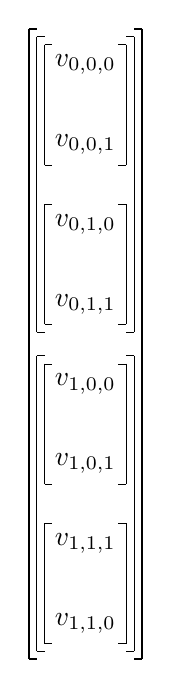
\begin{tikzpicture}[>=stealth,thick,baseline]
    \matrix [matrix of math nodes, row sep=1.5em, column sep=1.5em,](A){ 
    v_{0,0,0} \\
    v_{0,0,1} \\
    v_{0,1,0} \\
	v_{0,1,1} \\
	v_{1,0,0} \\
	v_{1,0,1} \\
	v_{1,1,1} \\ 
    v_{1,1,0} \\
    };
    

%	\draw (A-1-1.north west){}+(-0.1,+0.1) -- (A-1-1){}+(2,0);

	\draw[]  ($(A-1-1.north west) + (-0.2,+0.2)$) -- ($(A-8-1.south west) + (-0.2,-0.2)$);
	\draw[]  ($(A-1-1.north west) + (-0.2,+0.2)$) -- ++(0.1,0);
	\draw[]  ($(A-8-1.south west) + (-0.2,-0.2)$) -- ++(0.1,0); 	

	\draw[]  ($(A-1-1.north east) + (+0.2,+0.2)$) -- ($(A-8-1.south east) + (+0.2,-0.2)$);
	\draw[]  ($(A-1-1.north east) + (+0.2,+0.2)$) -- ++(-0.1,0);
	\draw[]  ($(A-8-1.south east) + (+0.2,-0.2)$) -- ++(-0.1,0); 	


	\draw[thin]  ($(A-1-1.north west) + (-0.1,+0.1)$) -- ($(A-4-1.south west) + (-0.1,-0.1)$);
	\draw[thin]  ($(A-1-1.north west) + (-0.1,+0.1)$) -- ++(0.1,0);
	\draw[thin]  ($(A-4-1.south west) + (-0.1,-0.1)$) -- ++(0.1,0);

	\draw[thin]  ($(A-5-1.north west) + (-0.1,+0.1)$) -- ($(A-8-1.south west) + (-0.1,-0.1)$);
	\draw[thin]  ($(A-5-1.north west) + (-0.1,+0.1)$) -- ++(0.1,0);
	\draw[thin]  ($(A-8-1.south west) + (-0.1,-0.1)$) -- ++(0.1,0);


	\draw[thin]  ($(A-1-1.north east) + (+0.1,+0.1)$) -- ($(A-4-1.south east) + (+0.1,-0.1)$);
	\draw[thin]  ($(A-1-1.north east) + (+0.1,+0.1)$) -- ++(-0.1,0);
	\draw[thin]  ($(A-4-1.south east) + (+0.1,-0.1)$) -- ++(-0.1,0);

	\draw[thin]  ($(A-5-1.north east) + (+0.1,+0.1)$) -- ($(A-8-1.south east) + (+0.1,-0.1)$);
	\draw[thin]  ($(A-5-1.north east) + (+0.1,+0.1)$) -- ++(-0.1,0);
	\draw[thin]  ($(A-8-1.south east) + (+0.1,-0.1)$) -- ++(-0.1,0);




	\draw[ultra thin]  (A-1-1.north west) -- ++(0.1,0);
	\draw[ultra thin]  (A-1-1.north west) -- 
	                   (A-2-1.south west);
	\draw[ultra thin]  (A-2-1.south west) -- ++(0.1,0);	
	
	\draw[ultra thin]  (A-1-1.north east) -- ++(-0.1,0);
	\draw[ultra thin]  (A-1-1.north east) -- 
	                   (A-2-1.south east);
	\draw[ultra thin]  (A-2-1.south east) -- ++(-0.1,0);	
	
	\draw[ultra thin]  (A-3-1.north west) -- ++(0.1,0);
	\draw[ultra thin]  (A-3-1.north west) -- 
	                   (A-4-1.south west);
	\draw[ultra thin]  (A-4-1.south west) -- ++(0.1,0);	
	
	\draw[ultra thin]  (A-3-1.north east) -- ++(-0.1,0);
	\draw[ultra thin]  (A-3-1.north east) -- 
	                   (A-4-1.south east);
	\draw[ultra thin]  (A-4-1.south east) -- ++(-0.1,0);	
	
	\draw[ultra thin]  (A-5-1.north west) -- ++(0.1,0);
	\draw[ultra thin]  (A-5-1.north west) -- 
	                   (A-6-1.south west);
	\draw[ultra thin]  (A-6-1.south west) -- ++(0.1,0);	
	
	\draw[ultra thin]  (A-5-1.north east) -- ++(-0.1,0);
	\draw[ultra thin]  (A-5-1.north east) -- 
	                   (A-6-1.south east);
	\draw[ultra thin]  (A-6-1.south east) -- ++(-0.1,0);	
	
	\draw[ultra thin]  (A-7-1.north west) -- ++(0.1,0);
	\draw[ultra thin]  (A-7-1.north west) -- 
	                   (A-8-1.south west);
	\draw[ultra thin]  (A-8-1.south west) -- ++(0.1,0);	
	
	\draw[ultra thin]  (A-7-1.north east) -- ++(-0.1,0);
	\draw[ultra thin]  (A-7-1.north east) -- 
	                   (A-8-1.south east);
	\draw[ultra thin]  (A-8-1.south east) -- ++(-0.1,0);	


    \end{tikzpicture}

    
    
\end{document}
    
    
    }} 
%=
%\text{\adjustbox{scale=0.75}{ \documentclass[border=5pt]{standalone}
     \usepackage[svgnames]{xcolor}
   
    \usepackage{tikz}
    \usetikzlibrary{matrix,decorations.pathreplacing, calc, positioning,fit}
    \usepackage{amsmath}
    \usepackage{mathtools}
 
    \begin{document}

    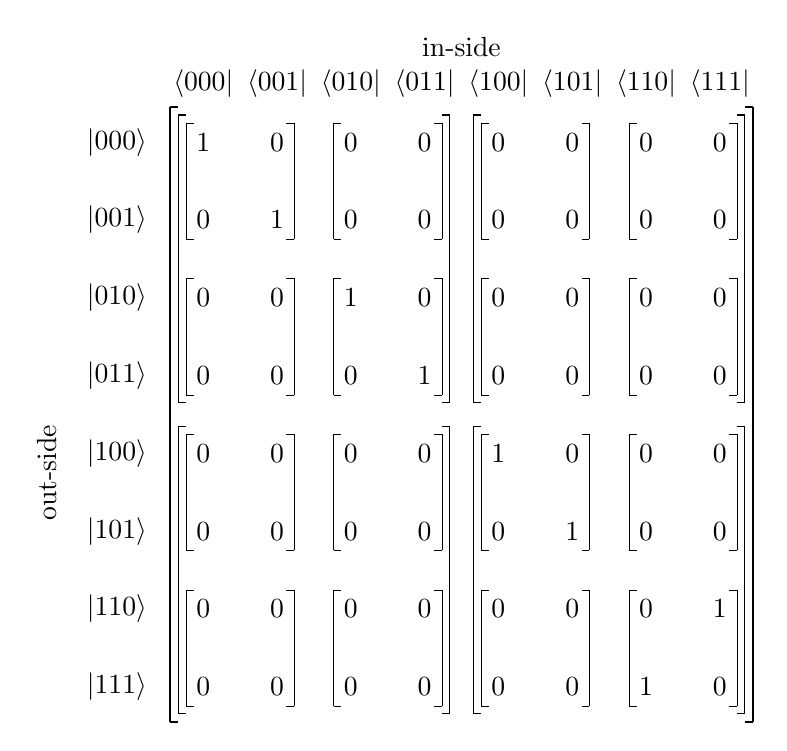
\begin{tikzpicture}[>=stealth,thick,baseline]
    \matrix [matrix of math nodes, row sep=1.5em, column sep=1.5em,](A){ 
    1&0&0&0&0&0&0&0 \\
    0&1&0&0&0&0&0&0 \\
    0&0&1&0&0&0&0&0 \\
	0&0&0&1&0&0&0&0 \\
	0&0&0&0&1&0&0&0 \\
	0&0&0&0&0&1&0&0 \\
	0&0&0&0&0&0&0&1 \\
    0&0&0&0&0&0&1&0 \\
    };

	\draw[]  ($(A-1-1.north west) + (-0.2,+0.2)$) -- ($(A-8-1.south west) + (-0.2,-0.2)$);
	\draw[]  ($(A-1-1.north west) + (-0.2,+0.2)$) -- ++(0.1,0);
	\draw[]  ($(A-8-1.south west) + (-0.2,-0.2)$) -- ++(0.1,0); 	

	\draw[]  ($(A-1-8.north east) + (+0.2,+0.2)$) -- ($(A-8-8.south east) + (+0.2,-0.2)$);
	\draw[]  ($(A-1-8.north east) + (+0.2,+0.2)$) -- ++(-0.1,0);
	\draw[]  ($(A-8-8.south east) + (+0.2,-0.2)$) -- ++(-0.1,0); 	


	\draw[thin]  ($(A-1-1.north west) + (-0.1,+0.1)$) -- ($(A-4-1.south west) + (-0.1,-0.1)$);
	\draw[thin]  ($(A-1-1.north west) + (-0.1,+0.1)$) -- ++(0.1,0);
	\draw[thin]  ($(A-4-1.south west) + (-0.1,-0.1)$) -- ++(0.1,0);

	\draw[thin]  ($(A-5-1.north west) + (-0.1,+0.1)$) -- ($(A-8-1.south west) + (-0.1,-0.1)$);
	\draw[thin]  ($(A-5-1.north west) + (-0.1,+0.1)$) -- ++(0.1,0);
	\draw[thin]  ($(A-8-1.south west) + (-0.1,-0.1)$) -- ++(0.1,0);

	\draw[thin]  ($(A-1-5.north west) + (-0.1,+0.1)$) -- ($(A-4-5.south west) + (-0.1,-0.1)$);
	\draw[thin]  ($(A-1-5.north west) + (-0.1,+0.1)$) -- ++(0.1,0);
	\draw[thin]  ($(A-4-5.south west) + (-0.1,-0.1)$) -- ++(0.1,0);

	\draw[thin]  ($(A-5-5.north west) + (-0.1,+0.1)$) -- ($(A-8-5.south west) + (-0.1,-0.1)$);
	\draw[thin]  ($(A-5-5.north west) + (-0.1,+0.1)$) -- ++(0.1,0);
	\draw[thin]  ($(A-8-5.south west) + (-0.1,-0.1)$) -- ++(0.1,0);


	\draw[thin]  ($(A-1-4.north east) + (+0.1,+0.1)$) -- ($(A-4-4.south east) + (+0.1,-0.1)$);
	\draw[thin]  ($(A-1-4.north east) + (+0.1,+0.1)$) -- ++(-0.1,0);
	\draw[thin]  ($(A-4-4.south east) + (+0.1,-0.1)$) -- ++(-0.1,0);

	\draw[thin]  ($(A-5-4.north east) + (+0.1,+0.1)$) -- ($(A-8-4.south east) + (+0.1,-0.1)$);
	\draw[thin]  ($(A-5-4.north east) + (+0.1,+0.1)$) -- ++(-0.1,0);
	\draw[thin]  ($(A-8-4.south east) + (+0.1,-0.1)$) -- ++(-0.1,0);


	\draw[thin]  ($(A-1-8.north east) + (+0.1,+0.1)$) -- ($(A-4-8.south east) + (+0.1,-0.1)$);
	\draw[thin]  ($(A-1-8.north east) + (+0.1,+0.1)$) -- ++(-0.1,0);
	\draw[thin]  ($(A-4-8.south east) + (+0.1,-0.1)$) -- ++(-0.1,0);

	\draw[thin]  ($(A-5-8.north east) + (+0.1,+0.1)$) -- ($(A-8-8.south east) + (+0.1,-0.1)$);
	\draw[thin]  ($(A-5-8.north east) + (+0.1,+0.1)$) -- ++(-0.1,0);
	\draw[thin]  ($(A-8-8.south east) + (+0.1,-0.1)$) -- ++(-0.1,0);


	\draw[ultra thin]  (A-1-1.north west) -- ++(0.1,0);
	\draw[ultra thin]  (A-1-1.north west) -- 
	                   (A-2-1.south west);
	\draw[ultra thin]  (A-2-1.south west) -- ++(0.1,0);	
	
	\draw[ultra thin]  (A-1-2.north east) -- ++(-0.1,0);
	\draw[ultra thin]  (A-1-2.north east) -- 
	                   (A-2-2.south east);
	\draw[ultra thin]  (A-2-2.south east) -- ++(-0.1,0);	
	
	\draw[ultra thin]  (A-3-1.north west) -- ++(0.1,0);
	\draw[ultra thin]  (A-3-1.north west) -- 
	                   (A-4-1.south west);
	\draw[ultra thin]  (A-4-1.south west) -- ++(0.1,0);	
	
	\draw[ultra thin]  (A-3-2.north east) -- ++(-0.1,0);
	\draw[ultra thin]  (A-3-2.north east) -- 
	                   (A-4-2.south east);
	\draw[ultra thin]  (A-4-2.south east) -- ++(-0.1,0);	
	
	\draw[ultra thin]  (A-5-1.north west) -- ++(0.1,0);
	\draw[ultra thin]  (A-5-1.north west) -- 
	                   (A-6-1.south west);
	\draw[ultra thin]  (A-6-1.south west) -- ++(0.1,0);	
	
	\draw[ultra thin]  (A-5-2.north east) -- ++(-0.1,0);
	\draw[ultra thin]  (A-5-2.north east) -- 
	                   (A-6-2.south east);
	\draw[ultra thin]  (A-6-2.south east) -- ++(-0.1,0);	
	
	\draw[ultra thin]  (A-7-1.north west) -- ++(0.1,0);
	\draw[ultra thin]  (A-7-1.north west) -- 
	                   (A-8-1.south west);
	\draw[ultra thin]  (A-8-1.south west) -- ++(0.1,0);	
	
	\draw[ultra thin]  (A-7-2.north east) -- ++(-0.1,0);
	\draw[ultra thin]  (A-7-2.north east) -- 
	                   (A-8-2.south east);
	\draw[ultra thin]  (A-8-2.south east) -- ++(-0.1,0);	


	\draw[ultra thin]  (A-1-3.north west) -- ++(0.1,0);
	\draw[ultra thin]  (A-1-3.north west) -- 
	                   (A-2-3.south west);
	\draw[ultra thin]  (A-2-3.south west) -- ++(0.1,0);	
	
	\draw[ultra thin]  (A-1-4.north east) -- ++(-0.1,0);
	\draw[ultra thin]  (A-1-4.north east) -- 
	                   (A-2-4.south east);
	\draw[ultra thin]  (A-2-4.south east) -- ++(-0.1,0);	
	
	\draw[ultra thin]  (A-3-3.north west) -- ++(0.1,0);
	\draw[ultra thin]  (A-3-3.north west) -- 
	                   (A-4-3.south west);
	\draw[ultra thin]  (A-4-3.south west) -- ++(0.1,0);	
	
	\draw[ultra thin]  (A-3-4.north east) -- ++(-0.1,0);
	\draw[ultra thin]  (A-3-4.north east) -- 
	                   (A-4-4.south east);
	\draw[ultra thin]  (A-4-4.south east) -- ++(-0.1,0);	
	
	\draw[ultra thin]  (A-5-3.north west) -- ++(0.1,0);
	\draw[ultra thin]  (A-5-3.north west) -- 
	                   (A-6-3.south west);
	\draw[ultra thin]  (A-6-3.south west) -- ++(0.1,0);	
	
	\draw[ultra thin]  (A-5-4.north east) -- ++(-0.1,0);
	\draw[ultra thin]  (A-5-4.north east) -- 
	                   (A-6-4.south east);
	\draw[ultra thin]  (A-6-4.south east) -- ++(-0.1,0);	
	
	\draw[ultra thin]  (A-7-3.north west) -- ++(0.1,0);
	\draw[ultra thin]  (A-7-3.north west) -- 
	                   (A-8-3.south west);
	\draw[ultra thin]  (A-8-3.south west) -- ++(0.1,0);	
	
	\draw[ultra thin]  (A-7-4.north east) -- ++(-0.1,0);
	\draw[ultra thin]  (A-7-4.north east) -- 
	                   (A-8-4.south east);
	\draw[ultra thin]  (A-8-4.south east) -- ++(-0.1,0);	
	

	\draw[ultra thin]  (A-1-3.north west) -- ++(0.1,0);
	\draw[ultra thin]  (A-1-3.north west) -- 
	                   (A-2-3.south west);
	\draw[ultra thin]  (A-2-3.south west) -- ++(0.1,0);	
	
	\draw[ultra thin]  (A-1-4.north east) -- ++(-0.1,0);
	\draw[ultra thin]  (A-1-4.north east) -- 
	                   (A-2-4.south east);
	\draw[ultra thin]  (A-2-4.south east) -- ++(-0.1,0);	
	
	\draw[ultra thin]  (A-3-3.north west) -- ++(0.1,0);
	\draw[ultra thin]  (A-3-3.north west) -- 
	                   (A-4-3.south west);
	\draw[ultra thin]  (A-4-3.south west) -- ++(0.1,0);	
	
	\draw[ultra thin]  (A-3-4.north east) -- ++(-0.1,0);
	\draw[ultra thin]  (A-3-4.north east) -- 
	                   (A-4-4.south east);
	\draw[ultra thin]  (A-4-4.south east) -- ++(-0.1,0);	
	
	\draw[ultra thin]  (A-5-3.north west) -- ++(0.1,0);
	\draw[ultra thin]  (A-5-3.north west) -- 
	                   (A-6-3.south west);
	\draw[ultra thin]  (A-6-3.south west) -- ++(0.1,0);	
	
	\draw[ultra thin]  (A-5-4.north east) -- ++(-0.1,0);
	\draw[ultra thin]  (A-5-4.north east) -- 
	                   (A-6-4.south east);
	\draw[ultra thin]  (A-6-4.south east) -- ++(-0.1,0);	
	
	\draw[ultra thin]  (A-7-3.north west) -- ++(0.1,0);
	\draw[ultra thin]  (A-7-3.north west) -- 
	                   (A-8-3.south west);
	\draw[ultra thin]  (A-8-3.south west) -- ++(0.1,0);	
	
	\draw[ultra thin]  (A-7-4.north east) -- ++(-0.1,0);
	\draw[ultra thin]  (A-7-4.north east) -- 
	                   (A-8-4.south east);
	\draw[ultra thin]  (A-8-4.south east) -- ++(-0.1,0);	
	
	

	\draw[ultra thin]  (A-1-5.north west) -- ++(0.1,0);
	\draw[ultra thin]  (A-1-5.north west) -- 
	                   (A-2-5.south west);
	\draw[ultra thin]  (A-2-5.south west) -- ++(0.1,0);	
	
	\draw[ultra thin]  (A-1-6.north east) -- ++(-0.1,0);
	\draw[ultra thin]  (A-1-6.north east) -- 
	                   (A-2-6.south east);
	\draw[ultra thin]  (A-2-6.south east) -- ++(-0.1,0);	
	
	\draw[ultra thin]  (A-3-5.north west) -- ++(0.1,0);
	\draw[ultra thin]  (A-3-5.north west) -- 
	                   (A-4-5.south west);
	\draw[ultra thin]  (A-4-5.south west) -- ++(0.1,0);	
	
	\draw[ultra thin]  (A-3-6.north east) -- ++(-0.1,0);
	\draw[ultra thin]  (A-3-6.north east) -- 
	                   (A-4-6.south east);
	\draw[ultra thin]  (A-4-6.south east) -- ++(-0.1,0);	
	
	\draw[ultra thin]  (A-5-5.north west) -- ++(0.1,0);
	\draw[ultra thin]  (A-5-5.north west) -- 
	                   (A-6-5.south west);
	\draw[ultra thin]  (A-6-5.south west) -- ++(0.1,0);	
	
	\draw[ultra thin]  (A-5-6.north east) -- ++(-0.1,0);
	\draw[ultra thin]  (A-5-6.north east) -- 
	                   (A-6-6.south east);
	\draw[ultra thin]  (A-6-6.south east) -- ++(-0.1,0);	
	
	\draw[ultra thin]  (A-7-5.north west) -- ++(0.1,0);
	\draw[ultra thin]  (A-7-5.north west) -- 
	                   (A-8-5.south west);
	\draw[ultra thin]  (A-8-5.south west) -- ++(0.1,0);	
	
	\draw[ultra thin]  (A-7-6.north east) -- ++(-0.1,0);
	\draw[ultra thin]  (A-7-6.north east) -- 
	                   (A-8-6.south east);
	\draw[ultra thin]  (A-8-6.south east) -- ++(-0.1,0);	
		
	
	
	
	
	\draw[ultra thin]  (A-1-7.north west) -- ++(0.1,0);
	\draw[ultra thin]  (A-1-7.north west) -- 
	                   (A-2-7.south west);
	\draw[ultra thin]  (A-2-7.south west) -- ++(0.1,0);	
	
	\draw[ultra thin]  (A-1-8.north east) -- ++(-0.1,0);
	\draw[ultra thin]  (A-1-8.north east) -- 
	                   (A-2-8.south east);
	\draw[ultra thin]  (A-2-8.south east) -- ++(-0.1,0);	
	
	\draw[ultra thin]  (A-3-7.north west) -- ++(0.1,0);
	\draw[ultra thin]  (A-3-7.north west) -- 
	                   (A-4-7.south west);
	\draw[ultra thin]  (A-4-7.south west) -- ++(0.1,0);	
	
	\draw[ultra thin]  (A-3-8.north east) -- ++(-0.1,0);
	\draw[ultra thin]  (A-3-8.north east) -- 
	                   (A-4-8.south east);
	\draw[ultra thin]  (A-4-8.south east) -- ++(-0.1,0);	
	
	\draw[ultra thin]  (A-5-7.north west) -- ++(0.1,0);
	\draw[ultra thin]  (A-5-7.north west) -- 
	                   (A-6-7.south west);
	\draw[ultra thin]  (A-6-7.south west) -- ++(0.1,0);	
	
	\draw[ultra thin]  (A-5-8.north east) -- ++(-0.1,0);
	\draw[ultra thin]  (A-5-8.north east) -- 
	                   (A-6-8.south east);
	\draw[ultra thin]  (A-6-8.south east) -- ++(-0.1,0);	
	
	\draw[ultra thin]  (A-7-7.north west) -- ++(0.1,0);
	\draw[ultra thin]  (A-7-7.north west) -- 
	                   (A-8-7.south west);
	\draw[ultra thin]  (A-8-7.south west) -- ++(0.1,0);	
	
	\draw[ultra thin]  (A-7-8.north east) -- ++(-0.1,0);
	\draw[ultra thin]  (A-7-8.north east) -- 
	                   (A-8-8.south east);
	\draw[ultra thin]  (A-8-8.south east) -- ++(-0.1,0);	
	
	
   \node[
     fit=(A-1-4)(A-1-5),
     inner xsep=5pt,inner ysep=20pt,
     label=above: in-side   
     ](K01) {};

   \node[
     fit=(A-4-1)(A-5-1),
     inner xsep=50pt,inner ysep=-5pt,
     label={[rotate=90]left:out-side}
     ](K01) {};




   \node[
     fit=(A-1-1)(A-1-1),
     inner xsep=5pt,inner ysep=5pt,
     label=above: $\langle 000|$
    ](K00) {};

   \node[
     fit=(A-1-2)(A-1-2),
     inner xsep=5pt,inner ysep=5pt,
     label=above: $\langle 001|$
    ](K01) {};


   \node[
     fit=(A-1-3)(A-1-3),
     inner xsep=5pt,inner ysep=5pt,
     label=above: $\langle 010|$
    ](K10) {};

   \node[
     fit=(A-1-4)(A-1-4),
     inner xsep=5pt,inner ysep=5pt,
     label=above: $\langle 011|$
    ](K10) {};


   \node[
     fit=(A-1-5)(A-1-5),
     inner xsep=5pt,inner ysep=5pt,
     label=above: $\langle 100|$
    ](K00) {};

   \node[
     fit=(A-1-6)(A-1-6),
     inner xsep=5pt,inner ysep=5pt,
     label=above: $\langle 101|$
    ](K01) {};

   \node[
     fit=(A-1-7)(A-1-7),
     inner xsep=5pt,inner ysep=5pt,
     label=above: $\langle 110|$
    ](K10) {};
   \node[
     fit=(A-1-8)(A-1-8),
     inner xsep=5pt,inner ysep=5pt,
     label=above: $\langle 111|$
    ](K11) {};


   \node[
     fit=(A-1-1)(A-1-1),
     inner xsep=10pt,inner ysep=5pt,
     label=left: $|000\rangle$
    ](K00) {};

   \node[
     fit=(A-2-1)(A-2-1),
     inner xsep=10pt,inner ysep=5pt,
     label=left: $|001\rangle$
    ](K01) {};


   \node[
     fit=(A-3-1)(A-3-1),
     inner xsep=10pt,inner ysep=5pt,
     label=left: $|010\rangle$
    ](K10) {};


   \node[
     fit=(A-4-1)(A-4-1),
     inner xsep=10pt,inner ysep=5pt,
     label=left: $|011\rangle$
    ](K11) {};


   \node[
     fit=(A-5-1)(A-5-1),
     inner xsep=10pt,inner ysep=5pt,
     label=left: $|100\rangle$
    ](K00) {};

   \node[
     fit=(A-6-1)(A-6-1),
     inner xsep=10pt,inner ysep=5pt,
     label=left: $|101\rangle$
    ](K01) {};


   \node[
     fit=(A-7-1)(A-7-1),
     inner xsep=10pt,inner ysep=5pt,
     label=left: $|110\rangle$
    ](K10) {};


   \node[
     fit=(A-8-1)(A-8-1),
     inner xsep=10pt,inner ysep=5pt,
     label=left: $|111\rangle$
    ](K11) {};


    \end{tikzpicture}

\end{document}
    
    
    }}
%\bullet
%\text{\adjustbox{scale=0.75}{ \documentclass[border=5pt]{standalone}
     \usepackage[svgnames]{xcolor}
   
    \usepackage{tikz}
    \usetikzlibrary{matrix,decorations.pathreplacing, calc, positioning,fit}
    \usepackage{amsmath}
    \usepackage{mathtools}
 
    \begin{document}

    
   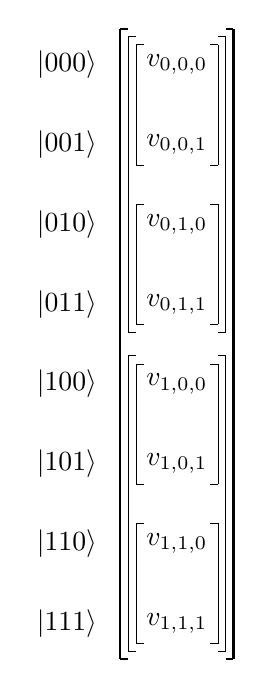
\begin{tikzpicture}[>=stealth,thick,baseline]
    \matrix [matrix of math nodes, row sep=1.5em, column sep=1.5em,](A){ 
    v_{0,0,0} \\
    v_{0,0,1} \\
    v_{0,1,0} \\
	v_{0,1,1} \\
	v_{1,0,0} \\
	v_{1,0,1} \\
	v_{1,1,0} \\ 
    v_{1,1,1} \\
    };
    

%	\draw (A-1-1.north west){}+(-0.1,+0.1) -- (A-1-1){}+(2,0);

	\draw[]  ($(A-1-1.north west) + (-0.2,+0.2)$) -- ($(A-8-1.south west) + (-0.2,-0.2)$);
	\draw[]  ($(A-1-1.north west) + (-0.2,+0.2)$) -- ++(0.1,0);
	\draw[]  ($(A-8-1.south west) + (-0.2,-0.2)$) -- ++(0.1,0); 	

	\draw[]  ($(A-1-1.north east) + (+0.2,+0.2)$) -- ($(A-8-1.south east) + (+0.2,-0.2)$);
	\draw[]  ($(A-1-1.north east) + (+0.2,+0.2)$) -- ++(-0.1,0);
	\draw[]  ($(A-8-1.south east) + (+0.2,-0.2)$) -- ++(-0.1,0); 	


	\draw[thin]  ($(A-1-1.north west) + (-0.1,+0.1)$) -- ($(A-4-1.south west) + (-0.1,-0.1)$);
	\draw[thin]  ($(A-1-1.north west) + (-0.1,+0.1)$) -- ++(0.1,0);
	\draw[thin]  ($(A-4-1.south west) + (-0.1,-0.1)$) -- ++(0.1,0);

	\draw[thin]  ($(A-5-1.north west) + (-0.1,+0.1)$) -- ($(A-8-1.south west) + (-0.1,-0.1)$);
	\draw[thin]  ($(A-5-1.north west) + (-0.1,+0.1)$) -- ++(0.1,0);
	\draw[thin]  ($(A-8-1.south west) + (-0.1,-0.1)$) -- ++(0.1,0);


	\draw[thin]  ($(A-1-1.north east) + (+0.1,+0.1)$) -- ($(A-4-1.south east) + (+0.1,-0.1)$);
	\draw[thin]  ($(A-1-1.north east) + (+0.1,+0.1)$) -- ++(-0.1,0);
	\draw[thin]  ($(A-4-1.south east) + (+0.1,-0.1)$) -- ++(-0.1,0);

	\draw[thin]  ($(A-5-1.north east) + (+0.1,+0.1)$) -- ($(A-8-1.south east) + (+0.1,-0.1)$);
	\draw[thin]  ($(A-5-1.north east) + (+0.1,+0.1)$) -- ++(-0.1,0);
	\draw[thin]  ($(A-8-1.south east) + (+0.1,-0.1)$) -- ++(-0.1,0);




	\draw[ultra thin]  (A-1-1.north west) -- ++(0.1,0);
	\draw[ultra thin]  (A-1-1.north west) -- 
	                   (A-2-1.south west);
	\draw[ultra thin]  (A-2-1.south west) -- ++(0.1,0);	
	
	\draw[ultra thin]  (A-1-1.north east) -- ++(-0.1,0);
	\draw[ultra thin]  (A-1-1.north east) -- 
	                   (A-2-1.south east);
	\draw[ultra thin]  (A-2-1.south east) -- ++(-0.1,0);	
	
	\draw[ultra thin]  (A-3-1.north west) -- ++(0.1,0);
	\draw[ultra thin]  (A-3-1.north west) -- 
	                   (A-4-1.south west);
	\draw[ultra thin]  (A-4-1.south west) -- ++(0.1,0);	
	
	\draw[ultra thin]  (A-3-1.north east) -- ++(-0.1,0);
	\draw[ultra thin]  (A-3-1.north east) -- 
	                   (A-4-1.south east);
	\draw[ultra thin]  (A-4-1.south east) -- ++(-0.1,0);	
	
	\draw[ultra thin]  (A-5-1.north west) -- ++(0.1,0);
	\draw[ultra thin]  (A-5-1.north west) -- 
	                   (A-6-1.south west);
	\draw[ultra thin]  (A-6-1.south west) -- ++(0.1,0);	
	
	\draw[ultra thin]  (A-5-1.north east) -- ++(-0.1,0);
	\draw[ultra thin]  (A-5-1.north east) -- 
	                   (A-6-1.south east);
	\draw[ultra thin]  (A-6-1.south east) -- ++(-0.1,0);	
	
	\draw[ultra thin]  (A-7-1.north west) -- ++(0.1,0);
	\draw[ultra thin]  (A-7-1.north west) -- 
	                   (A-8-1.south west);
	\draw[ultra thin]  (A-8-1.south west) -- ++(0.1,0);	
	
	\draw[ultra thin]  (A-7-1.north east) -- ++(-0.1,0);
	\draw[ultra thin]  (A-7-1.north east) -- 
	                   (A-8-1.south east);
	\draw[ultra thin]  (A-8-1.south east) -- ++(-0.1,0);	


   \node[
     fit=(A-1-1)(A-1-1),
     inner xsep=10pt,inner ysep=5pt,
     label=left: $|000\rangle$
    ](K00) {};

   \node[
     fit=(A-2-1)(A-2-1),
     inner xsep=10pt,inner ysep=5pt,
     label=left: $|001\rangle$
    ](K01) {};


   \node[
     fit=(A-3-1)(A-3-1),
     inner xsep=10pt,inner ysep=5pt,
     label=left: $|010\rangle$
    ](K10) {};


   \node[
     fit=(A-4-1)(A-4-1),
     inner xsep=10pt,inner ysep=5pt,
     label=left: $|011\rangle$
    ](K11) {};


   \node[
     fit=(A-5-1)(A-5-1),
     inner xsep=10pt,inner ysep=5pt,
     label=left: $|100\rangle$
    ](K00) {};

   \node[
     fit=(A-6-1)(A-6-1),
     inner xsep=10pt,inner ysep=5pt,
     label=left: $|101\rangle$
    ](K01) {};


   \node[
     fit=(A-7-1)(A-7-1),
     inner xsep=10pt,inner ysep=5pt,
     label=left: $|110\rangle$
    ](K10) {};


   \node[
     fit=(A-8-1)(A-8-1),
     inner xsep=10pt,inner ysep=5pt,
     label=left: $|111\rangle$
    ](K11) {};

%   \node[
%     fit=(A-6-4)(A-6-4),
%     inner xsep=20pt,inner ysep=20pt,
%     label=below: $j$-ième colonne
%     ](C) {};
%
%    \draw[->](L.east)-- (A-4-4);
%    \draw[->](C.south)-- (A-4-4);

    \end{tikzpicture}

    
    
\end{document}
    
    
    }}
%\]
%%=  \dot  \documentclass[border=5pt]{standalone}
     \usepackage[svgnames]{xcolor}
   
    \usepackage{tikz}
    \usetikzlibrary{matrix,decorations.pathreplacing, calc, positioning,fit}
    \usepackage{amsmath}
    \usepackage{mathtools}
 
    \begin{document}

    
   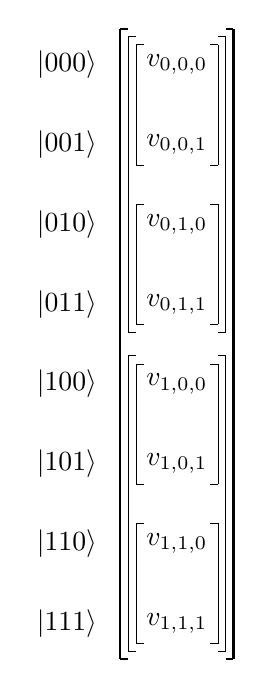
\begin{tikzpicture}[>=stealth,thick,baseline]
    \matrix [matrix of math nodes, row sep=1.5em, column sep=1.5em,](A){ 
    v_{0,0,0} \\
    v_{0,0,1} \\
    v_{0,1,0} \\
	v_{0,1,1} \\
	v_{1,0,0} \\
	v_{1,0,1} \\
	v_{1,1,0} \\ 
    v_{1,1,1} \\
    };
    

%	\draw (A-1-1.north west){}+(-0.1,+0.1) -- (A-1-1){}+(2,0);

	\draw[]  ($(A-1-1.north west) + (-0.2,+0.2)$) -- ($(A-8-1.south west) + (-0.2,-0.2)$);
	\draw[]  ($(A-1-1.north west) + (-0.2,+0.2)$) -- ++(0.1,0);
	\draw[]  ($(A-8-1.south west) + (-0.2,-0.2)$) -- ++(0.1,0); 	

	\draw[]  ($(A-1-1.north east) + (+0.2,+0.2)$) -- ($(A-8-1.south east) + (+0.2,-0.2)$);
	\draw[]  ($(A-1-1.north east) + (+0.2,+0.2)$) -- ++(-0.1,0);
	\draw[]  ($(A-8-1.south east) + (+0.2,-0.2)$) -- ++(-0.1,0); 	


	\draw[thin]  ($(A-1-1.north west) + (-0.1,+0.1)$) -- ($(A-4-1.south west) + (-0.1,-0.1)$);
	\draw[thin]  ($(A-1-1.north west) + (-0.1,+0.1)$) -- ++(0.1,0);
	\draw[thin]  ($(A-4-1.south west) + (-0.1,-0.1)$) -- ++(0.1,0);

	\draw[thin]  ($(A-5-1.north west) + (-0.1,+0.1)$) -- ($(A-8-1.south west) + (-0.1,-0.1)$);
	\draw[thin]  ($(A-5-1.north west) + (-0.1,+0.1)$) -- ++(0.1,0);
	\draw[thin]  ($(A-8-1.south west) + (-0.1,-0.1)$) -- ++(0.1,0);


	\draw[thin]  ($(A-1-1.north east) + (+0.1,+0.1)$) -- ($(A-4-1.south east) + (+0.1,-0.1)$);
	\draw[thin]  ($(A-1-1.north east) + (+0.1,+0.1)$) -- ++(-0.1,0);
	\draw[thin]  ($(A-4-1.south east) + (+0.1,-0.1)$) -- ++(-0.1,0);

	\draw[thin]  ($(A-5-1.north east) + (+0.1,+0.1)$) -- ($(A-8-1.south east) + (+0.1,-0.1)$);
	\draw[thin]  ($(A-5-1.north east) + (+0.1,+0.1)$) -- ++(-0.1,0);
	\draw[thin]  ($(A-8-1.south east) + (+0.1,-0.1)$) -- ++(-0.1,0);




	\draw[ultra thin]  (A-1-1.north west) -- ++(0.1,0);
	\draw[ultra thin]  (A-1-1.north west) -- 
	                   (A-2-1.south west);
	\draw[ultra thin]  (A-2-1.south west) -- ++(0.1,0);	
	
	\draw[ultra thin]  (A-1-1.north east) -- ++(-0.1,0);
	\draw[ultra thin]  (A-1-1.north east) -- 
	                   (A-2-1.south east);
	\draw[ultra thin]  (A-2-1.south east) -- ++(-0.1,0);	
	
	\draw[ultra thin]  (A-3-1.north west) -- ++(0.1,0);
	\draw[ultra thin]  (A-3-1.north west) -- 
	                   (A-4-1.south west);
	\draw[ultra thin]  (A-4-1.south west) -- ++(0.1,0);	
	
	\draw[ultra thin]  (A-3-1.north east) -- ++(-0.1,0);
	\draw[ultra thin]  (A-3-1.north east) -- 
	                   (A-4-1.south east);
	\draw[ultra thin]  (A-4-1.south east) -- ++(-0.1,0);	
	
	\draw[ultra thin]  (A-5-1.north west) -- ++(0.1,0);
	\draw[ultra thin]  (A-5-1.north west) -- 
	                   (A-6-1.south west);
	\draw[ultra thin]  (A-6-1.south west) -- ++(0.1,0);	
	
	\draw[ultra thin]  (A-5-1.north east) -- ++(-0.1,0);
	\draw[ultra thin]  (A-5-1.north east) -- 
	                   (A-6-1.south east);
	\draw[ultra thin]  (A-6-1.south east) -- ++(-0.1,0);	
	
	\draw[ultra thin]  (A-7-1.north west) -- ++(0.1,0);
	\draw[ultra thin]  (A-7-1.north west) -- 
	                   (A-8-1.south west);
	\draw[ultra thin]  (A-8-1.south west) -- ++(0.1,0);	
	
	\draw[ultra thin]  (A-7-1.north east) -- ++(-0.1,0);
	\draw[ultra thin]  (A-7-1.north east) -- 
	                   (A-8-1.south east);
	\draw[ultra thin]  (A-8-1.south east) -- ++(-0.1,0);	


   \node[
     fit=(A-1-1)(A-1-1),
     inner xsep=10pt,inner ysep=5pt,
     label=left: $|000\rangle$
    ](K00) {};

   \node[
     fit=(A-2-1)(A-2-1),
     inner xsep=10pt,inner ysep=5pt,
     label=left: $|001\rangle$
    ](K01) {};


   \node[
     fit=(A-3-1)(A-3-1),
     inner xsep=10pt,inner ysep=5pt,
     label=left: $|010\rangle$
    ](K10) {};


   \node[
     fit=(A-4-1)(A-4-1),
     inner xsep=10pt,inner ysep=5pt,
     label=left: $|011\rangle$
    ](K11) {};


   \node[
     fit=(A-5-1)(A-5-1),
     inner xsep=10pt,inner ysep=5pt,
     label=left: $|100\rangle$
    ](K00) {};

   \node[
     fit=(A-6-1)(A-6-1),
     inner xsep=10pt,inner ysep=5pt,
     label=left: $|101\rangle$
    ](K01) {};


   \node[
     fit=(A-7-1)(A-7-1),
     inner xsep=10pt,inner ysep=5pt,
     label=left: $|110\rangle$
    ](K10) {};


   \node[
     fit=(A-8-1)(A-8-1),
     inner xsep=10pt,inner ysep=5pt,
     label=left: $|111\rangle$
    ](K11) {};

%   \node[
%     fit=(A-6-4)(A-6-4),
%     inner xsep=20pt,inner ysep=20pt,
%     label=below: $j$-ième colonne
%     ](C) {};
%
%    \draw[->](L.east)-- (A-4-4);
%    \draw[->](C.south)-- (A-4-4);

    \end{tikzpicture}

    
    
\end{document}
    
    
    
%
%
%\[
%\ket{v'} = U\cdot \ket{v}
%\]
%
%\[
%v'_{a} = U_{a,b} \cdot v_{b}
%\]
%
%
%\[
%v'_{i,j,k} = U_{i,j,k;l,m,n} \cdot v_{l,m,n}
%\]

\subsection{Additional reading}
The canonical textbook for quantum computing and information remains Michael A. Nielsen's and Isaac L. Chuang's   
classic ``Quantum Computation and Quantum Information'' (affectionately know as Mike and Ike)~\cite{Nielsen2000a}.  
If you have any serious interest in quantum computing, you should own this book\endnote{And Mike and Ike.}.
% We're 
These notes are 
going to take a different cut through the subject, with more detail in some places, some newer material, but neglecting other areas, since it is not necessary to repeat what Mike and Ike have already so ably covered. John Preskill's lecture notes~\cite{PreskillLectureNotes} are another excellent (If perennially incomplete) treatment of the subject.

For a basic introduction to quantum mechanics, see ``Quantum Mechanics: The Theoretical Minimum''
by Leonard Susskind and Art Friedman~\cite{Susskind2015a}. The traditional quantum mechanics textbooks are not so useful, since they tend to rapidly skip over the fundamental and informational aspects, and concentrate on the detailed behavior of light, and atoms, and cavities, and what have you. Such physical details  are important if you're building a quantum computer, obviously, but not so much for programming one, and I think the traditional approach tends to obscure the essentials of quantum information and how fundamentally different quantum is from classical physics. But among such physics texts, I'd recommend ``Modern Quantum Mechanics'' by J.~J.~Sakurai~\cite{Sakurai2010a}.

For gentler introductions to quantum computing see ``Quantum Computing: A Gentle Introduction'' by Eleanor G. Rieffel and Wolfgang H. Polak~\cite{Rieffel2014a}. 
Another interesting take is ``Quantum Country'' by Andy Matuschak and Michael Nielsen. This is an online introductory course in quantum computing, with builtin spaced repetition~\cite{QuantumCountry}. Scott Aaronson's ``Quantum Computing since Democritus''~\cite{Aaronson2013a} is also a good place to start, particularly for computational complexity theory.

%     


Mathematically, quantum mechanics is mostly applied linear algebra, and you can never go wrong learning more linear algebra. For a good introduction see ``No Bullshit Guide to Linear Algebra'' by Ivan Savov~\cite{Savov2017a}, and for a deeper dive ``Linear Algebra Done Right'' by Sheldon Axler~\cite{Axler2015a}.


For a deep dives into quantum information, both ``The Theory of Quantum Information'' by John Watrous~\cite{Watrous2018a} and ``Quantum Information Theory'' by Mark M.~Wilde~\cite{Wilde2017a} are excellent, if weighty, tombs.

And if you have very young children, start them early with Chris Ferrie and whurely's ``Quantum Computing for Babies''~\cite{Ferrie2018a}.


%
% !TEX encoding = UTF-8 Unicode 
% !TEX root = on_gates.tex

\clearpage

\section{Mathematical structures of quantum mechanics}


\subsection{Groups}
 A \define{group} consists of two things
 \begin{enumerate}
\item A set of objects, $G$, whose elements we will label $x$, $y$, $z$, etc.
\item A composition rule (called the {\sl product}) that maps pairs of objects in $G$ to another element of $G$, $xy=z$
\end{enumerate}
which are subject to the following conditions:
\begin{enumerate}
\item The product is associative: $x(yz)= (xy)z= xyz$
\item $G$ contains an identity element $e$, so that $ex=xe=x$ for all elements $x$ in $G$.
\item All elements have an inverse, generally written $x^{-1}$, such that $x^{-1}x = x x^{-1} = e$.
\end{enumerate}

{\sl Example:} The positive and negative integers $..., -2, -1, 0, 1, 2, ...$ form a group under addition $+$, called the {\sl additive group of integers}. Here the identity element is zero $0+x=x$, and negation is inversion, $x+(-x) = 0$. When a group composition rule is commutative, $x+y = y+x$ we call the group {\sl abelian}.
The non-negative integers do not form a group under addition, since there are no inverses. The positive-integers under addition have neither inverses nor an identity element.


{\sl Example:} The real numbers also form a group under multiplication, with $1$ as the identity element, and reciprocals as inverse elements, $x^{-1} = \tfrac{1}{x}$.

{\sl Example:} Let $G$ be the collection of all permutations of $n$ objects, and the group product the composition of permutations. Then we have a {\sl permutation group} called $S_n$ with $n!$ elements.
 
The {\sl order} of a group is the number of elements in $G$, written $|G|$. A {\sl finite group} is a group with a finite number of elements. We'll encounter various examples presently, such as the octahedral, Pauli, Clifford and Weyl groups. An {\sl infinite group} has an infinite number of elements. The most important examples in quantum mechanics are the unitary groups of all unitary matrices of a given size.

% TODO: direct product, subgroups, quotient group



\subsection{Vector spaces}
A {\sl vector space} consists of three things:
  \begin{enumerate}
 \item A set $V$ whose elements are called {\sl vectors}.
 \item A composition rule for the summation of vectors to give another vector, written $u+v=w$.
 \item A composition rule (called  scalar multiplication) that maps a vector $v$ and a number $c$ to another vector written $cv$.
 \end{enumerate}
subject to the following conditions:
  \begin{enumerate}
  \item The set $V$ is an abelian group under addition. (The inverse of $v$ is written $-v$, and the identity element is written $0$.)
  \item The addition of numbers is distributive over multiplication by vectors, $(a+c)v=av + cv$.
  \item The summation of vectors is distributive over multiplication by numbers, $c(u+v)=cu + cv$.
  \item Scalar multiplication is associative, $a (cv) = (ac) v$. 
 \item The number $1$ is the identity for scaler multiplication, $1v=v$.
 \end{enumerate}
 For obscure historical reasons, in the context of vector spaces numbers are called \define{scalars}.
These numbers can be either real, in which case we have a \define{real vector space}, or complex, which gives a \define{complex vector space}. Scalars can also be some other number like structures, but such constructions don't seem to turn up much in practice.

{\sl Example:} Lists of numbers, $v=(v_1, v_2, ..., v_n)$ form a vector space with vector summation as element wise addition $u+v = (u_1+v_1, u_2 +v_2, ..., u_n+ v_n)$, and scalar multiplication distributed over elements, $c(v_1, v_2, ..., v_n) =(cv_1, cv_2, ..., cv_n)$. This is the most common computational representation of vectors, but we should not confuse such concrete realizations with the Platonic ideal of the mathematical structure.

The {\sl dimension} of a vector space is the minimum number of {\sl basis vectors} from which the entire set of vectors can be constructed using vector summation and scalar multiplication. For lists of $n$ arbitrary numbers, the dimension of the vector space is $n$, but we could be could be restricted to some \define{subspace} which has a lower dimension.



\subsection{Hilbert spaces}

A {\sl Hilbert space} consists of two things:

 \begin{enumerate}
 \item A complex vector space $H$.
 \item A composition rule that maps pairs of vectors in $H$ to a complex number, called the \define{inner product}, and written $(g,h)=c$.
 \end{enumerate}
 subject to the following conditions:
 \begin{enumerate}
 \item Complex conjugation of the inner product transposes the arguments, $(g, h)^* = (h, g)$. (Thus the number $c=(h,h)=(h,h)^*$ must be real.)
 \item For any non-zero vector $h$, the inner product $(h,h)$ must be positive. 
 \item For vectors $f,g,h$ and complex number $c$, $(f+cg,h) = (g,h)+ c^*(g,h)$, $(f, g+ch) = (f,g)+ c(f,h)$.
 \item The topological vector space $H$ is complete.
 \end{enumerate}
The last condition is somewhat technical, and only matters for infinite dimensional Hilbert spaces. Essentially, ``completeness'' introduces just enough structure to the continuum so that for most practical purposes infinite dimensional Hilbert spaces behave like finite dimensional Hilbert spaces (although additional mathematical incantations may be required to make the math rigorous).
% TODO: Duality 
%. 

{\sl Example:} Using matrix notation, we write a vector $v$ as a column of complex numbers, and represent the inner product as $u^\dagger v,$ where $\dagger$ represents  matrix transposition and complex conjugation, $A^{\dagger} = (A^*)^T$. In matrix notation
\[
(u, v) = 
u^\dagger v = 
\begin{bmatrix}
u^*_1 & u^*_2 & u^*_3\\
\end{bmatrix}
\begin{bmatrix}
v_1 \\ v_2 \\ v_3\\
\end{bmatrix}
= \sum_i u^*_i v_i
\]

{\sl Dirac notation}: Quantum mechanics has developed its own notation for objects in Hilbert space~\cite{Dirac1939a}. 
 \begin{itemize}
 \item The state of a quantum system is represented by a vector in a Hilbert space, which is written $\ket{\phi}$ and called a \define{ket}.
  \item The dual vector $\ket{\phi}^\dagger$  is written $\bra{\phi}$ and called a \define{bra}.
  \item The inner product between $\ket{\psi}$ and $\ket{\phi}$ is written $\braket{\phi}{\psi}$ and called a \define{braket}.
 \end{itemize}
The representation of a state in quantum mechanics is unaffected by scalar multiplication, so that $v$ and $cv$ both represent the same physical state. Technically, quantum mechanics  lives in a \define{projective Hilbert space}. We generally assume that state vectors are normalized, so that $\braket{\psi}{\psi}=1$. But we can still multiply by a complex \define{phase} $c$ with $|c| = c^*c = 1$ and have a  normalized vector representing the same physical state.  

A 2-dimensional Hilbert space is a {\sl qubit}~\cite{???}, a quantum bit\footnote{{\sl
Which of you by taking thought can add one qubit [...] ?} Matthew 6:27} (And the word ``bit'' is in turn a contraction of binary-digit~\cite{Shannon1948a}). This is the fundamental irreducible unit of quantum information storage.
% zero and one


\subsection{Linear Operators}


\subsection{Tensors}

% And tensor networks

\subsection{Associative algebras}



\subsection{Lie algebras and groups}



\subsection{Unitary groups}
The \define{unitary group} of degree $n$, denoted $U(n)$, is a Lie group constructed from the set of all $n\times n$ unitary matrices, along with  matrix multiplication as the group composition rule. Unitary matrices have complex entries, and the inverse is the conjugate transpose $UU^\dagger=I$. The determinate of unitary matrices have unit absolute value, $|\det U|=1$. The subset of unitary matrices with unit determinant form the \define{special unitary groups} $SU(n)$. The dimensions of a unitary group is $n^2$, and of a special unitary group $n^2-1$.


% TODO: Example, complex numbers

{\sl Example:} The special unitary group $SU(2)$ are represented by the matrices of the form
\[
\begin{bmatrix}
a & -b^* \\
b & a^*
\end{bmatrix}
\]
with complex numbers $a$ and $b$ satisfying $|a|^2 + |b|^2 = 1$.

The unitary group is ubiquitous in quantum mechanics since pure quantum dynamics is represented by unitary operators. Thus 1-qubit gates are elements of $U(2)$, 2-qubits gates are elements of $U(4)$, and N-qubit gates are elements of $U(2^N)$. Note that in quantum mechanics the value of the determinate does not matter (in general), since it gets absorbed into the irrelevant phase factor in the ket. The unitary matrices $U$ and $cU$ (where $c$ is a unit complex number $|c|=1$) represent the same physical gate. This can be confusing, because two equivalent matrix representation of a gate can look different. The standard representation of gates are often not in the special unitary group, since we use whatever physically equivalent representation is most easily understood by humans.

(An exception to the irrelevancy of the unitary phase occurs when we discuss controlled unitary operations, where one qubit controls the unitary applied to some other qubits.)


\newcommand{\T}{\mathsf{T}}

\subsection{Orthogonal groups}
The \define{orthogonal group} of degree $n$, denoted $O(n)$, is a Lie group consisting of the set of all $n\times n$ orthogonal matrices, along with the matrix multiplication as the group composition rule. Orthogonal matrices have real entries, and the inverse is the transpose $QQ^\T=I$. The subset of orthogonal matrices with unit determinant form the \define{special orthogonal groups} $SO(n)$. These represent rotations about a fixed point in $n$ dimensional Euclidean space. The remaining \define{improper orthogonal matrices} have determinate equal to $-1$, and do not form a group on their own.

Orthogonal groups crop up in several places in quantum mechanics. The orthogonal group $SO(n)$ is a subgroup of $SU(n)$, and some interesting classes of quantum gates can be represented as special or improper orthogonal matrices. The other place where orthogonal groups occur is due to accidental correspondences between the orthogonal and unitary groups. In particular $SO(3)$ is the ``double cover`` of $SU(2)$, and $SO(4)$ is the double cover of $SU(2)\times SU(2)$. Double cover means that we can map two elements of the source group to each element of the covering group, while otherwise preserving the group composition rule.  The first relation allows us to represents unitary operations on a single qubit as rotations in a 3-dimensional Euclidean space. The second relation crops up in the decomposition of 2-qubit gates.
\label{accidental}

% Forward references

% Do I have right way around.

% dimension of an orthogonal group is $n(n-1)/2$.

% SO(4) is doubly covered by SU(2) × SU(2) 

% SU(2) is the double covering group of SO(3)

%\subsection{Superoperators}
% And superoperators

% Unital

% \section{Quantum Mechanics}

% \section{Classical logic}


%\section{Quantum mechanics}



% !TEX encoding = UTF-8 Unicode 
% !TEX root = on_gates.tex


\clearpage
\section{Bloch sphere representation of a qubit}
\index{Bloch sphere}
\label{sec:blochsphere}

We'll begin by considering the action of a quantum gate on a single quantum bit. A single classical bit (cbit) \index{cbit} is relatively boring; either it's in a zero state, or a one state. In contrast a quantum bit is a much richer object that can exist in a quantum superposition of zero and one. This state can be conveniently visualized as a point on the surface of a 3-dimensional ball, generally called the Bloch sphere~\cite{Bloch1946a,???}. The action of a 1-qubit gate is to rotate this sphere around some axis. 
% TODO: Proove that the action of a 1-qubit gate is to rotate this sphere around some axes. 
% TODO: Index for bit, classical bit, cbit

\begin{figure}[hp]
\begin{center}
 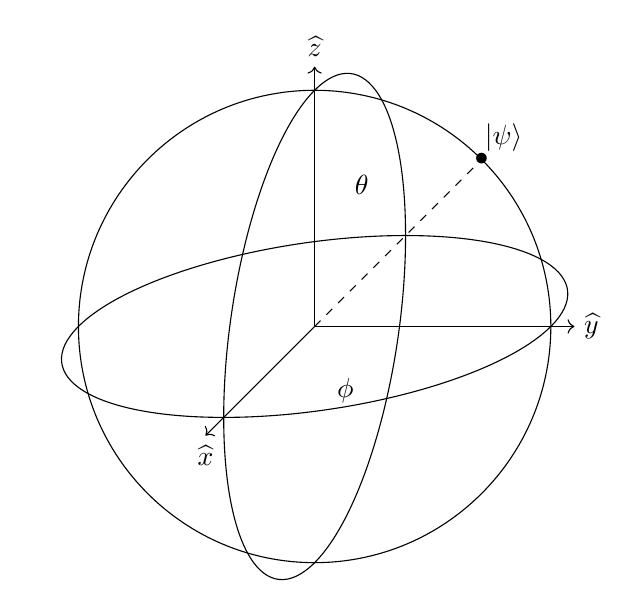
\begin{tikzpicture}[scale=3]
   \begin{scope}[canvas is zy plane at x=0]
     \draw (0,0) circle (1cm);
     %\draw[ultra thin] (-1,0) -- (1,0) (0,-1) -- (0,1);
     \draw[->] (0,0) -- (1.2,0) node[below] {$\widehat{x}$};
%     \draw (1.5,0) node {$\ket{+}$};  
%       \draw (-1.35,0) node {$\ket{-}$};
         
   \end{scope}

   \begin{scope}[canvas is zx plane at y=0]
     \draw (0,0) circle (1cm);
     %\draw (-1,0) -- (1,0) (0,-1) -- (0,1);
     \draw[->] (0,0) -- (0,1.1) node[right] {$\widehat{y}$};
        \centerarc[thick,->](0,0)(0:85:0.5)
	 \draw (0.70, 0.4) node {$\phi$};        
   \end{scope}

   \begin{scope}[canvas is xy plane at z=0]
     \draw (0,0) circle (1cm);
	%\draw (-1,0) -- (1,0) (0,-1) -- (0,1);
	\draw[->] (0,0) -- (0,1.1) node[above] {$\widehat{z}$};

     \draw[dashed] (0,0) -- (0.707,0.707) node {$\bullet$};
     \draw(0.8,0.8) node {$\ket{\psi}$};     
     	         \centerarc[thick,->](0,0)(90:45:0.5) 	
	 \draw (0.2, 0.6) node {$\theta$};
   \end{scope}
 \end{tikzpicture}
 \[
 \ket{\psi} & \simeq \cos(\half\theta)\ket{0} +e^{i\phi}\sin(\half\theta)\ket{1}
 \notag
 \\
 \notag
 {\widehat {n}}& =(\sin \theta \cos \phi ,\;\sin \theta \sin \phi ,\;\cos \theta )
 \]
 \end{center}
\caption{Bloch sphere representation of single qubit states.}
\end{figure}

Ultimately, a qubit  is a physical system with two distinct states, which we conventionally label zero and one. The state of the qubit $\ket{\psi}$ can be written as a superposition of zero states $\ket{0}$, and one states $\ket{1}$.
\[
\ket{\psi} = a \ket{0} + b \ket{1}, \qquad |a|^2 + |b|^2 = 1 
\]
where the coefficients $a$ and $b$ are complex numbers. We can rewrite this as
\[
\ket{\psi} =& e^{i\alpha} \left( \cos(\half\theta)\ket{0} +e^{i\phi}\sin(\half\theta)\ket{1}\right)
%\\ \notag
%\alpha &= 
%\\ \notag
%\theta &= 
%\\ \notag 
%\phi &=
\]
where $\alpha$, $\theta$, and $\phi$ are real numbers. The phase factor $e^{i\alpha}$ has no observable physical effect and can be ignored. It is merely an artifact of the mathematical representation. (If we use a density matrix representation then the phase factor disappears altogether.)
\[
\ket{\psi} \simeq \cos(\half\theta)\ket{0} +e^{i\phi}\sin(\half\theta)\ket{1}
\]
We'll use $\simeq$ to indicate that two states (or gates) are equal up to a phase factor.  
\index{$\simeq$, equal up to global phase}
\index{phase}

The parameters $\theta$ and $\phi$, can be interpreted as spherical coordinates of a point on the surface of a unit sphere, where $\theta$ is the colatitude with respect to the \axis{z}-axis and $\phi$ the longitude with respect to the \axis{x}-axis, and $0 \leq \theta \leq \pi$ and $0 \leq \phi < 2 \pi$. 
%
In cartesian coordinates the point on the 3-dimensional unit sphere is given by the Bloch vector \index{Bloch vector}
${\widehat {n}}=(\sin \theta \cos \phi ,\;\sin \theta \sin \phi ,\;\cos \theta )$.

% Check leq pi ?

\index{computational basis}
\index{computational basis|see{Z basis}}
\index{standard basis}
\index{standard basis|see{Z basis}}
\index{Hadamard basis}
\index{Hadamard basis|see{X basis}}
\index{X basis}
\index{Y basis}
\index{Z basis}
%
Note that the zero state, by convention, is located at the top of the Bloch sphere, and the one state at the bottom. 
States on opposite sides of the sphere are orthogonal, and any pair of such states provides a basis in which any state of a qubit can be represented. The other basis states located along the cartesian axes are common enough to have notation of their own. 
\[
\text{X basis} & &  \ket{+} & =\tfrac{1}{\sqrt{2}}(\ket{0}+\ket{1}) & \widehat{n}&=(+1,0,0) \notag\\
& & \ket{-} & =\tfrac{1}{\sqrt{2}}(\ket{0}-\ket{1})  & \widehat{n} &=(-1,0,0) \notag\\
\text{Y basis} & & \ket{+i} &=\tfrac{1}{\sqrt{2}}(\ket{0}+i\ket{1}) & \widehat{n}&=(0,+1,0) \notag\\
& & \ket{-i} &=\tfrac{1}{\sqrt{2}}(\ket{0}-i\ket{1}) & \widehat{n}&=(0,-1,0) \notag \\
\text{Z basis} & & \ket{0} & & \widehat{n}&=(0,0,+1) \notag\\
& & \ket{1} & & \widehat{n}&=(0,0,-1) \notag
\]
Generically we'll call these the X, Y, and Z bases.
The Z-basis is also called the computational or standard basis, is the one we label with zero and ones, and is generally the only basis in which we can make measurements of the system.  The X-basis is also called the Hadamard basis, since it can be generated from the computational basis with a Hadamard transform~\secref{sec:Hadamard}.
%
\index{$\ket{+}$}\index{$\ket{-}$}\index{$\ket{0}$}\index{$\ket{1}$}\index{$\ket{+i}$}\index{$\ket{-i}$}

% TODO: Explain other bases, give examples


Unfortunately, there aren't any real-space geometric representations of multi-qubit systems. The geometric representation of 1-qubit states by the Bloch sphere only works because of a mathematical accident that doesn't generalize.
# ~\pageref{accidental}.


\begin{figure}[tp]
\begin{center}
 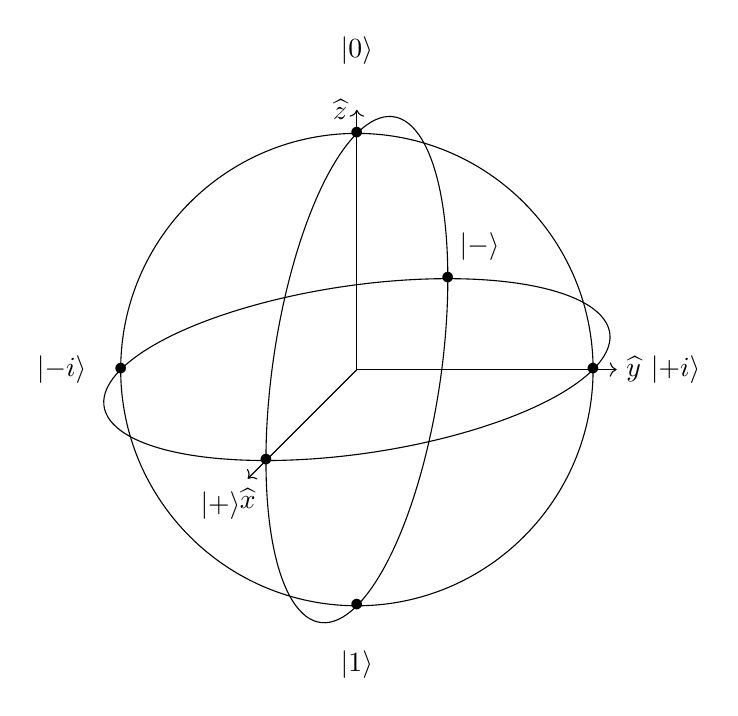
\begin{tikzpicture}[scale=3]
   \begin{scope}[canvas is zy plane at x=0]
     \draw (0,0) circle (1cm);
     %\draw[ultra thin] (-1,0) -- (1,0) (0,-1) -- (0,1);
     \draw[->] (0,0) -- (1.2,0) node[below] {$\widehat{x}$};
     \draw (1.5,0) node {$\ket{+}$};  
       \draw (-1.35,0) node {$\ket{-}$};
         	 \draw (1, 0) node {$\bullet$};        
	 \draw (-1, 0) node {$\bullet$};
   \end{scope}

   \begin{scope}[canvas is zx plane at y=0]
     \draw (0,0) circle (1cm);
     %\draw (-1,0) -- (1,0) (0,-1) -- (0,1);
     \draw[->] (0,0) -- (0,1.1) node[right] {$\widehat{y}$};
	 \draw (0, 1) node {$\bullet$};        
	 \draw (0, -1) node {$\bullet$}; 
	  	\draw (0,1.35) node {$\ket{+i}$};
	\draw (0,-1.25) node {$\ket{-i}$};
   \end{scope}

   \begin{scope}[canvas is xy plane at z=0]
     \draw (0,0) circle (1cm);
	%\draw (-1,0) -- (1,0) (0,-1) -- (0,1);
	\draw[->] (0,0) -- (0,1.1) node[left] {$\widehat{z}$};
	 \draw (0, 1) node {$\bullet$};        
	 \draw (0, -1) node {$\bullet$};
	\draw (0,1.35) node {$\ket{0}$};
	\draw (0,-1.25) node {$\ket{1}$};	 
   \end{scope}
 \end{tikzpicture}
 \end{center}
\caption{Location of standard basis states on the Bloch sphere.}
\end{figure}




% !TEX encoding = UTF-8 Unicode 
% !TEX root = on_gates.tex



\clearpage
\section{Standard 1-qubit gates}
% TODO: Define "standard" gates


Classically, there are only 2 1-bit reversible logic gates, identity and NOT (And 2 irreversible gates, reset to 0 and reset to 1). But in quantum mechanics the zero and one states can be placed into superposition, so there are many other interesting possibilities. 

\subsection{Pauli gates}
\index{Pauli gates}
\index{Pauli gates!commutation relations}
The simplest 1-qubit gates are the 4 gates represented by the Pauli operators, I, X, Y, and Z. These operators are also sometimes notated as $\sigma_x$, $\sigma_y$, $\sigma_z$, or with an index $\sigma_i$, so that $\sigma_0=I$, $\sigma_1=X$, $\sigma_2=Y$, $\sigma_3=Z$. % Move to section on pauli group
\index{$\sigma_x$}\index{$\sigma_y$}\index{$\sigma_z$}

We will explore the algebra of Pauli operators in more detail in chapter~\secref{sec:pauli}. But for now, note that the Pauli gates are all Hermitian, $\sigma_i^\dagger=\sigma_i$, square to the identity $\sigma_i^2 =I$, and that the $X$, $Y$, and $Z$ gates anti-commute with each other.
\[
XY = -YZ = iZ \notag \\
YZ = -ZY = iX \notag \\
ZX = -ZX = iY \notag \\
XYZ = iI \notag
\]


\paragraph{Pauli-I gate} (identity):\index{identity gate! 1-qubit}
\index{I gate@\Gate{I} gate|see {identity gate}}
\[
I = \begin{bmatrix}1 & 0 \\ 0 & 1 \end{bmatrix}
\]
\begin{center}
\adjustbox{scale=0.8}{\begin{quantikz}[thin lines, column sep=0.75em,row sep={2.5em,between origins}]
& \gate{I} & \qw
\end{quantikz}
}
\end{center}
The trivial no-operation gate on 1-qubit, represented by the identity matrix. Acting on any arbitrary state, the gate leave the state unchanged.%
%
%\begin{center}
%\adjustbox{scale=0.75}{
% \begin{tikzpicture}[scale=1.5]
%   \begin{scope}[canvas is zy plane at x=0]
%     \draw (0,0) circle (1cm);
%     %\draw[ultra thin] (-1,0) -- (1,0) (0,-1) -- (0,1);
%     \draw[->] (0,0) -- (1.35,0) node[below] {$\widehat{x}$};
%%     \draw[dashed] (0,0) -- (1.,1.) ;
%   \end{scope}
%
%   \begin{scope}[canvas is zx plane at y=0]
%     \draw (0,0) circle (1cm);
%     %\draw (-1,0) -- (1,0) (0,-1) -- (0,1);
%     \draw[->] (0,0) -- (0,1.175) node[right] {$\widehat{y}$};
%   \end{scope}
%
%   \begin{scope}[canvas is xy plane at z=0]
%     \draw (0,0) circle (1cm);
%	%\draw (-1,0) -- (1,0) (0,-1) -- (0,1);
%	\draw[->] (0,0) -- (0,1.175) node[above] {$\widehat{z}$};
%   \end{scope}
%
%%   \begin{scope}[canvas is zx plane at y=1.0]	
%%   	\centerarc[blue,->](0,0)(270:90:0.25)
%%   \end{scope}
%    
%   \draw[->] (1.5,0) -- node[above] {$I$} ++(0.5, 0) ;
%
%	\begin{scope}[xshift=3.5cm]
%    \begin{scope}[canvas is zy plane at x=0]
%     \draw (0,0) circle (1cm);
%     %\draw[ultra thin] (-1,0) -- (1,0) (0,-1) -- (0,1);
%     \draw[->] (0,0) -- (1.35,0) node[below] {$\widehat{x}$};
%%     \draw[dashed] (0,0) -- (1.,1.) ;
%   \end{scope}
%
%   \begin{scope}[canvas is zx plane at y=0]
%     \draw (0,0) circle (1cm);
%     %\draw (-1,0) -- (1,0) (0,-1) -- (0,1);
%     \draw[->] (0,0) -- (0,1.175) node[right] {$\widehat{y}$};
%   \end{scope}
%
%   \begin{scope}[canvas is xy plane at z=0]
%     \draw (0,0) circle (1cm);
%	%\draw (-1,0) -- (1,0) (0,-1) -- (0,1);
%	\draw[->] (0,0) -- (0,1.175) node[above] {$\widehat{z}$};
%   \end{scope}
%
%\end{scope}
% \end{tikzpicture}
%}
% \end{center}
%
%
\[
I &=\ket{0}\!\bra{0} + \ket{1}\!\bra{1} \notag \\
I&\ket{0} = \ket{0} \notag \\ 
I&\ket{1} = \ket{1} \notag
\]




\paragraph{Pauli-X gate} (X gate, bit flip) %, NOT, bit flip, negation) \cite{Barenco1995b}
\index{Pauli-X gate}
\index{X@$\Gate{X}$|see {Pauli-X gate}}
\index{bit flip|see {Pauli-X gate}}
\[
X = \begin{bmatrix}0 & 1 \\ 1 & 0 \end{bmatrix}
\]
\begin{center}
\adjustbox{scale=0.8}{\begin{quantikz}[thin lines, column sep=0.75em,row sep={2.5em,between origins}]
& \gate{X} & \qw
\end{quantikz}
}
\end{center}


The $X$-gate generates a half-turn in the Bloch sphere about the $x$ axis. 
%
\begin{center}
\adjustbox{scale=0.75}{
 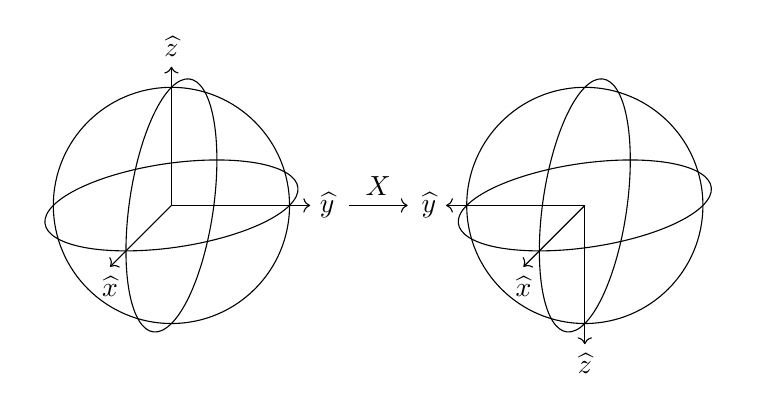
\begin{tikzpicture}[scale=1.5]
   \begin{scope}[canvas is zy plane at x=0]
     \draw (0,0) circle (1cm);
     %\draw[ultra thin] (-1,0) -- (1,0) (0,-1) -- (0,1);
     \draw[->] (0,0) -- (1.35,0) node[below] {$\widehat{x}$};
%     \draw[dashed] (0,0) -- (1.,1.) ;
   \end{scope}

   \begin{scope}[canvas is zx plane at y=0]
     \draw (0,0) circle (1cm);
     %\draw (-1,0) -- (1,0) (0,-1) -- (0,1);
     \draw[->] (0,0) -- (0,1.175) node[right] {$\widehat{y}$};
   \end{scope}

   \begin{scope}[canvas is xy plane at z=0]
     \draw (0,0) circle (1cm);
	%\draw (-1,0) -- (1,0) (0,-1) -- (0,1);
	\draw[->] (0,0) -- (0,1.175) node[above] {$\widehat{z}$};
   \end{scope}

%   \begin{scope}[canvas is zx plane at y=1.0]	
%   	\centerarc[blue,->](0,0)(270:90:0.25)
%   \end{scope}
    
   \draw[->] (1.5,0) -- node[above] {$X$} ++(0.5, 0) ;

	\begin{scope}[xshift=3.5cm]
    \begin{scope}[canvas is zy plane at x=0]
     \draw (0,0) circle (1cm);
     %\draw[ultra thin] (-1,0) -- (1,0) (0,-1) -- (0,1);
     \draw[->] (0,0) -- (1.35,0) node[below] {$\widehat{x}$};
%     \draw[dashed] (0,0) -- (1.,1.) ;
   \end{scope}

   \begin{scope}[canvas is zx plane at y=0]
     \draw (0,0) circle (1cm);
     %\draw (-1,0) -- (1,0) (0,-1) -- (0,1);
     \draw[->] (0,0) -- (0,-1.175) node[left] {$\widehat{y}$};
   \end{scope}

   \begin{scope}[canvas is xy plane at z=0]
     \draw (0,0) circle (1cm);
	%\draw (-1,0) -- (1,0) (0,-1) -- (0,1);
	\draw[->] (0,0) -- (0,-1.175) node[below] {$\widehat{z}$};
   \end{scope}

\end{scope}
 \end{tikzpicture}
}
 \end{center}


With respect to the computational basis, the $X$ gate is equivalent to a classical NOT operation, or logical negation. The computation basis states are interchanged, so that $\ket{0}$ becomes $\ket{1}$ and $\ket{1}$ becomes $\ket{0}$.
\index{NOT gate}\index{logical negation}
\[
X &=\ket{1}\!\bra{0} + \ket{0}\!\bra{1} \notag \\
X&\ket{0} = \ket{1} \notag \\ 
X&\ket{1} = \ket{0} \notag
\]
However, the X-gate is not a true quantum NOT gate, since it only logically negates the state in the computational basis. A true quantum logical negation would require mapping every point on the Bloch sphere to its antipodal point. But that would require an inversion of the sphere which cannot be generated by rotations alone. There is no general quantum NOT operation that would negate an arbitrary qubit state.


\paragraph{Pauli-Y gate} (Y-gate):
\index{Pauli-Y gate}
\index{Y gate@\Gate{Y} gate|see {Pauli-Y gate}}
\[
Y = \begin{bmatrix*}[r]0 & -i \\ i & 0 \end{bmatrix*}
\]
\begin{center}
\adjustbox{scale=0.8}{\begin{quantikz}[thin lines, column sep=0.75em,row sep={2.5em,between origins}]
& \gate{Y} & \qw
\end{quantikz}
}
\end{center}
A useful mnemonic for remembering where to place the minus sign in the matrix of the Y gate is ``Minus eye high''~\cite{???}. \index{minus eye high}
% TODO: What's the origin of this?
In some older literature the Y-gate is defined as $iY=\begin{bsmallmatrix} 0 & 1 \\ -1 & 0 \end{bsmallmatrix}$ (e.g.~\cite{Rieffel2014a}), which is the same gate up to a phase.


The Pauli-Y gate generates a half-turn in the Bloch sphere about the $\widehat{y}$ axis.
\begin{center}
\adjustbox{scale=0.75}{
 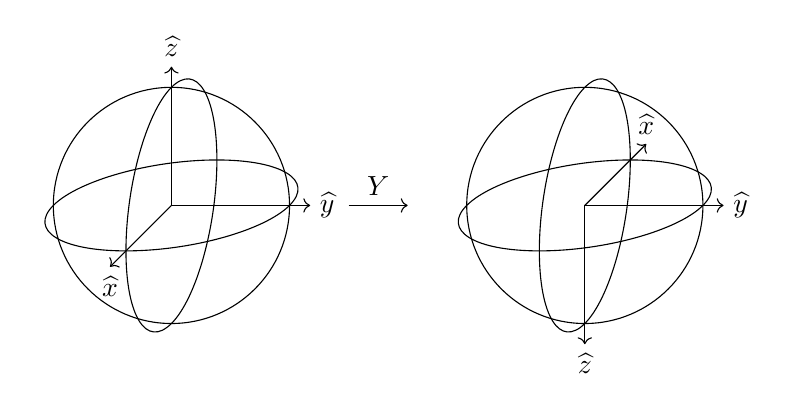
\begin{tikzpicture}[scale=1.5]
   \begin{scope}[canvas is zy plane at x=0]
     \draw (0,0) circle (1cm);
     %\draw[ultra thin] (-1,0) -- (1,0) (0,-1) -- (0,1);
     \draw[->] (0,0) -- (1.35,0) node[below] {$\widehat{x}$};
%     \draw[dashed] (0,0) -- (1.,1.) ;
   \end{scope}

   \begin{scope}[canvas is zx plane at y=0]
     \draw (0,0) circle (1cm);
     %\draw (-1,0) -- (1,0) (0,-1) -- (0,1);
     \draw[->] (0,0) -- (0,1.175) node[right] {$\widehat{y}$};
   \end{scope}

   \begin{scope}[canvas is xy plane at z=0]
     \draw (0,0) circle (1cm);
	%\draw (-1,0) -- (1,0) (0,-1) -- (0,1);
	\draw[->] (0,0) -- (0,1.175) node[above] {$\widehat{z}$};
   \end{scope}

%   \begin{scope}[canvas is zx plane at y=1.0]	
%   	\centerarc[blue,->](0,0)(270:90:0.25)
%   \end{scope}
    
   \draw[->] (1.5,0) -- node[above] {$Y$} ++(0.5, 0) ;

	\begin{scope}[xshift=3.5cm]
    \begin{scope}[canvas is zy plane at x=0]
     \draw (0,0) circle (1cm);
     %\draw[ultra thin] (-1,0) -- (1,0) (0,-1) -- (0,1);
     \draw[->] (0,0) -- (-1.35,0) node[above] {$\widehat{x}$};
%     \draw[dashed] (0,0) -- (1.,1.) ;
   \end{scope}

   \begin{scope}[canvas is zx plane at y=0]
     \draw (0,0) circle (1cm);
     %\draw (-1,0) -- (1,0) (0,-1) -- (0,1);
     \draw[->] (0,0) -- (0,1.175) node[right] {$\widehat{y}$};
   \end{scope}

   \begin{scope}[canvas is xy plane at z=0]
     \draw (0,0) circle (1cm);
	%\draw (-1,0) -- (1,0) (0,-1) -- (0,1);
	\draw[->] (0,0) -- (0,-1.175) node[below] {$\widehat{z}$};
   \end{scope}

\end{scope}
 \end{tikzpicture}
}
 \end{center}

The $Y$-gate can be thought of as a combination of $X$ and $Z$ gates, $Y=-iZX$. With respect to the computational basis, we interchange the zero and one states and apply a relative phase flip.
\[
Y & =i\ket{1}\!\bra{0} -i \ket{0}\!\bra{1} \notag\\
Y & \ket{0} = +i\ket{1} \notag \\ 
Y & \ket{1} = -i\ket{0} \notag
\]




\paragraph{Pauli-Z gate} (Z-gate, phase flip)%
\index{Pauli-Z gate}%
\index{phase flip|see {Pauli-Z gate}}%
\index{Z gate|see {Pauli-Z gate}}
\[
Z = \begin{bmatrix*}[r]1 & 0 \\ 0 & -1 \end{bmatrix*}
\]
\begin{center}
\adjustbox{scale=0.8}{\begin{quantikz}[thin lines, column sep=0.75em,row sep={2.5em,between origins}]
& \gate{Z} & \qw
\end{quantikz}
}
\end{center}
\[
H_Z = - \pi\half(1 - Z)
\notag
\]


The Pauli-Z gate generates a half-turn in the Bloch sphere about the $\widehat{z}$ axis.
\begin{center}
\adjustbox{scale=0.75}{
 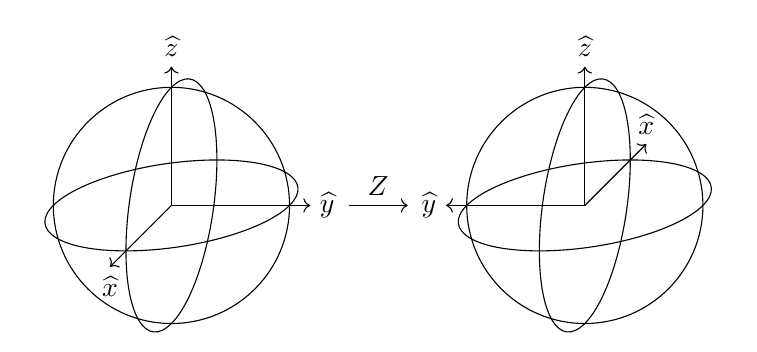
\begin{tikzpicture}[scale=1.5]
   \begin{scope}[canvas is zy plane at x=0]
     \draw (0,0) circle (1cm);
     %\draw[ultra thin] (-1,0) -- (1,0) (0,-1) -- (0,1);
     \draw[->] (0,0) -- (1.35,0) node[below] {$\widehat{x}$};
%     \draw[dashed] (0,0) -- (1.,1.) ;
   \end{scope}

   \begin{scope}[canvas is zx plane at y=0]
     \draw (0,0) circle (1cm);
     %\draw (-1,0) -- (1,0) (0,-1) -- (0,1);
     \draw[->] (0,0) -- (0,1.175) node[right] {$\widehat{y}$};
   \end{scope}

   \begin{scope}[canvas is xy plane at z=0]
     \draw (0,0) circle (1cm);
	%\draw (-1,0) -- (1,0) (0,-1) -- (0,1);
	\draw[->] (0,0) -- (0,1.175) node[above] {$\widehat{z}$};
   \end{scope}

%   \begin{scope}[canvas is zx plane at y=1.0]	
%   	\centerarc[blue,->](0,0)(270:90:0.25)
%   \end{scope}
    
   \draw[->] (1.5,0) -- node[above] {$Z$} ++(0.5, 0) ;

	\begin{scope}[xshift=3.5cm]
   \begin{scope}[canvas is zy plane at x=0]
     \draw (0,0) circle (1cm);
     %\draw[ultra thin] (-1,0) -- (1,0) (0,-1) -- (0,1);
     \draw[->] (0,0) -- (-1.35,0) node[above] {$\widehat{x}$};
   \end{scope}

   \begin{scope}[canvas is zx plane at y=0]
     \draw (0,0) circle (1cm);
     %\draw (-1,0) -- (1,0) (0,-1) -- (0,1);
     \draw[->] (0,0) -- (0,-1.175) node[left] {$\widehat{y}$};
   \end{scope}

   \begin{scope}[canvas is xy plane at z=0]
     \draw (0,0) circle (1cm);
	%\draw (-1,0) -- (1,0) (0,-1) -- (0,1);
	\draw[->] (0,0) -- (0,1.175) node[above] {$\widehat{z}$};
   \end{scope}
	\end{scope}


 \end{tikzpicture}
}
 \end{center}

With respect to the computational basis, the $Z$ gate flips the phase of the $\ket{1}$ state relative to the $\ket{0}$ state.
\[
Z &=\ket{0}\!\bra{0} - \ket{1}\!\bra{1} \notag\\
Z& \ket{0}  = +\ket{0} \notag \\ 
Z&\ket{1} = -\ket{1} \notag
\]

\todo{ Comment on Z gate}

% Pauli gates are all Hermitian



\subsection{Rotation gates}\index{Rotation gates}
The three Pauli-rotation gates\endnote{The 1-qubit rotation gates are typically verbalized as {\sl arr-ex}, {\sl arr-why}, {\sl arr-zee}, and {\sl arr-en}.\index{quantum pirate gates}} $R_x$, $R_y$, and $R_z$ rotate the state vector by an arbitrary angle about the corresponding axis in the Bloch sphere, Fig.~\ref{fig:paulirotations}. They are generated by taking exponentials of the Pauli operators. 
\todo{Wordsmith} 

A useful identity to keep in mind is that given an operator~$A$ that squares to the identity $A^2=I$ then
\[
\exp(i\theta A) = \cos(\theta)\ I + i \sin(\theta)\ A
\]
This is a generalization of the usual Euler's formula $e^{ix} =\cos x + i \sin x$. We expand the exponential as a power series, and gather the even powers into the cosine term, and the odd powers into the sin term.
\[
\exp(i\theta A) & = I + i \theta A - \tfrac{\theta^2}{2!} I - i \tfrac{\theta^3}{3!} A 
- \tfrac{\theta^4}{4!} I - i \tfrac{\theta^5}{5!} A +
+ \cdots \notag \\
& = \left(1- \tfrac{\theta^2}{2!} +\tfrac{\theta^4}{4!} - \cdots\right) I +  
    \left(\theta -\tfrac{\theta^3}{3!} +\tfrac{\theta^5}{5!}- \cdots\right)A
    \notag
    \\ \notag
 & = \cos(\theta)\ I + i \sin(\theta)\ A
\]


\paragraph{$R_x$ gate}\cite{Barenco1995b}\index{Rx gate@\Gate{R_x} gate} Rotate $\theta$ radians anti-clockwise about the \axis{x} axis of the Bloch sphere.
\[
        R_x(\theta) & =  e^{-i \half\theta X} 
        			\\ \notag & = \cos(\half\theta) I -i \sin(\half\theta) X		
\\ \notag
			 &= \begin{bmatrix*}[r]
                            \cos(\half\theta) & -i \sin(\half\theta) \\
                            -i \sin(\half\theta) & \cos(\half\theta)
                        \end{bmatrix*}                        
\\ \notag
    H_{R_x} & = \half\theta X 
    \]

The $R_x$ gate is represented by the following circuit diagram.
$$
\adjustbox{scale=0.8}{\begin{quantikz}[thin lines, column sep=0.75em,row sep={2.5em,between origins}]
& \gate{R_x(\theta)} & \qw
\end{quantikz}
}
$$
or, if we want to specify a generic $R_x$ gate, and not a specific angle, we can drop the theta argument.
$$
\adjustbox{scale=0.8}{\begin{quantikz}[thin lines, column sep=0.75em,row sep={2.5em,between origins}]
& \gate{R_x} & \qw
\end{quantikz}
}
$$

\paragraph{$R_y$ gate}\cite{Barenco1995b}\index{Ry gate@\Gate{R_y} gate} Rotate $\theta$ radians anti-clockwise about the $\widehat{y}$ axis of the Bloch sphere.
\[
        R_y(\theta) 
        & =  e^{-i \half\theta Y} 
        			\\ \notag &  = \cos(\half\theta) I -i \sin(\half\theta) Y		
\\ \notag
			 &=
           \begin{bmatrix*}[r]
 			\cos(\half\theta) & -\sin(\half\theta)
        	\\ \sin(\half\theta) & \cos(\half\theta)
                        \end{bmatrix*}
\]
$$
\adjustbox{scale=0.8}{\begin{quantikz}[thin lines, column sep=0.75em,row sep={2.5em,between origins}]
& \gate{R_y(\theta)} & \qw
\end{quantikz}
}
$$
    \[
    \notag
    H_{R_y} & = \half\theta Y
    \]




\paragraph{$R_z$ gate}\cite{Barenco1995b}\index{Rz gate@\Gate{R_z} gate}
Rotate $\theta$ radians anti-clockwise about the $\widehat{z}$ axis of the Bloch sphere.

\[
        R_z(\theta) 
        & =  e^{-i \half\theta Z} 
        			\\ \notag & = \cos(\half\theta) I -i \sin(\half\theta) Z		
\\ \notag
			 &=
           \begin{bmatrix*}
        e^{-i\half\theta} & 0 \\
        0 & e^{+i\half\theta}
                        \end{bmatrix*}
\]
$$
\adjustbox{scale=0.8}{\begin{quantikz}[thin lines, column sep=0.75em,row sep={2.5em,between origins}]
& \gate{R_z(\theta)} & \qw
\end{quantikz}
}
$$
    \[
    \notag
    H_{R_z} & = \half\theta Z 
    \]

% TODO: Comment on being diagonal?


Consecutive rotations about the same axis can be merged, with the total angle being the sum of angles.
$$
\adjustbox{scale=0.8}{\begin{quantikz}[thin lines, column sep=0.75em,row sep={2.5em,between origins}]
& \gate{R_x(\theta_{0})} & \gate{R_x(\theta_{1})} & \qw
\end{quantikz}
} = \adjustbox{scale=0.8}{\begin{quantikz}[thin lines, column sep=0.75em,row sep={2.5em,between origins}]
& \gate{R_x(\theta_{0}+\theta_{1})} & \qw
\end{quantikz}
}
$$
$$
\adjustbox{scale=0.8}{\begin{quantikz}[thin lines, column sep=0.75em,row sep={2.5em,between origins}]
& \gate{R_y(\theta_{0})} & \gate{R_y(\theta_{1})} & \qw
\end{quantikz}
} = \adjustbox{scale=0.8}{\begin{quantikz}[thin lines, column sep=0.75em,row sep={2.5em,between origins}]
& \gate{R_y(\theta_{0}+\theta_{1})} & \qw
\end{quantikz}
}
$$
$$
\adjustbox{scale=0.8}{\begin{quantikz}[thin lines, column sep=0.75em,row sep={2.5em,between origins}]
& \gate{R_z(\theta_{0})} & \gate{R_z(\theta_{1})} & \qw
\end{quantikz}
} = \input{circuits/Rz01}
$$



Let us demonstrate that the $R_z$ gate generates rotations about the $\widehat{z}$ axis. Recall the definition of the Bloch vector of an arbitrary state $\ket{\psi}$, \secref{sec:blochsphere}.
\[
R_z(\theta') \ket{\psi} &= 
	\Bigl(e^{-i\half\theta'} \ket{0}\!\bra{0} + e^{+i\half\theta'} \ket{1}\!\bra{1}\Bigr)
	\Bigl( \cos(\half\theta)\ket{0} +e^{i\phi}\sin(\half\theta)\ket{1}\Bigr)
\notag
\\
\notag 
& = e^{-i\half\theta'} \Bigl( cos(\half\theta)\ket{0} + e^{i(\theta'+\phi)} \ket{1}\Bigr)
\\ 
& \simeq cos(\half\theta)\ket{0} + e^{i(\theta'+\phi)}\ket{1}
\]
In the last line we drop an irrelevant phase. We can see that the $R_z$ gate has left the elevation angle unchanged, but added $\theta'$ to the azimuth angle, which corresponds to a rotation about the \axis{z}-axis. 

We can do the same exercise for the $R_X$ and $R_Y$ gates, although the trigonometry is slightly more involved.

%TODO: R_X or R_x?

\begin{figure}[t]
\begin{center}
%\adjustbox{scale=0.75}{
 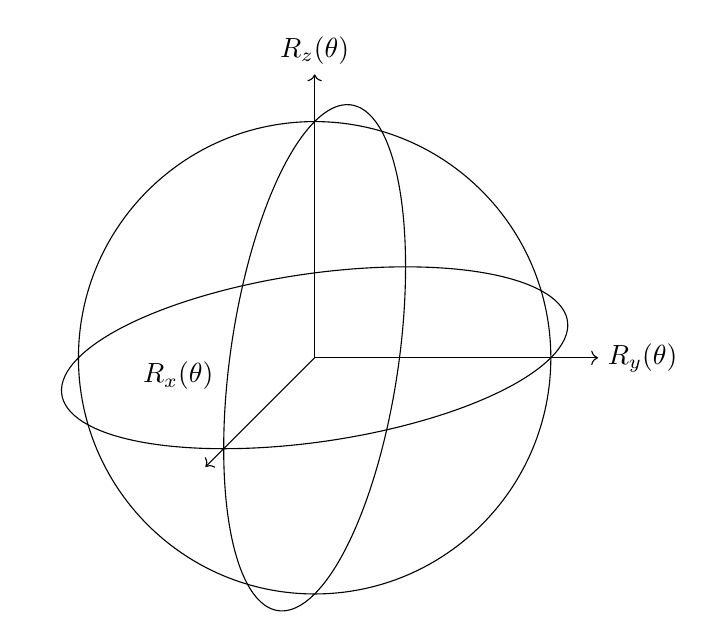
\begin{tikzpicture}[scale=3]
   \begin{scope}[canvas is zy plane at x=0]
     \draw (0,0) circle (1cm);
     %\draw[ultra thin] (-1,0) -- (1,0) (0,-1) -- (0,1);
     \draw[->] (0,0) -- (1.2,0); 
     \draw (1.5, 0.5) node {$R_x(\theta)$};
   \end{scope}

   \begin{scope}[canvas is zx plane at y=0]
     \draw (0,0) circle (1cm);
     %\draw (-1,0) -- (1,0) (0,-1) -- (0,1);
     \draw[->] (0,0) -- (0,1.2) node[right] {$R_y(\theta)$};
   \end{scope}

   \begin{scope}[canvas is xy plane at z=0]
     \draw (0,0) circle (1cm);
	\draw[->] (0,0) -- (0,1.2) node[above] {$R_z(\theta)$};
	\end{scope}
		 
   \begin{scope}[canvas is xy plane at z=1.0]	
   	\centerarc[thick,blue, ->](0,0)(-135:450:0.25)
   \end{scope}

   \begin{scope}[canvas is zy plane at x=1.0]	
   	\centerarc[thick,blue, ->](0,0)(450:-135:0.25)
   \end{scope}

   \begin{scope}[canvas is zx plane at y=1.00]	
   	\centerarc[thick,blue, ->](0,0)(-135:450:0.25)
   \end{scope}
 \end{tikzpicture}
%    }
 \end{center}
\caption{Pauli rotations of the Bloch Sphere}
\label{fig:paulirotations}
\end{figure}



\paragraph{$R_{\vec{n}}$ gate} \index{Rn gate@$R_{\vec{n}}$ gate|see {rotation gate}}\index{rotation gate}
A rotation of $\theta$ radians anti-clockwise about an arbitrary axis in the Bloch sphere.
\[
\label{Rn}
R_{\vec{n}}(\theta) &
=  e^{-i\half \theta (n_x X+ n_y Y + n_z Z)}
\\ 
\notag
&= \cos(\half\theta) I - i \sin(\half\theta)(n_x X+ n_y Y + n_z Z)
\\
& = \notag
\begin{bmatrix*}
	\cos(\half\theta) - i n_z \sin(\half\theta)  &
	- n_y \sin(\half\theta)-i n_x \sin(\half\theta)  \\
	n_y \sin(\half\theta)-i n_x \sin(\half\theta)   & 
	\cos(\half\theta) + i n_z \sin(\half\theta)
\end{bmatrix*}
\]
\begin{center}
\adjustbox{scale=0.9}{\begin{quantikz}[thin lines, column sep=0.75em, row sep={2.5em,between origins}]
& \gate{R_{\vec{n}}(\theta)} & \qw
\end{quantikz}
}
\end{center}
Every 1-qubit gate can be represented as a rotation gate (up to phase) 
with some coordinate $(\theta\ n_x, \theta\ n_y, \theta\ n_z)$, where $n_x^2 +n_y^2 +n_z^2 =1$ and $\theta$ runs between $\pi$ and $-\pi$.
The Pauli gates are the rotations around the principal axes.
\[
R_x(\theta) & = R_{\vec{n}}(\theta), \quad \vec{n} = (1, 0, 0) \notag \\
R_y(\theta) & = R_{\vec{n}}(\theta), \quad \vec{n} = (0, 1, 0) \notag \\
R_z(\theta) & = R_{\vec{n}}(\theta), \quad \vec{n} = (0, 0, 1) \notag
\]
This representation provides a convenient visualization of 1-qubit gates: The 1-qubit gates form a spherical ball of radius $\theta$.  See figures~\ref{fig:sphere-of-gates} and~\ref{fig:GateCoords}. This sphere-of-gates is distinct from the Bloch sphere of states, although the underlying mathematical structures are related.

% TODO: Merging rotations


You might reasonably be wondering why there is a factor of half in the definitions of the rotation gates. A 1-qubit gate is represented by an element of the group $SU(2)$ (the group of $2\times2$ unitary matrices with unit determinate). Each element is a rotation in a 2-dimensional complex vector space. But we are visualizing the effect of these gates as rotations in 3-dimensional Euclidean space, which are elements of the special orthogonal group $SO(3)$. We can do this because there is an accidental correspondence between these two groups that allows us to visualize 1-qubit gates as rotations in 3-space. We can map two elements of $SU(2)$ (differing by only a -1 phase) to each element of $SO(3)$ while keeping the group structure. In the jargon, $SU(2)$ is a double cover of $SO(3)$. Because of this doubling up, a rotation of $\theta$ radians in the Bloch sphere corresponds to a rotation of only $\half \theta$ in the complex vector space. We have to go twice around the Bloch sphere, $\theta =4\pi$, to get back to the same gate with the same phase.


\todo{Check double cover nomenclature}

% Hamiltonian of R_n?



%
%\begin{figure}[t]
%\begin{center}
% \begin{tikzpicture}[scale=3]
%   \begin{scope}[canvas is zy plane at x=0]
%     \draw (0,0) circle (1cm);
%     %\draw[ultra thin] (-1,0) -- (1,0) (0,-1) -- (0,1);
%     \draw[] (0,0) -- (1.2,0) node[below left] {$R_x(\theta)$};
%   \end{scope}
%
%   \begin{scope}[canvas is zx plane at y=0]
%     \draw (0,0) circle (1cm);
%     %\draw (-1,0) -- (1,0) (0,-1) -- (0,1);
%     \draw[] (0,0) -- (0,1.1) node[right] {$R_y(\theta)$};
%   \end{scope}
%
%   \begin{scope}[canvas is xy plane at z=0]
%     \draw (0,0) circle (1cm);
%	\draw[] (0,0) -- (0,1.1) node[above] {$R_z(\theta)$};
%	\end{scope}
%		 
%   \begin{scope}[canvas is xy plane at z=1.0]	
%   	\centerarc[red,->](0,0)(450:135:0.25)
%   \end{scope}
%
%   \begin{scope}[canvas is zy plane at x=1.0]	
%   	\centerarc[blue,<-](0,0)(450:135:0.25)
%   \end{scope}
%
%   \begin{scope}[canvas is zx plane at y=1.0]	
%   	\centerarc[green,->](0,0)(450:135:0.25)
%   \end{scope}
%
%	 
%	 
%	 
% \end{tikzpicture}
% \end{center}
%\caption{Rotations of the Bloch Sphere}
%\end{figure}
%

\begin{figure}[tp]
\begin{center}
 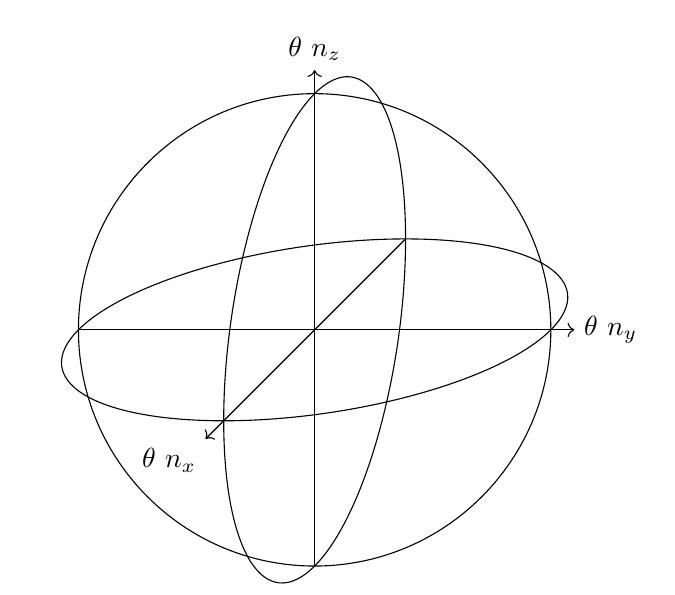
\begin{tikzpicture}[scale=3]
   \begin{scope}[canvas is zy plane at x=0]
     \draw (0,0) circle (1cm);
     %\draw[ultra thin] (-1,0) -- (1,0) (0,-1) -- (0,1);
     \draw[->] (-1,0) -- (1.2,0) node[below left] {$\theta\ n_x$};
   \end{scope}

   \begin{scope}[canvas is zx plane at y=0]
     \draw (0,0) circle (1cm);
     %\draw (-1,0) -- (1,0) (0,-1) -- (0,1);
     \draw[->] (0,-1) -- (0,1.1) node[right] {$\theta\ n_y$};
   \end{scope}

   \begin{scope}[canvas is xy plane at z=0]
     \draw (0,0) circle (1cm);
	%\draw (-1,0) -- (1,0) (0,-1) -- (0,1);
	\draw[->] (0,-1) -- (0,1.1) node[above] {$\theta\ n_z$};
   \end{scope}

	 
 \end{tikzpicture}
 \end{center}

\caption[Spherical ball of 1-qubit gates]{Spherical ball of 1-qubit gates \eqref{Rn}. Each point within this sphere represents a unique 1-qubit gate (up to phase). 
Antipodal points on the surface represent the same gate. The Pauli rotation gates lie along the three principal axes.}
 \label{fig:sphere-of-gates} 
%\end{figure}

%\begin{figure}[t]
\begin{center}
 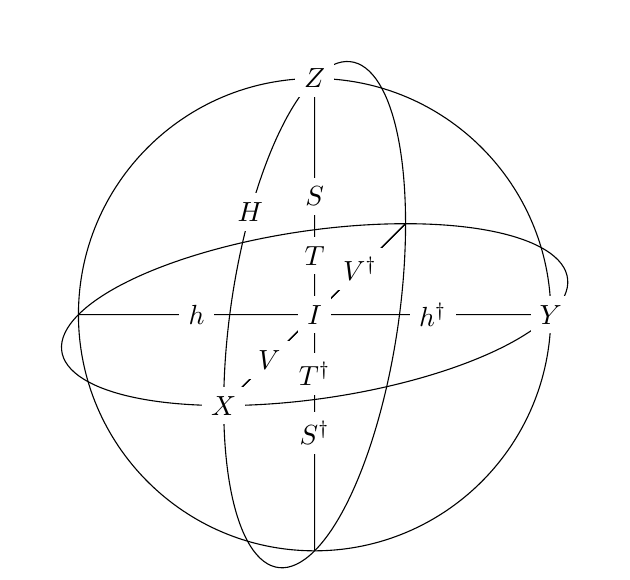
\begin{tikzpicture}[scale=3]
   \begin{scope}[canvas is zy plane at x=0]
     \draw (0,0) circle (1cm);
     \draw (-1,0) -- (1,0) (0,-1) -- (0,1);
   \end{scope}

   \begin{scope}[canvas is zx plane at y=0]
     \draw (0,0) circle (1cm);
     \draw (-1,0) -- (1,0) (0,-1) -- (0,1);
   \end{scope}

   \begin{scope}[canvas is xy plane at z=0]
     \draw (0,0) circle (1cm);
     \draw (-1,0) -- (1,0) (0,-1) -- (0,1);
   \end{scope}

	\node[fill=white] at (0,0,0) {$I$};

	\node[fill=white] at (0,1,0) {$Z$};
	\node[fill=white] at (0,0.5,0) {$S$};
	\node[fill=white] at (0,0.25,0) {$T$};			
	\node[fill=white] at (0,-0.5,0) {${S^\dagger}$};
	\node[fill=white] at (0,-0.25,0) {$T^\dagger$};	
	% \node[fill=white] at (0,-1,0) {Z};
		
	\node[fill=white] at (0,0,1) {$X$};
	\node[fill=white] at (0,0,0.5) {$V$};
	\node[fill=white] at (0,0,-0.5) {$V^\dagger$};	
	% \node[fill=white] at (0,0,-1) {X};
	
	\node[fill=white] at (0,{sqrt(1/2)},{sqrt(1/2)}) {$H$};
%	\node[fill=white] at (0,0,1) {H};
	
	\node[fill=white] at (1,0,0) {$Y$};
	\node[fill=white] at (0.5,0,0) {${h^\dagger}$};	
	\node[fill=white] at (-0.5,0,0) {${h}$};	
	% \node[fill=white] at (-1,0,0) {$Y$};
 \end{tikzpicture}
 \end{center}

\caption[Coordinates of common 1-qubit gates.]{Coordinates of common 1-qubit gates \eqref{Rn}.}
 \label{fig:GateCoords}
\end{figure}


\subsection{Pauli-power gates}\index{Pauli-power gates}
It turns out to be useful to define powers of the Pauli-gates. This is slightly tricky because non-integer powers of matrixes aren't unique. Just as there are 2-square roots of any number, a diagonalizable matrix with $n$ unique eigenvalue has $2^n$ unique square roots. We circumvent this ambiguity by defining the Pauli power gates via the Pauli rotation gates. We note that a $\pi$ rotation is a Pauli gate up to phase, e.g.
\[
R_{X}(\pi) = e^{-i \tfrac{\pi}{2}X } = -i X 
\]
and define powers of the Pauli matrices as 
\[
X^t =e^{-i \tfrac{\pi}{2} t (X-I)} \simeq R_x(\pi t) \ ,
\]
and similarly for $Y$ and $Z$ rotations. With this definition the Pauli-power gates spin states in the same direction around the Bloch sphere as the Pauli-rotation gates.

The Pauli rotation-representation is more natural from the point of view of pure mathematics. But the Pauli-power representation has computational advantages. % TODO: Rephrase
 In quantum circuits we most often encounter rotations of angles $\pm\pi /2^n$ for some integer $n$. Whereas it is easy to spot that $Z^{0.125}$ is a $T$ gate, for example, it is less obvious that $R_z(0.78538\ldots)$ is the same gate up to phase. Moreover binary fractions have exact floating point representations, whereas fractions of $\pi$ inevitably suffer from numerical round-off error.


\paragraph{X power gate}\index{X power gate}

\[
X^t & =  e^{-i \tfrac{\pi}{2} t (X-I)} 
        			= e^{i \tfrac{\pi}{2} t} R_x(\pi t)		
\\ \notag
			 &= e^{i \tfrac{\pi}{2} t} \begin{bmatrix*}[r]
                            \cos(\tfrac{\pi}{2}t) & -i \sin(\tfrac{\pi}{2}t) \\
                            -i \sin(\tfrac{\pi}{2}t) & \cos(\tfrac{\pi}{2}t)
                        \end{bmatrix*}
\]
\begin{center} \input{circuits/TX.tex} \end{center}



\paragraph{Y power gate}\index{Y power gate}

\[
Y^t & =  e^{-i \tfrac{\pi}{2} t (Y-I)} 
        			= e^{i \tfrac{\pi}{2} t} R_y(\pi t)		
\\ \notag
	&= e^{i \tfrac{\pi}{2} t}
		\begin{bmatrix*}[r]
 			\cos(\tfrac{\pi}{2}t) & -\sin(\tfrac{\pi}{2}t)
        	\\ \sin(\tfrac{\pi}{2}t) & \cos(\tfrac{\pi}{2}t)
        \end{bmatrix*}
\]
\begin{center} \input{circuits/TY.tex} \end{center}




\paragraph{Z power gate}\index{Z power gate}

\[
Z^t & =  e^{-i \tfrac{\pi}{2} t (Z-I)} 
        			= e^{i \tfrac{\pi}{2} t} R_z(\pi t)		
\\ \notag
			 &= e^{i \tfrac{\pi}{2} t}         \begin{bmatrix*}
        e^{-i\tfrac{\pi}{2}t} & 0 \\
        0 & e^{+i\tfrac{\pi}{2}t}
                        \end{bmatrix*}
%
			 =       \begin{bmatrix*}
        1 & 0 \\
        0 & e^{+i \pi t}
                        \end{bmatrix*}                        
\]
\begin{center} \input{circuits/TZ.tex} \end{center}



\paragraph{Phase shift gate}\cite{???}\index{phase shift gate} 
The name arrises because this gate shifts the phase of the $\ket{1}$ state relative to the $\ket{0}$ state.
\[
\label{phaseshift}
   P(\theta)  &=
           \begin{bmatrix*}
        1 & 0 \\
        0 & e^{i\theta}
                        \end{bmatrix*}
\\ & = e^{-i \half \theta}\ R_z(\theta)
\notag
\\ \notag
 & = Z^{\sfrac{\theta}{\pi}}
\]
%$$
%\adjustbox{scale=0.8}{\begin{quantikz}[thin lines, column sep=0.75em,row sep={2.5em,between origins}]
& \gate{R_z(\theta)} & \qw
\end{quantikz}
} FIXME
%$$

Sometimes favored over the $R_z$ gate because special values are exactly equal to various other common gates. For instance, $R_\pi =Z$, but $R_z(\pi) = -i Z$. The \Gate{CPhase} gate \eqref{CPhase} is a controlled phase shift. The phase shift gate also appears when considering the construction of controlled unitary gates~\secref{sec:ABCdeke}.

This gate is also commonly notated as $R_\theta$, but I have adopted the notation $\Gate{P}(\theta)$ (which is also used in qiskit and QASM~\cite{???}), in an attempt to reduce confusion with all the other ``R-subscript'' gates. Note that historically `P' was also used for the \Gate{S} gate, e.g.~\cite{???} \index{P gate|see {phase shift gate, S gate}}

\paragraph{Fractional phase shift gate}\cite{???}\index{fractional phase shift gate} 
Discrete fractional powers of the \Gate{Z} gate have their own notation. They most notably appear as controlled operations in the quantum Fourier transform~\secref{sec:QFT}.
\[
\label{fractionalphaseshift}
   P_k  &=
           \begin{bmatrix*}
        1 & 0 \\
        0 & e^{i 2\pi /2^k}
                        \end{bmatrix*}
\\ \notag
 &  = P(2 \pi / 2^k) = Z^{2^{1-k}}
 \\ 
 \notag P_1 &= Z \\ 
 \notag P_2 &= S \\
 \notag P_3 &= T 
\]
Thus $P_1$ is a half turn in the Bloch sphere, $P_2$ a quarter turn, $P_3$ an eighth turn, and so on. Most often notated as $R_k$, or sometimes as $Z_k$, here, as with the phase shift gate, I've adopted $P_k$ is a vain hope of reducing ambiguity.



\subsection{Quarter turns}
\todo{blurb}
\todo{express qV and h as V=HSH? h = ZH? ect...}

\paragraph{V gate}~\cite{???,???}\index{V gate}\index{square-root NOT|see{V gate}} Square root of the $X$-gate, $VV=X$. 
\[
V 
  & = X^{\half}
  \\ \notag
& = \half \begin{bmatrix*}[r] 1+i & 1-i \\ 1-i & 1+i \end{bmatrix*}
\\ \notag
& = H S H
\\ \notag
& \simeq R_x(+\tfrac{\pi}{2})
\label{V}
\]
\begin{center}
\adjustbox{scale=0.8}{\begin{quantikz}[thin lines, column sep=0.75em,row sep={2.5em,between origins}]
& \gate{V} & \qw
\end{quantikz}
}
 or 
\adjustbox{scale=0.8}{\begin{quantikz}[thin lines, column sep=0.75em,row sep={2.5em,between origins}]
& \gate{X^{\frac{1}{2}}} & \qw
\end{quantikz}
} 
\end{center}

\todo{Native gate}
\todo{Circuit}

A quarter turn anti-clockwise about the $\widehat{x}$ axis.
\begin{center}
\adjustbox{scale=0.75}{
 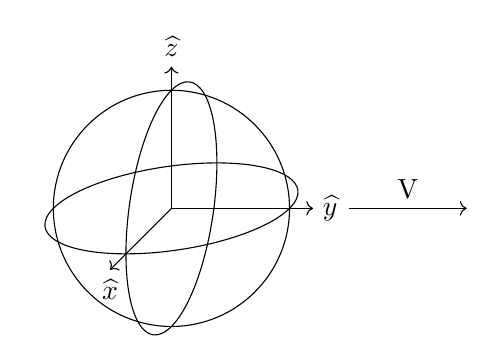
\begin{tikzpicture}[scale=1.5]
   \begin{scope}[canvas is zy plane at x=0]
     \draw (0,0) circle (1cm);
     %\draw[ultra thin] (-1,0) -- (1,0) (0,-1) -- (0,1);
     \draw[->] (0,0) -- (1.35,0) node[below ] {$\widehat{x}$};
   \end{scope}

   \begin{scope}[canvas is zx plane at y=0]
     \draw (0,0) circle (1cm);
     %\draw (-1,0) -- (1,0) (0,-1) -- (0,1);
     \draw[->] (0,0) -- (0,1.2) node[right] {$\widehat{y}$};
   \end{scope}

   \begin{scope}[canvas is xy plane at z=0]
     \draw (0,0) circle (1cm);
	%\draw (-1,0) -- (1,0) (0,-1) -- (0,1);
	\draw[->] (0,0) -- (0,1.2) node[above] {$\widehat{z}$};
   \end{scope}

 
    
   \draw[->] (1.5,0) -- node[above] {V} ++(1.0, 0) ;
 \end{tikzpicture}
 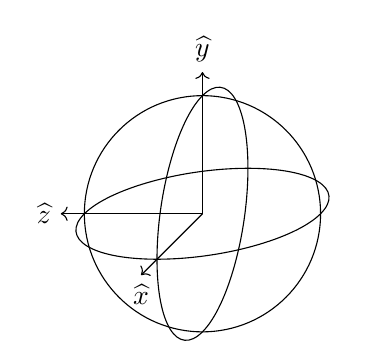
\begin{tikzpicture}[scale=1.5]
    \begin{scope}[canvas is zy plane at x=0]
     \draw (0,0) circle (1cm);
     %\draw[ultra thin] (-1,0) -- (1,0) (0,-1) -- (0,1);
     \draw[->] (0,0) -- (1.35,0) node[below ] {$\widehat{x}$};
   \end{scope}

   \begin{scope}[canvas is zx plane at y=0]
     \draw (0,0) circle (1cm);
     %\draw (-1,0) -- (1,0) (0,-1) -- (0,1);
     \draw[->] (0,0) -- (0,-1.2) node[left] {$\widehat{z}$};
   \end{scope}

   \begin{scope}[canvas is xy plane at z=0]
     \draw (0,0) circle (1cm);
	%\draw (-1,0) -- (1,0) (0,-1) -- (0,1);
	\draw[->] (0,0) -- (0,1.2) node[above] {$\widehat{y}$};
   \end{scope}
	 
 \end{tikzpicture}
 }
 \end{center}


\paragraph{Inverse V gate}\index{inverse V gate} Since the V-gate isn't Hermitian, the inverse gate, $V^\dagger$, is a distinct square root of $X$. 
\[
V^\dagger 
  & = X^{-\half}
\\ \notag
& = \half \begin{bmatrix*}[r] 1-i & 1+i \\ 1+i & 1-i \end{bmatrix*}
\\ \notag
& = H S^\dagger H
\\ \notag
& \simeq R_x(-\tfrac{\pi}{2})
\] 
\begin{center}
\adjustbox{scale=0.8}{\begin{quantikz}[thin lines, column sep=0.75em,row sep={2.5em,between origins}]
& \gate{V^\dagger} & \qw
\end{quantikz}
} or 
\adjustbox{scale=0.8}{\begin{quantikz}[thin lines, column sep=0.75em,row sep={2.5em,between origins}]
& \gate{X^{- \frac{1}{2}}} & \qw
\end{quantikz}
} 
\end{center}

\todo{Circuit}

A quarter turn clockwise about the $\widehat{x}$ axis.
\begin{center}
\adjustbox{scale=0.75}{
 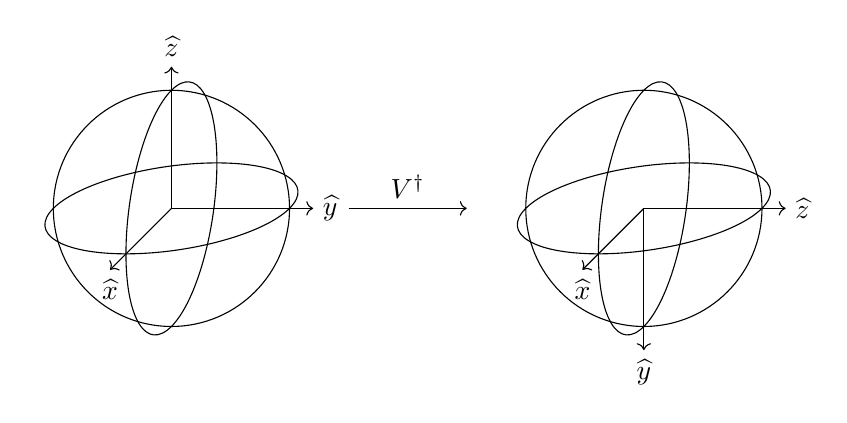
\begin{tikzpicture}[scale=1.5]
   \begin{scope}[canvas is zy plane at x=0]
     \draw (0,0) circle (1cm);
     %\draw[ultra thin] (-1,0) -- (1,0) (0,-1) -- (0,1);
     \draw[->] (0,0) -- (1.35,0) node[below ] {$\widehat{x}$};
   \end{scope}

   \begin{scope}[canvas is zx plane at y=0]
     \draw (0,0) circle (1cm);
     %\draw (-1,0) -- (1,0) (0,-1) -- (0,1);
     \draw[->] (0,0) -- (0,1.2) node[right] {$\widehat{y}$};
   \end{scope}

   \begin{scope}[canvas is xy plane at z=0]
     \draw (0,0) circle (1cm);
	%\draw (-1,0) -- (1,0) (0,-1) -- (0,1);
	\draw[->] (0,0) -- (0,1.2) node[above] {$\widehat{z}$};
   \end{scope}

 

   \draw[->] (1.5,0) -- node[above] {$V^\dagger$} ++(1.0, 0) ;

 \begin{scope}[xshift=4.0cm] 
    \begin{scope}[canvas is zy plane at x=0]
     \draw (0,0) circle (1cm);
     %\draw[ultra thin] (-1,0) -- (1,0) (0,-1) -- (0,1);
     \draw[->] (0,0) -- (1.35,0) node[below ] {$\widehat{x}$};
   \end{scope}

   \begin{scope}[canvas is zx plane at y=0]
     \draw (0,0) circle (1cm);
     %\draw (-1,0) -- (1,0) (0,-1) -- (0,1);
     \draw[->] (0,0) -- (0,1.2) node[right] {$\widehat{z}$};
   \end{scope}

   \begin{scope}[canvas is xy plane at z=0]
     \draw (0,0) circle (1cm);
	%\draw (-1,0) -- (1,0) (0,-1) -- (0,1);
	\draw[->] (0,0) -- (0,-1.2) node[below] {$\widehat{y}$};
   \end{scope}
	 \end{scope}
 \end{tikzpicture}
 }
 \end{center}



\paragraph{Pseudo-Hadamard gate}~\cite{Jones1998a, Dorai2000a}\index{pseudo-Hadamard gate}:
Inverse square root of the Y-gate.\index{square-root Y-gate}
% https://arxiv.org/pdf/quant-ph/9805070.pdf # Descriptions
% https://arxiv.org/pdf/quant-ph/0006103.pdf # uses
\[
h & = \tfrac{\sqrt{2}}{1+i} Y^{-\half}
\\ \notag
& = \tfrac{1}{\sqrt{2}}\begin{bmatrix*}[r]1 & 1 \\ -1 & 1 \end{bmatrix*}
\]
\begin{center}
\adjustbox{scale=0.9}{\begin{quantikz}[thin lines, column sep=0.75em, row sep={2.5em,between origins}]
  & \gate{\text{h}} & \qw
  \end{quantikz}} 
or \adjustbox{scale=0.8}{\begin{quantikz}[thin lines, column sep=0.75em,row sep={2.5em,between origins}]
& \gate{Y^{{-\frac{{1}}{{2}}}}} & \qw
\end{quantikz}
}
\end{center}
A quarter turn clockwise about the $\widehat{y}$ axis.
\begin{center}
\adjustbox{scale=0.75}{
 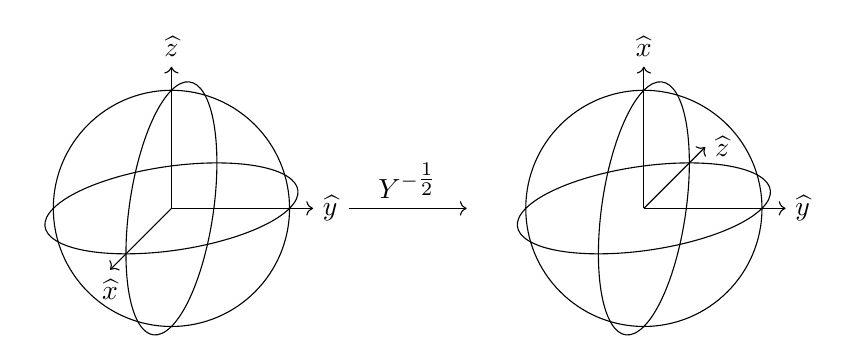
\begin{tikzpicture}[scale=1.5]
   \begin{scope}[canvas is zy plane at x=0]
     \draw (0,0) circle (1cm);
     %\draw[ultra thin] (-1,0) -- (1,0) (0,-1) -- (0,1);
     \draw[->] (0,0) -- (1.35,0) node[below ] {$\widehat{x}$};
   \end{scope}

   \begin{scope}[canvas is zx plane at y=0]
     \draw (0,0) circle (1cm);
     %\draw (-1,0) -- (1,0) (0,-1) -- (0,1);
     \draw[->] (0,0) -- (0,1.2) node[right] {$\widehat{y}$};
   \end{scope}

   \begin{scope}[canvas is xy plane at z=0]
     \draw (0,0) circle (1cm);
	%\draw (-1,0) -- (1,0) (0,-1) -- (0,1);
	\draw[->] (0,0) -- (0,1.2) node[above] {$\widehat{z}$};
   \end{scope}


   \draw[->] (1.5,0) -- node[above] {$Y^{-\half}$} ++(1.0, 0) ;

 \begin{scope}[xshift=4.0cm] 
    \begin{scope}[canvas is zy plane at x=0]
     \draw (0,0) circle (1cm);
     %\draw[ultra thin] (-1,0) -- (1,0) (0,-1) -- (0,1);
     \draw[->] (0,0) -- (-1.35,0) node[right ] {$\widehat{z}$};
   \end{scope}

   \begin{scope}[canvas is zx plane at y=0]
     \draw (0,0) circle (1cm);
     %\draw (-1,0) -- (1,0) (0,-1) -- (0,1);
     \draw[->] (0,0) -- (0,1.2) node[right] {$\widehat{y}$};
   \end{scope}

   \begin{scope}[canvas is xy plane at z=0]
     \draw (0,0) circle (1cm);
	%\draw (-1,0) -- (1,0) (0,-1) -- (0,1);
	\draw[->] (0,0) -- (0,1.2) node[above] {$\widehat{x}$};
   \end{scope}
	 \end{scope}
 \end{tikzpicture}
 }
 \end{center}

This square-root of the $Y$-gate is called the pseudo-Hadamard gate as it has the same effect on the computational basis as the Hadamard gate. % TODO: RefSee p???.
\[
h\ket{0} & = \ket{+} \notag \\ 
h\ket{1} & = \ket{-} \notag
\]


\paragraph{Inverse pseudo-Hadamard gate}\index{inverse pseudo-Hadamard gate}\index{square-root Y-gate} Principle square root of the Y-gate. Unlike the Hadamard gate, the pseudo-Hadamard gate is not Hermitian, and therefore not its own inverse. 
\[
h^\dagger &=\frac{1}{\sqrt{2}}\begin{bmatrix*}[r] 1 & -1 \\ 1 & 1 \end{bmatrix*}
\\
& = \tfrac{\sqrt{2}}{1+i} Y^{\half} \notag
\]
\begin{center}
\adjustbox{scale=0.9}{\begin{quantikz}[thin lines, column sep=0.75em, row sep={2.5em,between origins}]
& \gate{\text{h$^\dagger$}} & \qw
\end{quantikz}
} or \adjustbox{scale=0.8}{\begin{quantikz}[thin lines, column sep=0.75em,row sep={2.5em,between origins}]
& \gate{Y^{{\frac{{1}}{{2}}}}} & \qw
\end{quantikz}
}
\end{center}

A quarter turn anti-clockwise about the $\widehat{y}$ axis.
\begin{center}
\adjustbox{scale=0.75}{
 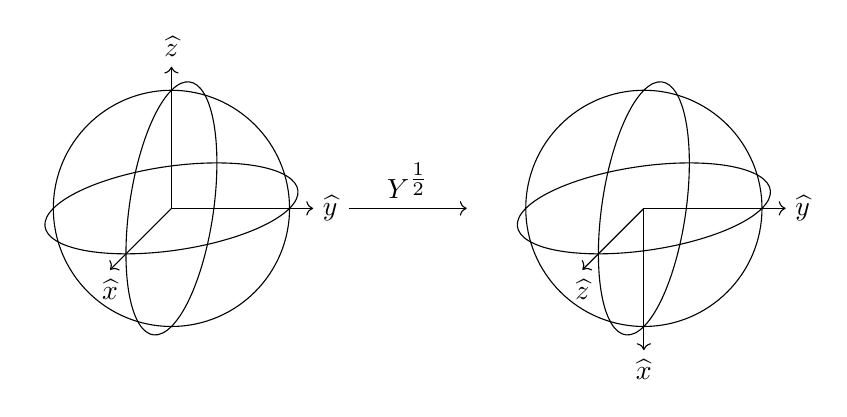
\begin{tikzpicture}[scale=1.5]
   \begin{scope}[canvas is zy plane at x=0]
     \draw (0,0) circle (1cm);
     %\draw[ultra thin] (-1,0) -- (1,0) (0,-1) -- (0,1);
     \draw[->] (0,0) -- (1.35,0) node[below ] {$\widehat{x}$};
   \end{scope}

   \begin{scope}[canvas is zx plane at y=0]
     \draw (0,0) circle (1cm);
     %\draw (-1,0) -- (1,0) (0,-1) -- (0,1);
     \draw[->] (0,0) -- (0,1.2) node[right] {$\widehat{y}$};
   \end{scope}

   \begin{scope}[canvas is xy plane at z=0]
     \draw (0,0) circle (1cm);
	%\draw (-1,0) -- (1,0) (0,-1) -- (0,1);
	\draw[->] (0,0) -- (0,1.2) node[above] {$\widehat{z}$};
   \end{scope}


   \draw[->] (1.5,0) -- node[above] {$Y^{\half}$} ++(1.0, 0) ;

 \begin{scope}[xshift=4.0cm] 
    \begin{scope}[canvas is zy plane at x=0]
     \draw (0,0) circle (1cm);
     %\draw[ultra thin] (-1,0) -- (1,0) (0,-1) -- (0,1);
     \draw[->] (0,0) -- (1.35,0) node[below ] {$\widehat{z}$};
   \end{scope}

   \begin{scope}[canvas is zx plane at y=0]
     \draw (0,0) circle (1cm);
     %\draw (-1,0) -- (1,0) (0,-1) -- (0,1);
     \draw[->] (0,0) -- (0,1.2) node[right] {$\widehat{y}$};
   \end{scope}

   \begin{scope}[canvas is xy plane at z=0]
     \draw (0,0) circle (1cm);
	%\draw (-1,0) -- (1,0) (0,-1) -- (0,1);
	\draw[->] (0,0) -- (0,-1.2) node[below] {$\widehat{x}$};
   \end{scope}
	 \end{scope}
 \end{tikzpicture}
 }
 \end{center}



\paragraph{S gate} (Phase, P, ``ess'')
\index{S gate}%
\index{Phase gate|see {S gate}}%
\index{P gate|see {S gate}}%
 Square root of the $Z$-gate, $SS=Z$.
%\index{\adjustbox{scale=0.8}{\begin{quantikz}[thin lines, column sep=0.75em,row sep={2.5em,between origins}]
& \gate{S} & \qw
\end{quantikz}
}@S|see{S gate}}
\[ 
S & = Z^{\half} \\
&= \begin{bmatrix}1 & 0 \\ 0 & i \end{bmatrix}
\notag
\\ \notag
& \simeq R_z(+\tfrac{\pi}{2})
\]
\begin{center}
\adjustbox{scale=0.8}{\begin{quantikz}[thin lines, column sep=0.75em,row sep={2.5em,between origins}]
& \gate{S} & \qw
\end{quantikz}
}
\end{center}

Historically called the phase gate (and denoted by $P$), since it shifts the phase of the one state relative to the zero state. This is a bit confusing because we have to make the distinction between the phase gate and applying a global phase. Often referred to as simple the S (``ess'') gate in contemporary discourse. 


\begin{center}
\adjustbox{scale=0.75}{
 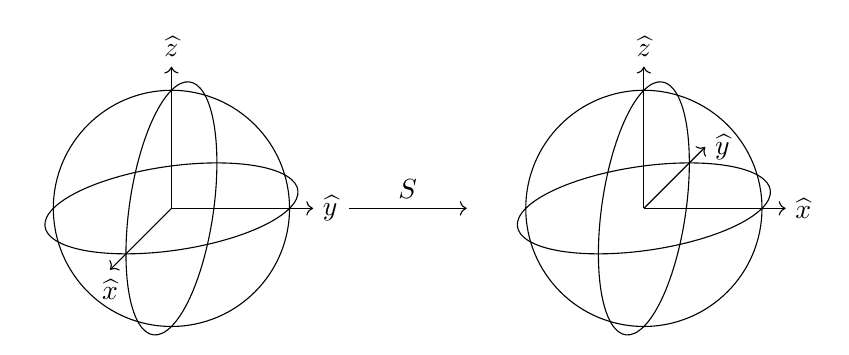
\begin{tikzpicture}[scale=1.5]
   \begin{scope}[canvas is zy plane at x=0]
     \draw (0,0) circle (1cm);
     %\draw[ultra thin] (-1,0) -- (1,0) (0,-1) -- (0,1);
     \draw[->] (0,0) -- (1.35,0) node[below ] {$\widehat{x}$};
   \end{scope}

   \begin{scope}[canvas is zx plane at y=0]
     \draw (0,0) circle (1cm);
     %\draw (-1,0) -- (1,0) (0,-1) -- (0,1);
     \draw[->] (0,0) -- (0,1.2) node[right] {$\widehat{y}$};
   \end{scope}

   \begin{scope}[canvas is xy plane at z=0]
     \draw (0,0) circle (1cm);
	%\draw (-1,0) -- (1,0) (0,-1) -- (0,1);
	\draw[->] (0,0) -- (0,1.2) node[above] {$\widehat{z}$};
   \end{scope}

 

   \draw[->] (1.5,0) -- node[above] {$S$} ++(1.0, 0) ;

 \begin{scope}[xshift=4.0cm] 
   \begin{scope}[canvas is zy plane at x=0]
     \draw (0,0) circle (1cm);
     %\draw[ultra thin] (-1,0) -- (1,0) (0,-1) -- (0,1);
     \draw[->] (0,0) -- (-1.35,0) node[right ] {$\widehat{y}$};
   \end{scope}

   \begin{scope}[canvas is zx plane at y=0]
     \draw (0,0) circle (1cm);
     %\draw (-1,0) -- (1,0) (0,-1) -- (0,1);
     \draw[->] (0,0) -- (0,1.2) node[right] {$\widehat{x}$};
   \end{scope}

   \begin{scope}[canvas is xy plane at z=0]
     \draw (0,0) circle (1cm);
	%\draw (-1,0) -- (1,0) (0,-1) -- (0,1);
	\draw[->] (0,0) -- (0,1.2) node[above] {$\widehat{z}$};
   \end{scope}
	 \end{scope}
 \end{tikzpicture}
 }
 \end{center}



\paragraph{Inverse S gate}\index{inverse S gate} Hermitian conjugate of the $S$ gate, and an alternative square-root of $Z$, $S^\dagger S^\dagger = Z$.
\[
S^\dagger 
& = Z^{-\half}
\\
&= \begin{bmatrix} 1 & 0 \\ 0 & -i \end{bmatrix}
\notag 
\\ \notag
& \simeq R_z(-\tfrac{\pi}{2})
\]
\begin{center}
\adjustbox{scale=0.8}{\begin{quantikz}[thin lines, column sep=0.75em,row sep={2.5em,between origins}]
& \gate{S^\dagger} & \qw
\end{quantikz}
}
\end{center}
\todo{alt Circuit}

A quarter turn clockwise about the $\widehat{z}$ axis.
\begin{center}
\adjustbox{scale=0.75}{
 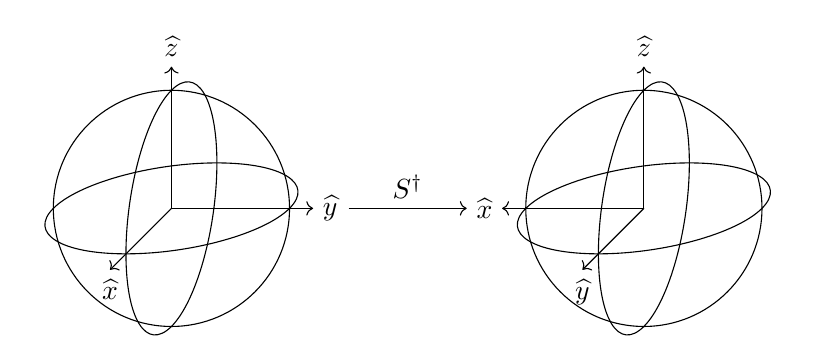
\begin{tikzpicture}[scale=1.5]
   \begin{scope}[canvas is zy plane at x=0]
     \draw (0,0) circle (1cm);
     %\draw[ultra thin] (-1,0) -- (1,0) (0,-1) -- (0,1);
     \draw[->] (0,0) -- (1.35,0) node[below ] {$\widehat{x}$};
   \end{scope}

   \begin{scope}[canvas is zx plane at y=0]
     \draw (0,0) circle (1cm);
     %\draw (-1,0) -- (1,0) (0,-1) -- (0,1);
     \draw[->] (0,0) -- (0,1.2) node[right] {$\widehat{y}$};
   \end{scope}

   \begin{scope}[canvas is xy plane at z=0]
     \draw (0,0) circle (1cm);
	%\draw (-1,0) -- (1,0) (0,-1) -- (0,1);
	\draw[->] (0,0) -- (0,1.2) node[above] {$\widehat{z}$};
   \end{scope}

 

   \draw[->] (1.5,0) -- node[above] {$S^\dagger$} ++(1.0, 0) ;

 \begin{scope}[xshift=4.0cm] 
   \begin{scope}[canvas is zy plane at x=0]
     \draw (0,0) circle (1cm);
     %\draw[ultra thin] (-1,0) -- (1,0) (0,-1) -- (0,1);
     \draw[->] (0,0) -- (1.35,0) node[below ] {$\widehat{y}$};
   \end{scope}

   \begin{scope}[canvas is zx plane at y=0]
     \draw (0,0) circle (1cm);
     %\draw (-1,0) -- (1,0) (0,-1) -- (0,1);
     \draw[->] (0,0) -- (0,-1.2) node[left] {$\widehat{x}$};
   \end{scope}

   \begin{scope}[canvas is xy plane at z=0]
     \draw (0,0) circle (1cm);
	%\draw (-1,0) -- (1,0) (0,-1) -- (0,1);
	\draw[->] (0,0) -- (0,1.2) node[above] {$\widehat{z}$};
   \end{scope}

	 \end{scope}
 \end{tikzpicture}
 }
 \end{center}
Can be generated from the $S$ gate, $SSS= S^\dagger$.




\subsection{Hadamard gates}
\label{sec:Hadamard}

\paragraph{Hadamard gate}\index{Hadamard gate}
\index{H gate@\Gate{H} gate|see {Hadamard gate}}
\index{H|see {Hamiltonian}}
The Hadamard gate is one of the most interesting and useful of the common gates. Its effect is a $\pi$ rotation (half turn) in the Bloch sphere about the axis
$\tfrac{1}{\sqrt{2}}(\widehat{x}+\widehat{z})$. % FIXME: \hat not working!?
In a sense the Hadamard gate is half way between the Z and X gates (Fig.~\ref{Fig:GateCoords}).
%
\[
H & = \tfrac{1}{\sqrt{2}}\begin{bmatrix*}[r]1 & 1 \\ 1 & -1 \end{bmatrix*} \\
	& \simeq R_{\vec{n}}(\pi), \quad \vec{n} = \tfrac{1}{\sqrt{2}}(1, 0, 1) \notag
\]

\begin{center}
\adjustbox{scale=0.8}{\begin{quantikz}[thin lines, column sep=0.75em,row sep={2.5em,between origins}]
& \gate{H} & \qw
\end{quantikz}
}
\end{center}



In terms of the Bloch sphere, the Hadamard gate interchanges the $\widehat{x}$ and $\widehat{z}$ axes, and inverts the $\widehat{y}$ axis.
\makeatletter
\tikzoption{canvas is plane}[]{\@setOxy#1}
\def\@setOxy O(#1,#2,#3)x(#4,#5,#6)y(#7,#8,#9)%
  {\def\tikz@plane@origin{\pgfpointxyz{#1}{#2}{#3}}%
   \def\tikz@plane@x{\pgfpointxyz{#4}{#5}{#6}}%
   \def\tikz@plane@y{\pgfpointxyz{#7}{#8}{#9}}%
   \tikz@canvas@is@plane
  }
\makeatother  

\begin{center}
\adjustbox{scale=0.75}{
 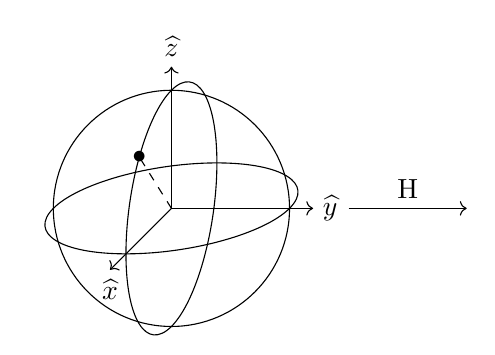
\begin{tikzpicture}[scale=1.5]
   \begin{scope}[canvas is zy plane at x=0]
     \draw (0,0) circle (1cm);
     %\draw[ultra thin] (-1,0) -- (1,0) (0,-1) -- (0,1);
     \draw[->] (0,0) -- (1.35,0) node[below ] {$\widehat{x}$};
     \draw[dashed] (0,0) -- (0.707,0.707) node {$\bullet$} ;
   \end{scope}

   \begin{scope}[canvas is zx plane at y=0]
     \draw (0,0) circle (1cm);
     %\draw (-1,0) -- (1,0) (0,-1) -- (0,1);
     \draw[->] (0,0) -- (0,1.2) node[right] {$\widehat{y}$};
   \end{scope}

   \begin{scope}[canvas is xy plane at z=0]
     \draw (0,0) circle (1cm);
	%\draw (-1,0) -- (1,0) (0,-1) -- (0,1);
	\draw[->] (0,0) -- (0,1.2) node[above] {$\widehat{z}$};
   \end{scope}

   \begin{scope}[canvas is plane={O(0,0.707,0.707)x(1,0,0)y(0,1,-1)}]
   	\centerarc[blue,->](0,0)(105:285:0.25)
   \end{scope}  
    
   \draw[->] (1.5,0) -- node[above] {H} ++(1.0, 0) ;
 \end{tikzpicture}
 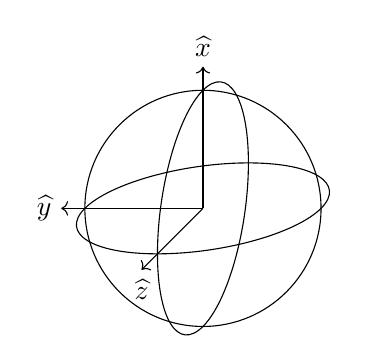
\begin{tikzpicture}[scale=1.5]
   \begin{scope}[canvas is zy plane at x=0]
     \draw (0,0) circle (1cm);
     %\draw[ultra thin] (-1,0) -- (1,0) (0,-1) -- (0,1);
     \draw[->] (0,0) -- (1.35,0) node[below ] {$\widehat{z}$};
   \end{scope}

   \begin{scope}[canvas is zx plane at y=0]
     \draw (0,0) circle (1cm);
     %\draw (-1,0) -- (1,0) (0,-1) -- (0,1);
     \draw[->] (0,0) -- (0,-1.2) node[left] {$\widehat{y}$};
   \end{scope}

   \begin{scope}[canvas is xy plane at z=0]
     \draw (0,0) circle (1cm);
	%\draw (-1,0) -- (1,0) (0,-1) -- (0,1);
	\draw[->] (0,0) -- (0,1.2) node[above] {$\widehat{x}$};
   \end{scope}

	 
 \end{tikzpicture}
 }
 \end{center}
 
A Hadamard similarity transform interchanges $X$ and $Z$ gates,
\[
HXH = Z, \qquad HYH &= -Y, \qquad HZH = X \notag 
\\
%\]
%\[
H R_x(\theta) H = R_z(\theta) , \qquad H R_y(\theta) H &= R_y(-\theta) , \qquad H R_z(\theta) H = R_x(\theta) 
\notag
\]

\todo{Rotation gate effect follows form Taylor expansion}


One reason that the Hadamard gate is so useful is that it acts on the computation basis states to create superpositions of zero and one states. These states are common enough that they have their own notation, $\ket{+}$ and \ket{-}.
\[
H\ket{0} & = \tfrac{1}{\sqrt{2}}(\ket{0}+\ket{1}) = \ket{+}
\notag
\\
H\ket{1} & = \tfrac{1}{\sqrt{2}}(\ket{0}-\ket{1}) = \ket{-} 
\notag
\]
The square of the Hadamard gate is the identity $HH=I$. This is easy to show with some simple algebra, or by considering that the Hadamard is a 180 degree rotation in the Bloch sphere, or by noting that the Hadamard matrix is both Hermitian and unitary, so the Hadamard must be its own inverse. As a consequence, the Hadamard converts the \ket{+}, \ket{-} Hadamard basis back to the \ket{0}, \ket{1} computational basis.
\index{computational basis} \index{Hadamard basis} \index{$\ket{+}$}\index{$\ket{-}$}
\[
H\ket{+} & = \ket{0} \notag \\ 
H\ket{-} & = \ket{1} \notag
\notag
\]

The Hadamard gate is named for the \define{Hadamard transform} (Or \define{Walsh-Hadamard transform}), which in the context of quantum computing is the simultaneous application of Hadamard gates to multiple-qubits. We will return this transform presently \secref{???}. The Hadamard gate is also the 1-qubit quantum Fourier transform \secref{???}\index{Hadamard transform}\index{Walsh-Hadamard transform|see {Hadamard transform}} \index{quantum Fourier transform! 1-qubit}
% TODO: Is this correct? Of is general Walsh-Hadamard QFT?

It is also worth noting a couple of useful decompositions (up to phase).
\begin{center}
\adjustbox{scale=0.8}{\begin{quantikz}[thin lines, column sep=0.75em,row sep={2.5em,between origins}]
& \gate{H} & \qw
\end{quantikz}
} $\simeq$
\adjustbox{scale=0.8}{\begin{quantikz}[thin lines, column sep=0.75em,row sep={2.5em,between origins}]
& \gate{Z} & \gate{Y^{\frac{1}{2}}} & \qw
\end{quantikz}
}
\end{center}


\begin{center}
\adjustbox{scale=0.75}{
 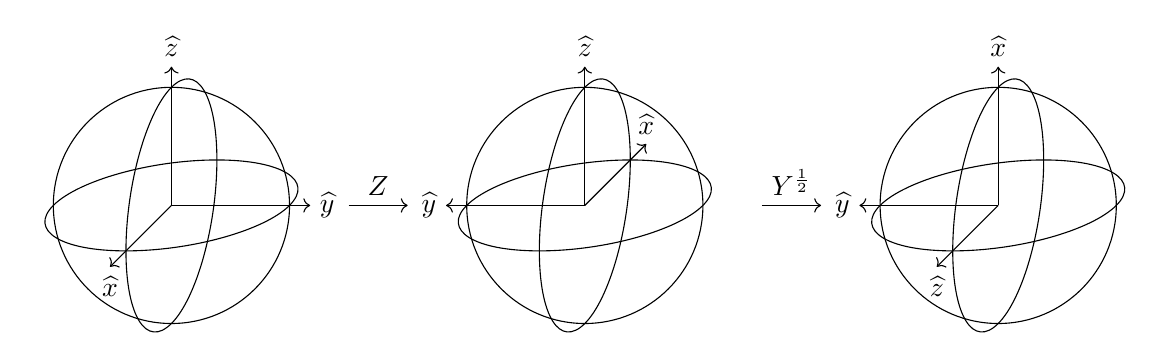
\begin{tikzpicture}[scale=1.5]
   \begin{scope}[canvas is zy plane at x=0]
     \draw (0,0) circle (1cm);
     %\draw[ultra thin] (-1,0) -- (1,0) (0,-1) -- (0,1);
     \draw[->] (0,0) -- (1.35,0) node[below] {$\widehat{x}$};
%     \draw[dashed] (0,0) -- (1.,1.) ;
   \end{scope}

   \begin{scope}[canvas is zx plane at y=0]
     \draw (0,0) circle (1cm);
     %\draw (-1,0) -- (1,0) (0,-1) -- (0,1);
     \draw[->] (0,0) -- (0,1.175) node[right] {$\widehat{y}$};
   \end{scope}

   \begin{scope}[canvas is xy plane at z=0]
     \draw (0,0) circle (1cm);
	%\draw (-1,0) -- (1,0) (0,-1) -- (0,1);
	\draw[->] (0,0) -- (0,1.175) node[above] {$\widehat{z}$};
   \end{scope}

%   \begin{scope}[canvas is zx plane at y=1.0]	
%   	\centerarc[blue,->](0,0)(270:90:0.25)
%   \end{scope}
    
   \draw[->] (1.5,0) -- node[above] {$Z$} ++(0.5, 0) ;

	\begin{scope}[xshift=3.5cm]
   \begin{scope}[canvas is zy plane at x=0]
     \draw (0,0) circle (1cm);
     %\draw[ultra thin] (-1,0) -- (1,0) (0,-1) -- (0,1);
     \draw[->] (0,0) -- (-1.35,0) node[above] {$\widehat{x}$};
   \end{scope}

   \begin{scope}[canvas is zx plane at y=0]
     \draw (0,0) circle (1cm);
     %\draw (-1,0) -- (1,0) (0,-1) -- (0,1);
     \draw[->] (0,0) -- (0,-1.175) node[left] {$\widehat{y}$};
   \end{scope}

   \begin{scope}[canvas is xy plane at z=0]
     \draw (0,0) circle (1cm);
	%\draw (-1,0) -- (1,0) (0,-1) -- (0,1);
	\draw[->] (0,0) -- (0,1.175) node[above] {$\widehat{z}$};
   \end{scope}
   \draw[->] (1.5,0) -- node[above] {$Y^{\frac{1}{2}}$} ++(0.5, 0) ;

	\end{scope}


	\begin{scope}[xshift=7.0cm]
   \begin{scope}[canvas is zy plane at x=0]
     \draw (0,0) circle (1cm);
     %\draw[ultra thin] (-1,0) -- (1,0) (0,-1) -- (0,1);
     \draw[->] (0,0) -- (1.35,0) node[below ] {$\widehat{z}$};
   \end{scope}

   \begin{scope}[canvas is zx plane at y=0]
     \draw (0,0) circle (1cm);
     %\draw (-1,0) -- (1,0) (0,-1) -- (0,1);
     \draw[->] (0,0) -- (0,-1.175) node[left] {$\widehat{y}$};
   \end{scope}

   \begin{scope}[canvas is xy plane at z=0]
     \draw (0,0) circle (1cm);
	%\draw (-1,0) -- (1,0) (0,-1) -- (0,1);
	\draw[->] (0,0) -- (0,1.175) node[above] {$\widehat{x}$};
   \end{scope}

	\end{scope}
 \end{tikzpicture}
}
 \end{center}

\begin{center}
\adjustbox{scale=0.8}{\begin{quantikz}[thin lines, column sep=0.75em,row sep={2.5em,between origins}]
& \gate{H} & \qw
\end{quantikz}
} $\simeq$
\adjustbox{scale=0.8}{\begin{quantikz}[thin lines, column sep=0.75em,row sep={2.5em,between origins}]
& \gate{S} & \gate{V} & \gate{S} & \qw
\end{quantikz}
}
\end{center}


\begin{center}
\adjustbox{scale=0.55}{
 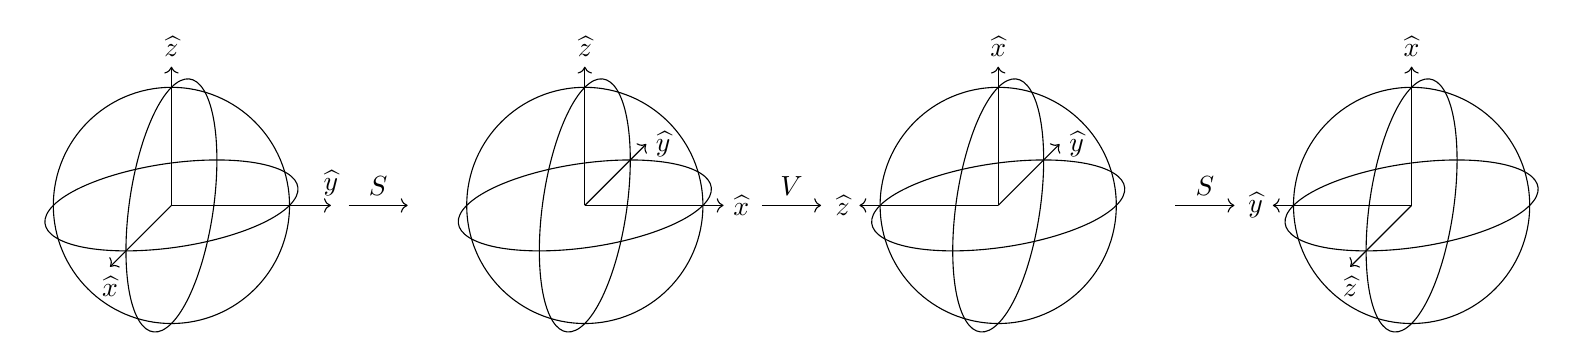
\begin{tikzpicture}[scale=1.5]
   \begin{scope}[canvas is zy plane at x=0]
     \draw (0,0) circle (1cm);
     %\draw[ultra thin] (-1,0) -- (1,0) (0,-1) -- (0,1);
     \draw[->] (0,0) -- (1.35,0) node[below] {$\widehat{x}$};
%     \draw[dashed] (0,0) -- (1.,1.) ;
   \end{scope}

   \begin{scope}[canvas is zx plane at y=0]
     \draw (0,0) circle (1cm);
     %\draw (-1,0) -- (1,0) (0,-1) -- (0,1);
     \draw[->] (0,0) -- (0,1.35) node[above] {$\widehat{y}$};
   \end{scope}

   \begin{scope}[canvas is xy plane at z=0]
     \draw (0,0) circle (1cm);
	%\draw (-1,0) -- (1,0) (0,-1) -- (0,1);
	\draw[->] (0,0) -- (0,1.175) node[above] {$\widehat{z}$};
   \end{scope}

%   \begin{scope}[canvas is zx plane at y=1.0]	
%   	\centerarc[blue,->](0,0)(270:90:0.25)
%   \end{scope}
    
   \draw[->] (1.5,0) -- node[above] {$S$} ++(0.5, 0) ;

	\begin{scope}[xshift=3.5cm]
    \begin{scope}[canvas is zy plane at x=0]
     \draw (0,0) circle (1cm);
     %\draw[ultra thin] (-1,0) -- (1,0) (0,-1) -- (0,1);
     \draw[->] (0,0) -- (-1.35,0) node[right] {$\widehat{y}$};
%     \draw[dashed] (0,0) -- (1.,1.) ;
   \end{scope}

   \begin{scope}[canvas is zx plane at y=0]
     \draw (0,0) circle (1cm);
     %\draw (-1,0) -- (1,0) (0,-1) -- (0,1);
     \draw[->] (0,0) -- (0,1.175) node[right] {$\widehat{x}$};
   \end{scope}

   \begin{scope}[canvas is xy plane at z=0]
     \draw (0,0) circle (1cm);
	%\draw (-1,0) -- (1,0) (0,-1) -- (0,1);
	\draw[->] (0,0) -- (0,1.175) node[above] {$\widehat{z}$};
   \end{scope}
      \draw[->] (1.5,0) -- node[above] {$V$} ++(0.5, 0) ;

	\end{scope}


	\begin{scope}[xshift=7.0cm]
   \begin{scope}[canvas is zy plane at x=0]
     \draw (0,0) circle (1cm);
     %\draw[ultra thin] (-1,0) -- (1,0) (0,-1) -- (0,1);
     \draw[->] (0,0) -- (-1.35,0) node[right] {$\widehat{y}$};
   \end{scope}

   \begin{scope}[canvas is zx plane at y=0]
     \draw (0,0) circle (1cm);
     %\draw (-1,0) -- (1,0) (0,-1) -- (0,1);
     \draw[->] (0,0) -- (0,-1.175) node[left] {$\widehat{z}$};
   \end{scope}

   \begin{scope}[canvas is xy plane at z=0]
     \draw (0,0) circle (1cm);
	%\draw (-1,0) -- (1,0) (0,-1) -- (0,1);
	\draw[->] (0,0) -- (0,1.175) node[above] {$\widehat{x}$};
   \end{scope}
   
   \draw[->] (1.5,0) -- node[above] {$S$} ++(0.5, 0) ;

	\end{scope}
	\begin{scope}[xshift=10.5cm]
   \begin{scope}[canvas is zy plane at x=0]
     \draw (0,0) circle (1cm);
     %\draw[ultra thin] (-1,0) -- (1,0) (0,-1) -- (0,1);
     \draw[->] (0,0) -- (1.35,0) node[below ] {$\widehat{z}$};
   \end{scope}

   \begin{scope}[canvas is zx plane at y=0]
     \draw (0,0) circle (1cm);
     %\draw (-1,0) -- (1,0) (0,-1) -- (0,1);
     \draw[->] (0,0) -- (0,-1.175) node[left] {$\widehat{y}$};
   \end{scope}

   \begin{scope}[canvas is xy plane at z=0]
     \draw (0,0) circle (1cm);
	%\draw (-1,0) -- (1,0) (0,-1) -- (0,1);
	\draw[->] (0,0) -- (0,1.175) node[above] {$\widehat{x}$};
   \end{scope}

	\end{scope}	
 \end{tikzpicture}
}
 \end{center}
 
Here, $V$ is the square-root of the $X$ gate, and $S$ is the square-root of Z, each of which is a quarter turn in the Bloch sphere.
 
 
% [TODO (elsewhere?): H is 1-qubit QFT. Multiqubit hadamard transform]   
% TODO
% 1-qubit Fourier transform
% Named for Hadamard transform (Walsh-Hadamard transform) 
% Explain +/- states, "polar basis" Hadamard basis? Also angled arrows?
% Create supposition of all computational basis states
% Hermitian, so own inverse
% When introduced into quantum computing?



\paragraph{Hadamard-like gates}
\index{Hadamard-like gates}
If we peruse the sphere of 1-qubit gates, Fig.~\ref{fig:GateCoords}, we can see that there are 6 different Hadamard-like gates that lie between the main \axis{x}, \axis{y}, and \axis{z} axes. (Recall that gates on opposite sides of the sphere's surface are the same up to phase.) Each of these gates can be obtained from straightforward transform so the Hadamard gate. For instance, $H_{YZ} = S H S^\dagger$ is the Hadamard-like gate between the $Z$ and $Y$ gates, which interchanges the \axis{y} and \axis{z} axies, and flips the \axis{x}-axis.


\begin{center}
\adjustbox{scale=0.75}{
 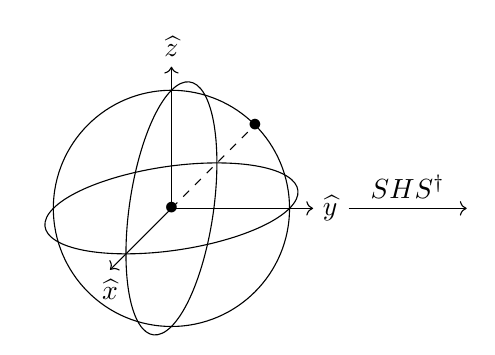
\begin{tikzpicture}[scale=1.5]
   \begin{scope}[canvas is zy plane at x=0]
     \draw (0,0) circle (1cm);
     %\draw[ultra thin] (-1,0) -- (1,0) (0,-1) -- (0,1);
     \draw[->] (0,0) -- (1.35,0) node[below ] {$\widehat{x}$};

   \end{scope}

   \begin{scope}[canvas is zx plane at y=0]
     \draw (0,0) circle (1cm);
     %\draw (-1,0) -- (1,0) (0,-1) -- (0,1);
     \draw[->] (0,0) -- (0,1.2) node[right] {$\widehat{y}$};
   \end{scope}

   \begin{scope}[canvas is xy plane at z=0]
     \draw (0,0) circle (1cm);
	%\draw (-1,0) -- (1,0) (0,-1) -- (0,1);
	\draw[->] (0,0) -- (0,1.2) node[above] {$\widehat{z}$};
	     \draw[dashed] (0,0) -- (0.707,0.707) node {$\bullet$};
   \end{scope}

%       \begin{scope}[canvas is plane={O(0.707,0.707,0)x(0,1,-1)y(1,0,0)}]
%       	\centerarc[blue,->](0,0)(290:105:0.25)
%       \end{scope}  

  \begin{scope}[canvas is plane={O(0.707,0.707,0)x(0,1,0)y(1,0,0)}]
   	\centerarc[thick, blue,->](0,0)(310:125:0.25)
	\draw (0,0) node {$\bullet$};
   \end{scope}  
             
    
   \draw[->] (1.5,0) -- node[above] {$S H S^\dagger$} ++(1.0, 0) ;
 \end{tikzpicture}
 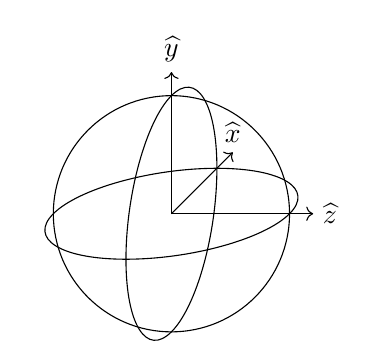
\begin{tikzpicture}[scale=1.5]
   \begin{scope}[canvas is zy plane at x=0]
     \draw (0,0) circle (1cm);
     %\draw[ultra thin] (-1,0) -- (1,0) (0,-1) -- (0,1);
     \draw[->] (0,0) -- (-1.35,0) node[above ] {$\widehat{x}$};
   \end{scope}

   \begin{scope}[canvas is zx plane at y=0]
     \draw (0,0) circle (1cm);
     %\draw (-1,0) -- (1,0) (0,-1) -- (0,1);
     \draw[->] (0,0) -- (0,1.2) node[right] {$\widehat{z}$};
   \end{scope}

   \begin{scope}[canvas is xy plane at z=0]
     \draw (0,0) circle (1cm);
	%\draw (-1,0) -- (1,0) (0,-1) -- (0,1);
	\draw[->] (0,0) -- (0,1.2) node[above] {$\widehat{y}$};
   \end{scope}

	 
 \end{tikzpicture}
 }
 \end{center}


\begin{figure}[tp]
%\begin{figure}[t]
\begin{center}
 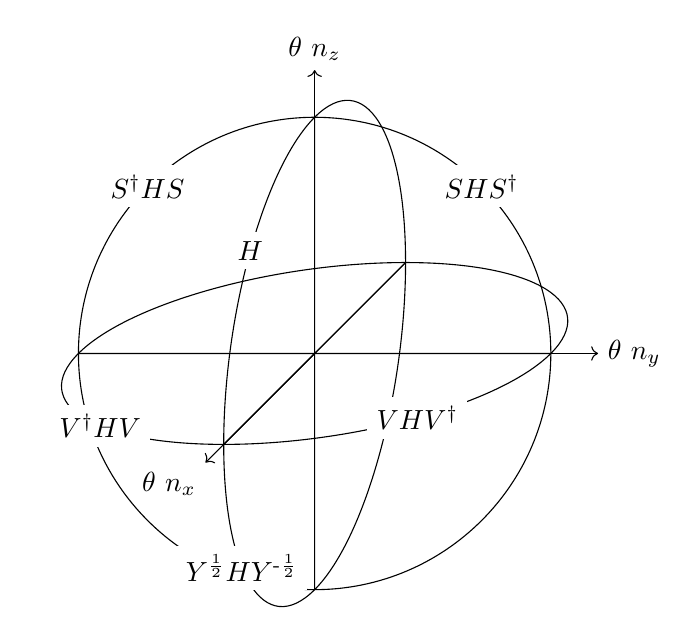
\begin{tikzpicture}[scale=3]
   \begin{scope}[canvas is zy plane at x=0]
     \draw (0,0) circle (1cm);
     \draw (-1,0) -- (1,0) (0,-1) -- (0,1);
     \draw[->] (0,0) -- (1.2,0) node[ below left] {$\theta\ n_x$};     
   \end{scope}

   \begin{scope}[canvas is zx plane at y=0]
     \draw (0,0) circle (1cm);
     \draw (-1,0) -- (1,0) (0,-1) -- (0,1);
     \draw[->] (0,0) -- (0,1.2) node[right ] {$\theta\ n_y$};     
   \end{scope}

   \begin{scope}[canvas is xy plane at z=0]
     \draw (0,0) circle (1cm);
     \draw (-1,0) -- (1,0) (0,-1) -- (0,1);
     \draw[->] (0,0) -- (0,1.2) node[above ] {$\theta\ n_z$};     
   \end{scope}

%	\node[fill=white] at (0,0,0) {$I$};
%
%	\node[fill=white] at (0,1,0) {$Z$};
%	\node[fill=white] at (0,0.5,0) {$S$};
%	\node[fill=white] at (0,0.25,0) {$T$};			
%	\node[fill=white] at (0,-0.5,0) {${S^\dagger}$};
%	\node[fill=white] at (0,-0.25,0) {$T^\dagger$};	
%	% \node[fill=white] at (0,-1,0) {Z};
%		
%	\node[fill=white] at (0,0,1) {$X$};
%	\node[fill=white] at (0,0,0.5) {$V$};
%	\node[fill=white] at (0,0,-0.5) {$V^\dagger$};	
%	% \node[fill=white] at (0,0,-1) {X};
%	
	\node[fill=white] at (0,{sqrt(1/2)},{sqrt(1/2)}) {$H$};
	\node[fill=white] at ({sqrt(1/2)},0, {sqrt(1/2)}) {$VHV^\dagger$};	
	\node[fill=white] at ({sqrt(1/2)},{sqrt(1/2)}, 0) {$SHS^\dagger$};	
	\node[fill=white] at (0,{-sqrt(1-0.64)}, {0.8}) {$Y^{\frac{1}{2}} H Y^{\text{-}\frac{1}{2}}$};
	\node[fill=white] at ({-sqrt(1-0.64)}, 0, {0.8}) {$V^\dagger H V$};	
	\node[fill=white] at ({-sqrt(1/2)},{sqrt(1/2)}, 0) {$S^\dagger H S$};
			
%%	\node[fill=white] at (0,0,1) {H};
%	
%	\node[fill=white] at (1,0,0) {$Y$};
%	\node[fill=white] at (0.5,0,0) {${h^\dagger}$};	
%	\node[fill=white] at (-0.5,0,0) {${h}$};	
	% \node[fill=white] at (-1,0,0) {$Y$};
 \end{tikzpicture}
 \end{center}
 \label{Fig:GateCoordsHadamard}
\caption{Coordinates of the 6-Hadamard like gates. \todo{CHECK!}}
\end{figure}
This particular Hadamard-like gate takes the computational Z-basis to the Y-basis.
\[
S H S^\dagger \ket{0} =  \tfrac{1}{\sqrt{2}}(\ket{0}+i\ket{1})  = \ket{+i} \notag \\
S H S^\dagger \ket{1} =  \tfrac{1}{\sqrt{2}}(\ket{0}-i\ket{1})  = \ket{-i} \notag
\]
% These Hadamard-like gates are all Clifford gates (\S \ref{ChClifford}), and 
The coordinates of all 6 Hadamard-like gates are shown in Fig.~\ref{Fig:GateCoordsHadamard}, and listed in Table~\ref{tab:Clifford1q} in the same block as the Hadamard gate. 

\todo{Maybe move to Clifford chapter}

%%
%%\paragraph{Hadamard power gate}
%%\todo{Define via Rn}
%%\todo{Not needed?}
%%
%%\[
%%H_H = \frac{\pi}{2} (\frac{1}{\sqrt{2}}(X + Z) - I)
%%\notag
%%\]
%%
%%\[
%% H^t = e^{i \pi t/2}
%%        \begin{bmatrix*}[r]
%%            \cos(\tfrac{t}{2}) + \tfrac{i}{\sqrt{2}}\sin(\tfrac{t}{2}) &
%%            \tfrac{i}{\sqrt{2}} \sin(\tfrac{t}{2}) \\
%%            \tfrac{i}{\sqrt{2}} \sin(\tfrac{t}{2}) &
%%            \cos(\tfrac{t}{2}) -\tfrac{i}{\sqrt{2}} \sin(\frac{t}{2})
%%        \end{bmatrix*}
%%\]
%%
%%
%%\begin{center}
%%\adjustbox{scale=0.75}{
%% \begin{tikzpicture}[scale=1.5]
%%   \begin{scope}[canvas is zy plane at x=0]
%%     \draw (0,0) circle (1cm);
%%     %\draw[ultra thin] (-1,0) -- (1,0) (0,-1) -- (0,1);
%%     \draw[->] (0,0) -- (1.35,0) node[below ] {$\widehat{x}$};
%%     \draw[dashed] (0,0) -- (0.707,0.707) node {$\bullet$} ;
%%   \end{scope}
%%
%%   \begin{scope}[canvas is zx plane at y=0]
%%     \draw (0,0) circle (1cm);
%%     %\draw (-1,0) -- (1,0) (0,-1) -- (0,1);
%%     \draw[->] (0,0) -- (0,1.2) node[right] {$\widehat{y}$};
%%   \end{scope}
%%
%%   \begin{scope}[canvas is xy plane at z=0]
%%     \draw (0,0) circle (1cm);
%%	%\draw (-1,0) -- (1,0) (0,-1) -- (0,1);
%%	\draw[->] (0,0) -- (0,1.2) node[above] {$\widehat{z}$};
%%   \end{scope}
%%
%%   \begin{scope}[canvas is plane={O(0,0.707,0.707)x(1,0,0)y(0,1,-1)}]
%%   	\centerarc[blue,->](0,0)(105:285:0.25)
%%   \end{scope}  
%%    
%%	 
%% \end{tikzpicture}
%% }
%% \end{center}
%%%

\subsection{Axis cycling gates}
Another interesting, but rarely discussed\endnote{Period 3 axis cycling gates are widely discussed abstractly in the context of Clifford gates \secref{sec:Clifford}. I've borrowed the explicit realization and nomenclature from 
Craig Gidney's \texttt{stim} python package, a simulator for quantum stabilizer circuits. \url{https://github.com/quantumlib/Stim} \cite{Gidney2021a}} class of gates are those that interchange three axes. These gates have periodicity 3 and represent 120 degree rotations of the Bloch sphere.
\index{axis cycling gates}\index{C gate|see{axis cycling gates}}

\paragraph{C gate}~\cite{Gidney2021a}
\[
C & = \tfrac{1}{2} \begin{bmatrix}+1-i & -1-i \\ +1-i &+1+i \end{bmatrix}
\\ \notag 
& = R_n(\tfrac{2}{3}\pi),\quad  n = (\tfrac{1}{\sqrt{3}},\tfrac{1}{\sqrt{3}},\tfrac{1}{\sqrt{3}})
\]
A right handed period 3 axis cycling gate, cycling the axes in the permutation $\axis{x}\rightarrow \axis{y} \rightarrow \axis{z} \rightarrow \axis{x}$
\[
C\ X^t\ C^\dagger &= Y^t \notag \\
C\ Y^t\ C^\dagger &= Z^t \notag \\
C\ Z^t\ C^\dagger &= X^t \notag
\]
Note that this is a third root of the identity, 
$C^3 = I$, and that the square gives the inverse gate $C^2 = C^\dagger$ which cycles in the opposite direction. 

There are 8 distinct axis cycling gates, which are all also Clifford gates, and listed in the last block of table~\ref{tab:Clifford1q}. Each such gate can be broken down into a combination of two quarter turns, e.g.~$C=SV$.


\begin{center}
\adjustbox{scale=0.75}{
 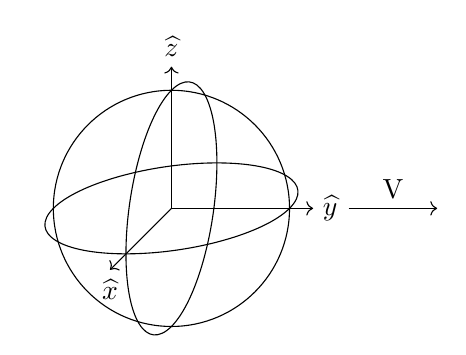
\begin{tikzpicture}[scale=1.5]
   \begin{scope}[canvas is zy plane at x=0]
     \draw (0,0) circle (1cm);
     %\draw[ultra thin] (-1,0) -- (1,0) (0,-1) -- (0,1);
     \draw[->] (0,0) -- (1.35,0) node[below ] {$\widehat{x}$};
   \end{scope}

   \begin{scope}[canvas is zx plane at y=0]
     \draw (0,0) circle (1cm);
     %\draw (-1,0) -- (1,0) (0,-1) -- (0,1);
     \draw[->] (0,0) -- (0,1.2) node[right] {$\widehat{y}$};
   \end{scope}

   \begin{scope}[canvas is xy plane at z=0]
     \draw (0,0) circle (1cm);
	%\draw (-1,0) -- (1,0) (0,-1) -- (0,1);
	\draw[->] (0,0) -- (0,1.2) node[above] {$\widehat{z}$};
   \end{scope}

 
    
   \draw[->] (1.5,0) -- node[above] {V} ++(0.75, 0) ;
 \end{tikzpicture}
 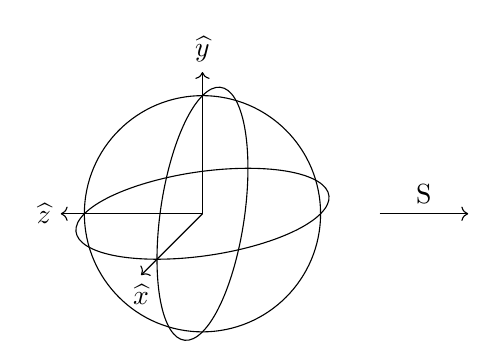
\begin{tikzpicture}[scale=1.5]
    \begin{scope}[canvas is zy plane at x=0]
     \draw (0,0) circle (1cm);
     %\draw[ultra thin] (-1,0) -- (1,0) (0,-1) -- (0,1);
     \draw[->] (0,0) -- (1.35,0) node[below ] {$\widehat{x}$};
   \end{scope}

   \begin{scope}[canvas is zx plane at y=0]
     \draw (0,0) circle (1cm);
     %\draw (-1,0) -- (1,0) (0,-1) -- (0,1);
     \draw[->] (0,0) -- (0,-1.2) node[left] {$\widehat{z}$};
   \end{scope}

   \begin{scope}[canvas is xy plane at z=0]
     \draw (0,0) circle (1cm);
	%\draw (-1,0) -- (1,0) (0,-1) -- (0,1);
	\draw[->] (0,0) -- (0,1.2) node[above] {$\widehat{y}$};
   \end{scope}
	   \draw[->] (1.5,0) -- node[above] {S} ++(0.75, 0) ;
 
 \end{tikzpicture}
 
 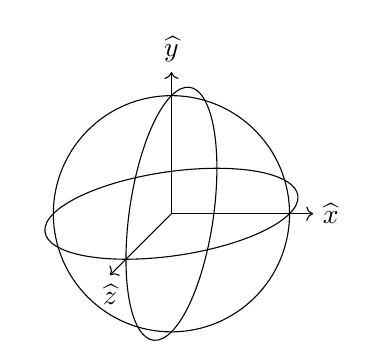
\begin{tikzpicture}[scale=1.5]
   \begin{scope}[canvas is zy plane at x=0]
     \draw (0,0) circle (1cm);
     %\draw[ultra thin] (-1,0) -- (1,0) (0,-1) -- (0,1);
     \draw[->] (0,0) -- (1.35,0) node[below ] {$\widehat{z}$};
   \end{scope}

   \begin{scope}[canvas is zx plane at y=0]
     \draw (0,0) circle (1cm);
     %\draw (-1,0) -- (1,0) (0,-1) -- (0,1);
     \draw[->] (0,0) -- (0,1.2) node[right] {$\widehat{x}$};
   \end{scope}

   \begin{scope}[canvas is xy plane at z=0]
     \draw (0,0) circle (1cm);
	%\draw (-1,0) -- (1,0) (0,-1) -- (0,1);
	\draw[->] (0,0) -- (0,1.2) node[above] {$\widehat{y}$};
   \end{scope}
 
 \end{tikzpicture}
 }
 \end{center}



\subsection{T gates}
All the of preceding discrete 1-qubit gates (Pauli gates, quarter turns, Hadamard and Hadamard-like gates, and axis cycling gates) are examples of a special class of gates called Clifford gates. Although important, the Clifford gates have the notable restricting that they aren't universal -- you can't build an arbitrary qubit rotation from Clifford gates alone. The is because the Clifford gates always map the \axis{x}, \axis{y} and \axis{z} axes back onto themselves. In order to be computational universal, it is necessary to have at least one non-Clifford gate in our gate set, and the most common choice for that non-Clifford gate is the $T$ gate, one eighth of a rotation anti-clockwise about the $z$ axis. A gate set consisting of all Cliffords (including multi-qubit Cliffords) and the T gate is often written as ``Clifford+T''.
\index{Clifford+T}\index{Clifford gates}

\todo{Wordsmith}


\paragraph{T gate} ("tee", $\pi/8$) Forth root of the $Z$ gate, $T^4=Z$.
\index{T gate}
\index{$\pi/8$ gate | see {T gate}}

\[
T & = Z^{\frac{1}{4}} \\
\notag
& = \begin{bmatrix}1 & 0 \\ 0 & e^{i \frac{\pi}{4}} \end{bmatrix}
\]
\begin{center}
\adjustbox{scale=0.8}{\begin{quantikz}[thin lines, column sep=0.75em,row sep={2.5em,between origins}]
& \gate{T} & \qw
\end{quantikz}
}
\end{center}

The T gate has sometimes been called the $\pi/8$ gate since we can extract a phase and write the T gate as
\[
T = e^{i\tfrac{\pi}{8}\pi} \begin{bmatrix} e^{-i\tfrac{\pi}{8}} & 0 \\ 0 & e^{+i\tfrac{\pi}{8}} 
\end{bmatrix}
\notag
\]

An eight turn anti-clockwise about the $\widehat{z}$ axis.
\begin{center}
\adjustbox{scale=0.75}{
 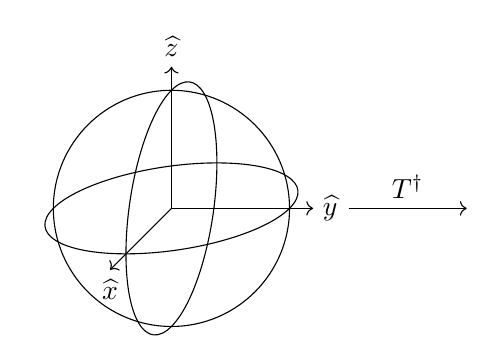
\begin{tikzpicture}[scale=1.5]
   \begin{scope}[canvas is zy plane at x=0]
     \draw (0,0) circle (1cm);
     %\draw[ultra thin] (-1,0) -- (1,0) (0,-1) -- (0,1);
     \draw[->] (0,0) -- (1.35,0) node[below ] {$\widehat{x}$};
   \end{scope}

   \begin{scope}[canvas is zx plane at y=0]
     \draw (0,0) circle (1cm);
     %\draw (-1,0) -- (1,0) (0,-1) -- (0,1);
     \draw[->] (0,0) -- (0,1.2) node[right] {$\widehat{y}$};
   \end{scope}

   \begin{scope}[canvas is xy plane at z=0]
     \draw (0,0) circle (1cm);
	%\draw (-1,0) -- (1,0) (0,-1) -- (0,1);
	\draw[->] (0,0) -- (0,1.2) node[above] {$\widehat{z}$};
   \end{scope}

 
    
   \draw[->] (1.5,0) -- node[above] {$T^\dagger$} ++(1.0, 0) ;
 \end{tikzpicture}
 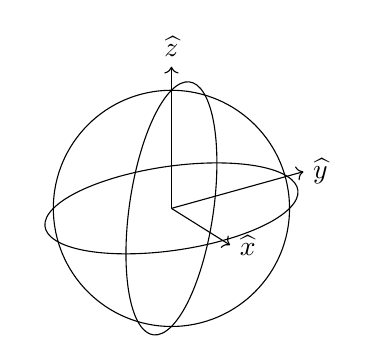
\begin{tikzpicture}[scale=1.5]
   \begin{scope}[canvas is zy plane at x=0]
     \draw (0,0) circle (1cm);

   \end{scope}

   \begin{scope}[canvas is zx plane at y=0]
     \draw (0,0) circle (1cm);
     %\draw (-1,0) -- (1,0) (0,-1) -- (0,1);
     \draw[->] (0,0) -- (0.807,0.807) node[right] {$\widehat{x}$};
     \draw[->] (0,0) -- (-0.807,0.807) node[right] {$\widehat{y}$};     
   \end{scope}

   \begin{scope}[canvas is xy plane at z=0]
     \draw (0,0) circle (1cm);
	%\draw (-1,0) -- (1,0) (0,-1) -- (0,1);
	\draw[->] (0,0) -- (0,1.2) node[above] {$\widehat{z}$};
   \end{scope}

	 
 \end{tikzpicture}
 }
 \end{center}


% TODO T-like gates, rotations on Y or X axis

\paragraph{Inverse T gate}Hermitian conjugate of the T gate.
\index{inverse T gate}
\[
T^\dagger & = Z^{-\frac{1}{4}} 
\\ 
\notag & = 
\begin{bmatrix} 
1 & 0 \\ 0 & e^{-i\tfrac{\pi}{4}} 
\end{bmatrix}
\\ \notag
& \simeq R_z(\tfrac{pi}{4})
\]
\begin{center}
\adjustbox{scale=0.8}{\begin{quantikz}[thin lines, column sep=0.75em,row sep={2.5em,between origins}]
& \gate{T^\dagger} & \qw
\end{quantikz}
}
\end{center}


An eighth turn clockwise about the \axis{z} axis.
\begin{center}
\adjustbox{scale=0.75}{
 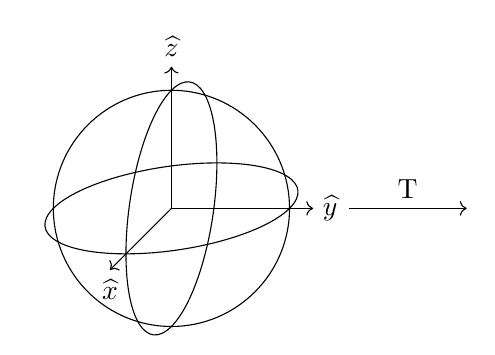
\begin{tikzpicture}[scale=1.5]
   \begin{scope}[canvas is zy plane at x=0]
     \draw (0,0) circle (1cm);
     %\draw[ultra thin] (-1,0) -- (1,0) (0,-1) -- (0,1);
     \draw[->] (0,0) -- (1.35,0) node[below ] {$\widehat{x}$};
   \end{scope}

   \begin{scope}[canvas is zx plane at y=0]
     \draw (0,0) circle (1cm);
     %\draw (-1,0) -- (1,0) (0,-1) -- (0,1);
     \draw[->] (0,0) -- (0,1.2) node[right] {$\widehat{y}$};
   \end{scope}

   \begin{scope}[canvas is xy plane at z=0]
     \draw (0,0) circle (1cm);
	%\draw (-1,0) -- (1,0) (0,-1) -- (0,1);
	\draw[->] (0,0) -- (0,1.2) node[above] {$\widehat{z}$};
   \end{scope}

 
    
   \draw[->] (1.5,0) -- node[above] {T} ++(1.0, 0) ;
 \end{tikzpicture}
 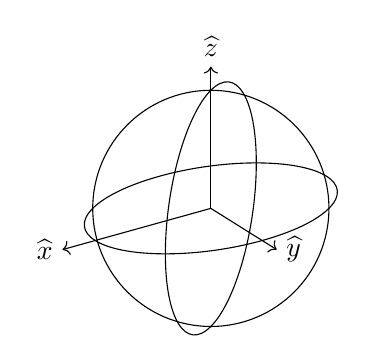
\begin{tikzpicture}[scale=1.5]
   \begin{scope}[canvas is zy plane at x=0]
     \draw (0,0) circle (1cm);

   \end{scope}

   \begin{scope}[canvas is zx plane at y=0]
     \draw (0,0) circle (1cm);
     %\draw (-1,0) -- (1,0) (0,-1) -- (0,1);
     \draw[->] (0,0) -- (0.907,-0.907) node[left] {$\widehat{x}$};
     \draw[->] (0,0) -- (0.907,0.907) node[right] {$\widehat{y}$};     
   \end{scope}

   \begin{scope}[canvas is xy plane at z=0]
     \draw (0,0) circle (1cm);
	%\draw (-1,0) -- (1,0) (0,-1) -- (0,1);
	\draw[->] (0,0) -- (0,1.2) node[above] {$\widehat{z}$};
   \end{scope}	 
 \end{tikzpicture}
 }
 \end{center}





\subsection{Global phase}

\paragraph{Global phase gate} (phase-shift)~\cite{Barenco1995b,???,???}
\index{phase}
\index{global phase gate}
\index{phase shift gate}
\[
\label{Ph}
\Gate{Ph}(\alpha) &= 􏰔 e^{i\alpha} I  \\
& = \begin{bmatrix} e^{i\alpha} & 0 \\ 0 & e^{i\alpha} \end{bmatrix}
\notag
\]
\begin{center}
\adjustbox{scale=0.8}{\begin{quantikz}[thin lines, column sep=0.75em,row sep={2.5em,between origins}]
& \gate{\text{Ph}(\alpha)} & \qw
\end{quantikz}
}
\end{center}
To shift the global phase we multiply the quantum state by a scalar, so it is not necessary to assign a phase shift to any particular qubit. But on those occasions where we want to keep explicit track of the phase in a circuit, it is useful to assign a global phase shift to a particular qubit and temporal location, e.g.\
\begin{center}
\adjustbox{scale=0.8}{\begin{quantikz}[thin lines, column sep=0.75em,row sep={2.5em,between origins}]
& \gate{R_x(\theta)} & \qw
\end{quantikz}
}
$=$
\adjustbox{scale=0.8}{\begin{quantikz}[thin lines, column sep=0.75em,row sep={2.5em,between origins}]
& \gate{\text{Ph}(-\frac{\theta}{2})} & \gate{X^{\frac{\theta}{\pi}}} & \qw
\end{quantikz}
}
\end{center}

This gate was originally called the phase-shift gate~\cite{Barenco1995b}, but unfortunately the 1-qubit gate that shifts the phase of the 1 state relative the the zero state is also called the phase-shift gate~\eqref{phaseshift},
which is potentially confusing. 


\paragraph{Omega gate}~\cite{???,???}
\index{omega gate}
\[
\label{omega}
\omega^k &= \text{Ph}(\tfrac{\pi}{4}k) 
\\
& = \begin{bmatrix} e^{i\frac{\pi}{4}k} & 0 \\ 0 & e^{i\frac{\pi}{4}k} \end{bmatrix}
\notag
\]
An alternative parameterization of a global phase shift. Note that this gate is an eight root of the identity,  $\omega^8=I$. This gate, with integer powers, crops up when constructing the 1-qubit Clifford gates from Hadamard and S gates, since $SHSHSH=\omega$ (see p.~\pageref{cliffordomega}).  
\index{global phase gate}


% [TODO: Remove figures to separate files]
% [TODO: Am I using the terms 'phase' and 'phase factor' consistantly]


% TODO: Talk about this when do 1-qubit deke
%    \paragraph{QASM U3 gate}
%    ...



% !TEX encoding = UTF-8 Unicode 
% !TEX root = on_gates.tex


\clearpage
\section{Decomposition of 1-qubit gates}
A general 1-qubit gate corresponds to some 2 by 2 unitary matrix,
\[
U = 
e^{i\alpha}\begin{bsmallmatrix}
a & -b^* \\
b & a^*
\end{bsmallmatrix}\]
where $a$ and $b$ are complex with $|a|^2 + |b|^2 = 1$, and  $\alpha$ is real.
Given such a generic unitary, we would like to represent this gate using standard parameterized gates.   

The first step to deke\footnote{
{\sl deke} {\sl |dek|} verb --- To decompile, deconstruct, or decompose.
\\ 1995  Neal Stephenson {\sl The Diamond Age} ``We gotta deke all this stuff now'' Easy come, easy go.
\index{deke}}\index{deke} a gate is to extract the phase factor $\alpha$,
\[
V = e^{-i\alpha} U
\]
so that $V$ is a special unitary matrix with $\det V=1$. In general, if we multiply a special unitary matrix by a complex phase $c$ then $\det cU=c^k$ where $k$ is the rank of the matrix, i.e. $k=2^n$ for $n$ qubits. This follows since the determinate is the product of the eigenvalues, and multiplying a matrix by a constant multiplies each eigenvalue by that constant.
Thus the determinate of $U$ is $\det U=e^{i 2 \alpha }$, and we can extract the phase factor $\alpha$ with some trigonometry.
\[
\alpha = \half \operatorname{arctan2}\bigl(\Im(\det U), \Re(\det U)\bigr)
\label{phase_extraction}
\]
% TODO: CHECK

The two-argument arctangent function $\operatorname{arctan2}(y,x)$ returns the angle~$\theta$ between x-axis and the ray from the origin to $(x, y)$. In contrast the single argument arctangent function $\arctan(y/x)$ only gives the correct answer for $x>0$ since it can't distinguish between $(x,y)$ and $(-x, -y)$.\index{arctan2}
\begin{center}
\begin{tikzpicture}[scale=0.75]
\draw[->] (-3,0) -- (3, 0);
\draw[->] (0,-3) -- (0, 3);
\draw[-o, dashed] (0,0) --(2.5, 2) node[right] {$(x,y)$} node [midway, above, sloped] (r) {$r$};
\draw[->] (0:2) arc[radius=2, start angle=0, end angle=35] node [midway, right] {$\theta = \operatorname{arctan2}(y,x)$};
\end{tikzpicture}
\end{center}
For a complex number $x+iy = r e^{i\theta}$, the modulus (or magnitude) $r=\sqrt{x^2+y^2}$ and the phase (or argument) is $\theta = \operatorname{arctan2}(y,x)$. 

\subsection{Z-Y-Z decomposition}\index{ZYZ decomposition}
\label{sec:ZYZdeke}
\index{Pauli-rotation decomposition}
\todo{Naming. Pauli deke? Euler? Z-Y-Z or Z-Y?}
Any 1-qubit gate can be decomposed as a sequence of Z, Y, and Z rotations, and a phase~\cite{Barenco1995b}\footnote{The Z-Y decomposition is of ancient origin, long know in the theory of light polarization~\cite{Sousa2006a}}.
\[
U =  e^{i\alpha}\ R_z(\theta_2)\ R_y(\theta_1)\ R_z(\theta_0)
\]
Or in circuit notation.
\begin{center}
\adjustbox{scale=0.75}{\begin{quantikz}[thin lines, column sep=0.75em,row sep={2.5em,between origins}]
& \gate{U} & \qw 
\end{quantikz}}
$=$
\adjustbox{scale=0.8}{\begin{quantikz}[thin lines, column sep=0.75em,row sep={2.5em,between origins}]
& \gate{R_z(\theta_{0})} & \gate{R_y(\theta_{1})} & \gate{R_z(\theta_{2})} & \gate{\text{Ph}(\alpha)} & \qw
\end{quantikz}
}
\end{center}
Note that we have numbered the three angles in chronological order, and recall that time runs right-to-left in operator notation, but left-to-right in circuit notation. 

%%For example, the $R_x$ gate can be generated by an $R_y$ gate sandwiched between quarter turns about the z-axis.
%%\[
%%\Gate{R_x}(\theta) =  \ R_z(-\tfrac{\pi}{2})\ R_y(\theta)\ R_z(+\tfrac{\pi}{2})
%%\]
If multiply out the circuit, then we get the following universal 1-qubit gate.
\[
U = 
e^{i\alpha} \begin{bmatrix}
+e^{-i\half\theta_2  -i\half\theta_0} \cos(\half\theta_1)
& -e^{-i\half\theta_2 + i\half\theta_0} \sin(\half\theta_1)
\\
+e^{+i\half\theta_2 - i\half\theta_0} \sin(\half\theta_1)
& +e^{+i\half\theta_2 +i\half\theta_0} \cos(\half\theta_1)
\end{bmatrix}
\]
The first step in the decomposition is to extract the phase using Eq.~\eqref{phase_extraction}, leaving a special unitary matrix $V = e^{-i\alpha} U$.
%
The value of $\theta_1$ can be calculated from the absolute value of either the diagonal or off-diagonal elements, provided those entries aren't close to zero.
For instance, the Z-gate has zero off-diagonal entries, whereas the X-gate has zeros on the diagonal. But the diagonal and off-diagonal entries can't approach zero at the same time.  So to calculate $\theta_1$ with greatest numerical accuracy, we use whichever element has the largest absolute value.
\[
\theta_1 = 
  \begin{cases}
		2 \arccos(|V_{00}|), & |V_{00}| \geq |V_{01}|\\	
		2 \arcsin(|V_{01}|), & |V_{00}| < |V_{01}|		
	\end{cases} 
\]

Having extracted $\theta_1$, we can now calculate the sum $\theta_0+\theta_1$ from $V_{11}$ using the $\operatorname{arctan2}$ function.\index{arctan2}
\[
 \theta_0 + \theta_2 =  
  2\ \operatorname{arctan2}\Left(\Im(\frac{V_{11}}{\cos(\half\theta_1)}),\ \Re(\frac{V_{11}}{\cos(\half\theta_1)})\Right)
\ .
\label{theta_sum}
\]
except if $\cos(\half\theta_1)=0$ then $\theta_0 + \theta_2 = 0$.



Similarly we can extract the difference  $\theta_0 - \theta_2$ from $V_{10}$.
\[
 \theta_0 - \theta_2 = 2\ \operatorname{arctan2}\Left(\Im(\frac{V_{10}}{\sin(\half\theta_1)}),\ \Re(\frac{V_{10}}{\sin(\half\theta_1)})\Right)
 \, 
 \label{theta_diff}
\]
again with an exception that if $\sin(\half\theta_1)=0$ then $\theta_0 - \theta_2 = 0$.
%
Taking the sum and differences of~\eqref{theta_sum} and~\eqref{theta_diff} yields $\theta_0$ and $\theta_2$, which completes the decomposition. 

Instead of rotation gates, we could express the same decomposition as Pauli-power gates with a reparameterization. 
\[
U = & e^{i\alpha'}\ Z^{t_2}\ Y^{t_1}\ Z^{t_0}
\\
& \alpha' = \alpha -(\theta_0+\theta_1+\theta_2)/\pi \notag \\
& t_0 = \theta_0/\pi \notag\\
& t_1 = \theta_1/\pi \notag\\
& t_2 = \theta_2/\pi \notag
\]
\index{Pauli-power gates! decomposition}

\subsection{V-Z decomposition}\index{V-Z decomposition}
For some superconducting qubit architectures the natural 1-qubit gates are Z-rotations $R_z$ and $V$ \eqref{V}\footnote{Note that here \Gate{V} refers to a specific 1-qubit gate, the square-root of the \Gate{X} gate, whereas elsewhere $V$ is used to denote a general unitary or special unitary matrix. Such notational ambiguities are inevitable since there's only so many squiggles to go around~\cite{???}.}  the square root of $X$~\cite{???}. There isn't direct access to $R_y$ rotations or general $R_x$ rotations, but this is only a minor inconvenience since $R_z(\theta) = V^\dagger R_y(\theta) V$, \secref{???} and we can therefore decompose 1-qubit gates to a 5-gate sequence,
\[
U =  e^{i\alpha}\ R_z(\theta_2)\ V^\dagger\ R_z(\theta_1)\ V\  R_z(\theta_0)  \ .
\]
\todo{Circuit}
\todo{Name of IBM architecture? Check location of dagger on Vs}




 


% ================================================================================
\subsection{General Euler angle decompositions}
% TODO: Check terminology, Euler decomposition
\index{Pauli-rotation decomposition}
Instead of a Z-Y-Z decomposition, we might instead desire a different decomposition, for example X-Y-X.
\[
U &=  R_x(\theta_2) R_y(\theta_1) R_x(\theta_0)
\]
The trick is to perform a similarity transform that takes us back to the Z-Y-Z decomposition that we already know how to perform. 
\[
V = C U C^\dagger &= C R_y(\theta_2)  C^\dagger\ C R_z(\theta_1)C^\dagger\ C R_y(\theta_0) C^\dagger
\\
& = R_z(\theta_2) R_y(\theta_1) R_z(\theta_0) \notag
\]
Here we want the single qubit gate $C$ that moves the $+\widehat{y}$ axis to $+\widehat{x}$, but leaves the $\widehat{z}$ axis alone. Consulting page~\pageref{S} we see that the required gate is $S^\dagger$. Therefore to find the parameters of a X-Y-X decomposition we carry out the similarity transform $V=S^\dagger\ U \ S$ and then perform a Z-Y-Z decomposition. 

There are 6 distinct proper-Euler decompositions, and the appropriate similarity transforms to Z-Y-Z are listed in Table~\ref{tab:geneuler}. These are all 1-qubit Clifford gates (Table~\ref{tab:Clifford1q}).   

\begin{table}[tp]
\caption{Euler decompositions}
\label{tab:geneuler}
\begin{center}
\begin{tabular}{cll}
~~~ Euler decomposition ~~~ & Similarity transform to Z-Y-Z \\
    X-Y-X & $h^\dagger$ \\
    X-Z-X & $C$ & %$R_n(+\tfrac{2\pi}{3}, \tfrac{1}{\sqrt{3}}, \tfrac{1}{\sqrt{3}}, \tfrac{1}{\sqrt{3}})$
     \\
    Y-X-Y & $C^\dagger$ & %$R_n(-\tfrac{2\pi}{3}, \tfrac{1}{\sqrt{3}}, \tfrac{1}{\sqrt{3}}, \tfrac{1}{\sqrt{3}})$
     \\
    Y-Z-Y & $V H V^\dagger$ & %$R_n(\pi, 0, \tfrac{1}{\sqrt{2}}, \tfrac{1}{\sqrt{2}})$ 
    \\
    Z-X-Z & $S^\dagger$ \\
    Z-Y-Z & $I$
\end{tabular}
\end{center}
\end{table}


\subsection{Bloch rotation decomposition}
\index{Bloch rotation decomposition}
Finally lets consider the decompositions of 1-qubit gates into single rotations about a particular axis~\eqref{Rn}.
\[
R_{\vec{n}}(\theta) =
\begin{bmatrix*}
	\cos(\half\theta) - i n_z \sin(\half\theta)  &
	- n_y \sin(\half\theta)-i n_x \sin(\half\theta)  \\
	n_y \sin(\half\theta)-i n_x \sin(\half\theta)   & 
	\cos(\half\theta) + i n_z \sin(\half\theta)
\end{bmatrix*}
\]
Assuming that we have already extracted the phase and therefore $V$ is a 1-qubit special unitary matrix, we can proceed as follows.
\[
	N &= \sqrt{(\Im V_{0,1})^2 + (\Re V_{0,1})^2 + (\Im V_{0,0})^2} \\
	n_x & = -\Im V_{0,1}/N  \notag \\
	n_y & = - \Re V_{0,1}/N \notag \\
	n_z & = - \Im V_{0,0}/N \notag \\
s = \sin(\half\theta) &= - \Im V_{0, 0} / n_z \notag \\ 
c = \cos(\half\theta)  &= \Re V_{0, 0}  \notag \\
\theta &= 2\ \text{arctan2}(s, c) \notag
\]
The one ambiguous edge case that needs to be accounted for is that the identity can be represented as a zero-radians rotation about any axis. 


\subsection{Decomposition of Bloch rotation}
A rotation about an arbitrary axis in the Bloch sphere can be analytically decomposed into a sequence of five $R_z$ and $R_y$ gates~\cite{Glendinning2010a}.
\[
R_{\vec{n}}(\theta) & = R_z(+\alpha) R_y(+\beta) R_z(\theta) R_y(-\beta) R_z(-\alpha) \\
& \alpha = \operatorname{arctan2}(n_y, n_x) \notag \\
& \beta = \operatorname{arccos}(n_z) \notag 
\]
%[TODO: Explanation]
%[TODO: Turn into circuit]





% !TEX encoding = UTF-8 Unicode 
% !TEX root = on_gates.tex

\clearpage
\section{The canonical gate}\index{canonical gate}
The canonical gate is a 3-parameter quantum logic gate that acts on two qubits~\cite{???,???,???}.
\[
\Gate{Can}&(t_x, t_y, t_z) 
\notag \\ = 
&\exp\Bigl(-i\frac{\pi}{2}  (t_x X\otimes X + t_y Y\otimes Y + t_z Z \otimes Z) \Bigr)
\]
Recall that $X=(\begin{smallmatrix}0 & 1 \\ 1 & 0\end{smallmatrix})$,
$Y=(\begin{smallmatrix}0 & \text{-}i \\ i & 0\end{smallmatrix})$, 
and $Z=(\begin{smallmatrix}1 & 0 \\ 0 & \text{-}1\end{smallmatrix})$ are the 1-qubit Pauli matrices.
and that
\[
X\otimes X & = \begin{bsmallmatrix}0&0&0&+1\\0&0&+1&0\\0&+1&0&0\\+1&0&0&0 \end{bsmallmatrix}\ ,
\notag  \\
Y\otimes Y & = \begin{bsmallmatrix}0&0&0&-1\\0&0&+1&0\\0&+1&0&0\\-1&0&0&0 \end{bsmallmatrix} \ , \text{and}
\notag  \\
Z\otimes Z & = \begin{bsmallmatrix}+1&0&0&0\\0&-1&0&0\\0&0&-1&0\\0&0&0&+1 \end{bsmallmatrix} \.
\notag
\]

Other parameterizations of the canonical gate are common in the literature. Often the sign is flipped, or the $\frac{\pi}{2}$ factor is absorbed into the parameters, or both. The parameterization used here the nice feature that it corresponds to powers of direct products of Pauli operators (up to phase) (see~\eqref{ZZ},\eqref{XX},\eqref{YY}).
$$
\adjustbox{scale=0.9}{\begin{quantikz}[thin lines, column sep=0.75em, row sep={2.5em,between origins}]
 & \gate[2]{\Gate{Can}(t_x, t_y, t_z)} & \qw \\
 &                              & \qw
\end{quantikz}}
\simeq
\adjustbox{scale=0.9}{\begin{quantikz}[thin lines, column sep=0.75em, row sep={2.5em,between origins}]
& \gate[2]{XX^{t_x}} &\gate[2]{YY^{t_y}} &\gate[2]{ZZ^{t_z}} & \qw \\
 &                          &  &  & \qw
\end{quantikz}}
$$
Here we use '$\simeq$' to indicate that two gates have the same unitary operator up to a global (and generally irrelevant) phase factor. 
\index{$\simeq$, equal up to global phase}
\index{$\loceq$, locally equivalent gates}
\index{local equivalence}
\index{phase}
% TODO: Cite B paper for \sim notation for locally equivalent gates?


The canonical gate is, in a sense, the elementary 2-qubit gate, since any other 2-qubit gate can be decomposed into a canonical gate, and
local 1-qubit interactions~\cite{???,???, Zhang2003a,Zhang2004a,Blaauboer2008a,Watts2013a}.
$$
\adjustbox{scale=0.9}{\begin{quantikz}[thin lines, column sep=0.75em, row sep={2.5em,between origins}]
& \gate[2]{U_0} & \qw \\
&  & \qw
\end{quantikz}}
\simeq
\adjustbox{scale=0.9}{\begin{quantikz}[thin lines, column sep=0.75em, row sep={2.5em,between origins}]
& \gate{K_1} & \gate[2]{\Gate{Can}(t_x, t_y, t_z)} & \gate{K_3} & \qw \\
& \gate{K_2} &                             & \gate{K_4} & \qw
\end{quantikz}}
$$
We will discuss the numerical decomposition of 2-qubit gates to canonical gates in section~\secref{sec:canonicaldeke}. For know it is sufficient to now that the non-local properties of every 2-qubit gate can be characterized by the 3-parameters of the corresponding canonical gate.
We'll use '$\loceq'$ to indicate that two gates are locally equivalent, in that they can be mapped to one another by local 1-qubit rotations.

The parameters of the canonical gate are periodic with period 4, or period 2 if we neglect a $-1$ global phase factor. Thus we can constrain each parameter to the range $[-1,1)$. Since $X\otimes X$,  $Y\otimes Y$, and $Z \otimes Z$ all commute, the parameter space has the topology of a 3-torus.
%
%TODO: Explain why they commute


\begin{center}
\begin{tikzpicture}[tdplot_main_coords, scale=2.5]
\draw (0,0,0) -- (2,0,0) -- (1,1,0)  -- cycle
      (0,0,0) -- (1,1,1) -- (1,1,0)  -- cycle
      (2,0,0) -- (1,1,1) -- (1,1,0)  -- cycle
      (2,0,0) -- (1,1,1) -- (1,1,0)  -- cycle;
%\draw (1,0,0) -- (1,1,0) -- (1,1,1) -- cycle;
%\draw (1,0,0) -- (1,1,0) -- (1,1,1) -- cycle;
\draw [dashed] (0,0,0) -- (2,0,0) -- (2,2,0)  -- (0,2,0) -- cycle
      (0,0,0) -- (0,0,2) -- (2,0,2)  -- (2,0,0) -- cycle
      (0,0,0) -- (0,0,2) -- (0,2,2)  -- (0,2,0) -- cycle;
\draw [dashed] (2,2,2) -- (2,2,0);
\draw [dashed] (2,2,2) -- (2,0,2);
\draw [dashed] (2,2,2) -- (0,2,2);

\draw [dotted] (0,0,0) -- (2,2,2);
\draw [dotted] (0,0,2) -- (2,2,0);
\draw [dotted] (0,2,0) -- (2,0,2);
\draw [dotted] (2,0,0) -- (0,2,2);

\end{tikzpicture}
\end{center}

By applying local gates we can decrement any one of the canonical gate's parameters,
$$
\adjustbox{scale=0.8}{\begin{quantikz}[thin lines, column sep=0.75em,row sep={2.5em,between origins}]
& \gate{Y} & \gate[2]{\text{Can}(t_{x},t_{y},t_{z})} & \gate{Z} & \qw \\
& \gate{Y} &  & \gate{Z} & \qw
\end{quantikz}
}
=
\adjustbox{scale=0.8}{\begin{quantikz}[thin lines, column sep=0.75em,row sep={2.5em,between origins}]
& \gate[2]{\text{Can}(t_{x} - 1,t_{y},t_{z})} & \qw \\
&  & \qw
\end{quantikz}
} \ ,
$$
we can flip the signs on any pair of parameters,
$$
\adjustbox{scale=0.8}{\begin{quantikz}[thin lines, column sep=0.75em,row sep={2.5em,between origins}]
& \gate{Z} & \gate[2]{\text{Can}(t_{x},t_{y},t_{z})} & \gate{Z} & \qw \\
& \qw &  & \qw & \qw
\end{quantikz}
}
=
\adjustbox{scale=0.8}{\begin{quantikz}[thin lines, column sep=0.75em,row sep={2.5em,between origins}]
& \gate[2]{\text{Can}(- t_{x},- t_{y},t_{z})} & \qw \\
&  & \qw
\end{quantikz}
} \ ,
$$
or we can swap any pair of parameters,
$$
\adjustbox{scale=0.8}{\begin{quantikz}[thin lines, column sep=0.75em,row sep={2.5em,between origins}]
& \gate{S} & \gate[2]{\text{Can}(t_{x},t_{y},t_{z})} & \gate{S^\dagger} & \qw \\
& \gate{S} &  & \gate{S^\dagger} & \qw
\end{quantikz}
}
= 
\adjustbox{scale=0.8}{\begin{quantikz}[thin lines, column sep=0.75em,row sep={2.5em,between origins}]
& \gate[2]{\text{Can}(t_{y},t_{x},t_{z})} & \qw \\
&  & \qw
\end{quantikz}
} \ .
$$

Because of these relations the canonical coordinates of any given 2-qubit gate are not unique since we have considerable freedom in the prepended and appended local gates. To remove these symmetries we can constraint the canonical parameters to a ``Weyl chamber''~\cite{???,???}. \index{Weyl chamber}
\begin{equation}
(\tfrac{1}{2} \ge  t_x \ge t_y \ge t_z \ge 0) \cup (\tfrac{1}{2} \ge (1-t_x) \ge t_y \ge t_z > 0 )
\label{WeylChamber}
\end{equation}
This Weyl chamber forms a  trirectangular tetrahedron.  All gates in the Weyl chamber are locally inequivalent (They cannot be obtained from each other via local 1-qubit gates). The net of the Weyl chamber is illustrated in Fig.~\ref{weyl_fig}, and the coordinates of many common 2-qubit gates are listed in table~\ref{weyl_table}. 

%With these symmetries we can constrain the canonical gate to the Weyl chamber.

There is an additional symmetry across the bottom face of the chamber. Gates located at $\Gate{Can}(t_x, t_y, 0)$ are locally equivalent to $\Gate{Can}(1-t_x, t_y, 0)$, since we can now flip the sign of $t_x$ without changing the other parameters.
$$
\adjustbox{scale=0.8}{\begin{quantikz}[thin lines, column sep=0.75em,row sep={2.5em,between origins}]
& \qw & \gate[2]{\text{Can}(t_{x},t_{y},0)} & \gate{Z} & \gate{Y} & \qw \\
& \gate{Y} &  & \qw & \gate{Z} & \qw
\end{quantikz}
}
= 
\adjustbox{scale=0.8}{\begin{quantikz}[thin lines, column sep=0.75em,row sep={2.5em,between origins}]
& \gate[2]{\text{Can}(1 - t_{x},t_{y},0)} & \qw \\
&  & \qw
\end{quantikz}
} 
$$

%Code for performing a canonical-decomposition, and therefore of determining the Weyl coordinates, can be found in the decompositions subpackage of {\tt QuantumFlow}~\cite{QuantumFlow}.
%
 Neighboring canonical gates can be merged by summing the parameters. 
$$
\adjustbox{scale=0.8}{\begin{quantikz}[thin lines, column sep=0.75em,row sep={2.5em,between origins}]
& \gate[2]{\text{Can}(s_{x},s_{y},s_{z})} & \gate[2]{\text{Can}(t_{x},t_{y},t_{z})} & \qw \\
&  &  & \qw
\end{quantikz}
}
= 
\adjustbox{scale=0.8}{\begin{quantikz}[thin lines, column sep=0.75em,row sep={2.5em,between origins}]
& \gate[2]{\text{Can}(s_{x} + t_{x},s_{y} + t_{y},s_{z} + t_{z})} & \qw \\
&  & \qw
\end{quantikz}
}
$$
Taking the Hermitian conjugate of the canonical gate simple inverts the parameters $\Gate{Can}(t_x, t_y, t_z)^\dagger  = \Gate{Can}(-t_x, -t_y, -t_z)$, and more generally powers of the canonical gate multiply the parameters, $\Gate{Can}(t_x, t_y, t_z)^c = \Gate{Can}(c t_x, c t_y, c t_z)$.


\begin{figure*}[tp]
\begin{center}
\begin{tikzpicture}[tdplot_main_coords, scale=6.0]
\draw (0,0,0) -- (2,0,0) -- (1,1,0)  -- cycle
      (0,0,0) -- (1,1,1) -- (1,1,0)  -- cycle
      (2,0,0) -- (1,1,1) -- (1,1,0)  -- cycle
      (2,0,0) -- (1,1,1) -- (1,1,0)  -- cycle;
\draw (1,0,0) -- (1,1,0) -- (1,1,1) -- cycle;
%\draw [ultra thick, Maroon] (0, 0, 0) -- (1,1,1) -- (2, 0, 0);

\node (SWAP) at (1, 1, 1) {};
\node (SWAP_L) at (1+0.25, 1, 1) {${\Gate{Swap}}$};
\draw[thin, ->] (SWAP_L) -- (SWAP);

\node (SRSWAP) at (0.5, 0.5, 0.5) {};
\node (SRSWAP_L) at (0.5-0.25, 0.5, 0.5) {${\Gate{\sqrt{Swap}}}$};
\draw[ultra thin, ->] (SRSWAP_L) -- (SRSWAP);

\node (SRSWAPI) at (1.5, 0.5, 0.5) {};
\node (SRSWAPI_L) at (1.5+0.25, 0.5, 0.5) {${\Gate{\sqrt{Swap}^\dagger}}$};
\draw[ultra thin, ->] (SRSWAPI_L) -- (SRSWAPI);

\node (I2) at (2, 0, 0) {};
\node (I2_L) at (2, 0, -0.25) {${{I}}$};
\draw[ultra thin, ->] (I2_L) -- (I2);

\node (I) at (0, 0, 0) {};
\node (I_L) at (0, 0, -0.25) {${{I}}$};
\draw[ultra thin, ->] (I_L) -- (I);

\node (CNOT) at (1, 0, 0) {};
\node (CNOT_L) at (1, 0, -0.25) {${\Gate{CNot}}$};
\draw[ultra thin, ->] (CNOT_L) -- (CNOT);

\node (SRCNOT) at (0.5, 0, 0) {};
\node (SRCNOT_L) at (0.5, 0, -0.25) {${\Gate{CV}}$};
\draw[ultra thin, ->] (SRCNOT_L) -- (SRCNOT);

\node (SRCNOT2) at (1.5, 0, 0) {};
\node (SRCNOT2_L) at (1.5, 0, -0.25) {${\Gate{CV}}$};
\draw[ultra thin, ->] (SRCNOT2_L) -- (SRCNOT2);

\node (iSWAP) at (1, 1, 0) {};
\node (iSWAP_L) at (1, 1, -0.25) {${\Gate{iSwap}}$};
\draw[ultra thin, ->] (iSWAP_L) -- (iSWAP);

\node (B) at (1, 0.5, 0) {};
\node (B_L) at (1, 0.5, -0.25) {${\Gate{B}}$};
\draw[ultra thin, ->] (B_L) -- (B);

\node (ECP) at (1, 0.5, 0.5) {};
\node (ECP_L) at (1-0.25, 0.5, 0.5) {${\Gate{ECP}}$};
\draw[ultra thin, ->] (ECP_L) -- (ECP);

\node (QFT) at (1, 1, 0.5) {};
\node (QFT_L) at (1+0.25, 1, 0.5) {${\Gate{QFT}}$};
\draw[ultra thin, ->] (QFT_L) -- (QFT);

\node (SRiSWAP) at (0.5, 0.5, 0) {};
\node (SRiSWAP_L) at (0.5, 0.5, -0.25) {${\Gate{\sqrt{iSwap}}}$};
\draw[ultra thin, ->] (SRiSWAP_L) -- (SRiSWAP);

\node (SRiSWAP2) at (1.5, 0.5, 0) {};
\node (SRiSWAP2_L) at (1.5, 0.5, -0.25) {${\Gate{\sqrt{iSwap}}}$};
\draw[ultra thin, ->] (SRiSWAP2_L) -- (SRiSWAP2);

\draw[thick,->] (0,0,0) -- (0.25,0,0) node[anchor=north east]{${t_x}$};
\draw[thick,->] (0,0,0) -- (0,0.25,0) node[anchor= west]{${t_y}$};
\draw[thick,->] (0,0,0) -- (0,0,0.25) node[anchor=south]{${t_z}$};

\end{tikzpicture}
\end{center}

\caption[Location of the 11 principal 2-qubit gates in the Weyl chamber]{Location of the 11 principal 2-qubit gates in the Weyl chamber. All of these gates have coordinates of the form $\Gate{Can}(\sfrac{1}{4}k_x, \sfrac{1}{4}k_y, \sfrac{1}{4}k_z)$, for integer $k_x$, $k_y$, and $k_z$.
Note there is a symmetry on the bottom face such that $\Gate{Can}(t_x, t_y, 0) \loceq \Gate{Can}(1-t_x, t_y, 0)$.
\index{Weyl chamber}
\index{SWAP gate}
\index{quantum Fourier transform}
\index{ECP gate}
\index{square-root SWAP gate}
\index{inverse square-root SWAP gate}
\index{square-root iSWAP gate}
\index{iSWAP gate}
\index{identity gate! 2-qubits}
\index{B gate}
\index{CNOT gate}
\index{CV gate}
\index{principal 2-qubit gates}
\index{canonical coordinates}
}

\end{figure*}


\def\arraystretch{1.5}
\begin{table}[tp]
\caption{Canonical coordinates of common 2-qubit gates}
\label{weyl_table}
\begin{threeparttable}
%\begin{center}
\centering
\begin{tabular}{lccccccc}
		\text{Gate}		& $t_x$ 	& $t_y$	& $t_z$ & & $t'_x$ 	& $t'_y$	& $t'_z$	\\
				& $\leq$\half & & &  &>\half & & \\ 
				& $\qquad$& & $\qquad$& $\qquad$& $\qquad$&  $\qquad$& $\qquad$\\
% Points \\
$\Gate{I_2}$						& 0		& 0		& 0	& & 1 &0&0	\\
$\Gate{CNot}$  / $\Gate{CZ}$ / \Gate{MS}	&\half	& 0		& 0		\\
$\Gate{iSwap}$ / $\Gate{DCNot}$ &\half	& \half		& 0		& & $\tfrac{3}{4}$ & \half & 0	\\
$\Gate{Swap}$  					&\half	& \half		& \half		\\
\\
CV					&$\tfrac{1}{4}$	& $0$		& 0		& & $\tfrac{3}{4}$ & 0 & 0	\\
$\sqrt{\Gate{iSwap}}$  			&$\tfrac{1}{4}$	& $\tfrac{1}{4}$		& 0		& & $\tfrac{3}{4}$ & $\tfrac{1}{4}$ & 0	\\
${\Gate{DB}}$  					&$\tfrac{3}{8}$	& $\tfrac{3}{8}$		& 0		& & $\tfrac{5}{8}$ & $\tfrac{3}{8}$ & 0	\\
$\sqrt{\Gate{Swap}}$  			&$\tfrac{1}{4}$	& $\tfrac{1}{4}$		& $\tfrac{1}{4}$		\\
$\sqrt{\Gate{Swap}}^\dagger$  	& & & & &$\tfrac{3}{4}$	& $\tfrac{1}{4}$		&$\tfrac{1}{4}$	\\
\\
$B$  							&\half	& $\tfrac{1}{4}$		& 0		\\
$\Gate{ECP}$  					&\half	& $\tfrac{1}{4}$		&  $\tfrac{1}{4}$	\\
$\Gate{QFT_2}$  				&\half	& \half		&  $\tfrac{1}{4}$	\\
$\Gate{Sycamore}$				&\half	& \half		&  $\tfrac{1}{12}$	\\
\\
% Edges
Ising / $\Gate{CPhase}$	& $t$ & 0 & 0 \\
$\Gate{XY}$	& $t$ & $t$ & 0 & & $t$ & 1-$t$ & 0  \\
Exchange	/ $\Gate{Swap}^\alpha$	& $t$ & $t$ & $t$ & & $t$ & 1-$t$ & 1-$t$ \\
$\Gate{PSwap}$ 	& \half & \half & $t$ \\
\\
% Surfaces
Special orthogonal 	& $t_x$ & $t_y$ & 0 \\
Improper orthogonal 	& \half & $t_y$ & $t_z$ \\
\Gate{XXY} 	&$t$ & $t$ & $\delta$ & &$t$ & 1-$t$ & $\delta$ \\
			& $\delta$ &  $t$ & $t$ & & $\delta$ &  $t$ & $t$  \\					

\end{tabular}
%\end{center}
%\begin{tablenotes}
%\item[]\small Note:  There is a symmetry on the base of the Weyl chamber such that $(t_x, t_y, 0)$ is equivalent to $(1-t_x, t_y, 0)$. I've  listed both coordinates for clarity, although the formal definition of the Weyl chamber~\eqref{WeylChamber} excludes the second form.
%\end{tablenotes}
\index{Weyl chamber}
\index{canonical coordinates}
\index{Swap gate}
\index{quantum Fourier transform}
\index{ECP gate}
\index{square-root Swap gate}
\index{inverse square-root Swap gate}
\index{square-root iSwap gate}
\index{iSwap gate}
\index{identity gate! 2-qubits}
\index{B gate}
\index{CNot gate}
\index{CZ gate}
\index{DCNot gate}
\index{CV gate}
\index{Dagwood Bumstead gate}
\end{threeparttable}
\label{default}
\end{table}%


% !TEX encoding = UTF-8 Unicode 
% !TEX root = on_gates.tex

\clearpage

\section{Standard 2-qubit gates}


%\subsection{Clifford gates}
\index{Clifford gates}
There are four unique 2-qubits gates in the Clifford group (up to local 1-qubit Cliffords): the identity, \Gate{CNot}, \Gate{iSwap}, and \Gate{Swap} gates.

\subsection{Identity}

\paragraph{Identity gate}\index{identity gate! 2-qubits}
The trivial no-operation gate on 2-qubits, represented by a 4x4 identity matrix. Acting on any arbitrary state, the gate leaves the state unchanged.
\[ 
I_2 &=
\Left(\begin{smallmatrix}
 1& 0 & 0 & 0 \\
  0 & 1 & 0 & 0 \\
  0 & 0 & 1 & 0 \\
  0 & 0 & 0 & 1 
\end{smallmatrix}\Right) = I \otimes I
\\
& = \Gate{Can}(0, 0, 0) \notag
\]
%\[
%\Qcircuit @C=0.5em @R=1.5em {
%  & \qw &  \qw&  \qw  \\
%  & \qw &  \qw &  \qw
%  }
%  \notag
%\]

\subsection{Controlled-Not gates}

\paragraph{Controlled-Not gate (CNot, controlled-X, CX, Feynman)}~\cite{???,???}
\index{CNot gate}
\index{Controlled-Not gate|see {CNot gate}}
\index{Feynman gate|see {CNot gate}}
\index{controlled-X|see {CNot gate}}
\index{CX gate|see {CNot gate}}
\[
\Gate{CNot} &=
\Left(\begin{smallmatrix}
 1& 0 & 0 & 0 \\
  0 & 1 & 0 & 0 \\
  0 & 0 & 0 & 1 \\
  0 & 0 & 1 & 0 
\end{smallmatrix}\Right)
\\ \notag
& \loceq \Gate{Can}(\half, 0, 0) \notag
\]
\[
H_{\Gate{CNot}} & = \half(I-Z)\otimes H_X \notag
\\
& = -\tfrac{\pi}{4} (I-Z)\otimes(I-X)
\notag
\]
Typically represented by the circuit diagrams
$$
\adjustbox{scale=0.8}{\begin{quantikz}[thin lines, column sep=0.75em,row sep={2.5em,between origins}]
& \ctrl{1} & \qw \\
& \targ{} & \qw
\end{quantikz}
}
\text{ or }
\adjustbox{scale=0.9}{\begin{quantikz}[thin lines, column sep=0.75em, row sep={2.5em,between origins}]
  & \ctrl{1} &  \qw  \\
  & \gate{X} &  \qw 
\end{quantikz}}
\ .
$$

\todo{Explain oplus notation}
\todo{Explain Feynamn gate}
\todo{Explain what it does}



%\[
%\Qcircuit @C=0.5em @R=1.5em {
%  & \ctrl{1} &  \qw  \\
%  & \targ &  \qw 
%  }
%  \qquad
%  \text{ or }
%  \qquad 
%\Qcircuit @C=0.5em @R=1.5em {
%  & \ctrl{1} &  \qw  \\
%  & \gate{X} &  \qw 
%  }
%  \notag  \ .
%\] 

The \Gate{CNot} gate is not symmetric between the two qubits. But we can switch control $\bullet$
%\adjustbox{scale=0.8}{\begin{quantikz}[thin lines, column sep=0.75em, row sep={2.5em,between origins}] &\qw \bullet &  \qw\end{quantikz}}
and target $\oplus$
%\adjustbox{scale=0.8}{\begin{quantikz}[thin lines, column sep=0.75em, row sep={2.5em,between origins}] &\targ{} &  \qw\end{quantikz}} 
% $\Qcircuit @C=0.5em @R=1.5em {& \targ{} &  \qw}$
with local Hadamard gates.
%\[
%\text{\small
%\Qcircuit @C=0.5em @R=1.5em {\small
%  & \ctrl{1} &  \qw  & \raisebox{-3em}{=} & & \gate{H} & \targ &   \gate{H}& \qw  \\
%  & \targ &  \qw &  & & \gate{H} & \ctrl{-1}  &  \gate{H} & \qw 
%  } 
%  }
%  \notag
%\]
%
% TODO: Invert this, other way up, with matrix
$$
\adjustbox{scale=0.8}{\begin{quantikz}[thin lines, column sep=0.75em,row sep={2.5em,between origins}]
& \targ{} & \qw \\
& \ctrl{-1} & \qw
\end{quantikz}
}
=
\adjustbox{scale=0.8}{\begin{quantikz}[thin lines, column sep=0.75em,row sep={2.5em,between origins}]
& \gate{H} & \ctrl{1} & \gate{H} & \qw \\
& \gate{H} & \targ{} & \gate{H} & \qw
\end{quantikz}
}
\qquad
=\quad
\Left(\begin{smallmatrix}
 1& 0 & 0 & 0 \\
  0 & 0 & 0 & 1 \\
  0 & 0 & 1 & 0 \\
  0 & 1 & 0 & 0 
\end{smallmatrix}\Right)
$$
In classical logic a controlled-NOT has unambiguous control and target bits. The control bit influences the state of the target bit, and the target bit has no influence on the state of the control bit. But in quantum logic we can switch the apparent target and control with a local change of basis, which is essentially just a change in perspective as to which quantum states count as zero and one.  In pure quantum logic there are no pure control operations {\sl per se}. There is no unambiguous distinction between control and target. Joint operations on qubits create entanglement, and every action has a back reaction. %The designation of controls and target is purely for human convienve.


\paragraph{Controlled-Y gate}
\index{CY gate}
\index{controlled-Y gate|see {CY gate}}
\[
\Gate{CY} &=
\Left(\begin{smallmatrix}
 1& 0 & 0 & 0 \\
  0 & 1 & 0 & 0 \\
  0 & 0 & 0 & -i \\
  0 & 0 & +i & 0
\end{smallmatrix}\Right)
\\ \notag
& \loceq \Gate{Can}(\half, 0, 0) \notag
\]

Commonly represented by the circuit diagram:
%TODO: generated circuit
$$
\adjustbox{scale=0.8}{\begin{quantikz}[thin lines, column sep=0.75em,row sep={2.5em,between origins}]
& \ctrl{1} & \qw \\
& \gate{Y} & \qw
\end{quantikz}
}
$$
The CY gate is locally equivalent to \Gate{CNot}.
$$
\adjustbox{scale=0.8}{\begin{quantikz}[thin lines, column sep=0.75em,row sep={2.5em,between origins}]
& \ctrl{1} & \qw \\
& \gate{Y} & \qw
\end{quantikz}
}
\simeq
\adjustbox{scale=0.8}{\begin{quantikz}[thin lines, column sep=0.75em,row sep={2.5em,between origins}]
& \qw & \ctrl{1} & \qw & \qw \\
& \gate{S^\dagger} & \targ{} & \gate{S} & \qw
\end{quantikz}
}
$$
The CY gate is not encountered often, with the \Gate{CNot} (CX) and CZ gates being favored\footnote{Probably for no better reasons than that the CX and CZ gate operators don't feature imaginary numbers.}.


\paragraph{Controlled-Z gate} (CZ, controlled-sign, or CSign)
\index{CZ gate}
\index{Controlled-Z gate|see{CZ gate}}
\index{CSign gate |see{CZ gate}}
\index{Controlled sign gate |see{CZ gate}}
\[
\Gate{CZ} &=
\Left(\begin{smallmatrix}
 1& 0 & 0 & 0 \\
  0 & 1 & 0 & 0 \\
  0 & 0 & 1 & 0 \\
  0 & 0 & 0 & -1
\end{smallmatrix}\Right)
\\ \notag
& \loceq \Gate{Can}(\half, 0, 0) \notag
\]

Commonly represented by the circuit diagrams
$$
\adjustbox{scale=0.8}{\begin{quantikz}[thin lines, column sep=0.75em,row sep={2.5em,between origins}]
& \ctrl{1} & \qw \\
& \ctrl{-1} & \qw
\end{quantikz}
}
\text{ or }
\adjustbox{scale=0.9}{\begin{quantikz}[thin lines, column sep=0.75em, row sep={2.5em,between origins}]
  & \ctrl{1} &  \qw  \\
  & \gate{Z} &  \qw 
\end{quantikz}}
\text{ or }
\adjustbox{scale=0.9}{\begin{quantikz}[thin lines, column sep=0.75em, row sep={2.5em,between origins}]
  & \gate{Z} &  \qw  \\
  & \ctrl{-1} &  \qw 
\end{quantikz}}
$$
Note that the controlled-Z gate is invariant to permutation of the qubits. So although we may conceive of this gate as a controlled operation, there is absolutely no distinction between control and target qubits.

The CZ gate is locally equivalent to the CNot gate.
$$
\adjustbox{scale=0.8}{\begin{quantikz}[thin lines, column sep=0.75em,row sep={2.5em,between origins}]
& \ctrl{1} & \qw \\
& \ctrl{-1} & \qw
\end{quantikz}
}
\simeq
\adjustbox{scale=0.8}{\begin{quantikz}[thin lines, column sep=0.75em,row sep={2.5em,between origins}]
& \qw & \ctrl{1} & \qw & \qw \\
& \gate{H} & \targ{} & \gate{H} & \qw
\end{quantikz}
}
$$
The intuition is that the \Gate{CNot} gate applies an \Gate{X} gate to the $\oplus$ target qubit, and $HXH=Z$.

The \Gate{CZ} gate is frequently used as the elementary 2-qubit gate in circuit decompositions instead of the \Gate{CNot} gate. The \Gate{CNot} gate has the advantage that it directly corresponds to a classical reversible gate.  On the other hand the \Gate{CZ} gate is intrinsically quantum (and therefore may be harder to reason about), but it has the advantages of being invariant to swapping qubits, and of being diagonal in the computational basis, which makes commutation relations easier to understand.


\paragraph{Controlled-Hadamard gate} (CH)~\cite{Amy2006a,Green2013a}
\index{Controlled-Hadamard gate}
\index{CH gate|see{Controlled-Hadamard gate}}
\[
\Gate{CH} &=
            \begin{bsmallmatrix}
                1 & 0 & 0 & 0 \\
                0 & 1 & 0 & 0 \\
                0 & 0 & \tfrac{1}{\sqrt{2}} &  \tfrac{1}{\sqrt{2}} \\
                0 & 0 & \tfrac{1}{\sqrt{2}} & -\tfrac{1}{\sqrt{2}}
            \end{bsmallmatrix}                
\]
Occasionally turns up in applications, such as the decomposition of the \Gate{W} gate~\eqref{W}.
$$
\adjustbox{scale=0.8}{\begin{quantikz}[thin lines, column sep=0.75em,row sep={2.5em,between origins}]
& \ctrl{1} & \qw \\
& \gate{H} & \qw
\end{quantikz}
}
\simeq
\adjustbox{scale=0.8}{\begin{quantikz}[thin lines, column sep=0.75em,row sep={2.5em,between origins}]
& \qw & \qw & \qw & \ctrl{1} & \qw & \qw & \qw & \qw \\
& \gate{S} & \gate{H} & \gate{T} & \targ{} & \gate{T^\dagger} & \gate{H} & \gate{S^\dagger} & \qw
\end{quantikz}
}
$$


\paragraph{Mølmer-Sørensen gate (MS)}~\cite{Molmer1999a,Haffner2008a}
\index{Mølmer-Sørensen gate}\index{MS gate |see {Mølmer-Sørensen gate}}
\[
\Gate{MS}  & = 
\frac{1}{\sqrt{2}} \Left(\begin{smallmatrix}
  1 & 0 & 0 & i \\
  0 & 1 & i & 0 \\
  0 & i & 1 & 0 \\
  i & 0 & 0 & 1
\end{smallmatrix}\Right)
\\ \notag
& = \Gate{Can}(-\half, 0, 0) \notag \\
& \loceq \Gate{Can}(\half, 0, 0) \notag \\
& \loceq \Gate{CNot} \notag
\]
Proposed as a natural gate for laser driven trapped ions. Locally equivalent to \Gate{CNot}. 
The Mølmer-Sørensen gate, or more exactly its complex conjugate $MS^\dagger =\Gate{Can}(\half, 0, 0)$
is the natural canonical representation of the \Gate{CNot}/\Gate{CZ}/\Gate{MS} gate family.
(Note that Mølmer-Sørensen is also sometimes taken to be equivalent to the \Gate{XX} gate.)


\paragraph{Magic gate (M)}~\cite{???,???,???, Vatan2004a}\index{magic gate}\index{M gate |see {magic gate}}\index{magic basis}
\[
\label{magic}
\Gate{M}  & = 
\frac{1}{\sqrt{2}} \begin{bsmallmatrix*}[r]
  1 & i & 0 & 0 \\
  0 & 0 & i & 1 \\
  0 & 0 & i & -1 \\
  1 & -i & 0 & 0
\end{bsmallmatrix*}
\\
& \loceq \Gate{Can}(\half, 0, 0)
\]
% Origins of Magic basis? S. Hill and W. K. Wootters, Phys. Rev. Lett. 78, 5022 (1997)
% 
% Cited in https://arxiv.org/pdf/quant-ph/0011050.pdf
%\cite{Vatan2004a} % Optimal Quantum Circuits for General Two-Qubit Gates
The magic gate transforms to the {\sl magic basis}, which has a number of useful properties. See \secref{sec:canonicaldeke}. Locally equivalent to CNot.
$$
\adjustbox{scale=0.8}{\begin{quantikz}[thin lines, column sep=0.75em,row sep={2.5em,between origins}]
& \gate[2]{M} & \qw \\
&  & \qw
\end{quantikz}
}\simeq
\adjustbox{scale=0.8}{\begin{quantikz}[thin lines, column sep=0.75em,row sep={2.5em,between origins}]
& \gate{S} & \qw & \targ{} & \qw \\
& \gate{S} & \gate{H} & \ctrl{-1} & \qw
\end{quantikz}
}
$$




\subsection{iSwap locally equivalent gates}
\paragraph{\Gate{iSwap} (imaginary swap) gate}\index{iSwap gate}\cite{Schuch2003a}
\index{imaginary swap gate| see{iSwap gate}}\hypertarget{iSwap}{}

\[
\Gate{iSwap} &= 
\Left(\begin{smallmatrix}
1 & 0 & 0 & 0 \\
0 & 0 & i  & 0 \\
0 & i & 0 & 0 \\
0 & 0 & 0 & 1
\end{smallmatrix}\Right)
\\
& \simeq \Gate{Can}(-\sfrac{1}{2}, -\sfrac{1}{2}, 0) \notag
\]
\todo{Discussion}
The iSwap gate is a two-qubit quantum gate that exchanges the states of two qubits, but with an additional phase factor, generated by an XY interaction \secref{sec:XY}.
$$
\adjustbox{scale=0.8}{\begin{quantikz}[thin lines, column sep=0.75em,row sep={2.5em,between origins}]
& \gate[2]{\text{{iSwap}}} & \qw \\
&  & \qw
\end{quantikz}
}
\simeq
\adjustbox{scale=0.8}{\begin{quantikz}[thin lines, column sep=0.75em,row sep={2.5em,between origins}]
& \targX{} & \ctrl{1} & \gate{S} & \qw \\
& \swap{-1} & \ctrl{-1} & \gate{S} & \qw
\end{quantikz}
}
$$



\paragraph{\Gate{fSwap} (fermionic swap) gate}\index{fSwap gate}\index{fermionic swap gate|see {\Gate{fSwap} gate}}~\cite{???}\hypertarget{fSwap}{}
\[
\Gate{fSwap} &= 
\Left(\begin{smallmatrix}
1 & 0 & 0 & 0 \\
0 & 0 & 1  & 0 \\
0 & 1 & 0 & 0 \\
0 & 0 & 0 & -1
\end{smallmatrix}\Right)
\\
& \loceq \Gate{Can}(\sfrac{1}{2}, \sfrac{1}{2}, 0) \notag
\]
The fermionic swap gate swaps adjacent fermionic modes in
the Jordan-Wigner representation. A qubit in a zero state represents a fermion (typically an electron) in an orbital, and a zero state represents a hole. Since the qubits are representing identical fermions, swapping two particles has to apply a $-1$ phase to the state.  \index{Jordan-Wigner representation}


\paragraph{Double Controlled NOT gate}(DCNot, SwapCX)\cite{Collins2001a, Zhang2004a, Gidney2021a}
\index{DCNot gate}\index{Double Controlled NOT gate|see {DCNot gate}}
\index{SwapCX gate}
\[
\Gate{DCNot} & = 
\Left[\begin{smallmatrix}
 1& 0 & 0 & 0 \\
  0 & 0 & 0 & 1 \\
  0 & 1 & 0 & 0 \\
  0 & 0 & 1 & 0 
\end{smallmatrix}\Right]
\\
& \loceq \Gate{Can}(\sfrac{1}{2}, \sfrac{1}{2}, 0) \notag
\]
A \Gate{CNot} gate immediately followed by another \Gate{CNot} with control and target interchanged. The \Gate{DCNot} gate is in the \Gate{iSwap} locality class, and is equivalent to a swap followed by a CNOT gate.
$$
\adjustbox{scale=0.8}{\begin{quantikz}[thin lines, column sep=0.75em,row sep={2.5em,between origins}]
& \ctrl{1} & \targ{} & \qw \\
& \targ{} & \ctrl{-1} & \qw
\end{quantikz}
}
=
\adjustbox{scale=0.8}{\begin{quantikz}[thin lines, column sep=0.75em,row sep={2.5em,between origins}]
& \targX{} & \ctrl{1} & \qw \\
& \swap{-1} & \targ{} & \qw
\end{quantikz}
}
\simeq
\adjustbox{scale=0.8}{\begin{quantikz}[thin lines, column sep=0.75em,row sep={2.5em,between origins}]
& \gate{H} & \gate{S^\dagger} & \gate[2]{\text{{iSwap}}} & \qw & \qw \\
& \gate{S^\dagger} & \qw &  & \gate{H} & \qw
\end{quantikz}
}
$$
Note that unlike \Gate{iSwap}, the action of \Gate{DCNot} is not invariant to the interchange of qubits.


\paragraph{Inverse Double Controlled NOT gate}(InvDCNot, CXSwap)\cite{Collins2001a, Zhang2004a, Gidney2021a}
\index{inverse DCNot gate}
\index{CXSwap gate}
\[
\Gate{InvDCNot} & =
\Left[\begin{smallmatrix}
  1& 0 & 0 & 0 \\
  0 & 0 & 1 & 0 \\
  0 & 0 & 0 & 1 \\
  0 & 1 & 0 & 0
\end{smallmatrix}\Right]
\\
& \loceq \Gate{Can}(\sfrac{1}{2}, \sfrac{1}{2}, 0) \notag
\]
The inverse of the DCNot gate is equivalent to a CNOT gate followed by a swap.
$$
\adjustbox{scale=0.8}{\begin{quantikz}[thin lines, column sep=0.75em,row sep={2.5em,between origins}]
& \targ{} & \ctrl{1} & \qw \\
& \ctrl{-1} & \targ{} & \qw
\end{quantikz}
}
=
\adjustbox{scale=0.8}{\begin{quantikz}[thin lines, column sep=0.75em,row sep={2.5em,between origins}]
& \ctrl{1} & \swap{1} & \qw \\
& \targ{} & \targX{} & \qw
\end{quantikz}
}
$$



%\Qcircuit @C=1.5em @R=1.5em {
%& \lstick{0} & \ctrl{1} & \targ & \qw & \push{ } & \gate{H} & \gate{S^\dag} & \multigate{1}{{ \text{iSwap}}} & \qw & \qw \\
%& \lstick{1} & \targ & \ctrl{-1} & \qw & \push{ } & \gate{S^\dag} & \qw & \ghost{{ \text{iSwap}}} & \gate{H} & \qw
%}



%
%
%
%\paragraph{\Gate{bSwap} (Bell-Rabi) gate}~\cite{Poletto2012a}
%\[
%\Gate{bSwap} &=
%%\Left(\begin{smallmatrix}
%%  0& 0 & 0 & -i \\
%%  0 & 1 & 0 & 0 \\
%%  0 & 0 & 1 & 0 \\
%%  -i& 0 & 0 & 0 
%%\end{smallmatrix}\Right)
%\begin{bsmallmatrix*}[c]
%  0& 0 & 0 & -i \\
%  0 & +1 & 0 & 0 \\
%  0 & 0 & +1 & 0 \\
%  -i& 0 & 0 & 0 
%\end{bsmallmatrix*}
%\\ & = \Gate{Can}(\sfrac{1}{2}, -\sfrac{1}{2}, 0) \notag % CHECKME
%\\ & \loceq \Gate{Can}(\sfrac{1}{2}, \sfrac{1}{2}, 0) \notag % CHECKME
%\]
%




\subsection{\Gate{Swap} gate}
A gate that swaps the state of two-qubits, located at the apex of the Weyl chamber~\cite{???,???}.
\index{Swap gate}
\[
\Gate{Swap} &= 
\Left(\begin{smallmatrix}
1 & 0 & 0 & 0 \\
0 & 0 & 1 & 0 \\
0 & 1 & 0 & 0 \\
0 & 0 & 0 & 1
\end{smallmatrix}\Right)
\\
& \simeq \Gate{Can}(\sfrac{1}{2}, \sfrac{1}{2}, \sfrac{1}{2}) \notag
\\ \notag
H_{\Gate{Swap}} &= \sfrac{\pi}{4}( X\otimes X + Y\otimes Y +  Z \otimes Z + I \otimes I )
\]

Swap gates are needed in physical realizations of quantum computers to move qubits into physical proximity so other gates can be performed between neighbors. In some cases this can be achieved by physically moving qubits. For example Honeywell's ion trap architecture can physically shift ions around the trap~\cite{???}. But in many cases physically moving qubits isn't possible. Swap gates can be synthesized from other quantum gates, most notable 1 Swap requires 3 CNot gates.
$$
\adjustbox{scale=0.8}{\begin{quantikz}[thin lines, column sep=0.75em,row sep={2.5em,between origins}]
& \swap{1} & \qw \\
& \targX{} & \qw
\end{quantikz}
}
=
\adjustbox{scale=0.8}{\begin{quantikz}[thin lines, column sep=0.75em,row sep={2.5em,between origins}]
& \ctrl{1} & \targ{} & \ctrl{1} & \qw \\
& \targ{} & \ctrl{-1} & \targ{} & \qw
\end{quantikz}
}
$$

%---------------------------------------------------------
\subsection{Ising gates}
\index{Ising gates|(}

% TODO
% reorder
% add controlled-rotation
% add controlled-Rz
% add general controlled unitary

Gates in the Ising class have coordinates $\Gate{Can}(t, 0, 0)$, 
which forms the front edge of the Weyl chamber~\cite{???,???}. This includes the identity and
$\Gate{CNot}$ gates, and also all 2-qubit controlled unitary gates of the form
$$
\adjustbox{scale=0.8}{\begin{quantikz}[thin lines, column sep=0.75em,row sep={2.5em,between origins}]
& \ctrl{1} & \qw \\
& \gate{U} & \qw
\end{quantikz}
} =
\begin{bsmallmatrix}
  1 & 0 & 0 & 0 \\
  0 & 1 & 0 & 0 \\
  0 & 0 & U_{00} & U_{01}  \\
  0 & 0 & U_{10} & U_{11}
\end{bsmallmatrix}
$$

\todo{Discussion of ising interaction}

\begin{center}
\begin{tikzpicture}[tdplot_main_coords, scale=2.5]
\draw (0,0,0) -- (2,0,0) -- (1,1,0)  -- cycle
      (0,0,0) -- (1,1,1) -- (1,1,0)  -- cycle
      (2,0,0) -- (1,1,1) -- (1,1,0)  -- cycle
      (2,0,0) -- (1,1,1) -- (1,1,0)  -- cycle;
\draw (1,0,0) -- (1,1,0) -- (1,1,1) -- cycle;
\draw [ultra thick, Maroon] (0, 0, 0) -- (2,0,0);

\node (L) at (1, 0, -0.25) {Ising gates};

\end{tikzpicture}
\end{center}



\paragraph{ZZ (Ising) gate}
\index{ZZ gate}
\[
\label{ZZ}
\Gate{ZZ}(t) &= e^{-i \sfrac{\pi}{2} t Z\otimes Z}
\\ \notag& =
\Left(\begin{smallmatrix}
 e^{-i \sfrac{\pi}{2} t} & 0 & 0 & 0 \\
  0 & e^{+i \sfrac{\pi}{2} t}  & 0  & 0 \\
  0 & 0  & e^{+i \sfrac{\pi}{2} t} & 0 \\
 0  & 0 & 0 & e^{-i \sfrac{\pi}{2} t}
\end{smallmatrix}\Right)
\\ \notag
& = \Gate{Can}(0, 0, t) \notag
\\
& \loceq \Gate{Can}(t, 0, 0) \notag
\]

$$\adjustbox{scale=0.8}{\begin{quantikz}[thin lines, column sep=0.75em,row sep={2.5em,between origins}]
& \gate[2]{Z\!Z^{t}} & \qw \\
&  & \qw
\end{quantikz}
}$$





\paragraph{XX gate}
\index{XX gate}
\[
\Gate{XX}(t) &= e^{-i \sfrac{\pi}{2} t X\otimes X}
\label{XX}
\\ \notag& =
\begin{bsmallmatrix}
 \cos(\sfrac{\pi}{2}t) & 0 & 0 & - i\sin(\sfrac{\pi}{2}t) \\
  0 & \cos(\sfrac{\pi}{2}t) & - i\sin(\sfrac{\pi}{2}t)  & 0 \\
  0 & - i\sin(\sfrac{\pi}{2}t)  & \cos(\sfrac{\pi}{2}t) & 0 \\
  - i\sin(\sfrac{\pi}{2}t)  & 0 & 0 & \cos(\sfrac{\pi}{2}t)
\end{bsmallmatrix}
\\ \notag
& = \Gate{Can}(t, 0, 0) \notag
\]
$$\adjustbox{scale=0.8}{\begin{quantikz}[thin lines, column sep=0.75em,row sep={2.5em,between origins}]
& \gate[2]{X\!X^{t}} & \qw \\
&  & \qw
\end{quantikz}
}$$

% MS gagte

\paragraph{YY gate}
\index{YY gate}
\[
\Gate{YY}(t) &= e^{-i \sfrac{\pi}{2} t Y\otimes Y}
\label{YY}
\\ \notag& =
\Left(\begin{smallmatrix}
 \cos(\sfrac{\pi}{2}t) & 0 & 0 & + i\sin(\sfrac{\pi}{2}t) \\
  0 & \cos(\sfrac{\pi}{2}t) & - i\sin(\sfrac{\pi}{2}t)  & 0 \\
  0 & - i\sin(\sfrac{\pi}{2}t)  & \cos(\sfrac{\pi}{2}t) & 0 \\
  + i\sin(\sfrac{\pi}{2}t)  & 0 & 0 & \cos(\sfrac{\pi}{2}t)
\end{smallmatrix}\Right)
\\ \notag
& = \Gate{Can}(0, t, 0) \notag
\\
& \loceq \Gate{Can}(t, 0, 0) \notag
\]
$$\adjustbox{scale=0.8}{\begin{quantikz}[thin lines, column sep=0.75em,row sep={2.5em,between origins}]
& \gate[2]{Y\!Y^{t}} & \qw \\
&  & \qw
\end{quantikz}
}$$

Notable the \Gate{XX}, \Gate{YY} and \Gate{ZZ} gates all commute with one another. This is because Pauli operators of different types anti-commute, but here we have pairs of Pauli's acting on separate qubits, so the gates commute.





\paragraph{CPhase (Controlled phase) gate}~\cite{???, Smith2016a} 
\index{controlled phase gate|see {CPhase gate}}
\index{CPhase gate}
\[
\label{CPhase}
\Gate{CPhase}(\theta) &= 
\begin{bsmallmatrix}
 1 & 0 & 0 & 0 \\
  0 & 1  & 0  & 0 \\
  0 & 0  & 1 & 0 \\
 0  & 0 & 0 & e^{i \pi \theta}
\end{bsmallmatrix}
\\
& \loceq \Gate{Can}(-\tfrac{\theta}{2\pi}, 0, t) \notag
\]

Controlled phase shift gate \eqref{phaseshift}

\[
H_{\text{CPhase}} = - \tfrac{\theta}{4} (I + Z_0\otimes Z_1 - Z_0 - Z_1)
\]

$$\adjustbox{scale=0.8}{\begin{quantikz}[thin lines, column sep=0.75em,row sep={2.5em,between origins}]
& \ctrl{1} & \qw \\
& \gate{P(\theta)} & \qw
\end{quantikz}
} \simeq \adjustbox{scale=0.8}{\begin{quantikz}[thin lines, column sep=0.75em,row sep={2.5em,between origins}]
& \gate[2]{Z\!Z^{- \frac{\theta}{2 \pi}}} & \gate{Z^{\frac{\theta}{2 \pi}}} & \qw \\
&  & \gate{Z^{\frac{\theta}{2 \pi}}} & \qw
\end{quantikz}
}$$

The QUIL quantum programming language~\cite{Smith2016a, ???} defines several variants of the \Gate{CPhase} gate. Instead of the phase change occurring  when both qubits are 1, instead the phase shift happens for qubits in the 00, 01, or 11 states. Each of these variants is closely related to the standard \Gate{CPhase} gate, and aren't explicitly used much in practice. 
\index{CPhase00@\Gate{CPhase_{00}} gate}
\index{CPhase01@\Gate{CPhase_{01}} gate}
\index{CPhase10@\Gate{CPhase_{10}} gate}
$$
\Gate{CPhase}_{00}(\theta) = 
\begin{bsmallmatrix}
 e^{i \pi \theta} & 0 & 0 & 0 \\
  0 & 1  & 0  & 0 \\
  0 & 0  & 1 & 0 \\
 0  & 0 & 0 &  1
\end{bsmallmatrix}
= \adjustbox{scale=0.8}{\begin{quantikz}[thin lines, column sep=0.75em,row sep={2.5em,between origins}]
& \gate{X} & \ctrl{1} & \gate{X} & \qw \\
& \gate{X} & \gate{P(\theta)} & \gate{X} & \qw
\end{quantikz}
}
$$

$$
\Gate{CPhase}_{01}(\theta) = 
\begin{bsmallmatrix}
 1 & 0 & 0 & 0 \\
  0 & e^{i \pi \theta}  & 0  & 0 \\
  0 & 0  & 1 & 0 \\
 0  & 0 & 0 & 1
\end{bsmallmatrix}
= \adjustbox{scale=0.8}{\begin{quantikz}[thin lines, column sep=0.75em,row sep={2.5em,between origins}]
& \gate{X} & \ctrl{1} & \gate{X} & \qw \\
& \qw & \gate{P(\theta)} & \qw & \qw
\end{quantikz}
}
$$

%TODO: 

$$
\Gate{CPhase}_{10}(\theta) = 
\begin{bsmallmatrix}
 1 & 0 & 0 & 0 \\
  0 & 1  & 0  & 0 \\
  0 & 0  & e^{i \pi \theta} & 0 \\
 0  & 0 & 0 & 1
\end{bsmallmatrix}
= \adjustbox{scale=0.8}{\begin{quantikz}[thin lines, column sep=0.75em,row sep={2.5em,between origins}]
& \qw & \ctrl{1} & \qw & \qw \\
& \gate{X} & \gate{P(\theta)} & \gate{X} & \qw
\end{quantikz}
}
$$

\todo{Controlled-Pn gates. Special cases CZ CS, CT}


\begin{center}
\begin{tikzpicture}[tdplot_main_coords, scale=2.5]
\draw (0,0,0) -- (2,0,0) -- (1,1,0)  -- cycle
      (0,0,0) -- (1,1,1) -- (1,1,0)  -- cycle
      (2,0,0) -- (1,1,1) -- (1,1,0)  -- cycle
      (2,0,0) -- (1,1,1) -- (1,1,0)  -- cycle;
\draw (1,0,0) -- (1,1,0) -- (1,1,1) -- cycle;
%\draw [ultra thick, Maroon] (0, 0, 0) -- (1,0,0);
%
\node (CT) at (0.25, 0, 0) {};
\draw [fill, Maroon] (CT) circle [radius=0.04]  ;
\node (CT_L) at (0.25, 0, -0.25) {${\Gate{CT}}$};
\draw[ultra thin, ->] (CT_L) -- (CT);

\node (CS) at (0.5, 0, 0) {};
\draw [fill, Maroon] (CS) circle [radius=0.04]  ;
\node (CS_L) at (0.5, 0, -0.25) {${\Gate{CS}}$};
\draw[ultra thin, ->] (CS_L) -- (CS);

\node (CZ) at (1.0, 0, 0) {};
\draw [fill, Maroon] (CZ) circle [radius=0.04]  ;
\node (CZ_L) at (1.0, 0, -0.25) {${\Gate{CZ}}$};
\draw[ultra thin, ->] (CZ_L) -- (CZ);

\node (CT2) at (1.75, 0, 0) {};
\draw [fill, Maroon] (CT2) circle [radius=0.04]  ;
\node (CT2_L) at (1.75, 0, -0.25) {${\Gate{CT}}$};
\draw[ultra thin, ->] (CT2_L) -- (CT2);

\node (CS2) at (1.5, 0, 0) {};
\draw [fill, Maroon] (CS2) circle [radius=0.04]  ;
\node (CS2_L) at (1.5, 0, -0.25) {${\Gate{CS}}$};
\draw[ultra thin, ->] (CS2_L) -- (CS2);

\end{tikzpicture}
\end{center}




\paragraph{Controlled rotation gate}~\cite{???} 
A controlled unitary represented as a rotation $R_{\vec{n}}(\theta)$ \eqref{Rn} around an arbitrary vector in the Bloch sphere.
\index{controlled rotation gate}
\index{CRn@$CR_{\vec{n}}(\theta)$|see{controlled rotation gate}}
\[
CR_{\vec{n}}(\theta) &
=  e^{-i\half \theta (I-Z)\otimes(n_x X+ n_y Y + n_z Z)}
\]
$$
\adjustbox{scale=0.8}{\begin{quantikz}[thin lines, column sep=0.75em,row sep={2.5em,between origins}]
& \ctrl{1}  &\qw \\
& \gate{R_{\vec{n}}(\theta)} & \qw
\end{quantikz}}
$$ 
Locally equivalent to $\Gate{Can}(\tfrac{\theta}{2\pi}, 0, 0)$. The controlled-rotation  is a convenient starting point for the decomposition of controlled unitaries. See~\secref{sec:ABCdeke}.





% TODO: Controlled-S, Controlled-T
% TODO: 
\paragraph{Barenco gate}~\cite{Barenco1995a}: 
\index{Barenco gate}
\index{Deutsch gate}
A 2-qubit gate of historical interest.
\[
\Gate{Barenco}(\phi, \alpha, \theta) &= 
\Left(\begin{smallmatrix}
1 & 0 & 0 & 0 \\
0 & 1 & 0 & 0 \\
0 & 0 & e^{i\alpha} \cos(\theta) & -i e^{i(\alpha-\phi)}\sin(\theta) \\
0 & 0 & -i e^{i(\alpha+\phi)}\sin(\theta) & e^{i \alpha} \cos(\theta)
\end{smallmatrix}\Right)
\]
Barenco~\cite{Barenco1995a} showed that the 3-qubit Deutsch gate, which had previously been shown to be computationally universal, can be decomposed into $5$ Barenco gates (See p.~\pageref{Deutsch}), demonstrating that 2-qubit gates can be computational universal for quantum logic. (In contrast, reversible classical logic requires 3-bit gates for computational universality~\secref{???}.)

The Barneco gate is locally equivalent to the XX gate, which can in turn be decomposed into two \Gate{CNot} gates.
$$
\Gate{Barenco}(\phi, \alpha, \theta) \simeq 
\adjustbox{scale=0.8}{\begin{quantikz}[thin lines, column sep=0.75em,row sep={2.5em,between origins}]
& \gate{Z^{\frac{\phi}{\pi} - 0.5}} & \gate{Y^{\frac{1}{2}}} & \gate{Z^{-1}} & \gate[2]{X\!X^{\frac{\theta}{\pi}}} & \qw & \gate{Y^{\frac{1}{2}}} & \gate{Z^{\frac{\alpha}{\pi} - \frac{\phi}{\pi} + 1.5}} & \qw \\
& \gate{Z^{- \frac{\phi}{\pi} + 0.5}} & \gate{Y^{\frac{1}{2}}} & \gate{Z^{\frac{3}{2}}} &  & \gate{Z^{- \frac{1}{2}}} & \gate{Y^{- \frac{\theta}{\pi} + 0.5}} & \gate{Z^{\frac{\phi}{\pi} - 1.5}} & \qw
\end{quantikz}
}
$$



\paragraph{Controlled-V gate} (square root of CNot gate):
\index{CV gate}
\index{Controlled-V gate|see {CV gate}}
\index{square root of CNot gate|see {CV gate}}
\[
CV & = 
\Left(\begin{smallmatrix}
  1 & 0 & 0 & 0 \\
  0 & 1 & 0 & 0 \\
  0 & 0 & \sfrac{1+i}{2} & \sfrac{1-i}{2} \\
  0 & 0 & \sfrac{1-i}{2} & \sfrac{1+i}{2}
\end{smallmatrix}\Right) 
\\ 
& \loceq \Gate{Can}(\sfrac{1}{4}, 0, 0) \notag
%\\
%& = 
%\Left(\begin{smallmatrix}
% \cos(\sfrac{\pi}{8}) & 0 & 0 & -i \sin(\sfrac{\pi}{8}) \\
%  0 &  \cos(\sfrac{\pi}{8}) & -i \sin(\sfrac{\pi}{8}) & 0 \\
%  0 & -i \sin(\sfrac{\pi}{8}) & \cos(\sfrac{\pi}{8}) & 0 \\
%  -i \sin(\sfrac{\pi}{8}) & 0 & 0 & \cos(\sfrac{\pi}{8}) 
%\end{smallmatrix}\Right) \notag
\]
Commonly represented by the circuit diagram
$$
\adjustbox{scale=0.8}{\begin{quantikz}[thin lines, column sep=0.75em,row sep={2.5em,between origins}]
& \ctrl{1} & \qw \\
& \gate{V} & \qw
\end{quantikz}
}
$$

The $CV$ gate is a square-root of \Gate{CNot}, since the  V-gate is the square root of the X-gate
$$
\adjustbox{scale=0.8}{\begin{quantikz}[thin lines, column sep=0.75em,row sep={2.5em,between origins}]
& \ctrl{1} & \ctrl{1} & \qw \\
& \gate{V} & \gate{V} & \qw
\end{quantikz}
}
=
\adjustbox{scale=0.8}{\begin{quantikz}[thin lines, column sep=0.75em,row sep={2.5em,between origins}]
& \ctrl{1} & \qw \\
& \targ{} & \qw
\end{quantikz}
}
$$
Note that the inverse $\Gate{CV}^\dagger$ is a distinct square-root of \Gate{CNot}. However \Gate{CV} and $\Gate{CV}^\dagger$ are locally equivalent, which is a consequence of the symmetry about $t_x=\half$ on the bottom face of the Weyl chamber. % reference 

The CV gate can be built from two CNot gates.
$$
\adjustbox{scale=0.8}{\begin{quantikz}[thin lines, column sep=0.75em,row sep={2.5em,between origins}]
& \ctrl{1} & \qw \\
& \gate{V} & \qw
\end{quantikz}
}
\simeq
\adjustbox{scale=0.8}{\begin{quantikz}[thin lines, column sep=0.75em,row sep={2.5em,between origins}]
& \gate{T} & \targ{} & \gate{T^\dagger} & \targ{} & \qw & \qw \\
& \gate{H} & \ctrl{-1} & \gate{T} & \ctrl{-1} & \gate{H} & \qw
\end{quantikz}
}
$$



\index{Ising gates|)}



% =======================================================
\subsection{XY gates}
\label{sec:XY}

Gates in the XY class form two edges of the Weyl chamber with
 coordinates $\Gate{Can}(t, t, 0)$ (for $t\leq\half$) and $\Gate{Can}(t, 1-t, 0)$ (for $t>\half$).
This includes the identity and $\Gate{iSwap}$ gates.


\paragraph{\Gate{XY}-gate}~\cite{???,Abrams2020a}
Also occasionally referred to as the $\Gate{piSwap}$ (or parametric iSwap) gate~\cite{Rigetti2016a}.
\index{XY gate}\index{piSwap gate|see {XY gate}}\index{parametric iSwap gate|see {XY gate}}
\[
\Gate{XY}(t) &= e^{-i \sfrac{\pi}{2} t (X\otimes X +Y\otimes Y)}
\\
\notag & =
\begin{bsmallmatrix}
1 & 0 & 0 & 0 \\
0 & \cos(\pi t) & -i \sin(\pi t) & 0 \\
0 & -i\sin(\pi t) & \cos(\pi t)  & 0 \\
0 & 0 & 0 & 1
\end{bsmallmatrix}
\\
& = \Gate{Can}(t, t, 0) \notag
\\
& \loceq \Gate{Can}(t, 1-t, 0) \notag
\]

% https://arxiv.org/pdf/1912.04424v1.pdf

Here we have defined the XY gate here to match the parameterization of the canonical gate. An alternative parameterization
is $XY(\theta)$ where $\theta = -2 \pi t$~\cite{Abrams2020a, braket}.






\paragraph{Givens gate}\cite{Kivlichan2018a}\index{Givens gate}\index{Givens rotation}
\[
\Gate{Givens}(\theta) & = \exp(-i \theta (Y\otimes X - X\otimes Y) / 2)
\notag
\\ & =
\begin{bsmallmatrix}
 1& 0 & 0 & 0 \\
  0 & \cos(\theta) & -\sin(\theta) & 0 \\
  0 & \sin(\theta) & \cos(\theta) & 0 \\
  0 & 0 & 0 & 1 
\end{bsmallmatrix}
\\
& \loceq \Gate{Can}(\sfrac{\theta}{\pi}, \sfrac{\theta}{\pi}, 0) \notag
\]
Occurs in quantum computational chemistry.
$$
\Gate{Givens}(\theta)
\simeq
\adjustbox{scale=0.8}{\begin{quantikz}[thin lines, column sep=0.75em,row sep={2.5em,between origins}]
& \gate{T^\dagger} & \gate[2]{X\!Y^{\frac{\theta}{\pi}}} & \gate{T} & \qw \\
& \gate{T} &  & \gate{T^\dagger} & \qw
\end{quantikz}
}
$$


\todo{Discusion from cirq}


%\paragraph{Mystery gate}
%\todo{What is this called and where did it come from? Seen in Mike \& Ike?}
%
%\[
%\Left[\begin{smallmatrix*}[r]
%  +1& 0 & 0 & 0 \\
%  0 & +1 & +1 & 0 \\
%  0 & -1 & +1 & 0 \\
%  0& 0 & 0 & +1 
%\end{smallmatrix*}\Right]
%\\ & \loceq \Gate{Can}(\sfrac{1}{2}, \sfrac{1}{2}, 0) \notag 
%\]
%
%$$
%\adjustbox{scale=0.9}{\begin{quantikz}[thin lines, column sep=0.75em, row sep={2.5em,between origins}]
%& &\gate[2]{\Gate{Can}(\sfrac{1}{2},\sfrac{1}{2},0)} & \gate{S} & \qw \\
%&  & & \gate{S^\dagger} & \qw
%\end{quantikz}}
%$$


\paragraph{{Dagwood Bumstead} (DB) gate}~\cite{Peterson2020a}
\index{Dagwood Bumstead gate}\index{DB gate|see {Dagwood Bumstead gate}}
Of all the gates in the \Gate{XY} class, the Dagwood Bumstead-gate makes the biggest sandwiches. \cite[Fig.~4]{Peterson2020a}

\[
\Gate{DB} &= 
\begin{bsmallmatrix}
1 & 0 & 0 & 0 \\
0 & \cos(\sfrac{3\pi}{8} ) & -i \sin(\sfrac{3\pi}{8}) & 0 \\
0 & -\sin(\sfrac{3\pi}{8}) & \cos(\sfrac{3\pi}{8})  & 0 \\
0 & 0 & 0 & 1
\end{bsmallmatrix}
\\
& = \Gate{XY}(\sfrac{3}{8}) \notag \\
& = \Gate{Can}(\sfrac{3}{8}, \sfrac{3}{8}, 0) \notag
\]




\begin{center}
\begin{tikzpicture}[tdplot_main_coords, scale=2.5]
\draw (0,0,0) -- (2,0,0) -- (1,1,0)  -- cycle
      (0,0,0) -- (1,1,1) -- (1,1,0)  -- cycle
      (2,0,0) -- (1,1,1) -- (1,1,0)  -- cycle
      (2,0,0) -- (1,1,1) -- (1,1,0)  -- cycle;
\draw (1,0,0) -- (1,1,0) -- (1,1,1) -- cycle;
\draw [fill, Maroon] (0.75, 0.75, 0) circle [radius=0.04];
\draw [fill, Maroon] (1.25, 0.75, 0) circle [radius=0.04];
\node (B)		at (0.75, 0.75, 0) {};
\node (B2)		at (1.25, 0.75, 0) {};
\node (B_L) at (1, 1.5, -0.5) {${\Gate{DB}}$};
\draw[ultra thin, ->] (B_L) -- (B);
\draw[ultra thin, ->] (B_L) -- (B2);
\end{tikzpicture}
\end{center}


\subsection{Isotropic exchange gates}
% TODO: May have got nomenclature mixed up here. Maybe swap-alpha gates rather than Exch?
%\paragraph{\Gate{EXCH} (XXX) gate}
%\[
% \Gate{EXCH}(t)  & = \Gate{Can}(t, t, t)
%\]
\index{isotropic exchange gates}

Includes the identity and \Gate{Swap} gates.



\paragraph{Swap-alpha gate}\cite{Fan2005a,Blaauboer2008a} Powers of the Swap gate
\index{Swap-alpha gate}\index{Swap gate}
\hypertarget{SwapPow}{}
\[
 \Gate{Swap}^\alpha  & = 
 e^{+\frac{\pi}{2}\alpha}
 \begin{bsmallmatrix}
   e^{-i\frac{\pi}{2}\alpha}& 0 & 0 & 0 \\
  0 & \cos(\frac{\pi}{2}\alpha) & i\sin(\frac{\pi}{2}\alpha) & 0 \\
  0 &  i\sin(\frac{\pi}{2}\alpha) &  \cos(\frac{\pi}{2}\alpha) & 0 \\
  0 & 0 & 0 &  e^{-\frac{\pi}{2}\alpha}
 \end{bsmallmatrix}
  \simeq \Gate{Can}(\tfrac{\alpha}{2}, \tfrac{\alpha}{2}, \tfrac{\alpha}{2})
\]


\begin{center}
\begin{tikzpicture}[tdplot_main_coords, scale=2.5]
\draw (0,0,0) -- (2,0,0) -- (1,1,0)  -- cycle
      (0,0,0) -- (1,1,1) -- (1,1,0)  -- cycle
      (2,0,0) -- (1,1,1) -- (1,1,0)  -- cycle
      (2,0,0) -- (1,1,1) -- (1,1,0)  -- cycle;
\draw (1,0,0) -- (1,1,0) -- (1,1,1) -- cycle;
\draw [ultra thick, Maroon] (0, 0, 0) -- (1,1,1) -- (2, 0, 0);

\node (SWAP) at (1, 1, 1) {};
\draw [fill, Maroon] (SWAP) circle [radius=0.04]  ;
\node (SWAP_L) at (2, 1, 1) {${\Gate{Swap}}$};
\draw[ultra thin, ->] (SWAP_L) -- (SWAP);

\node (SRSWAP) at (0.5, 0.5, 0.5) {};
\draw [fill, Maroon] (SRSWAP) circle [radius=0.04]  ;
\node (SRSWAP_L) at (-.5, 0.5, 0.5) {${\Gate{\sqrt{Swap}}}$};
\draw[ultra thin, ->] (SRSWAP_L) -- (SRSWAP);

\node (SRSWAPI) at (1.5, 0.5, 0.5) {};
\draw [fill, Maroon] (SRSWAPI) circle [radius=0.04]  ;
\node (SRSWAPI_L) at (2.5, 0.5, 0.5) {${\Gate{\sqrt{Swap}^\dagger}}$};
\draw[ultra thin, ->] (SRSWAPI_L) -- (SRSWAPI);

\node (I2) at (2, 0, 0) {};
\draw [fill, Maroon] (I2) circle [radius=0.04]  ;
\node (I2_L) at (2.5, 0, 0) {${\Gate{I}}$};
\draw[ultra thin, ->] (I2_L) -- (I2);

\node (I) at (0, 0, 0) {};
\draw [fill, Maroon] (I) circle [radius=0.04]  ;
\node (I_L) at (-0.5, 0, 0) {${\Gate{I}}$};
\draw[ultra thin, ->] (I_L) -- (I);


\node (L) at (1, 0, -0.25) {Isotropic exchange gates};

\end{tikzpicture}
\end{center}



\paragraph{\Gate{\sqrt{Swap}}-gate}~\cite{Blaauboer2008a}
\index{square root Swap gate}\index{Swap gate}
\[
 \Gate{\sqrt{Swap}}  
 % CHECKME
 & =  \Left(\begin{smallmatrix}
 1& 0 & 0 & 0 \\
  0 & \half(1+i) & \half(1-i) & 0 \\
  0 & \half(1-i) & \half(1+i) & 0 \\
  0 & 0 & 0 & 1 
\end{smallmatrix} \Right)
\\ \notag
 & = \Gate{Can}(\sfrac{1}{4}, \sfrac{1}{4}, \sfrac{1}{4})
\notag
\]
The square root of the Swap gate.

\paragraph{Inverse \Gate{\sqrt{Swap}}-gate}
\index{square root Swap gate}\index{Swap gate}
\[
 \Gate{\sqrt{Swap}}^\dagger 
  % CHECKME 
 & =  \Left(\begin{smallmatrix}
 1& 0 & 0 & 0 \\
  0 & \half(1-i) & \half(1+i) & 0 \\
  0 & \half(1+i) & \half(1-i) & 0 \\
  0 & 0 & 0 & 1 
\end{smallmatrix} \Right)
\\ \notag
 & = \Gate{Can}(\sfrac{3}{4}, \sfrac{1}{4}, \sfrac{1}{4})
\]
Because of the symmetry around $t_x=\half$ on the base of the Weyl chamber, the \Gate{CNot} and \Gate{iSwap} gates only have
one square root. But the \Gate{Swap} has two locally distinct square
roots, which are inverses of each other. 


\subsection{Parametric swap gates}
\label{sec:PSwap}
The class of parametric Swap (PSwap) gates forms the back edge of the Weyl chamber, $\Gate{Can}(\sfrac{1}{2}, \sfrac{1}{2}, t_z)$, connecting the \Gate{Swap} and \Gate{iSwap} gates.
These gates can be decomposed into a \Gate{Swap} and \Gate{ZZ} gate, a combination that occurs naturally when considering Swap networks for routing QAOA style problems~\secref{???}.
$$
\adjustbox{scale=0.9}{\begin{quantikz}[thin lines, column sep=0.75em, row sep={2.5em,between origins}]
& \gate[2]{\Gate{Can}(\sfrac{1}{2}, \sfrac{1}{2}, t_z)} & \qw \\
&  & \qw
\end{quantikz}}
\simeq
\adjustbox{scale=0.9}{\begin{quantikz}[thin lines, column sep=0.75em, row sep={2.5em,between origins}]
& \swap{1} &\gate[2]{ZZ^{t_z-\half}} & \qw \\
& \targX{} &  & \qw
\end{quantikz}}
$$


\begin{center}
\begin{tikzpicture}[tdplot_main_coords, scale=2.5]
\draw (0,0,0) -- (2,0,0) -- (1,1,0)  -- cycle
      (0,0,0) -- (1,1,1) -- (1,1,0)  -- cycle
      (2,0,0) -- (1,1,1) -- (1,1,0)  -- cycle
      (2,0,0) -- (1,1,1) -- (1,1,0)  -- cycle;
\draw (1,0,0) -- (1,1,0) -- (1,1,1) -- cycle;
\draw [ultra thick, Maroon] (1, 1, 0) -- (1,1,1);
\node (QFT) at (1, 1, 0.5) {};
\draw [fill, Maroon] (QFT) circle [radius=0.04]  ;
\node (QFT_L) at (2, 1, 0.5) {${\Gate{QFT}}$};
\draw[ultra thin, ->] (QFT_L) -- (QFT);
\node (iSWAP) at (1, 1, 0) {};
\draw [fill, Maroon] (iSWAP) circle [radius=0.04]  ;
\node (iSWAP_L) at (2, 1, 0) {${\Gate{iSwap}}$};
\draw[ultra thin, ->] (iSWAP_L) -- (iSWAP);
\node (SWAP) at (1, 1, 1) {};
\draw [fill, Maroon] (SWAP) circle [radius=0.04]  ;
\node (SWAP_L) at (2, 1, 1) {${\Gate{Swap}}$};
\draw[ultra thin, ->] (SWAP_L) -- (SWAP);
\node (Sycamore) at (1, 1, 0.16666) {};
\draw [fill, Maroon] (Sycamore) circle [radius=0.04]  ;
\node (Sycamore_L) at (2, 1, 0.16666) {${\Gate{Sycamore}}$};
\draw[ultra thin, ->] (Sycamore_L) -- (Sycamore);

\node (L) at (1, 0, -0.25) {\Gate{pSwap} gates};
\end{tikzpicture}
\end{center}

The Sycamore gate is discussed under XXY gates \eqref{Syc}.

\paragraph{\Gate{pSwap} gate} (parametric swap)~\cite{Smith2016a}%
\index{pSwap gate}%
\index{parametric swap gate|see {pSwap gate}}
The parametric swap gate as originally defined in the QUIL quantum programming language.
\[
 \Gate{pSwap}(\theta)  
 & =  \Left(\begin{smallmatrix}
 1& 0 & 0 & 0 \\
  0 & 0 & e^{i\theta} & 0 \\
  0 & e^{i\theta} & 0 & 0 \\
  0 & 0 & 0 & 1 
\end{smallmatrix} \Right) 
\\ \notag
 & \loceq \Gate{Can}(\sfrac{1}{2}, \sfrac{1}{2}, \half - \sfrac{\theta}{\pi})
\]


$$
\adjustbox{scale=0.9}{\begin{quantikz}[thin lines, column sep=0.75em, row sep={2.5em,between origins}]
& \gate[2]{\Gate{pSwap}(\theta)} & \qw \\
&  & \qw
\end{quantikz}}
\simeq
\adjustbox{scale=0.9}{\begin{quantikz}[thin lines, column sep=0.75em, row sep={2.5em,between origins}]
& \gate{Y} &\gate[2]{\text{Can}(t,t,\half-\sfrac{\theta}{\pi})} & \qw \\
&  & & \gate{Y} & \qw
\end{quantikz}}
$$
$$
{}\qquad\qquad\qquad\simeq
\adjustbox{scale=0.9}{\begin{quantikz}[thin lines, column sep=0.75em, row sep={2.5em,between origins}]
& \swap{1} & \qw      &\gate[2]{ZZ^{\half-\sfrac{\theta}{\pi}}} & \qw      & \qw \\
& \targX{} & \gate{Y} &                                         & \gate{Y} & \qw 
\end{quantikz}}
$$

%FIXME
%\[
%\label{pswap}
%\text{\small
%\Qcircuit @C=0.5em @R=1em {
%& \multigate{1}{\Gate{pSwap}(\theta)} & \qw & & \dstick{\simeq} & &
%  & \qw & \gate{Y} & \multigate{1}{\Gate{Can}(t,t,\half-\frac{\theta}{\pi})} & \qw & \qw
%  \\
%      & \ghost{\Gate{pSwap}(\theta)} & \qw & &  & &
%	& \qw  & \qw & \ghost{\Gate{Can}(t,t,\half-{\theta}{\pi}}  & \gate{Y} & \qw
%	}}
%\]


% FIXME
%\[
%\label{pswap}
%\text{\small
%\Qcircuit @C=0.5em @R=1em {
%& \multigate{1}{\Gate{pSwap}(\theta)} & \qw & & \dstick{\simeq} & &
%  & \qw & \qw & \qswap & \qw & \qw &\multigate{1}{ZZ^{\half-\frac{\theta}{\pi}}} & \qw & \qw
%  \\
%      & \ghost{\Gate{pSwap}(\theta)} &  \qw & &  & &
%	& \qw  & \qw & \qswap \qwx  & \qw & \gate{Y} & \ghost{ZZ^{\half-\frac{\theta}{\pi}}} & \gate{Y} & \qw
%	}}
%\]


\paragraph{Quantum Fourier transform (QFT)}~\cite{???}
We will discuss the quantum Fourier transform (QFT) in detail latter~\secref{sec:QFT}. The QFT can be applied to any number of qubits, and for 2-qubits, the QFT gate is in the PSwap class, half way between Swap and iSwap.
\index{quantum Fourier transform! 2-qubits}
\index{QFT|see{quantum Fourier transform}}
\[
 \Gate{QFT_2}  
& = 
\half \begin{bsmallmatrix*}[r]
       1 &  1      &     1     &      1 \\
          1       &   i & -1 & -i \\
          1     &     -1 & 1 & -1 \\
         1&  -i        &   -1      &    i
         \end{bsmallmatrix*}
 \\ 
 & \loceq \Gate{Can}(\sfrac{1}{2}, \sfrac{1}{2}, \sfrac{1}{4})
\notag
\]
% See Blaauboer2008a0.pdf (45) Decomposition, plus more comments
% FIXME: Swap goes at end?
%
$$
\adjustbox{scale=0.8}{\begin{quantikz}[thin lines, column sep=0.75em,row sep={2.5em,between origins}]
& \gate[2]{QFT} & \qw \\
&  & \qw
\end{quantikz}
}
\simeq
\adjustbox{scale=0.8}{\begin{quantikz}[thin lines, column sep=0.75em,row sep={2.5em,between origins}]
& \swap{1} & \qw & \ctrl{1} & \gate{H} & \qw \\
& \targX{} & \gate{H} & \gate{Z^{\frac{1}{2}}} & \qw & \qw
\end{quantikz}
}
$$

% QFT circuit no make sense? not interchangable?
% Also some other representation of this gate like general QFT


\subsection{Orthogonal gates}
\todo{FIXME: This classification can't be quite right}

An orthogonal gate, in this context, is a gate that can be represented by an orthogonal matrix (up to local 1-qubit rotations.)
The special orthogonal gates have representations with determinant~$+1$ and coordinates $\Gate{Can}(t_x, t_y, 0)$, which covers the bottom surface of the canonical Weyl chamber.
\begin{center}
\begin{tikzpicture}[tdplot_main_coords, scale=2.5]
\draw (0,0,0) -- (2,0,0) -- (1,1,0)  -- cycle
      (0,0,0) -- (1,1,1) -- (1,1,0)  -- cycle
      (2,0,0) -- (1,1,1) -- (1,1,0)  -- cycle
      (2,0,0) -- (1,1,1) -- (1,1,0)  -- cycle
      (1,0,0) -- (1,1,0) -- (1,1,1) -- cycle;      
\draw[fill, color=teal, opacity=0.2]    (0,0,0) -- (2,0,0) -- (1,1,0)  -- cycle;
\node (L) at (1, 0, -0.25) {Special orthogonal gates};
\end{tikzpicture}
\end{center}

% https://arxiv.org/pdf/quant-ph/0308006.pdf

The improper orthogonal gates have representations with determinant~$-1$ and coordinates $\Gate{Can}(\half, t_y, t_z)$, which is a plane connecting the \Gate{CNot}, 
\Gate{iSwap}, and  \Gate{Swap} gates.
% CHECKME: what about where these 2-intersect!?
\begin{center}
\begin{tikzpicture}[tdplot_main_coords, scale=2.5]
\draw (0,0,0) -- (2,0,0) -- (1,1,0)  -- cycle
      (0,0,0) -- (1,1,1) -- (1,1,0)  -- cycle
      (2,0,0) -- (1,1,1) -- (1,1,0)  -- cycle
      (2,0,0) -- (1,1,1) -- (1,1,0)  -- cycle;
\draw (1,0,0) -- (1,1,0) -- (1,1,1) -- cycle;
\draw[fill, color=teal, opacity=0.2]    (1,0,0) -- (1,1,1) -- (1,1,0)  -- cycle;
\node (L) at (1, 0, -0.25) {Improper orthogonal gates};
\end{tikzpicture}
\end{center}

% Both: CNot and CZ

The line of gates locally equivalent to $\Gate{Can}(\half, t_y, 0)$ are in both the special and improper orthogonal local equivalency classes.
Theses are know as special perfect entangling  (SPE) gates~\cite{Rezakhani2004a,Koponen2005a,Musz2013a}, or super-controlled gates~\cite{Ye2004a,Huang2021a}).
\index{special perfect entangling gates}
\index{SPE gates|see{special perfect entangling gates}}
\index{super-controlled gates|see{special perfect entangling gates}}
\begin{center}
\begin{tikzpicture}[tdplot_main_coords, scale=2.5]
\draw (0,0,0) -- (2,0,0) -- (1,1,0)  -- cycle
      (0,0,0) -- (1,1,1) -- (1,1,0)  -- cycle
      (2,0,0) -- (1,1,1) -- (1,1,0)  -- cycle
      (2,0,0) -- (1,1,1) -- (1,1,0)  -- cycle;
\draw (1,0,0) -- (1,1,0) -- (1,1,1) -- cycle;
\draw [ultra thick, Maroon] (1, 0, 0) -- (1,1,0);
\node (L) at (1, 0, -0.25) {Special perfect entangling gates};
\end{tikzpicture}
\end{center}

By way of illustration, these three orthogonal operators are all in the \Gate{CNot} local equivalency class, but have determinate of $-1$, $-1$, and $1$, respectively.
\[
\begin{bsmallmatrix}
 1& 0 & 0 & 0 \\
  0 & 1 & 0 & 0 \\
  0 & 0 & 0 & 1 \\
  0 & 0 & 1 & 0 
\end{bsmallmatrix}
\qquad
\begin{bsmallmatrix}
 1& 0 & 0 & 0 \\
  0 & 1 & 0 & 0 \\
  0 & 0 & 1 & 0 \\
  0 & 0 & 0 & -1 
\end{bsmallmatrix}
\qquad
\begin{bsmallmatrix}
 1& 0 & 0 & 0 \\
  0 & 1 & 0 & 0 \\
  0 & 0 & 0 & 1 \\
  0 & 0 & -1 & 0 
\end{bsmallmatrix}
\notag
\]
These are a \Gate{CNot}, a \Gate{CZ}, and a \Gate{CNot} followed by a \Gate{CZ}.

% gates: CNOT, CZ, CNOT-CZ


% TODO: Best name for these gates?
% See Musz2013a Unitary quantum gates, perfect entangles, and unistocahstic maps



%[6℄ M.-Y. Ye, G.-C. Guo, and Y.-S. Zhang (2004), quant-ph/0407108.
%A. T. Rezakhani (2004), quant-ph/0405046.
%
%https://arxiv.org/pdf/quant-ph/0503141.pdf
%https://arxiv.org/pdf/quant-ph/0407108.pdf




% TODO: Decomposition

\paragraph{\Gate{B} (Berkeley) gate}~\cite{Zhang2004b}
Located in the middle of the bottom face of the Weyl chamber.
\[
 \Gate{B}  
& = 
\Left(\begin{smallmatrix}
        \cos(\sfrac{\pi}{8}) &  0      &     0     &      i \sin(\sfrac{\pi}{8}) \\
          0       &   \cos(\sfrac{3\pi}{8}) & i \sin(\sfrac{3\pi}{8}) & 0 \\
          0     &     i \sin(\sfrac{3\pi}{8}) & \cos(\sfrac{3\pi}{8}) & 0 \\
         i \sin(\sfrac{\pi}{8}) &  0        &   0      &     \cos(\sfrac{\pi}{8}) 
         \end{smallmatrix}\Right)
\\ \notag
& = 
\tfrac{\sqrt{2-\sqrt{2}}}{2}\Left(\begin{smallmatrix}
        1+\sqrt{2} &  0      &     0     &      i \\
          0       &   1 & i (1+\sqrt{2})  & 0 \\
          0     &     i (1+\sqrt{2})  & 1 & 0 \\
         i  &  0        &   0      &     1+\sqrt{2}  
         \end{smallmatrix}\Right)        
\\ \notag
    & = \Gate{Can}(-\sfrac{1}{2}, -\sfrac{1}{4}, 0)
%\\ \notag
  %  & \loceq \Gate{Can}(\sfrac{1}{2}, \sfrac{1}{4}, 0)
\]

The \Gate{B}-gate, as originally defined, has canonical parameters outside our Weyl chamber due to differing conventions for parameterization of the canonical gate. But of course it can be  moved into our Weyl chamber with local gates. 
$$
\adjustbox{scale=0.9}{\begin{quantikz}[thin lines, column sep=0.75em, row sep={2.5em,between origins}]
& \gate[2]{B} & \qw \\
&                              & \qw
\end{quantikz}}
\simeq
\adjustbox{scale=0.9}{\begin{quantikz}[thin lines, column sep=0.75em, row sep={2.5em,between origins}]
&  \gate{Z} & \gate[2]{\text{Can}(\tfrac{1}{2}, \tfrac{1}{4}, 0)} & \gate{Y} & \qw \\
&   \gate{Y}              & &  \gate{Z}   &\qw
\end{quantikz}}
$$


The B-gate is half way between the \Gate{CNot} and \Gate{DCNot} ($\sim$ \Gate{iSwap}) gates, and thus it can be constructed from 3 \Gate{CV} (square root of \Gate{CNot}) gates.
$$
\adjustbox{scale=0.8}{\begin{quantikz}[thin lines, column sep=0.75em,row sep={2.5em,between origins}]
& \gate[2]{B} & \qw \\
&  & \qw
\end{quantikz}
}
\loceq
\adjustbox{scale=0.9}{\begin{quantikz}[thin lines, column sep=0.75em, row sep={2.5em,between origins}]
&  \ctrl{1} & \ctrl{1} & \gate{V} & \qw \\
&   \gate{V}              & \gate{V}& \ctrl{-1}   &\qw
\end{quantikz}}$$
% TODO: Add local gates


\def\sep{0.25}  % Separation between gates and gate labels

% begin ECP
\paragraph{\Gate{ECP}-gate}~\cite{Peterson2020a}
\index{ECP gate}
\[
 \Gate{ECP}  
&=
 \frac{1}{2} \Left(\begin{smallmatrix}
2 c & 0 & 0 & - i 2  s \\
0 & (1 + i) (c - s) & (1 - i) (c + s) & 0 \\
0 & (1 - i) (c + s) & (1 + i) (c - s)  & 0 \\
-i 2 s & 0 & 0 & 2 c
\end{smallmatrix}\Right)
\\ \notag
& \qquad c = \cos(\tfrac{\pi}{8})=\sqrt{\tfrac{2 + \sqrt{2}}{2}} 
\\ \notag
& \qquad s = \sin(\tfrac{\pi}{8})=\sqrt{\tfrac{2 - \sqrt{2}}{2}} 
 \\ \notag
 & = \Gate{Can}(\sfrac{1}{2}, \sfrac{1}{4}, \sfrac{1}{4})
\]
The peak of the pyramid of gates in the Weyl chamber
that can be created with a square-root of iSwap sandwich.
Equivalent to $\Gate{Can}(\tfrac{1}{2}, \tfrac{1}{4}, \tfrac{1}{4})$. 


$$
\adjustbox{scale=0.8}{\begin{quantikz}[thin lines, column sep=0.75em,row sep={2.5em,between origins}]
& \gate[2]{\text{ECP}} & \qw \\
&  & \qw
\end{quantikz}
}
\simeq
\adjustbox{scale=0.8}{\begin{quantikz}[thin lines, column sep=0.75em,row sep={2.5em,between origins}]
& \gate[2]{\sqrt{{\text{{iSwap}}}}^\dagger} & \gate{S} & \gate{Y^{\frac{1}{2}}} & \gate[2]{\sqrt{{\text{{iSwap}}}}^\dagger} & \gate{Y^{- \frac{1}{2}}} & \gate{S^\dagger} & \qw \\
&  & \gate{S} & \gate{Y^{\frac{1}{2}}} &  & \gate{Y^{- \frac{1}{2}}} & \gate{S^\dagger} & \qw
\end{quantikz}
}
$$

\begin{center}
\begin{tikzpicture}[tdplot_main_coords, scale=2.5]
\draw (0,0,0) -- (2,0,0) -- (1,1,0) -- cycle
      (0,0,0) -- (1,1,1) -- (1,1,0) -- cycle
      (2,0,0) -- (1,1,1) -- (1,1,0) -- cycle
      (2,0,0) -- (1,1,1) -- (1,1,0) -- cycle
      (1,0,0) -- (1,1,0) -- (1,1,1) -- cycle;
\draw   (0,0,0) -- (1,0.5,0.5) -- (2,0,0)  -- cycle;
\draw    (0,0,0) -- (1,0.5,0.5) -- (1,1,0)  -- cycle;
\draw[fill, color=teal, opacity=0.2]    (0,0,0) -- (1,0.5,0.5) -- (2,0,0)  -- cycle;
\draw [fill, color=Maroon] (1, 0.5, 0) circle [radius=0.04];
\node (B)		at (1, 0.5, 0) {};
\node (B_L) at (2, 0.5, 0) {${\Gate{B}}$};
\draw[ultra thin, ->] (B_L) -- (B);

\node (ECP) at (1, 0.5, 0.5) {};
\draw [fill, Maroon] (ECP) circle [radius=0.04]  ;
\node (ECP_L) at (2, 0.5, 0.5) {${\Gate{ECP}}$};
\draw[ultra thin, ->] (ECP_L) -- (ECP);
\node (L) at (1, 0, -0.25) {\Gate{B} and \Gate{ECP} gates, and the ECP pyramid};
\end{tikzpicture}
\index{ECP pyramid}
\index{B gate}
\end{center}

% end ECP


% begin W
\paragraph{\Gate{W}-gate}~\cite{???}\index{W gate}\label{W}
A 2-qubit orthogonal and Hermitian gate (and therefore also symmetric) $\Gate{W}^\dagger=\Gate{W}$,
that applies a Hadamard gate to a duel-rail encoded qubit.
\[
\Gate{W} &= \Left[
\begin{smallmatrix*}[c] 
    1&0&0&0 \\
    0&\tfrac{1}{\sqrt{2}}&\tfrac{1}{\sqrt{2}}&0 \\
    0&\tfrac{1}{\sqrt{2}}&-\tfrac{1}{\sqrt{2}}&0 \\
    0&0&0&1
\end{smallmatrix*}
\Right] 
\\ \notag
 & \loceq \Gate{ECP} = \Gate{Can}(\sfrac{1}{2}, \sfrac{1}{4}, \sfrac{1}{4})
\]

$$
\adjustbox{scale=0.75}{\begin{quantikz}[thin lines, column sep=0.75em, row sep={2.5em,between origins}]
& \gate[2]{\text{W}} & \qw \\
&  & \qw
\end{quantikz}
}
\simeq
\adjustbox{scale=0.8}{\begin{quantikz}[thin lines, column sep=0.75em,row sep={2.5em,between origins}]
& \targ{} & \ctrl{1} & \ctrl{1} & \ctrl{1} & \targ{} & \qw \\
& \ctrl{-1} & \targ{} & \gate{H} & \targ{} & \ctrl{-1} & \qw
\end{quantikz}
}
$$
\todo{Discuss duel rail encoding}

This $W$ gate is locally equivalent to \Gate{ECP}, 
$$
\adjustbox{scale=0.75}{\begin{quantikz}[thin lines, column sep=0.75em, row sep={2.5em,between origins}]
& \gate[2]{\text{W}} & \qw \\
&  & \qw
\end{quantikz}
}
\simeq
\adjustbox{scale=0.8}{\begin{quantikz}[thin lines, column sep=0.75em,row sep={2.5em,between origins}]
& \gate{T^\dagger} & \gate{H} & \qw & \gate[2]{\text{ECP}} & \gate{H} & \gate{S} & \gate{T} & \qw \\
& \gate{T^\dagger} & \gate{S^\dagger} & \gate{H} &  & \qw & \gate{H} & \gate{T} & \qw
\end{quantikz}
}
$$
% TODO: Insert circuit. Self cite for?
and thus three CNot gates are necessary (and sufficient) to generate the gate.
$$
\adjustbox{scale=0.75}{\begin{quantikz}[thin lines, column sep=0.75em, row sep={2.5em,between origins}]
& \gate[2]{\text{W}} & \qw \\
&  & \qw
\end{quantikz}
}
\simeq
\adjustbox{scale=0.8}{\begin{quantikz}[thin lines, column sep=0.75em,row sep={2.5em,between origins}]
& \ctrl{1} & \gate{S^\dagger} & \gate{H} & \gate{T^\dagger} & \targ{} & \gate{T} & \gate{H} & \gate{S} & \ctrl{1} & \qw \\
& \targ{} & \qw & \qw & \qw & \ctrl{-1} & \qw & \qw & \qw & \targ{} & \qw
\end{quantikz}
}
$$

The $W$ gate has the useful property that it diagonalizes the swap gate~\cite{???}.
$$
\adjustbox{scale=0.75}{\begin{quantikz}[thin lines, column sep=0.75em, row sep={2.5em,between origins}]
& \gate[2]{\text{W}} & \swap{1} & \gate[2]{\text{W}} & \qw\\ 
&  & \targX{} & & \qw
\end{quantikz}
}
=
\Left[
\begin{smallmatrix*}[c] 
    1&0&0&0 \\
    0&1&0&0 \\
    0&0&-1&0 \\
    0&0&0&1
\end{smallmatrix*}
\Right] 
$$
% Is there a name for this CZ equivalent gate? Also turns up as A(0,0)

\paragraph{\Gate{A}-gate}~\cite{Barkoutsos2018a, Gard2020a}\index{A gate}\footnote{Open problem: Find the analytic, Pauli basis decomposition of the A-gate Hamiltonian in terms of $\phi$ and $\theta$.}
A 2-qubit 2-parameter gate in the improper-orthogonal local-equivalency class.
\[
\Gate{A}(\theta, \phi) &= \Left[
\begin{smallmatrix*}[c] 
    1&0&0&0 \\
    0&\cos(\theta)&e^{+i \phi} \sin(\theta)&0 \\
    0&e^{-i \phi} \sin(\theta)& -\cos(\theta)&0 \\
    0&0&0&1
\end{smallmatrix*}
\Right] 
\\ \notag
 &  \loceq\Gate{Can}(\sfrac{1}{2}, \tfrac{\theta}{\pi}, \tfrac{\theta}{\pi})
\]
This gate is notable in that it conserves the number of $1$s (versus $0$s) in the computational basis~\cite{Barkoutsos2018a, Gard2020a}. This has utility in VQE~\secref{sec:???} ansatzs as a particle-conserving mixer. 

In the Weyl chamber, the A-gates span the line connecting the CNot and Swap gates~\cite{Gard2020a}. 
\begin{center}
\begin{tikzpicture}[tdplot_main_coords, scale=2.5]
\draw (0,0,0) -- (2,0,0) -- (1,1,0)  -- cycle
      (0,0,0) -- (1,1,1) -- (1,1,0)  -- cycle
      (2,0,0) -- (1,1,1) -- (1,1,0)  -- cycle
      (2,0,0) -- (1,1,1) -- (1,1,0)  -- cycle;
\draw (1,0,0) -- (1,1,0) -- (1,1,1) -- cycle;
\draw [ultra thick, Maroon] (1, 0, 0) -- (1,1,1);
\node (L) at (1, 0, -0.25) {\Gate{A} gates};
\end{tikzpicture}
\end{center}
The $\Gate{W}$ and $\Gate{Swap}$ gates are special cases, and $\Gate{A}(0, 0)$ is locally equivalent to CNot.
\[
\Gate{A}(0, 0) &\loceq \Gate{CNot} \notag \\
\Gate{A}(\tfrac{\pi}{4}, 0) &= \Gate{W} \notag \\
\Gate{A}(\tfrac{\pi}{2}, 0) &= \Gate{Swap} \notag
\]
The $A$-gate requires a 3-CNot decomposition~\cite{Gard2020a}.
$$
\Gate{A}(\theta, \phi)\simeq
\adjustbox{scale=0.8}{\begin{quantikz}[thin lines, column sep=0.75em,row sep={2.5em,between origins}]
& \targ{} & \qw & \qw & \ctrl{1} & \qw & \qw & \targ{} & \qw \\
& \ctrl{-1} & \gate{R_z(- \phi - \pi)} & \gate{R_y(- \theta - \frac{\pi}{2})} & \targ{} & \gate{R_y(\theta + \frac{\pi}{2})} & \gate{R_z(\phi + \pi)} & \ctrl{-1} & \qw
\end{quantikz}
}
$$
$$\simeq
\adjustbox{scale=0.8}{\begin{quantikz}[thin lines, column sep=0.75em,row sep={2.5em,between origins}]
& \gate{Z^{\frac{1}{2}}} & \gate[2]{\text{Can}(\frac{\theta}{\pi},\frac{\theta}{\pi},\frac{1}{2})} & \qw & \qw \\
& \gate{Z^{- \frac{\phi}{\pi}}} &  & \gate{Z^{\frac{\phi}{\pi} - 0.5}} & \qw
\end{quantikz}
}
$$


% end A-gate

 


\subsection{\Gate{XXY} gates}
The remaining faces of the Weyl chamber are the XXY family. Thanks to the Weyl symmetries, this family covers all three faces that meet at the \Gate{Swap} gate.
\[
 \Gate{XXY}(t, \delta)  & = \Gate{Can}(t, t, \delta)
\]



\begin{center}
\begin{tikzpicture}[tdplot_main_coords, scale=2.5]
\draw (0,0,0) -- (2,0,0) -- (1,1,0)  -- cycle
      (0,0,0) -- (1,1,1) -- (1,1,0)  -- cycle
      (2,0,0) -- (1,1,1) -- (1,1,0)  -- cycle
      (2,0,0) -- (1,1,1) -- (1,1,0)  -- cycle;  
\draw (1,0,0) -- (1,1,0) -- (1,1,1) -- cycle;          
\draw[fill, color=teal, opacity=0.2]    (0,0,0) -- (1,1,0) -- (1,1,1)  -- cycle;
\end{tikzpicture}
\begin{tikzpicture}[tdplot_main_coords, scale=2.5]
\draw (0,0,0) -- (2,0,0) -- (1,1,0)  -- cycle
      (0,0,0) -- (1,1,1) -- (1,1,0)  -- cycle
      (2,0,0) -- (1,1,1) -- (1,1,0)  -- cycle
      (2,0,0) -- (1,1,1) -- (1,1,0)  -- cycle;      
\draw (1,0,0) -- (1,1,0) -- (1,1,1) -- cycle;
\draw[fill, color=teal, opacity=0.2]    (2,0,0) -- (1,1,0) -- (1,1,1)  -- cycle;
\end{tikzpicture}
\begin{tikzpicture}[tdplot_main_coords, scale=2.5]
\draw (0,0,0) -- (2,0,0) -- (1,1,0)  -- cycle
      (0,0,0) -- (1,1,1) -- (1,1,0)  -- cycle
      (2,0,0) -- (1,1,1) -- (1,1,0)  -- cycle
      (2,0,0) -- (1,1,1) -- (1,1,0)  -- cycle;      
\draw (1,0,0) -- (1,1,0) -- (1,1,1) -- cycle;
\draw[fill, color=teal, opacity=0.2]    (0,0,0) -- (1,0,0) -- (1,1,1)  -- cycle;
\end{tikzpicture}
\begin{tikzpicture}[tdplot_main_coords, scale=2.5]
\draw (0,0,0) -- (2,0,0) -- (1,1,0)  -- cycle
      (0,0,0) -- (1,1,1) -- (1,1,0)  -- cycle
      (2,0,0) -- (1,1,1) -- (1,1,0)  -- cycle
      (2,0,0) -- (1,1,1) -- (1,1,0)  -- cycle;      
\draw (1,0,0) -- (1,1,0) -- (1,1,1) -- cycle;
\draw[fill, color=teal, opacity=0.2]    (1,0,0) -- (2,0,0) -- (1,1,1)  -- cycle;
\end{tikzpicture}

\end{center}


\paragraph{\Gate{FSim} (Fermionic Simulator) gate}~\cite{???}
\todo{TODO}
\[
\label{FSim}
        \Gate{FSim}(\theta, \phi) & =
            \begin{bsmallmatrix}
                1 & 0 & 0 & 0 \\
                0 & \cos(\theta) & -i \sin(\theta) & 0 \\
                0 & -i \sin(\theta)  & \cos(\theta) & 0 \\
                0 & 0 & 0 & e^{-i\phi)}
            \end{bsmallmatrix}
            \\
            &\loceq \Gate{Can}(\tfrac{\theta}{\pi}, \tfrac{\theta}{\pi}, \tfrac{\phi}{2\pi}) \notag
\]


\paragraph{Sycamore (\Gate{Syc}) gate}~\cite{Arute2019a, Harrigan2021a}
\index{Sycamore gate}
\index{Syc gate | see {Sycamore gate}}
The native 2-qubit gate on Google's Sycamore transmon quantum computer architecture. A carefully tuned instance of the fermionic simulator gate that for reasons that have to do with the details of the hardware can be performed particularly fast and with relatively low error~\cite{Arute2019a}. 
\[
\label{Syc}
        \Gate{Syc} & =
            \begin{bsmallmatrix}
                1 & 0 & 0 & 0 \\
                0 & 0& -i  & 0 \\
                0 & -i  & 0& 0 \\
                0 & 0 & 0 & e^{- i \frac{\pi}{6}}
            \end{bsmallmatrix}
            \\
            &\simeq \Gate{FSim}(\tfrac{\pi}{2}, \tfrac{\pi}{6}) \notag
            \\
            &\loceq \Gate{Can}(\tfrac{1}{2}, \tfrac{1}{2}, \tfrac{1}{12}) \notag
\]
In the Weyl chamber the sycamore gate is located $\tfrac{1}{6}$ of the way up the back edge, between \Gate{iSwap} and the 2-qubit Quantum Fourier transform (See the Weyl chamber figure in \secref{sec:PSwap}).

$$
\adjustbox{scale=0.8}{\begin{quantikz}[thin lines, column sep=0.75em,row sep={2.5em,between origins}]
& \gate[2]{\text{Sycamore}} & \qw \\
&  & \qw
\end{quantikz}
}
\simeq
\adjustbox{scale=0.8}{\begin{quantikz}[thin lines, column sep=0.75em,row sep={2.5em,between origins}]
& \gate[2]{\text{Can}(\frac{1}{2},\frac{1}{2},\frac{1}{12})} & \gate{Z^{- \frac{1}{12}}} & \qw \\
&  & \gate{Z^{- \frac{1}{12}}} & \qw
\end{quantikz}
}
$$
Synthesizing other gates from sycamore gates is mathematically somewhat involved~\cite{Arute2019a,Cirq2022a,Harrigan2021a}. Two sycamores are required to build \Gate{CNot}~\cite{Arute2019a}, B~\cite{???}, or any gate in the Ising (CPHASE) class~\cite{Harrigan2021a}, and three for iSwap or Swap~\cite{Harrigan2021a} or any gate not in the special-orthogonal locality class. One approach to general gate synthesis is to build B gates from pairs of Sycamores and then any 2-qubit gate from B gate sandwiches \pageref{???}, although this requires a total of 4 sycamore gates~\cite{Cirq????}. 
\index{B gate sandwich}






\subsection{Perfect entanglers}
\index{perfect entanglers}
\index{special perfect entanglers}
\begin{center}
\begin{tikzpicture}[tdplot_main_coords, scale=5]
\draw (0,0,0) -- (2,0,0) -- (1,1,0)  -- cycle
      (0,0,0) -- (1,1,1) -- (1,1,0)  -- cycle
      (2,0,0) -- (1,1,1) -- (1,1,0)  -- cycle
      (2,0,0) -- (1,1,1) -- (1,1,0)  -- cycle
      (1,0,0) -- (1,1,0) -- (1,1,1) -- cycle;      
\draw[fill=teal, opacity=0.2]    (1,0,0) -- (0.5,0.5,0.5) -- (1.5,0.5,0.5)  -- cycle;
\draw[fill=teal, opacity=0.2]    (1,1,0) -- (0.5,0.5,0.5) -- (1.5,0.5,0.5)  -- cycle;
\draw[fill=teal, opacity=0.2]    (1,0,0) -- (0.5,0.5,0) -- (1,1,0)  --(1.5,0.5,0)  -- cycle;
\draw[fill=teal, opacity=0.2]    (1,0,0) -- (1.5,0.5,0.5) -- (1.5,0.5,0)  -- cycle;
\draw[fill=teal, opacity=0.2]    (1,0,0) -- (0.5,0.5,0.5) -- (0.5,0.5,0)  -- cycle;
\draw[fill=teal, opacity=0.2]    (1,1,0) -- (1.5,0.5,0.5) -- (1.5,0.5,0)  -- cycle;
\draw[fill=teal, opacity=0.2]    (1,1,0) -- (0.5,0.5,0.5) -- (0.5,0.5,0)  -- cycle;
\node (L) at (1, 0, -0.25) {Perfect entanglers};
\end{tikzpicture}
\end{center}




% !TEX encoding = UTF-8 Unicode 
% !TEX root = on_gates.tex


\clearpage
\section{Decomposition of 2-qubit gates}

A general 2-qubit gate corresponds to some 4 by 4 unitary matrix, with 16 free parameters. We can (as per usual) factor out an irrelevant phase (???), but that still leaves a rather unwieldy 15 parameters. Fortunately, the Kraus and Cirac demonstrated that any 2-qubit gate can be decomposed into a canonical gate, plus 4 local 1-qubit gates~\cite{???,???,???,???}. The local gates account for $4\times3=12$ parameters, which leaves just the 3 parameters of the canonical gate. The canonical gate can be further decomposed into \Gate{CNot} gates, or other sets of 2-qubit gates as desired.

 
\subsection{Kronecker decomposition}
\label{sec:kroneckerdeke}
We'll first consider a simpler decomposition problem that we will use as a sub-algorithm of the full decomposition. Suppose we have two 1-qubit gates, $A$ and $B$, acting on separate qubits, but we are given only the full 2-qubit unitary operator $C$. Our task is to recover the two 1-qubit gates.

Mathematically, $C$ is the Kronecker product of the two 1-qubit gates.
\[
C & = A\otimes B \\
 & = \begin{bsmallmatrix}
 A_{11} B_{11} & A_{11} B_{12} &A_{12} B_{11} &A_{12} B_{12} \\
 A_{11} B_{21} & A_{11} B_{22} &A_{12} B_{21} &A_{12} B_{22} \\
 A_{21} B_{11} & A_{21} B_{12} &A_{22} B_{11} &A_{22} B_{12} \\
 A_{21} B_{21} & A_{21} B_{22} &A_{22} B_{21} &A_{22} B_{22}
  \end{bsmallmatrix}
  \notag
\]
\index{Kronecker decomposition}\index{Pitsianis-Van Loan algorithm}\index{Kronecker product}

We will undo the Kronecker product using the Pitsianis-Van Loan algorithm\cite{VanLoan1993a, VanLoan2000a}. If the matrix $C$ isn't constructed from a single Kronecker product, the algorithm still guarantees that $A\otimes B$ is the closest Kronecker product to $C$ in the Frobenius norm.

The trick is to first view $C$ as 4th order $2\times2\times2\times2$ tensor. The Kronecker product can then be written as the outer product of $A$ and $B$, followed by a transpose of the last index of $A$ and the first index of $B$.
\[
C_{mpnq} = A_{mn}\otimes B_{pq} = [A_{mn}\ B_{pq}]^{T_{n\leftrightarrow p}} 
\]
If we flatten the matrices, we have a normal outer product of vectors, which can be undone with a singular-value decomposition.

In code, the algorithm can be expressed as follows.
\begin{verbatim}
import numpy as np
def nearest_kronecker_product(C):
    C = C.reshape(2, 2, 2, 2)
    C = C.transpose(0, 2, 1, 3)  
    C = C.reshape(4, 4)

    u, sv, vh = np.linalg.svd(C)
    
    A = np.sqrt(sv[0]) * u[:, 0].reshape(2, 2)
    B = np.sqrt(sv[0]) * vh[0, :].reshape(2, 2)

    return A, B
\end{verbatim}
We first shape C to a 4th order tensor, so that in the next line we can undo the axes transposition, before reshaping to a matrix. The singular value decomposition takes this matrix apart, and we retain the rank-one approximation, retaining only the largest singular value and corresponding left and right singular vectors. We reshape the singular vectors to matrices to obtain our desired result.


\subsection{Canonical decomposition}
\label{sec:canonicaldeke}
Any 2-qubit gate can expressed as a canonical gate \eqref{Can} plus 4 local 1-qubit gates~\cite{???}.
\index{canonical decomposition}
$$
\adjustbox{scale=0.8}{\begin{quantikz}[thin lines, column sep=0.75em, row sep={2.5em,between origins}]
&  \gate[2]{U}  &  \qw \\
&                &\qw
\end{quantikz}}
\simeq
\adjustbox{scale=0.8}{\begin{quantikz}[thin lines, column sep=0.75em, row sep={2.5em,between origins}]
& \gate{K_1} & \gate[2]{\text{Can}(t_x, t_y, t_z)} &  \gate{K_3} &\qw \\
& \gate{K_2} &                              &  \gate{K_4} &\qw
\end{quantikz}}
$$
Decomposition to the canonical gate is also known as the magic-, Kraus-Cirac-~\cite{???}, or KAK-decomposition.
% TODO: KAK deke is a more general construct.
\index{Kraus-Cirac decomposition|see {canonical decomposition}}
\index{KAK decomposition|see {canonical decomposition}}
\index{magic decomposition|see {canonical decomposition}}

The trick to decomposing a 2-qubit gate unitary to the canonical representation is a similarity transform to the {\sl magic basis}.
\[
V & = M\ U\ M^\dagger \\
& \Gate{M}   = 
\frac{1}{\sqrt{2}} \begin{bsmallmatrix*}[r]
  1 & i & 0 & 0 \\
  0 & 0 & i & 1 \\
  0 & 0 & i & -1 \\
  1 & -i & 0 & 0
\end{bsmallmatrix*}
\notag
\]
Here $M$ is the magic gate \eqref{magic}.\index{magic basis}\index{magic gate}
%
The magic basis has two remarkable properties. The first is that if $U$ is a special orthogonal matrix (Real, $U^T = U$, and $\det U=1$), then in the magic basis $U$ is the Kronecker product of two 1-qubit gates.
\[
V = M U M^\dagger = A \otimes B \quad \text{if } U\in SO(4)
\]
For a sussinct proof see~\cite{}.
%[todo: Copy proof here]

The second useful property is that $M$ diagonalizes the canonical gate. 
\[
&\Gate{Can}(t_x, t_y, t_z) = M\ D\ M^\dagger \\
&D  = \operatorname{diag}(e^{i\half(+t_x-t_y+t_z)},e^{i\half(-t_x+t_y+t_z)},e^{i\half(+t_x+t_y-t_z)},e^{i\half(-t_x-t_y-t_z)})
\notag
\]

With these two properties we can decompose any 2-qubit gate. We'll assume that the phase \eqref{???} has already been extracted and that $U$ is therefore special unitary. We write $U$ as a decomposition into the canonical gate, and Kronecker products of local gates before and after.
\[
U &= (K_3\otimes K_4)\ \Gate{Can}(t_x, t_y, t_z)\ (K_1\otimes K_2)
\] 
We then make the transform to the magic basis, to give us a diagonal matrix $D$ sandwiched between two special orthogonal matrices, $Q_1$ and $Q_2$.
\[
V &= M\ U\ M^\dagger \notag\\
 & = M (K_3 \otimes K_4) M^\dagger\ M\ \Gate{Can}(t_x, t_y, t_z)\ M^\dagger\ M (K_1\otimes K_2)M^\dagger  \notag\\
 &= Q_2\ D\ Q_1 \notag
\]

The next trick is to take a transpose of $V$. This inverts the orthogonal matrices, but leaves the complex diagonal matrix unchanged. The product $V^T V$ is therefore a similarity transform of the diagonal matrix $D$ squared. 
\[
V^T V = Q_1^T D Q_2^T\ Q_2 D Q_1 = Q_1^T D^2 Q_1
\notag
\]
An eigen-decomposition of $V^T V$ yields the square eigenvalues of $D$, and $Q_1$ as the matrix of eigenvectors. We can then extract the canonical gate coordinates from the eigenvalues, and undo the magic basis transform to recover the local gates. These Kronecker products of local gates can be decomposed into separate 1-qubit gates using the Kronecker decomposition \secref{sec:kroneckerdeke} and then further into elementary gates using a 1-qubit decomposition \secref{sec:ZYZdeke}.


\subsection{\Gate{CNot} decomposition}
\index{CNot gate sandwich}
\index{CNot decomposition}
The elementary 2-qubit gate is most often taken to be the \Gate{CNot} gate. In general we can build any canonical gate from a circuit of 3 \Gate{CNot}s~\cite{Vidal2003a, Vatan2003a, Vatan2004a}.
%$$
%\adjustbox{scale=0.8}{\begin{quantikz}[thin lines, column sep=0.75em, row sep={2.5em,between origins}]
%& \gate[2]{\text{CAN}(t_x,t_y,t_z)} & \qw \\
%&  & \qw
%\end{quantikz}}
%\simeq
%\adjustbox{scale=0.8}{\begin{quantikz}[thin lines, column sep=0.75em, row sep={2.5em,between origins}]
%& \qw & \targ{} & \gate{Z^{t_z - \half}} & \ctrl{1} & \qw & \targ{} & \gate{S^\dagger} & \qw \\
%& \gate{S} & \ctrl{-1} & \gate{Y^{t_x - \half}} & \targ{} & \gate{Y^{\half - t_y}} & \ctrl{-1} & \qw & \qw
%\end{quantikz}}
%$$
$$
\adjustbox{scale=0.8}{\begin{quantikz}[thin lines, column sep=0.75em,row sep={2.5em,between origins}]
& \gate[2]{\text{Can}(t_{x},t_{y},t_{z})} & \qw \\
&  & \qw
\end{quantikz}
}
\simeq
\adjustbox{scale=0.8}{\begin{quantikz}[thin lines, column sep=0.75em,row sep={2.5em,between origins}]
& \qw & \targ{} & \gate{Z^{t_{z} - 0.5}} & \ctrl{1} & \qw & \targ{} & \gate{S^\dagger} & \qw \\
& \gate{S} & \ctrl{-1} & \gate{Y^{t_{x} - 0.5}} & \targ{} & \gate{Y^{0.5 - t_{y}}} & \ctrl{-1} & \qw & \qw
\end{quantikz}
}
$$

Gates on the bottom surface of the Weyl chamber (special orthogonal local equivalency class~\secref{???}) require only 2 \Gate{CNot} gates~\cite{Vidal2003a,Vatan2004a, \self}.
$$
\adjustbox{scale=0.8}{\begin{quantikz}[thin lines, column sep=0.75em,row sep={2.5em,between origins}]
& \gate[2]{\text{Can}(t_{x},t_{y},0)} & \qw \\
&  & \qw
\end{quantikz}
}
\simeq
\adjustbox{scale=0.8}{\begin{quantikz}[thin lines, column sep=0.75em,row sep={2.5em,between origins}]
& \gate{Z} & \gate{V^\dagger} & \ctrl{1} & \gate{X^{t_{x}}} & \ctrl{1} & \gate{V} & \gate{Z} & \qw \\
& \gate{Z} & \gate{V^\dagger} & \targ{} & \gate{Z^{t_{y}}} & \targ{} & \gate{V} & \gate{Z} & \qw
\end{quantikz}
}
$$
% Figured out the particular deke for myself with some trial and error

Gates in the improper orthogonal equivalency class \secref{???} require 3 \Gate{CNot} gates, or 2-\Gate{CNot}s and 1 \Gate{Swap}~\cite{Vatan2004a}.
$$
\adjustbox{scale=0.8}{\begin{quantikz}[thin lines, column sep=0.75em,row sep={2.5em,between origins}]
& \gate[2]{\text{Can}(\frac{1}{2},t_{y},t_{z})} & \qw \\
&  & \qw
\end{quantikz}
}
\simeq
\adjustbox{scale=0.8}{\begin{quantikz}[thin lines, column sep=0.75em,row sep={2.5em,between origins}]
& \gate{H} & \gate{V^\dagger} & \ctrl{1} & \gate{X^{t_{z} - 0.5}} & \ctrl{1} & \swap{1} & \gate{V} & \gate{H} & \qw \\
& \gate{H} & \gate{V^\dagger} & \targ{} & \gate{Z^{t_{y} - 0.5}} & \targ{} & \targX{} & \gate{V} & \gate{H} & \qw
\end{quantikz}
}
$$

Clearly gates locally equivalent to $\Gate{CNot}\loceq\Gate{Can}(\half, 0,0)$ require only one \Gate{CNot} gate, 
$$
\adjustbox{scale=0.8}{\begin{quantikz}[thin lines, column sep=0.75em,row sep={2.5em,between origins}]
& \gate[2]{\text{Can}(\frac{1}{2},0,0)} & \qw \\
&  & \qw
\end{quantikz}
}
\simeq
\adjustbox{scale=0.8}{\begin{quantikz}[thin lines, column sep=0.75em,row sep={2.5em,between origins}]
& \gate{H} & \gate{S} & \qw & \ctrl{1} & \gate{H} & \qw \\
& \gate{H} & \gate{S} & \gate{H} & \targ{} & \qw & \qw
\end{quantikz}
}
$$
% Simplify?
and those locally equivalent to the identity $\Gate{I_2}=\Gate{Can}(0, 0,0)$ require none. 

\subsection{B-gate decomposition}
\label{sec:bgatesandwich}
\index{B-gate sandwich}
\index{B-gate decomposition}
The canonical gate can be decomposed in to a B-gate sandwich~\cite{Zhang2004b}.
$$
\adjustbox{scale=0.8}{\begin{quantikz}[thin lines, column sep=0.75em, row sep={2.5em,between origins}]
& \gate[2]{\text{Can}(t_x, t_y, t_z)} & \qw \\
&                              & \qw
\end{quantikz}}
\simeq
\adjustbox{scale=0.8}{\begin{quantikz}[thin lines, column sep=0.75em, row sep={2.5em,between origins}]
& \gate{K_3^\dagger}&  \gate[2]{B} & \qw & \gate{Y^{-t_x}}& \qw & \gate[2]{B} & \gate{K_1^\dagger} & \qw \\
& \gate{K_4^\dagger}&               & \gate{Z^{s_z}}& \gate{Y^{s_y}}&     \gate{Z^{s_z}}&  & \gate{K_2^\dagger} &\qw
\end{quantikz}}
$$
where
\[
s_y &= +\tfrac{1}{\pi} \arccos \left(1 - 4 \sin^2\half\pi t_y \cos^2\half\pi t_z\right)  \\
s_z & = -\tfrac{1}{\pi}\arcsin \sqrt{\frac{\cos \pi t_y \cos \pi t_z}{1 - 2 \sin^2\half\pi t_y \cos^2\half\pi t_z}}
\notag
\]
Notably two B-gates are sufficient to create any other 2-qubit gate (whereas we need 3 CNOT’s in general).


To recover the local gates $\Gate{K_n}$ we perform another canonical decomposition on the B gate sandwich sans the terminal local gates~\cite{Cirq2022a}%
\footnote{Open problem: Zang et al.\cite{Zhang2004b} derived the analytic decomposition of the canonical gate to a B-gate sandwich only up to local gates. Derive an analytic formula for the necessary local gates to complete the canonical to B-gate sandwich decomposition. \index{B-gate sandwich}
\index{problems}}.
$$
\adjustbox{scale=0.8}{\begin{quantikz}[thin lines, column sep=0.75em, row sep={2.5em,between origins}]
&  \gate[2]{B} & \qw & \gate{Y^{-t_x}}& \qw & \gate[2]{B} &  \qw \\
&               & \gate{Z^{s_z}}& \gate{Y^{s_y}}&     \gate{Z^{s_z}} & &\qw
\end{quantikz}}
\simeq
\adjustbox{scale=0.8}{\begin{quantikz}[thin lines, column sep=0.75em, row sep={2.5em,between origins}]
& \gate{K_1} & \gate[2]{\text{Can}(t_x, t_y, t_z)} &  \gate{K_3} &\qw \\
& \gate{K_2} &                              &  \gate{K_4} &\qw
\end{quantikz}}
$$

The B-gate is not a native gate on any extant quantum computer, and thus the B-gate decomposition isn't used for gate synthesis directly. But the B-gate sandwich has been used as a compilation strategy for Google's Sycamore architecture~\cite{Cirq2022a}. The native sycamore gate \eqref{Syc} is locally equivalent to $\Gate{Can}(\tfrac{1}{2}, \tfrac{1}{2}, \tfrac{1}{12})$. A sycamore-gate sandwich can generate a subset of gates in the special-orthogonal local equivalency class, including CNOT, the entire Ising class, and B (but notable not iSwap)~\cite{Arute2019a,Harrigan2021a}. A B-gate sandwich can then be used to synthesis any other gate using 4-sycamores.\index{sycamore-gate sandwich}




% TODO: Check equation. Add to QF

% See Blaauboer2008a0.pdf, defines B gate as parameterized gate, talks about implementation

\subsection{ABC decomposition}
\label{sec:ABCdeke}
\index{ABC decomposition}
\index{controlled unitary}

A 2-qubit controlled-unitary gate has an arbitrary 1-qubit unitary $U$ that acts on the target qubit if the control qubit is in the one state. 
$$
\adjustbox{scale=0.8}{\begin{quantikz}[thin lines, column sep=0.75em,row sep={2.5em,between origins}]
& \ctrl{1} & \qw \\
& \gate{U} & \qw
\end{quantikz}
} =
\begin{bsmallmatrix}
  1 & 0 & 0 & 0 \\
  0 & 1 & 0 & 0 \\
  0 & 0 & U_{00} & U_{01}  \\
  0 & 0 & U_{10} & U_{11}
\end{bsmallmatrix}
$$
Controlled-unitaries are all in the Ising gate class (as we'll show), and can be implemented with at most 2 \Gate{CNot} gates.

The trick is to express the 1-qubit unitary $U$ as an ABC decomposition~\cite{Barenco1995b},
\[
U = e^{i\alpha}\ A\ X\ B\ X\ C 
\]
where the gates $A$, $B$, and $C$ are chosen such that $ABC=I$. We can then express the controlled unitary as 
$$
\adjustbox{scale=0.8}{\begin{quantikz}[thin lines, column sep=0.75em,row sep={2.5em,between origins}]
& \ctrl{1} & \qw \\
& \gate{U} & \qw
\end{quantikz}}
=
\adjustbox{scale=0.8}{\begin{quantikz}[thin lines, column sep=0.75em,row sep={2.5em,between origins}]
& \qw      & \ctrl{1} & \qw      & \ctrl{1}& \qw      & \ctrl{1} & \qw  \\
& \gate{C} & \targ{}  & \gate{B} & \targ{} & \gate{A} & \gate{Ph(\alpha)} & \qw
\end{quantikz}
}
$$
Note that this one situation that the phase of the gate actually matters. A controlled Z gate is not the same as a controlled-$\Gate{R_z}(\pi)$ because the 1-qubit unitary had different phases. Happily, a "controlled-global-phase" reduces to a 1 qubit phase shift gate \eqref{phaseshift}.\index{phase}\index{phase shift gate}
$$
\adjustbox{scale=0.8}{\begin{quantikz}[thin lines, column sep=0.75em,row sep={2.5em,between origins}]
& \ctrl{1} & \qw \\
& \gate{Ph(\alpha)} & \qw
\end{quantikz}}
=
\begin{bsmallmatrix}
  1 & 0 & 0 & 0 \\
  0 & 1 & 0 & 0 \\
  0 & 0 & e^{i\alpha} & 0  \\
  0 & 0 & 0 & e^{i\alpha} 
\end{bsmallmatrix}
=
\begin{bsmallmatrix}
  1 & 0  \\
  0 & e^{i\alpha} 
\end{bsmallmatrix} \otimes
\begin{bsmallmatrix}
  1 & 0\\
  0 & 1 
\end{bsmallmatrix}
=
\adjustbox{scale=0.8}{\begin{quantikz}[thin lines, column sep=0.75em,row sep={2.5em,between origins}]
& \gate{R_\alpha} & \qw \\
& \qw & \qw
\end{quantikz}}
$$

The result is a decomposition of a 2-qubit controlled unitary into 5 1-qubit unitaries and 2 CNOT gates. 
$$
\adjustbox{scale=0.8}{\begin{quantikz}[thin lines, column sep=0.75em,row sep={2.5em,between origins}]
& \ctrl{1} & \qw \\
& \gate{U} & \qw
\end{quantikz}}
=
\adjustbox{scale=0.8}{\begin{quantikz}[thin lines, column sep=0.75em,row sep={2.5em,between origins}]
& \qw      & \ctrl{1} & \qw      & \ctrl{1}& \gate{R_\alpha}       & \qw  \\
& \gate{C} & \targ{}  & \gate{B} & \targ{} & \gate{A}  & \qw
\end{quantikz}
}
$$
If the control bit is set we apply the desired gate, and if not nothing happens since $ABC=I$.



We can construct an ABC decomposition by a rearrangement of a Z-Y-Z decomposition \secref{sec:ZYZdeke}.
\index{Z-Y decomposition}
\[
U & =	e^{i\alpha}\
	R_z(\theta_2)\
	R_y(\theta_1)\  
	R_z(\theta_0)
\\
& =
	e^{i\alpha} 
	R_z(\theta_2) \ R_y(\half\theta_1)
	\ \phantom{X} \ R_y(+\half\theta_1)\ \phantom{X}
	\ \phantom{X}\ R_z(+\half\theta_0 +\half\theta_2)\ \phantom{X}\
	R_z(\half\theta_0 -\half\theta_2)
\notag \\
& =
	e^{i\alpha} 
	R_z(\theta_2) \ R_y(\half\theta_1)
	\ X \ R_y(-\half\theta_1)\ X 
	\ X\ R_z(-\half\theta_0 -\half\theta_2)\ X\
	R_z(\half\theta_0 -\half\theta_2)
\notag	
\\ 
&= e^{i\alpha}\ A\ X\ B\ X\ C 
\notag
\]
where 
\[
A &= R_z(\theta_2) \ R_y(\half\theta_1) \ ,\notag \\
B &=  R_y(-\half\theta_1)\ R_z(-\half\theta_0 -\half\theta_2)\ ,\notag \\
C &= R_z(\half\theta_0 -\half\theta_2) \ . \notag
\]
Note that $X\ R_z(\theta)\ X = R_z(-\theta)$ and $X\ R_y(\theta)\ X = R_y(-\theta)$. We can understand these relations by looking at the Bloch sphere. The $X$ gate is a half turn rotation about the $\widehat{x}$ axis, so the $\widehat{z}$ and $\widehat{y}$ axes are inverted, and the respective rotation gates induce an anti-clockwise rather than clockwise rotations relative to the original axes.  % Check right way around?

Another approach is to deke $U$ into a general 1-qubit rotation gate. \index{controlled rotation gate}
$$
\adjustbox{scale=0.8}{\begin{quantikz}[thin lines, column sep=0.75em,row sep={2.5em,between origins}]
& \ctrl{1} & \qw \\
& \gate{U} & \qw
\end{quantikz} }
=
\adjustbox{scale=0.8}{\begin{quantikz}[thin lines, column sep=0.75em,row sep={2.5em,between origins}]
& \ctrl{1} & \gate{R_\alpha} &\qw \\
& \gate{R_{\vec{n}}(\theta)} &\qw & \qw
\end{quantikz}}
$$ 

The rotation gate $R_{\vec{n}}(\theta)$ can be analytically decomposed into a 5 gate sequence~\eqref{???}, which can be rearranged into an ABC decomposition.\index{ABC decomposition}
\[
R_{\vec{n}}(\theta) & = R_z(+\alpha) R_y(+\beta) R_z(\theta) R_y(-\beta) R_z(-\alpha) \\
\notag
%& =  R_z(+\alpha) R_y(+\beta) R_z(\tfrac{\theta}{4}) X  R_z(-\tfrac{\theta}{2}) X R_z(\tfrac{\theta}{4}) R_y(-\beta) R_z(-\alpha) 
%\\ \notag
& = A X B X C
\]
where
\[
\notag
A &= R_z(+\alpha) R_y(+\beta) R_z(\tfrac{\theta}{4}) \ ,
\\ \notag
B &= R_z(-\tfrac{\theta}{2}) \ ,
\\ \notag
C &= R_z(\tfrac{\theta}{4}) R_y(-\beta) \ .
\notag 
\]
Thus a controlled-rotation gate can be expressed as 
$$
\adjustbox{scale=0.8}{\begin{quantikz}[thin lines, column sep=0.75em,row sep={2.5em,between origins}]
& \ctrl{1} & \qw \\
& \gate{R_{\vec{n}}(\theta)} & \qw
\end{quantikz}}
=
\adjustbox{scale=0.75}{\begin{quantikz}[thin lines, column sep=0.75em,row sep={2.5em,between origins}]
& \qw        & \qw      & \qw      &  \ctrl{1} & \qw      & \ctrl{1}&   \qw      & \qw       & \qw & \qw  \\
& \gate{R_z(-\alpha)} &\gate{R_y(-\beta)}& \gate{R_z(\tfrac{\theta}{4})} &  \targ{}  & \gate{ R_z(-\tfrac{\theta}{2}) } & \targ{} & \gate{R_z(\tfrac{\theta}{4})} &\gate{R_y(+\beta)} &\gate{R_z(+\alpha)}    & \qw
\end{quantikz}
}
$$
Note that the parameters $\alpha$ and $\beta$ do not depend on rotation angle $\theta$. If we compare to the \Gate{CNot} decompositions of the canonical gate \secref{}, we can see that a controlled-rotation gate $R_{\vec{n}}(\theta)$ is locally equivalent to $\Gate{Can}(\tfrac{\theta}{2\pi},0,0)$. Not only does this demonstrate that controlled-unitaries are in the Ising gate class, but we also see that the position of the gate along the front edge of the Weyl chamber is directly proportional to the controlled-unitary's angle of rotation in the Bloch sphere. \index{Ising gates}
% brushing some details under rug here.







% !TEX encoding = UTF-8 Unicode 
% !TEX root = on_gates.tex

\clearpage

\section{Standard 3-qubit gates}

Regrettable there doesn't appear to be an easy way to characterize and visualizes the space of 3-qubit gates in the same way there is for 1-qubit (Bloch ball) and 2-qubit gates (Weyl chamber). Which is perhaps not surprising since a general 3-qubit gate has $(2^3)^2 = 64$ parameters. 

However, there are only a few specific 3-qubit gates that show up in practice, most of which are directly related to the Toffoli (or controlled-controlled-not) gate.

\paragraph{Toffoli gate (controlled-controlled-not, CCNot)}\cite{Toffoli1980a, Feynman1985a, Barenco1995b}
\index{CCNot gate}
\index{controlled-controlled-not gate|see{CCNot gate}}
\index{Toffoli gate|see{CCNot gate}}
A 3-qubit gate with two control and one target qubits.  Originally studied in the context of reversible classical logic, where 3-bit gates are necessary for universal computation. The target bit flips only if both control bits are one.  We often encounter this gate when converting classical logic circuits to quantum circuits.
$$
\text{CCNot} =
\begin{bsmallmatrix}
 1 & 0 & 0 & 0 & 0 & 0 & 0 & 0 \\
 0 & 1 & 0 & 0 & 0 & 0 & 0 & 0 \\
 0 & 0 & 1 & 0 & 0 & 0 & 0 & 0 \\
 0 & 0 & 0 & 1 & 0 & 0 & 0 & 0 \\
 0 & 0 & 0 & 0 & 1 & 0 & 0 & 0 \\
 0 & 0 & 0 & 0 & 0 & 1 & 0 & 0 \\
 0 & 0 & 0 & 0 & 0 & 0 & 0 & 1 \\
 0 & 0 & 0 & 0 & 0 & 0 & 1 & 0 \\
\end{bsmallmatrix}
\quad = \ \adjustbox{scale=0.8}{\begin{quantikz}[thin lines, column sep=0.75em,row sep={2.5em,between origins}]
& \ctrl{1} & \qw \\
& \ctrl{1} & \qw \\
& \targ{} & \qw
\end{quantikz}
}
$$
\newcommand{\sm}{{\text{-}}} % Small minus
\[
\ham{CCNot} & = -\tfrac{\pi}{8}(I_0-Z_0)(I_1-Z_1)(I_2-X_2) \\
& =
\tfrac{\pi}{2} \begin{bsmallmatrix*}[r]
 0 & 0 & 0 & 0 & 0 & 0 & 0 & 0 \\
 0 & 0 & 0 & 0 & 0 & 0 & 0 & 0 \\
 0 & 0 & 0 & 0 & 0 & 0 & 0 & 0 \\
 0 & 0 & 0 & 0 & 0 & 0 & 0 & 0 \\
 0 & 0 & 0 & 0 & 0 & 0 & 0 & 0 \\
 0 & 0 & 0 & 0 & 0 & 0 & 0 & 0 \\
 0 & 0 & 0 & 0 & 0 & 0 & \sm 1 & 1 \\
 0 & 0 & 0 & 0 & 0 & 0 & 1 & \sm 1 \\
\end{bsmallmatrix*}
\notag
\]

%The CCNot gate is typically represented by the following circuit:
%$$
%\adjustbox{scale=0.8}{\begin{quantikz}[thin lines, column sep=0.75em,row sep={2.5em,between origins}]
& \ctrl{1} & \qw \\
& \ctrl{1} & \qw \\
& \targ{} & \qw
\end{quantikz}
}
%$$

The CCNot can be decomposed into a circuit of at least 6 CNots~\cite{Nielsen2000a}.
$$\adjustbox{scale=0.8}{\begin{quantikz}[thin lines, column sep=0.75em,row sep={2.5em,between origins}]
& \ctrl{1} & \qw \\
& \ctrl{1} & \qw \\
& \targ{} & \qw
\end{quantikz}
} \simeq
\adjustbox{scale=0.8}{\begin{quantikz}[thin lines, column sep=0.75em,row sep={2.5em,between origins}]
& \qw & \qw & \qw & \ctrl{2} & \qw & \qw & \qw & \ctrl{2} & \qw & \ctrl{1} & \gate{T} & \ctrl{1} & \qw \\
& \qw & \ctrl{1} & \qw & \qw & \qw & \ctrl{1} & \qw & \qw & \gate{T} & \targ{} & \gate{T^\dagger} & \targ{} & \qw \\
& \gate{H} & \targ{} & \gate{T^\dagger} & \targ{} & \gate{T} & \targ{} & \gate{T^\dagger} & \targ{} & \qw & \qw & \gate{T} & \gate{H} & \qw
\end{quantikz}
}
$$
The above circuit assumes that we can apply CNot gates between any of the 3 qubits. If we are instead restricted to CNots between adjacent qubits, then we can decompose into 8 \Gate{CNot} gates, which is fewer than if we added explicit Swap operations. 
 $$\adjustbox{scale=0.8}{\begin{quantikz}[thin lines, column sep=0.75em,row sep={2.5em,between origins}]
& \ctrl{1} & \qw \\
& \ctrl{1} & \qw \\
& \targ{} & \qw
\end{quantikz}
} \simeq
\adjustbox{scale=0.8}{\begin{quantikz}[thin lines, column sep=0.75em,row sep={2.5em,between origins}]
& \gate{T} & \ctrl{1} & \qw & \qw & \ctrl{1} & \qw & \ctrl{1} & \qw & \ctrl{1} & \qw & \qw & \qw \\
& \gate{T} & \targ{} & \ctrl{1} & \gate{T^\dagger} & \targ{} & \ctrl{1} & \targ{} & \ctrl{1} & \targ{} & \ctrl{1} & \qw & \qw \\
& \gate{H} & \gate{T} & \targ{} & \gate{T} & \qw & \targ{} & \gate{T^\dagger} & \targ{} & \gate{T^\dagger} & \targ{} & \gate{H} & \qw
\end{quantikz}
}
$$
This depth 9 decomposition requires 7 CNots~\cite{Amy2013a}. Since more gates can be applied at the same time, the gate depth is less despite more 2-qubit gates.
% Minimum T-depth of 3
$$\adjustbox{scale=0.8}{\begin{quantikz}[thin lines, column sep=0.75em,row sep={2.5em,between origins}]
& \ctrl{1} & \qw \\
& \ctrl{1} & \qw \\
& \targ{} & \qw
\end{quantikz}
} \simeq
\adjustbox{scale=0.8}{\begin{quantikz}[thin lines, column sep=0.75em,row sep={2.5em,between origins}]
& \gate{T} & \targ{} & \qw & \qw & \ctrl{2} & \ctrl{1} & \qw & \gate{T^\dagger} & \ctrl{2} & \targ{} & \qw \\
& \gate{T} & \ctrl{-1} & \targ{} & \gate{T^\dagger} & \qw & \targ{} & \gate{T^\dagger} & \targ{} & \qw & \ctrl{-1} & \qw \\
& \gate{H} & \gate{T} & \ctrl{-1} & \qw & \targ{} & \qw & \gate{T} & \ctrl{-1} & \targ{} & \gate{H} & \qw
\end{quantikz}
}
$$
Another decomposition requires 3 \Gate{CV} and 2 \Gate{CNot} gates~\cite{???}.
$$\adjustbox{scale=0.8}{\begin{quantikz}[thin lines, column sep=0.75em,row sep={2.5em,between origins}]
& \ctrl{1} & \qw \\
& \ctrl{1} & \qw \\
& \targ{} & \qw
\end{quantikz}
} \simeq
\adjustbox{scale=0.8}{\begin{quantikz}[thin lines, column sep=0.75em,row sep={2.5em,between origins}]
& \qw & \ctrl{1} & \qw & \ctrl{1} & \ctrl{2} & \qw \\
& \ctrl{1} & \targ{} & \ctrl{1} & \targ{} & \qw & \qw \\
& \gate{V} & \qw & \gate{V^\dagger} & \qw & \gate{V} & \qw
\end{quantikz}
}
$$



\paragraph{Fredkin gate (controlled-swap, CSwap)}\cite{Fredkin1982a,???}
\index{controlled-swap gate}
\index{CSwap gate|see{controlled-swap gate}}
\index{Fredkin gate|see{controlled-swap gate}}
$$
\text{CSwap} = 
\begin{bsmallmatrix}
 1 & 0 & 0 & 0 & 0 & 0 & 0 & 0 \\
 0 & 1 & 0 & 0 & 0 & 0 & 0 & 0 \\
 0 & 0 & 1 & 0 & 0 & 0 & 0 & 0 \\
 0 & 0 & 0 & 1 & 0 & 0 & 0 & 0 \\
 0 & 0 & 0 & 0 & 1 & 0 & 0 & 0 \\
 0 & 0 & 0 & 0 & 0 & 0 & 1 & 0 \\
 0 & 0 & 0 & 0 & 0 & 1 & 0 & 0 \\
 0 & 0 & 0 & 0 & 0 & 0 & 0 & 1 \\
\end{bsmallmatrix}
\quad = \
\adjustbox{scale=0.8}{\begin{quantikz}[thin lines, column sep=0.75em,row sep={2.5em,between origins}]
& \ctrl{1} & \qw \\
& \swap{1} & \qw \\
& \targX{} & \qw
\end{quantikz}
}
$$
A controlled swap gate. Another logic gate for reversible classical computing.
\[
\ham{CSwap} & = -\tfrac{\pi}{8}(I_0-Z_0)(X_1 X_2 + Y_1 Y_2 + Z_1 Z_2 - I_1 I_2)\\
& =
\tfrac{\pi}{2} \begin{bsmallmatrix*}[r]
 0 & 0 & 0 & 0 & 0 & 0 & 0 & 0 \\
 0 & 0 & 0 & 0 & 0 & 0 & 0 & 0 \\
 0 & 0 & 0 & 0 & 0 & 0 & 0 & 0 \\
 0 & 0 & 0 & 0 & 0 & 0 & 0 & 0 \\
 0 & 0 & 0 & 0 & 0 & 0 & 0 & 0 \\
 0 & 0 & 0 & 0 & 0 & \text{-}1 & 1 & 0 \\
 0 & 0 & 0 & 0 & 0 & 1 & \text{-}1 & 0 \\
 0 & 0 & 0 & 0 & 0 & 0 & 0 & 0 \\
\end{bsmallmatrix*}
\notag
\]
A CSwap can be built from 2 CNot gates and 1 CCNot (or 8 CNots in total).
$$
\adjustbox{scale=0.8}{\begin{quantikz}[thin lines, column sep=0.75em,row sep={2.5em,between origins}]
& \ctrl{1} & \qw \\
& \swap{1} & \qw \\
& \targX{} & \qw
\end{quantikz}
} \simeq \adjustbox{scale=0.8}{\begin{quantikz}[thin lines, column sep=0.75em,row sep={2.5em,between origins}]
& \qw & \ctrl{1} & \qw & \qw \\
& \targ{} & \ctrl{1} & \targ{} & \qw \\
& \ctrl{-1} & \targ{} & \ctrl{-1} & \qw
\end{quantikz}
} 
$$
An adjacency respecting decomposition of the CSwap can be formed with 10 CNots if the target is the first qubit~\cite{???},
$$
\adjustbox{scale=0.8}{\begin{quantikz}[thin lines, column sep=0.75em,row sep={2.5em,between origins}]
& \ctrl{1} & \qw \\
& \swap{1} & \qw \\
& \targX{} & \qw
\end{quantikz}
} \simeq \adjustbox{scale=0.8}{\begin{quantikz}[thin lines, column sep=0.75em,row sep={2.5em,between origins}]
& \gate{T} & \qw & \ctrl{1} & \qw & \qw & \qw & \ctrl{1} & \qw & \ctrl{1} & \qw & \qw & \ctrl{1} & \qw & \qw & \qw & \qw \\
& \targ{} & \gate{T} & \targ{} & \qw & \ctrl{1} & \gate{T^\dagger} & \targ{} & \ctrl{1} & \targ{} & \ctrl{1} & \gate{V} & \targ{} & \ctrl{1} & \qw & \gate{V} & \qw \\
& \ctrl{-1} & \gate{H} & \gate{S^\dagger} & \gate{T^\dagger} & \targ{} & \gate{T} & \qw & \targ{} & \gate{T^\dagger} & \targ{} & \qw & \gate{T^\dagger} & \targ{} & \gate{S} & \gate{V^\dagger} & \qw
\end{quantikz}
} 
$$
or 12 CNots if the target is between the two swapped qubits~\cite{???}.
$$
\adjustbox{scale=0.8}{\begin{quantikz}[thin lines, column sep=0.75em,row sep={2.5em,between origins}]
& \ctrl{1} & \qw \\
& \swap{1} & \qw \\
& \targX{} & \qw
\end{quantikz}
} \simeq \adjustbox{scale=0.8}{\begin{quantikz}[thin lines, column sep=0.75em,row sep={2.5em,between origins}]
& \targ{} & \ctrl{1} & \targ{} & \qw & \qw & \qw & \ctrl{2} & \gate{T^\dagger} & \targ{} & \ctrl{2} & \gate{T} & \targ{} & \ctrl{2} & \gate{V} & \ctrl{1} & \ctrl{2} & \targ{} & \ctrl{2} & \qw & \qw & \qw \\
& \ctrl{-1} & \targ{} & \qw & \gate{T} & \qw & \qw & \qw & \qw & \ctrl{-1} & \qw & \qw & \ctrl{-1} & \qw & \qw & \targ{} & \qw & \ctrl{-1} & \qw & \qw & \gate{V^\dagger} & \qw \\
& \qw & \qw & \ctrl{-2} & \qw & \gate{H} & \gate{T} & \targ{} & \gate{T} & \qw & \targ{} & \qw & \gate{T^\dagger} & \targ{} & \qw & \gate{T^\dagger} & \targ{} & \qw & \targ{} & \gate{H} & \gate{S^\dagger} & \qw
\end{quantikz}
} 
$$

\paragraph{CCZ gate (controlled-controlled-Z)}~\cite{???,???}
\index{CCZ gate}
\index{controlled-controlled-Z|see{CCZ gate}}
$$
CCZ=
\begin{bsmallmatrix*}[r]
 1 & 0 & 0 & 0 & 0 & 0 & 0 & 0 \\
 0 & 1 & 0 & 0 & 0 & 0 & 0 & 0 \\
 0 & 0 & 1 & 0 & 0 & 0 & 0 & 0 \\
 0 & 0 & 0 & 1 & 0 & 0 & 0 & 0 \\
 0 & 0 & 0 & 0 & 1 & 0 & 0 & 0 \\
 0 & 0 & 0 & 0 & 0 & 1 & 0 & 0 \\
 0 & 0 & 0 & 0 & 0 & 0 & 1 & 0 \\
 0 & 0 & 0 & 0 & 0 & 0 & 0 & \sm 1 \\
\end{bsmallmatrix*}
\quad = \ \adjustbox{scale=0.8}{\begin{quantikz}[thin lines, column sep=0.75em,row sep={2.5em,between origins}]
& \ctrl{1} & \qw \\
& \ctrl{1} & \qw \\
& \gate{Z} & \qw
\end{quantikz}
}
$$
\[
\ham{CCZ} & = -\tfrac{\pi}{8}(I_0-Z_0)(I_1-Z_1)(I_2-Z_2) \\
& =
\tfrac{\pi}{2} \begin{bsmallmatrix*}[r]
 0 & 0 & 0 & 0 & 0 & 0 & 0 & 0 \\
 0 & 0 & 0 & 0 & 0 & 0 & 0 & 0 \\
 0 & 0 & 0 & 0 & 0 & 0 & 0 & 0 \\
 0 & 0 & 0 & 0 & 0 & 0 & 0 & 0 \\
 0 & 0 & 0 & 0 & 0 & 0 & 0 & 0 \\
 0 & 0 & 0 & 0 & 0 & 0 & 0 & 0 \\
 0 & 0 & 0 & 0 & 0 & 0 & 0 & 0 \\
 0 & 0 & 0 & 0 & 0 & 0 & 0 &  \sm1 \\
\end{bsmallmatrix*}
\notag
\]
\todo{[TODO: Checkme hamiltonian]}
The CCNot gate can be converted to the CCZ gate by conjugating the target qubit with Hadamard gates (in the same way that we can convert a CNot to CZ)
$$
\adjustbox{scale=0.8}{\begin{quantikz}[thin lines, column sep=0.75em,row sep={2.5em,between origins}]
& \ctrl{1} & \qw \\
& \ctrl{1} & \qw \\
& \gate{Z} & \qw
\end{quantikz}
} \simeq \adjustbox{scale=0.8}{\begin{quantikz}[thin lines, column sep=0.75em,row sep={2.5em,between origins}]
& \qw & \ctrl{1} & \qw & \qw \\
& \qw & \ctrl{1} & \qw & \qw \\
& \gate{H} & \targ{} & \gate{H} & \qw
\end{quantikz}
} 
$$
\todo{[TODO: Fix circuit diagram of CCZ] [TODO: Can move target]}


\paragraph{Peres gate}~\cite{Peres1985a, Maslov2003a}\index{Peres gate} Another gate that is universal for classical reversible computing.
\[
\text{Peres} = 
\Left[ \begin{smallmatrix}
                1& 0& 0& 0& 0& 0& 0& 0 \\
                0& 1& 0& 0& 0& 0& 0& 0 \\
                0& 0& 1& 0& 0& 0& 0& 0 \\
                0& 0& 0& 1& 0& 0& 0& 0 \\
                0& 0& 0& 0& 0& 0& 0& 1 \\
                0& 0& 0& 0& 0& 0& 1& 0 \\
                0& 0& 0& 0& 0& 1& 0& 0 \\
                0& 0& 0& 0& 1& 0& 0& 0 
\end{smallmatrix} \Right]
\]
The Peres gate is equivalent to a Toffoli followed by a CNot gate.
$$
\adjustbox{scale=0.8}{\begin{quantikz}[thin lines, column sep=0.75em,row sep={2.5em,between origins}]
& \ctrl{1} & \ctrl{1} & \qw \\
& \ctrl{1} & \targ{} & \qw \\
& \targ{} & \qw & \qw
\end{quantikz}
}
$$
% Cite https://arxiv.org/pdf/quant-ph/0403053.pdf
% https://arxiv.org/pdf/0803.2316.pdf


\paragraph{Deutsch gate}~\cite{Deutsch1989a, Barenco1995a, Shi2018a}\index{Deutsch gate}
\index{Deutsch gate}
 Mostly of historical interest, since this was the first quantum gate to be shown to be computationally universal~\cite{Deutsch1989a}. 
\[
\label{Deutsch}
\Gate{Deutsch}(\theta) =
\begin{bsmallmatrix}
                1& 0& 0& 0& 0& 0& 0& 0 \\
                0& 1& 0& 0& 0& 0& 0& 0 \\
                0& 0& 1& 0& 0& 0& 0& 0 \\
                0& 0& 0& 1& 0& 0& 0& 0 \\
                0& 0& 0& 0& 1& 0& 0& 0 \\
                0& 0& 0& 0& 0& 1& 0& 0 \\
                0& 0& 0& 0& 0& 0& i \cos(\theta) & \sin(\theta) \\
                0& 0& 0& 0& 0& 0& \sin(\theta)& i \cos(\theta)
\end{bsmallmatrix}
\]
Examining the controlled unitary sub-matrix, the Deutsch gate can be thought of as a controlled-controlled-$i\Gate{R_x}^2(\theta)$ gate.
$$
\text{Deutsch}(\theta) = 
\input{circuits/Deutsch}
$$

Barenco~\cite{Barenco1995a} demonstrated a construction of the Deutsch gate from 2-qubit ``Barenco'' gates, demonstrating that a single type of 2-qubit gate is sufficient for universality.\index{Barenco gate}
$$
 \input{circuits/Deutsch}
 \simeq 
\adjustbox{scale=0.75}{\begin{quantikz}[thin lines, column sep=0.75em,row sep={2.5em,between origins}]
& \qw & \ctrl{2} & \ctrl{1} & \qw & \ctrl{1} & \qw \\
& \ctrl{1} & \qw & \gate{\text{Bar}(0, \tfrac{\pi}{2}, \tfrac{\pi}{2})} & \ctrl{1} & \gate{\text{Bar}(0, \tfrac{\pi}{2}, \tfrac{\pi}{2})} & \qw \\
& \gate{\text{Bar}(0, \tfrac{\pi}{4}, \tfrac{\theta}{2})} & \gate{\text{Bar}(0, \tfrac{\pi}{4}, \tfrac{\theta}{2})} & \qw & \gate{\text{Bar}(\pi, -\tfrac{\pi}{4}, \tfrac{\theta}{2})} & \qw & \qw
\end{quantikz}
} 
% \adjustbox{scale=0.8}{\begin{quantikz}[thin lines, column sep=0.75em,row sep={2.5em,between origins}]
& \qw & \ctrl{2} & \ctrl{1} & \qw & \ctrl{1} & \qw \\
& \ctrl{1} & \qw & \gate{\text{Bar}(0, \frac{\pi}{2}, \frac{\pi}{2})} & \ctrl{1} & \gate{\text{Bar}(0, \frac{\pi}{2}, \frac{\pi}{2})} & \qw \\
& \gate{\text{Bar}(0, \frac{\pi}{4}, \frac{\theta}{2})} & \gate{\text{Bar}(0, \frac{\pi}{4}, \frac{\theta}{2})} & \qw & \gate{\text{Bar}(\pi, - \frac{\pi}{4}, \frac{\theta}{2})} & \qw & \qw
\end{quantikz}
}
 $$


% Also cite: https://journals.aps.org/prapplied/abstract/10.1103/PhysRevApplied.9.051001
% for proposed physical implementation Shi2018a


% QFT: Quantum Fourier transform,=. Not to be confuesd wiht, in different conetxts Quantu Field Theory, or Quanutm Flutuation theorem~\cite{Theotherqft}. At least Q alwyas standas for Quantum.


\paragraph{CCiX gate}~\cite{Selinger2013a, Quipper???, Maslov2016a}
\index{CCiX gate}\index{doubly controlled iX gate|see{CCiX gate}} A doubly controlled iX gate.
\[
        \Gate{CCiX} &= \begin{bsmallmatrix}
                1 & 0 & 0 & 0 & 0 & 0 & 0 & 0 \\
                0 & 1 & 0 & 0 & 0 & 0 & 0 & 0 \\
                0 & 0 & 1 & 0 & 0 & 0 & 0 & 0 \\
                0 & 0 & 0 & 1 & 0 & 0 & 0 & 0 \\
                0 & 0 & 0 & 0 & 1 & 0 & 0 & 0 \\
                0 & 0 & 0 & 0 & 0 & 1 & 0 & 0 \\
                0 & 0 & 0 & 0 & 0 & 0 & 0 & i \\
                0 & 0 & 0 & 0 & 0 & 0 & i & 0
            \end{bsmallmatrix}
            \label{CCiX}
\\ \notag
 H_\Gate{CCiX} &=-\frac{\pi}{8} X_2 (1 - Z_1) (1 - Z_0)            
\]
Can be decomposed into 4 CNot gates,
$$
\adjustbox{scale=0.8}{\begin{quantikz}[thin lines, column sep=0.75em,row sep={2.5em,between origins}]
& \ctrl{1} & \qw \\
& \ctrl{1} & \qw \\
& \gate{iX} & \qw
\end{quantikz}
} \simeq
\adjustbox{scale=0.8}{\begin{quantikz}[thin lines, column sep=0.75em,row sep={2.5em,between origins}]
& \qw & \qw & \qw & \ctrl{2} & \qw & \qw & \qw & \ctrl{2} & \qw & \qw & \qw \\
& \qw & \ctrl{1} & \qw & \qw & \qw & \ctrl{1} & \qw & \qw & \qw & \qw & \qw \\
& \gate{H} & \targ{} & \gate{T} & \targ{} & \gate{T^\dagger} & \targ{} & \gate{T} & \targ{} & \gate{T^\dagger} & \gate{H} & \qw
\end{quantikz}
}
$$
or 8 CNots respecting adjacency~\cite{Selinger2013a, Green2013a}.
$$
\adjustbox{scale=0.8}{\begin{quantikz}[thin lines, column sep=0.75em,row sep={2.5em,between origins}]
& \ctrl{1} & \qw \\
& \ctrl{1} & \qw \\
& \gate{iX} & \qw
\end{quantikz}
} \simeq
\adjustbox{scale=0.8}{\begin{quantikz}[thin lines, column sep=0.75em,row sep={2.5em,between origins}]
& \qw & \qw & \targ{} & \gate{T^\dagger} & \qw & \targ{} & \gate{T} & \targ{} & \qw & \targ{} & \qw \\
& \qw & \targ{} & \ctrl{-1} & \gate{T} & \targ{} & \ctrl{-1} & \targ{} & \ctrl{-1} & \targ{} & \ctrl{-1} & \qw \\
& \gate{H} & \ctrl{-1} & \qw & \qw & \ctrl{-1} & \gate{T^\dagger} & \ctrl{-1} & \qw & \ctrl{-1} & \gate{H} & \qw
\end{quantikz}
}
$$

%    Refs:
%          http://arxiv.org/abs/1210.0974
%    """
%    # Kudos: Adapted from 1210.0974, via Quipper
%

\paragraph{CiSwap gate}\index{CiSwap gate} A controlled iSwap gate. 
\index{CiSwap gate|see{controlled iSwap gate}}\index{controlled iSwap gate}
\[
        \Gate{CiSwap} &= \begin{bsmallmatrix}
                1 & 0 & 0 & 0 & 0 & 0 & 0 & 0 \\
                0 & 1 & 0 & 0 & 0 & 0 & 0 & 0 \\
                0 & 0 & 1 & 0 & 0 & 0 & 0 & 0 \\
                0 & 0 & 0 & 1 & 0 & 0 & 0 & 0 \\
                0 & 0 & 0 & 0 & 1 & 0 & 0 & 0 \\
                0 & 0 & 0 & 0 & 0 & 0 & i & 0 \\
                0 & 0 & 0 & 0 & 0 & i & 0 & 0 \\
                0 & 0 & 0 & 0 & 0 & 0 & 0 & 1
            \end{bsmallmatrix} 
\\  \notag 
H_\Gate{CiSwap} &= \tfrac{\pi}{8}( Z_0 X_1 X_2 + Z_0 Y_1 Y_2 - X_1 X_2 - Y_1 Y_2)
\]
Can be decomposed into a 2 CNots and a doubly controlled-iX gate \eqref{CCiX}~\cite{gsc}.
$$
\adjustbox{scale=0.75}{\begin{quantikz}[thin lines, column sep=0.75em,row sep={2.5em,between origins}]
& \qw & \ctrl{2} & \qw \\
& \qw & \gate[2]{\text{iSwap}} & \qw \\
& \qw &  & \qw 
& \end{quantikz}}
\simeq
\adjustbox{scale=0.8}{\begin{quantikz}[thin lines, column sep=0.75em,row sep={2.5em,between origins}]
& \qw & \ctrl{1} & \qw & \qw \\
& \targ{} & \ctrl{1} & \targ{} & \qw \\
& \ctrl{-1} & \gate{iX} & \ctrl{-1} & \qw
\end{quantikz}
}
$$
Rasmussen and Zinner (2020)~\cite{Rasmussen2020a} discuss possible implementations using superconducting circuits.




 
\paragraph{Margolus gate}~\cite{Margolus1994a,Barenco1995b,DiVincenzo1998a,Song2003a,Maslov2016a,Linke2017a}
\index{Margolus gate}\index{simplified Toffoli gate|see{Margolus gate}}\index{relative phase Toffoli gate}
A``simplified'' Toffoli gate, that differs from the Toffoli only by a relative phase, in that the \ket{101} state picks up a $-1$ phase. In certain circuits Toffoli gates can be replaced with such relative phase Toffoli gates, leading to lower overall gate counts~\cite{Maslov2016a}.
 \[
        \Gate{Margolus} &= \begin{bsmallmatrix}
                1 & 0 & 0 & 0 & 0 & 0 & 0 & 0 \\
                0 & 1 & 0 & 0 & 0 & 0 & 0 & 0 \\
                0 & 0 & 1 & 0 & 0 & 0 & 0 & 0 \\
                0 & 0 & 0 & 1 & 0 & 0 & 0 & 0 \\
                0 & 0 & 0 & 0 & 1 & 0 & 0 & 0 \\
                0 & 0 & 0 & 0 & 0 & -1 & 0 & 0 \\
                0 & 0 & 0 & 0 & 0 & 0 & 0 & 1 \\
                0 & 0 & 0 & 0 & 0 & 0 & 1 & 0
            \end{bsmallmatrix} 
\\  \notag 
H_\Gate{Margolus} &= \tfrac{\pi}{8}(1-Z_0)(-2 -Z_1 X_2 + Z_1 Z_2 + X_2 + Z_2)
\]   
    
The Margolus gate is equivalent to a Toffoli gate plus a CCZ gate,    
$$
\adjustbox{scale=0.8}{\begin{quantikz}[thin lines, column sep=0.75em,row sep={2.5em,between origins}]
& \qw & \ctrl{1} & \qw & \ctrl{1} & \qw \\
& \gate{X} & \ctrl{1} & \gate{X} & \ctrl{1} & \qw \\
& \qw & \gate{Z} & \qw & \targ{} & \qw
\end{quantikz}
}
$$
 and can be implemented with only 3 CNot gates.
$$
\adjustbox{scale=0.8}{\begin{quantikz}[thin lines, column sep=0.75em,row sep={2.5em,between origins}]
& \qw & \qw & \qw & \qw & \qw & \qw & \qw & \ctrl{2} & \qw & \qw & \qw & \qw & \qw & \qw & \qw & \qw \\
& \qw & \qw & \qw & \ctrl{1} & \qw & \qw & \qw & \qw & \qw & \qw & \qw & \ctrl{1} & \qw & \qw & \qw & \qw \\
& \gate{V^\dagger} & \gate{T^\dagger} & \gate{V} & \targ{} & \gate{V^\dagger} & \gate{T^\dagger} & \gate{V} & \targ{} & \gate{V^\dagger} & \gate{T} & \gate{V} & \targ{} & \gate{V^\dagger} & \gate{T} & \gate{V} & \qw
\end{quantikz}
}
$$
Note that this decomposition is often expressed in terms of $R_y(\tfrac{\pi}{4})$, which is the same as $V T V^\dagger$ up to phase, e.g.~\citet[Ex~4.26]{Nielsen2000a}. This is a T-like gate: a counter-clockwise eighth turn of the Bloch sphere about the $\widehat{y}$-axis. \index{T-like gate}



% !TEX encoding = UTF-8 Unicode 
% !TEX root = on_gates.tex

\newcommand*\halfcirc[1][0.5ex]{%
  \begin{tikzpicture}
  \draw[fill] (0,0)-- (90:#1) arc (90:-90:#1) -- cycle ;
  \draw (0,0) circle (#1);
  \end{tikzpicture}}

\newcommand*\fullcirc[1][0.4ex]{%
  \begin{tikzpicture}
  \draw[fill] (0,0) circle (#1);
  \end{tikzpicture}}

\newcommand*\emptycirc[1][0.5ex]{%
  \begin{tikzpicture}
  \draw (0,0) circle (#1);
  \end{tikzpicture}}


\clearpage

\section{Controlled unitary gates}



\subsection{Anti-control gates}

\subsection{Alternative axis control}


%⊖ ⊕ ⊘ ⊗ ● ○


\begin{center}
\adjustbox{scale=0.8}{\begin{quantikz}[thin lines, column sep=0.75em,row sep={2.5em,between origins}]
\lstick{\ket{-}} &  &\qw\ominus\vqw{1}& \qw \\
\lstick{\ket{+}} &  &\qw\oplus\vqw{1}& \qw \\
\lstick{\ket{-i}}&  &\qw\oslash\vqw{1}& \qw \\
\lstick{\ket{+i}}&  &\qw\otimes\vqw{1}& \qw \\
\lstick{\ket{0}}&  &\qw\emptycirc\vqw{1}& \qw \\
\lstick{\ket{1}} &  &\qw\fullcirc\vqw{1}& \qw \\
 & \qw\qwbundle{} &  \gate{U}& \qw & \qw\qwbundle{}
\end{quantikz}
}
$=$
\adjustbox{scale=0.8}{\begin{quantikz}[thin lines, column sep=0.75em,row sep={2.5em,between origins}]
 & \gate{\sqrt{Y}^\dagger}  &\qw\fullcirc\vqw{1}&\gate{\sqrt{Y}} &\qw \\
 & \gate{\sqrt{Y}} &\qw\fullcirc\vqw{1}&\gate{\sqrt{Y}^\dagger} &\qw \\
& \gate{V^\dagger} &\qw\fullcirc\vqw{1}& \gate{V}&\qw \\
& \gate{V} &\qw\fullcirc\vqw{1}& \gate{V^\dagger}&\qw \\
& \gate{X} &\qw\fullcirc\vqw{1}& \gate{X} & \qw \\
 & \qw &\qw\fullcirc\vqw{1}& \qw  & \qw\\
 & \qw\qwbundle{} &  \gate{U}& \qw & \qw\qwbundle{}
\end{quantikz}
}
\end{center}


\subsection{Conditional gates}
\index{conditional gates}

\subsection{Multiplexed gates}
\index{multiplexed gates}\index{Mux gate|see{multiplexed gate}}\index{uniformly controlled gate}
A multiplexed~\cite{???,???,???} gate (also called is a uniformly controlled gate~\cite{???,???}) is a generalization of the conditional unitary gate with an arbitrary number of control qubits. For each different bitwise configuration of the control qubits, a different unitary operator is applied to the target qubits.


If we place the control qubits first, then the matrix of a multiplexed gate has a block diagonal structure, here illustrated for 3 control qubits.
\[
\Gate{Mux}(\{U\}) = 
\begin{bsmallmatrix}
    U_{000} \\[1ex]
    & U_{001} \\[1ex]
    && U_{010} \\[1ex]
    &&&& U_{011}  \\[1ex]
    &&&&& U_{100} \\[1ex]
    &&&&&& U_{101} \\[1ex]
    &&&&&&& U_{110} \\[1ex]
    &&&&&&&&& U_{111}     
\end{bsmallmatrix}
\]
Each block $U$ is a unitary operator acting on the same number of qubits. Here each block is labelled with the corresponding control state (where we are using our standard tensor conventions \secref{tensors}), e.g. The operator $U_{011}$ acts on the target qubits when the controls are in the $\ket{011}$ state.



In circuit diagrams the control qubits are typically represents as half-filled circles, or as boxes. 
\begin{center}
\adjustbox{scale=0.8}{\begin{quantikz}[thin lines, column sep=0.75em,row sep={2.5em,between origins}]
 &  &\qw\halfcirc\vqw{1}& \qw \\
 &  &\qw\halfcirc\vqw{1}& \qw \\
&  &\qw\halfcirc\vqw{1}& \qw \\
 & \qw\qwbundle{} &  \gate{U}& \qw & \qw\qwbundle{}
\end{quantikz}
}
or
\adjustbox{scale=0.8}{\begin{quantikz}[thin lines, column sep=0.75em,row sep={2.5em,between origins}]
 &  &\qw\square\vqw{1}& \qw \\
 &  &\qw\square\vqw{1}& \qw \\
&  &\qw\square\vqw{1}& \qw \\
 & \qw\qwbundle{} &  \gate{U}& \qw & \qw\qwbundle{}
\end{quantikz}
}
\end{center}

With $C$ controls, a multiplex gate corresponds to $2^C$ controlled-unitary gates, one for each possible control-bit configuration.
\begin{center}
\adjustbox{scale=0.8}{\begin{quantikz}[thin lines, column sep=0.75em,row sep={2.5em,between origins}]
 &  &\qw\halfcirc\vqw{1}& \qw \\
 &  &\qw\halfcirc\vqw{1}& \qw \\
&  &\qw\halfcirc\vqw{1}& \qw \\
 & \qw\qwbundle{} &  \gate{U}& \qw & \qw\qwbundle{}
\end{quantikz}
}
$=$
\adjustbox{scale=0.8}{\begin{quantikz}[thin lines, column sep=0.75em,row sep={2.5em,between origins}]
 &  &\qw\emptycirc\vqw{1}& \qw\emptycirc\vqw{1}&\qw\emptycirc\vqw{1}&\qw\emptycirc\vqw{1}&\qw\fullcirc\vqw{1}&\qw\fullcirc\vqw{1}&\qw\fullcirc\vqw{1}&\qw\fullcirc\vqw{1}& \qw \\
 &  &\qw\emptycirc\vqw{1}& \qw\emptycirc\vqw{1}&\qw\fullcirc\vqw{1}&\qw\fullcirc\vqw{1}&\qw\emptycirc\vqw{1}&\qw\emptycirc\vqw{1}&\qw\fullcirc\vqw{1}&\qw\fullcirc\vqw{1}& \qw \\
 &  &\qw\emptycirc\vqw{1}& \qw\fullcirc\vqw{1}&\qw\emptycirc\vqw{1}&\qw\fullcirc\vqw{1}&\qw\emptycirc\vqw{1}&\qw\fullcirc\vqw{1}&\qw\emptycirc\vqw{1}&\qw\fullcirc\vqw{1}& \qw \\
 & \qw\qwbundle{} &  \gate{U_{000}}&\gate{U_{001}}&\gate{U_{010}}&\gate{U_{011}}&\gate{U_{100}}&\gate{U_{101}}&\gate{U_{110}}&\gate{U_{111}}& \qw & \qw\qwbundle{}
\end{quantikz}
}
\end{center}
This decomposition provides an intuitive picture of the function of a multiplexed gate, but we'll describe a more efficient decomposition below.







\subsection{Demultiplexing a multiplexed-$R_z$ gate}
We can systematically demultiplex a multiplexed-$R_z$ gate, splitting an $N$ qubit gate into two $N-1$ qubit multiplexed-$R_z$ gates, and two \Gate{CNot}s.
\begin{center}
\adjustbox{scale=0.8}{\begin{quantikz}[thin lines, column sep=0.75em,row sep={2.5em,between origins}]
 &\qw\halfcirc\vqw{1}  & \qw\\
 &\qw\qwbundle{}\halfcirc\vqw{1}  & \qw\qwbundle{} \\
 &\gate{R_z}  & \qw  
\end{quantikz}
}
$=$
\adjustbox{scale=0.8}{\begin{quantikz}[thin lines, column sep=0.75em,row sep={2.5em,between origins}]
 &\qw  & \ctrl{2} & \qw & \ctrl{2} & \qw \\
 &\qw\qwbundle{}\halfcirc\vqw{1}  & \qw & \qw\halfcirc\vqw{1}& \qw & \qw\qwbundle{} \\
 &\gate{R_z}  & \targ{} & \gate{R_z}   & \targ{} & \qw
\end{quantikz}
}
\end{center}
[TODO: WHY THIS WORKS]
[TODO: Explicit parameters]


\begin{center}
\adjustbox{scale=0.8}{\begin{quantikz}[thin lines, column sep=0.75em,row sep={2.5em,between origins}]
 &\qw\halfcirc\vqw{1}  & \qw\\
 &\qw\halfcirc\vqw{1}  & \qw\\
 &\qw\qwbundle{}\halfcirc\vqw{1}  & \qw\qwbundle{}\\
 &\gate{R_z}  & \qw
\end{quantikz}
}
$=$
\adjustbox{scale=0.8}{\begin{quantikz}[thin lines, column sep=0.75em,row sep={2.5em,between origins}]
 &\qw  & \ctrl{3} & \qw & \ctrl{3} & \qw \\
 &\qw\halfcirc\vqw{1}  & \qw & \qw\halfcirc\vqw{1}& \qw & \qw\\
&\qw\qwbundle{}\halfcirc\vqw{1}  & \qw & \qw\halfcirc\vqw{1}& \qw & \qw\qwbundle{}\\
 &\gate{R_z}  & \targ{} & \gate{R_z}   & \targ{} & \qw
\end{quantikz}
}
$=$
\adjustbox{scale=0.8}{\begin{quantikz}[thin lines, column sep=0.75em,row sep={2.5em,between origins}]
 &\qw  & \qw& \qw &\qw & \ctrl{3} & \qw &\qw  &\qw  & \qw & \ctrl{3} & \qw \\
 &\qw  & \ctrl{2} & \qw & \ctrl{2} & \qw & \ctrl{2} &\qw  & \ctrl{2} & \qw & \qw & \qw\\
&\qw\qwbundle{}\halfcirc\vqw{1}  & \qw & \qw\halfcirc\vqw{1}& \qw &\qw &\qw &\qw\halfcirc\vqw{1}  & \qw & \qw\halfcirc\vqw{1}& \qw & \qw\qwbundle{}\\
 &\gate{R_z}  & \targ{} & \gate{R_z}  & \targ{} & \targ{} & \targ{} &\gate{R_z}  & \targ{} & \gate{R_z}   & \targ{} & \qw
\end{quantikz}
}
\end{center}
The trick here is that we have reversed the order of the last decomposition, so that we can place two \Gate{CNot} gates in juxtaposition, separated only by another \Gate{CNot} with a different control qubit. Since  \Gate{CNot} gates with different controls commute \secref{???} we can cancel these juxtaposed \Gate{CNot}s.
\begin{center}
\hspace{11em}$=$
\adjustbox{scale=0.8}{\begin{quantikz}[thin lines, column sep=0.75em,row sep={2.5em,between origins}]
 &\qw  & \qw& \qw  & \ctrl{3} & \qw   &\qw  & \qw & \ctrl{3} & \qw \\
 &\qw  & \ctrl{2} & \qw  & \qw &\qw &\ctrl{2}  & \qw & \qw & \qw  \\
&\qw\qwbundle{}\halfcirc\vqw{1}  & \qw & \qw\halfcirc\vqw{1}& \qw &\qw\halfcirc\vqw{1}  & \qw & \qw\halfcirc\vqw{1}& \qw & \qw\qwbundle{}  \\
 &\gate{R_z}  & \targ{} & \gate{R_z} & \targ{} &\gate{R_z}  & \targ{} & \gate{R_z}   & \targ{} & \qw
\end{quantikz}
}
\end{center}
This trick extend all the way to the final decomposition of 2-qubit conditional-\Gate{R_z} gates, which would normally require 2 \Gate{CNot}s apiece, but instead require only 2 per pair. The net upshot is that the decomposition of an $N$ qubit multiplexed-\Gate{R_z} gate required $2^{N-1}$ \Gate{CNot} gates and $2^{N-1}$ \Gate{R_z} gates.





% TODO: explain ordering

% TODO: move to chapter on reversible logic
%\subsection{Boolean gates}



\clearpage
\section{Decomposition of multi-qubit gates}

Let us now consider the problem of decomposing an arbitrary multi-qubit gate, without necessarily any special structure, into a circuit of 1 and 2 qubit gates.  
Such a generic $N$-qubit quantum gate is represented by a $2^N$ by $2^N$ unitary matrix, with $2^{2N}=4^N$ free parameters (one of which is the phase).  The (classical) computational resources needed to specify such a gate rapidly becomes prohibitive with qubit count (e.g.~a 10 qubit gate has over a million parameters), but decomposition of gates with a dozen qubits or so is quite feasible.
 




\subsection{Quantum Shannon decomposition}
\newcommand{\bigzero}{\mbox{\normalfont\Large 0}}

The key to quantum Shannon decomposition is the sine-cosine decomposition, a standard relation from linear algebra~\cite{???}. Any unitary matrix can be written in a 2x2 block structure, and then decomposed into the following form, 
\[
\left(\begin{array}{@{}c|c@{}}
  U_{00}
  & U_{01} \\
\hline
  U_{10} &
  U_{11}   
\end{array}\right)
=
\left(\begin{array}{@{}c|c@{}}
B_0
  & 0 \\
\hline
  0 &
B_1
\end{array}\right)
\left(\begin{array}{@{}c|c@{}}
C
  & -S \\
\hline
  +S &
C
\end{array}\right)
\left(\begin{array}{@{}c|c@{}}
A_0
  & 0 \\
\hline
  0 &
A_1
\end{array}\right)
\]
where the A's and B's are unitary, and $C$ and $S$ are diagonal matrices with $C^2+S^2=I$. It follows that we can write $C=\text{diag}(\cos(\theta_0), \cos(\theta_1), \ldots)$, and $S=\text{diag}(\sin(\theta_0), \sin(\theta_1), \ldots)$, wherefore the name of this decomposition\footnote{This is a special case of the fully general cosine-sine decomposition, but sufficient for our purposes.}. 

The initial and final blocks are equivalent to conditional gates, with a single control qubit, and potentially many target qubits. The central block is a multiplexed-Ry gate with the first qubit as target. We can spot this pattern because the overall $\begin{psmallmatrix}C & -S\\ +S & C\end{psmallmatrix}$ block structure has the same relationship between parameters as the \Gate{R_Y} gate. (Although the $\theta$ parameters of the \Gate{R_Y} gates and those of the cosine-sine decomposition differ by a factor of 2, for the usual reasons~\cite{???})



\begin{center}
\adjustbox{scale=0.8}{\begin{quantikz}[thin lines, column sep=0.75em,row sep={2.5em,between origins}]
 &  &\gate[wires=4]{U} & \qw\\
 &  & & \qw \\
 &  & & \qw \\
 &  & & \qw 
\end{quantikz}
}
$ = $
\adjustbox{scale=0.8}{\begin{quantikz}[thin lines, column sep=0.75em,row sep={2.5em,between origins}]
%
 &\qw\halfcirc\vqw{1}  &\gate{R_y}& \qw\halfcirc\vqw{1} & \qw \\
& \gate[wires=3]{A} & \qw\halfcirc\vqw{-1}  &\gate[wires=3]{B} & \qw\\
&   & \qw\halfcirc\vqw{-1}  &  & \qw \\
&   & \qw\halfcirc\vqw{-1} &  & \qw 
\end{quantikz}
}
\end{center}



\[
\left(\begin{array}{@{}c|c@{}}
  A_{0}
  & 0 \\
\hline
  0 &
  A_{1}   
\end{array}\right)
=
\left(\begin{array}{@{}c|c@{}}
W
  & 0 \\
\hline
  0 &
W
\end{array}\right)
\left(\begin{array}{@{}c|c@{}}
D
  & 0 \\
\hline
  0 &
D^{\dagger}
\end{array}\right)
\left(\begin{array}{@{}c|c@{}}
V
  & 0 \\
\hline
  0 &
V
\end{array}\right)
\]


\begin{center}
\adjustbox{scale=0.8}{\begin{quantikz}[thin lines, column sep=0.75em,row sep={2.5em,between origins}]
%
 &\qw\halfcirc\vqw{1}  & \qw \\
& \gate[wires=3]{A}  & \qw\\
&    & \qw \\
&    & \qw 
\end{quantikz}
}
$=$
\adjustbox{scale=0.8}{\begin{quantikz}[thin lines, column sep=0.75em,row sep={2.5em,between origins}]
%
&\qw &\gate{R_z}  & \qw & \qw \\
%
& \gate[wires=3]{V} &\qw\halfcirc\vqw{-1}  &\gate[wires=3]{W} & \qw\\
%
&  &\qw\halfcirc\vqw{-1}  &  & \qw\\
%
&  &\qw\halfcirc\vqw{-1}  &  & \qw
%
\end{quantikz}
}

\end{center}




\begin{center}
\adjustbox{scale=0.8}{\begin{quantikz}[thin lines, column sep=0.75em,row sep={2.5em,between origins}]
 &  &\gate[wires=4]{U} & \qw\\
 &  & & \qw \\
 &  & & \qw \\
 &  & & \qw 
\end{quantikz}
}
$ = $
\adjustbox{scale=0.8}{\begin{quantikz}[thin lines, column sep=0.75em,row sep={2.5em,between origins}]
%
&\qw &\gate{R_z}  & \qw &\gate{R_y}& \qw  &\gate{R_z} & \qw & \qw \\
%
& \gate[wires=3]{U} &\qw\halfcirc\vqw{-1}  &\gate[wires=3]{U} &\qw\halfcirc\vqw{-1}  &\gate[wires=3]{U} &\qw\halfcirc\vqw{-1}  &\gate[wires=3]{U} & \qw\\
%
&  &\qw\halfcirc\vqw{-1}  & &\qw\halfcirc\vqw{-1}  & &\qw\halfcirc\vqw{-1}  & & \qw\\
%
&  &\qw\halfcirc\vqw{-1}  & &\qw\halfcirc\vqw{-1}  & &\qw\halfcirc\vqw{-1}  & & \qw
%
\end{quantikz}
}
\end{center}




\begin{center}
\adjustbox{scale=0.8}{\begin{quantikz}[thin lines, column sep=0.75em,row sep={2.5em,between origins}]
 &  &\gate[wires=4]{U} & \qw\\
 &  & & \qw \\
 &  & & \qw \\
 &  & & \qw 
\end{quantikz}
}
$ = $
\adjustbox{scale=0.8}{\begin{quantikz}[thin lines, column sep=0.75em,row sep={2.5em,between origins}]
%
&\qw &\gate{R_z}  & \gate{H} &\gate{R_z}& \gate{H}  &\gate{R_z} & \qw & \qw \\
%
& \gate[wires=3]{U} &\qw\halfcirc\vqw{-1}  &\gate[wires=3]{U} &\qw\halfcirc\vqw{-1}  &\gate[wires=3]{U} &\qw\halfcirc\vqw{-1}  &\gate[wires=3]{U} & \qw\\
%
&  &\qw\halfcirc\vqw{-1}  & &\qw\halfcirc\vqw{-1}  & &\qw\halfcirc\vqw{-1}  & & \qw\\
%
&  &\qw\halfcirc\vqw{-1}  & &\qw\halfcirc\vqw{-1}  & &\qw\halfcirc\vqw{-1}  & & \qw
%
\end{quantikz}
}
\end{center}


\subsection{Decomposition of diagonal gates}

A diagonal gate is any gate whose matrix representation is diagonal in the computation basis. Examples we have already encountered include the identity, Z, CZ, and CCZ gates. We'll notate a generic diagonal gate with a delta `$\Delta$'.
\begin{center}
\adjustbox{scale=0.8}{\begin{quantikz}[thin lines, column sep=0.75em,row sep={2.5em,between origins}]
 &  &\gate[wires=4]{\Delta} & \qw\\
 &  & & \qw \\
 &  & & \qw \\
 &  & & \qw 
\end{quantikz}
}
\end{center}
A diagonal gate can be thought of as a multiplexed gate. In particular, if we take the last qubit as the target, then a diagonal gate on N qubits is a multiplex gate with N-1 control qubits, and $2^{N-1}$ conditional unitaries, each of which is an arbitrary diagonal 1-qubit gate. 

\begin{center}
\adjustbox{scale=0.8}{\begin{quantikz}[thin lines, column sep=0.75em,row sep={2.5em,between origins}]
 &  &\gate[wires=4]{\Delta} & \qw\\
 &  & & \qw \\
 &  & & \qw \\
 &  & & \qw 
\end{quantikz}
}
$=$
\adjustbox{scale=0.8}{\begin{quantikz}[thin lines, column sep=0.75em,row sep={2.5em,between origins}]
 &  &\qw\halfcirc\vqw{1}& \qw \\
 &  &\qw\halfcirc\vqw{1}& \qw \\
&  &\qw\halfcirc\vqw{1}& \qw \\
 &  &  \gate{U}& \qw &
\end{quantikz}
}
\end{center}


%\[
%\begin{bsmallmatrix}
%    u_{00} \\[1ex]
%    & u_{11} \\[1ex]
%    && u_{22} \\[1ex]
%    &&&& u_{33} \\[1ex] 
%    &&&&& \ddots    
%\end{bsmallmatrix}
%\]
%

%\begin{center}
%\begin{quantikz}
%& \gate{\Delta} \qwbundle[
%alternate]{}& \qwbundle[alternate]{}
%\end{quantikz}
%\end{center}

We can deke a diagonal 1-qubit gate into a $R_z$ gate and a global phase. (this is one of those situations where we can't ignore the phase.)
\[
U = \begin{bsmallmatrix}
    u_{00} & 0 \\
    0 & u_{11} \\
	\end{bsmallmatrix}  
= \begin{bsmallmatrix}
    e^{-i h_{00}} & 0 \\
    0 & e^{-i h_{11}} \\
	\end{bsmallmatrix}
& = R_z(\theta) \Gate{Ph}(\alpha)
\\ \notag
& h = i \ln u 
\\ \notag
& \theta = \half(h_{11} + h_{00})
\\ \notag
& \alpha = -(h_{11} - h_{00}) 
\]
A diagonal gate is therefore equivalent to a multiplexed-$R_z$ gate, and a ``multiplexed-phase''. Each sub-block of the ``multiplexed-phase'' has the same two values, so the ``multiplexed-phase'' breaks apart into a diagonal gate on the N-1 control qubits, and an identity on the target qubit. (This is the same effect as when a 2-qubit ``controlled-global-phase'' gate reduces to a 1-qubit phase shift gate. \secref{???}) \cite{???}

\begin{center}
\adjustbox{scale=0.8}{\begin{quantikz}[thin lines, column sep=0.75em,row sep={2.5em,between origins}]
&  &\qw\qwbundle{}\halfcirc\vqw{1}& \qw\qwbundle{} \\
 &  &  \gate{Ph}& \qw &
\end{quantikz}
}
$=$
\adjustbox{scale=0.8}{\begin{quantikz}[thin lines, column sep=0.75em,row sep={2.5em,between origins}]
& \qw\qwbundle{} & \gate{\Delta} & \qw& \qw \qwbundle{} \\
& \qw &\qw & \qw& \qw 
\end{quantikz}
}
\end{center}




The net upshot is that a diagonal gate reduces to a multiplexed-\Gate{R_z} gate, and another diagonal gate on one fewer qubits. We can then recurse the diagonal gate decomposition, and deke a diagonal gate into a series of multiplexed-\Gate{R_z} gates\cite{Shende2006a}.
\begin{center}
\adjustbox{scale=0.8}{\begin{quantikz}[thin lines, column sep=0.75em,row sep={2.5em,between origins}]
 &  &\gate[wires=4]{\Delta} & \qw\\
 &  & & \qw \\
 &  & & \qw \\
 &  & & \qw 
\end{quantikz}
}
$ = $
%
\adjustbox{scale=0.8}{\begin{quantikz}[thin lines, column sep=0.75em,row sep={2.5em,between origins}]
 &\qw\halfcirc\vqw{1}  &\gate[wires=3]{\Delta} & \qw\\
 &\qw\halfcirc\vqw{1}  & & \qw \\
 &\qw\halfcirc\vqw{1}  & & \qw \\
 &\gate{R_z}  & \qw & \qw 
\end{quantikz}
}
$=$
%
\adjustbox{scale=0.8}{\begin{quantikz}[thin lines, column sep=0.75em,row sep={2.5em,between origins}]
 &\qw\halfcirc\vqw{1}   &\qw\halfcirc\vqw{1} &\qw\halfcirc\vqw{1} &\gate{R_z}   & \qw\\
 &\qw\halfcirc\vqw{1}   &\qw\halfcirc\vqw{1} &\gate{R_z}   & \qw & \qw \\
 &\qw\halfcirc\vqw{1}   &\gate{R_z}   &\qw &\qw & \qw \\
 &\gate{R_z}            &\qw &\qw &\qw & \qw
\end{quantikz}
}
\end{center}

Since each $N$ qubit multiplexed gate requires $2^{N-1}$ \Gate{CNot} gates, a general $N$ qubit diagonal gate requires 
$2^{N-1}+2^{N-2}+\cdots+2=2^N-2$ \Gate{CNot} gates.




\subsection{Decomposition of controlled-unitary gates}

\begin{center}
\adjustbox{scale=0.8}{\begin{quantikz}[thin lines, column sep=0.75em,row sep={2.5em,between origins}]
& \qwbundle{}\qw & \ctrl{1} & \qw & \ctrl{1} & \ctrl{2} & \qwbundle{}\qw \\
& \qw & \ctrl{1} & \qw & \ctrl{1} & \ctrl{2} & \qw \\
& \ctrl{1} & \targ{} & \ctrl{1} & \targ{} & \qw & \qw \\
& \gate{U^{+\sfrac{1}{2}}} & \qw & \gate{U^{-\sfrac{1}{2}}} & \qw & \gate{U^{+\sfrac{1}{2}}} & \qw
\end{quantikz}
}
\end{center}



\subsection{Two-level  decomposition}


%\subsection{Two-level unitary gates}

A 2-level unitary is a unitary operation that acts non-trivially on only 2-states. Any controlled 1-qubit unitary gate is 2-level, e.g. for a single qubit gate $U=\begin{bsmallmatrix}
    a & c \\ 
    b & d        
\end{bsmallmatrix}$  and 2 control qubits
\[
CCU = 
\begin{bsmallmatrix}
    1 & 0 & 0 & 0 & 0 & 0 & 0 & 0 \\ 
    0 & 1 & 0 & 0 & 0 & 0 & 0 & 0 \\ 
    0 & 0 & 1 & 0 & 0 & 0 & 0 & 0 \\ 
    0 & 0 & 0 & 1 & 0 & 0 & 0 & 0 \\ 
    0 & 0 & 0 & 0 & 1 & 0 & 0 & 0 \\ 
    0 & 0 & 0 & 0 & 0 & 1 & 0 & 0 \\ 
    0 & 0 & 0 & 0 & 0 & 0 & a & c \\ 
    0 & 0 & 0 & 0 & 0 & 0 & b & d        
\end{bsmallmatrix}
\]
But the active states need not be the last two. Any permutation of a two-level unitary gate is also a two-level unitary, such as 
\[
%\begin{bsmallmatrix}
%    a & b & 0 & 0 & 0 & 0 & 0 & 0 \\ 
%    c & d & 0 & 0 & 0 & 0 & 0 & 0 \\ 
%    0 & 0 & 1 & 0 & 0 & 0 & 0 & 0 \\ 
%    0 & 0 & 0 & 1 & 0 & 0 & 0 & 0 \\ 
%    0 & 0 & 0 & 0 & 1 & 0 & 0 & 0 \\ 
%    0 & 0 & 0 & 0 & 0 & 1 & 0 & 0 \\ 
%    0 & 0 & 0 & 0 & 0 & 0 & 1 & 0 \\ 
%    0 & 0 & 0 & 0 & 0 & 0 & 0 & 1        
%\end{bsmallmatrix}
%\text{or}
\begin{bsmallmatrix}
    a & 0 & 0 & 0 & 0 & 0 & 0 & c \\ 
    0 & 1 & 0 & 0 & 0 & 0 & 0 & 0 \\ 
    0 & 0 & 1 & 0 & 0 & 0 & 0 & 0 \\ 
    0 & 0 & 0 & 1 & 0 & 0 & 0 & 0 \\ 
    0 & 0 & 0 & 0 & 1 & 0 & 0 & 0 \\ 
    0 & 0 & 0 & 0 & 0 & 1 & 0 & 0 \\ 
    0 & 0 & 0 & 0 & 0 & 0 & 1 & 0 \\ 
    b & 0 & 0 & 0 & 0 & 0 & 0 & d        
\end{bsmallmatrix} \ .
\]
Similarly any multi-controlled 2x2 unitary, or permutation of the same, is a 2-level unitary. 


% Cite Reck1994
%\[
%\begin{bsmallmatrix}
%    a & 0 & 0 & 0 & 0 & 0 & 0 & c \\ 
%    0 & 1 & 0 & 0 & 0 & 0 & 0 & 0 \\ 
%    0 & 0 & 1 & 0 & 0 & 0 & 0 & 0 \\ 
%    0 & 0 & 0 & 1 & 0 & 0 & 0 & 0 \\ 
%    0 & 0 & 0 & 0 & 1 & 0 & 0 & 0 \\ 
%    0 & 0 & 0 & 0 & 0 & 1 & 0 & 0 \\ 
%    0 & 0 & 0 & 0 & 0 & 0 & 1 & 0 \\ 
%    b & 0 & 0 & 0 & 0 & 0 & 0 & d        
%\end{bsmallmatrix} \ .
%\]

\begin{center}
\adjustbox{scale=0.8}{\begin{quantikz}[thin lines, column sep=0.75em,row sep={2.5em,between origins}]
 & \qw\oplus\vqw{1} & \qw\emptycirc\vqw{1} & \qw\fullcirc\vqw{1} & \qw\emptycirc\vqw{1} &\qw\oplus\vqw{1}  & \qw \\
 &\qw\emptycirc\vqw{-1}  & \qw\oplus\vqw{1} & \qw\fullcirc\vqw{1} &\qw\oplus\vqw{1}  & \qw\emptycirc\vqw{-1} & \qw \\
 &\qw\emptycirc\vqw{-1} & \qw\fullcirc\vqw{-1} & \gate{U} & \qw\fullcirc\vqw{-1} & \qw\emptycirc\vqw{-1} & \qw
\end{quantikz}
}
\end{center}



%Two-level unitaries are important because we can systematically decompose an arbitrary unitary into a sequence of 2-level unitaries, and 2-level unitaries themselves can be decomposed into controlled-unitary gates. 

A $d$-dimensional unitary operator can be decomposed into a product of, at most, $\half d(d-1)$ 2-level unitaries~\cite{Reck1994a,???,???}.

We'll use a 2-qubit gate $A$ as illustration, with dimension $d=2^2=4$. 
\[
A = \begin{bsmallmatrix}
    a_{00} & a_{01} & a_{02} & a_{03} \\ 
    a_{10} & a_{11} & a_{12} & a_{13} \\
    a_{20} & a_{21} & a_{22} & a_{23} \\    
    a_{30} & a_{31} & a_{32} & a_{33}    
    \end{bsmallmatrix}
\]
The trick is that we can set any off-diagonal entry to zero by multiplying by a carefully constructed 2-level unitary. Lets start with the $(1,0)$ entry.
\[
B = U_{10} A = \begin{bsmallmatrix}
    1 & b_{01} & b_{02} & b_{03} \\ 
    0 & b_{11} & b_{12} & b_{13} \\
    b_{20} & b_{21} & b_{22} & b_{23} \\    
    b_{30} & b_{31} & b_{32} & b_{33}    
    \end{bsmallmatrix}
    \  \quad
 	U_{10} = \begin{bsmallmatrix}
    \tfrac{a^*_{00}}{w} & \tfrac{a^*_{10}}{w} & 0 & 0 \\ 
    \tfrac{a_{10}}{w} & \tfrac{-a_{00}}{w} & 0 & 0 \\
    0 & 0 & 1 & 0 \\    
    0 & 0 & 0 & 1    
    \end{bsmallmatrix}
\  \quad w = \sqrt{|a_{00}| + |a_{10}|}
\notag
\]
Following through the matrix multiplication, we see that $b_{10} = (a_{10}a_{00} - a_{00}a_{10})/w = 0$, and $b_{00} = 
 (a^*_{00}a_{00} - a^*_{10}a_{10})/w = w/w= 1$

We can now set $(2,0)$ to zero using the same procedure, 
\[
C = U_{20} B = \begin{bsmallmatrix}
    1 & c_{01} & c_{02} & c_{03} \\ 
    0 & c_{11} & c_{12} & c_{13} \\
    0 & c_{21} & c_{22} & c_{23} \\    
    c_{30} & c_{31} & c_{32} & c_{33}    
    \end{bsmallmatrix}
    \  \quad
 	U_{20} = \begin{bsmallmatrix}
    \tfrac{b^*_{00}}{w} & 0 & \tfrac{b^*_{20}}{w} & 0\\ 
    0 & 1 & 0 & 0 \\     
    \tfrac{b_{20}}{w} & 0 & \tfrac{-b_{00}}{w} & 0 \\   
    0 & 0 & 0 & 1    
    \end{bsmallmatrix}
\  \quad w = \sqrt{|b_{00}| + |b_{20}|}
\notag
\]
and then set $(3,0)$ to zero. 
\[
D = U_{30} C = \begin{bsmallmatrix}
    1 & 0 & 0 & 0 \\ 
    0 & d_{11} & d_{12} & d_{13} \\
    0 & d_{21} & d_{22} & d_{23} \\    
    0 & d_{31} & d_{32} & d_{33}    
    \end{bsmallmatrix}
    \  \quad
 	U_{30} = \begin{bsmallmatrix}
    \tfrac{c^*_{00}}{w} & 0 & 0 & \tfrac{c^*_{20}}{w}\\ 
    0 & 1 & 0 & 0 \\      
    0 & 0 & 1 & 0 \\   
    \tfrac{c_{20}}{w} & 0 & 0 & \tfrac{-c_{00}}{w}
    \end{bsmallmatrix}
\  \quad w = \sqrt{|c_{00}| + |c_{20}|}
\notag
\]
Once we have set all the off diagonal elements of the left column to zero, then the off-diagonal elements of the top row must also be zero.  \todo{because?}

Once we repeat this procedure $\half d(d-1)$ times, setting all the lower off-diagonal entries to zero,  we are left with the identity matrix.
\[
I = U_{32} U_{31} U_{21} U_{30} U_{20} U_{10} A
\]
Inverting this circuit, we obtain the original unitary as a product of 2-level unitaries. 
\[
A = U^{\dagger}_{10} U^{\dagger}_{20} U^{\dagger}_{30} U^{\dagger}_{21} U^{\dagger}_{31} U^{\dagger}_{32}
\]

%\subsection{Decomposition of two-level unitary gates}


%
% !TEX encoding = UTF-8 Unicode 
% !TEX root = on_gates.tex

\clearpage

\section{Pauli Group and Pauli Algebra}
\label{sec:pauli}
\index{Pauli group}\index{Pauli algebra}
\index{Pauli operators}
Recall the 4 1-qubit Pauli operators: $I=[\begin{smallmatrix} 0& 0 \\ 0 & 1 \end{smallmatrix}]$,
$X=[\begin{smallmatrix}0 & 1 \\ 1 & 0 \end{smallmatrix}]$, $Y=[\begin{smallmatrix}0 & -i \\ i & 0 \end{smallmatrix}]$, $Z=[\begin{smallmatrix}1 & 0 \\ 0 & -1 \end{smallmatrix}]$.
\[
X^2 = Y^2 = Z^2 = I  \\
XY = -YX = iZ \notag\\
ZX = -XZ = iY \notag\\
YZ = -ZY = iX \notag
\]
Every pair of Pauli matrices either commutes or anti-commutes. 

The {\sl Pauli group} of 1 qubit operators  consists of the 4 Pauli operators  multiplied by factors of $\pm 1$ or $\pm i$. This extra phase ensures that these 16 elements form a group under matrix multiplication. The Pauli group $P_n$ of $n$ qubit operators contains $4^{n+1}$ elements is formed from the 4 phase factors and tensor products of 1-qubit Pauli matrices, 
\[
P_n = \{\pm 1, \pm i\} \times \{I, X, Y, Z\}^{\otimes n}
\]


 % Moved into ChClifford
% !TEX encoding = UTF-8 Unicode 
% !TEX root = on_gates.tex

\clearpage


\section{Clifford Gates}
\index{Clifford gates}
The Clifford gates are an important subgroup of quantum gates. Familiar examples include the Pauli gates (I, X, Y, Z), phase (S), Hadamard (H), controlled-Z (CZ), controlled-not (CNOT), and swap.  Common non-Clifford gates include T, B, and Toffolli (CCNOT). 

The {\sl Clifford group}  $C_n$ of gates acting on $n$ qubits consists of those gates that {\sl normalize} the corresponding Pauli group $P_n$. In the context of groups, {\sl normalize} means that if $p$ is an element of the Pauli group, and $V$ is a Clifford gate, then $p' = V p V^\dagger$ is also an element of the Pauli group.
\[
\mathbf{C}_n=\{V\in U_{2^n}\mid V\mathbf{P}_nV^\dagger = \mathbf{P}_n\}
\]
% TODO PHASE, quotient group.
% TODO: Definition of Pauli group
\index{Clifford group}
\index{Pauli group}

The Clifford gates are defined this way because of important applications in quantum  error correcting, which we will come to presently.
An alternative approach is to define the Clifford group as all gates that can be constructed from S, H, and CNOT. This is the same group, up to phase. 
% The definition of the Clifford group as the normalizer of the Pauli group may appear to be somewhat esoteric at first. 


\subsection{Single qubit Clifford gates}
\index{Clifford gates! 1 qubit}
Consider the X gate as a Clifford acting on  the $X$, $Y$, and $Z$ single-qubit Pauli elements. 
\[
XXX^\dagger &= 
	\begin{bsmallmatrix}0 & 1 \\ 1 & 0 \end{bsmallmatrix}
	\begin{bsmallmatrix}0 & 1 \\ 1 & 0 \end{bsmallmatrix}
	\begin{bsmallmatrix}0 & 1 \\ 1 & 0 \end{bsmallmatrix}
	= \begin{bsmallmatrix}0 & 1 \\ 1 & 0 \end{bsmallmatrix}
    = +X 
\notag \\
XYX^\dagger &=
	\begin{bsmallmatrix}0 & 1 \\ 1 & 0 \end{bsmallmatrix}
	\begin{bsmallmatrix}0 & -i \\ i & 0 \end{bsmallmatrix}
	\begin{bsmallmatrix}0 & 1 \\ 1 & 0 \end{bsmallmatrix}
	= \begin{bsmallmatrix}1 & 0 \\ 0 & -1 \end{bsmallmatrix}
    = -Z
\notag \\ 
XZX^\dagger
& =	\begin{bsmallmatrix}0 & 1 \\ 1 & 0 \end{bsmallmatrix}
	\begin{bsmallmatrix}1 & 0 \\ 0 & -1 \end{bsmallmatrix}
	\begin{bsmallmatrix}0 & 1 \\ 1 & 0 \end{bsmallmatrix} 
	= \begin{bsmallmatrix}0 & -i \\ i & 0 \end{bsmallmatrix}
    = -Y
\notag
\]
For every Pauli element we recover another Pauli element when conjugated with the X gate, and therefore we can confirm that X gate is a Clifford gate.  

Similarly we can consider the action of the Hadamard gate on the Pauli basses.
\[
HXH^\dagger &= \tfrac{1}{2}
	\begin{bsmallmatrix}1 & -1 \\ 1 & 1 \end{bsmallmatrix}
	\begin{bsmallmatrix}0 & 1 \\ 1 & 0 \end{bsmallmatrix}
	\begin{bsmallmatrix}1 & -1 \\ 1 & 1 \end{bsmallmatrix}
	= 	\begin{bsmallmatrix}1 & 0 \\ 0 & -1 \end{bsmallmatrix}
    = +Z
\notag \\
HYH^\dagger &= \tfrac{1}{2}
	[\begin{smallmatrix}1 & -1 \\ 1 & 1 \end{smallmatrix}]
	[\begin{smallmatrix}0 & -i \\ i & 0 \end{smallmatrix}]
	[\begin{smallmatrix}1 & -1 \\ 1 & 1 \end{smallmatrix}]
	= 	[\begin{smallmatrix}0 & i \\ -i & 0 \end{smallmatrix}]
    = -Y
\notag \\ 
HZH^\dagger & =\tfrac{1}{2}
		\begin{bsmallmatrix*}[r]1 & -1 \\ 1 & 1 \end{bsmallmatrix*}
		\begin{bsmallmatrix*}[r] 1 & 0 \\ 0 & -1 \end{bsmallmatrix*}
		\begin{bsmallmatrix*}[r] 1 & -1 \\ 1 & 1 \end{bsmallmatrix*}
	= 	\begin{bsmallmatrix*}[r] 0 & 1 \\ 1 & 0 \end{bsmallmatrix*}
    = +X
\notag
\]
Note that we only ever pick up a $\pm 1$ phase, and never an imaginary phase. This is because any element of the Pauli group  with $\pm 1$ phase is Hermitian, and the transformed gate $U p U^\dagger$ must also be Hermitian.
% Therefore we can't pick up an imaginary phase.

On the other hand, if we look at these transformations for a non-Clifford gate such as the $T$ gate, we do not recover Pauli elements.
\[
TXT^\dagger &= 
	[\begin{smallmatrix}1 & 0 \\ 0 & e^{+i\frac{\pi}{4}} \end{smallmatrix}]
	[\begin{smallmatrix}0 & 1 \\ 1 & 0 \end{smallmatrix}]
	[\begin{smallmatrix}1 & 0 \\ 0 & e^{-i\frac{\pi}{4}} \end{smallmatrix}]
	= 	[\begin{smallmatrix}0 & e^{+i\frac{\pi}{4}} \\ e^{-i\frac{\pi}{4}} & 0 \end{smallmatrix}]
\notag \\
TYT^\dagger &= 
	[\begin{smallmatrix}1 & 0 \\ 0 & e^{+i\frac{\pi}{4}} \end{smallmatrix}]
	[\begin{smallmatrix}0 & -i \\ i & 0 \end{smallmatrix}]
	[\begin{smallmatrix}1 & 0 \\ 0 & e^{-i\frac{\pi}{4}} \end{smallmatrix}]
	= 	-[\begin{smallmatrix}0 & e^{+i\frac{\pi}{4}} \\ e^{-i\frac{\pi}{4}} & 0 \end{smallmatrix}]
\notag \\ 
TZT^\dagger & =
		[\begin{smallmatrix}1 & 0 \\ 0 & e^{+i\frac{\pi}{4}} \end{smallmatrix}] 
		[\begin{smallmatrix}1 & 0 \\ 0 & -1 \end{smallmatrix}]
		[\begin{smallmatrix}1 & 0 \\ 0 & e^{-i\frac{\pi}{4}} \end{smallmatrix}]
	= 	[\begin{smallmatrix}1 & 0 \\ 0 & -1 \end{smallmatrix}] = Z
\notag
\] 


We need only consider the action of the Clifford element on each of the $4n$ single qubit Pauli gates,  because the Pauli group elements are tensor products acting independently on separate qubits. Up to phase, a Clifford gate is completely determined by the transformation of these Pauli elements [TODO: Why?]. Moreover, the action of the identity is trivial, and the action on $Y$ can be determined by that on $X$ and $Y$, since $VYV^\dagger= -i VXZV^\dagger = -i\ VXV^\dagger\ VZV^\dagger$. For single qubit Cliffords, $X$ can map to 6 possibilities, $\{\pm X, \pm Y, \pm Z\}$,  leaving 4 possibilities for the action on $Z$. This gives a total of $6\times4=24$ distinct 1-qubit Clifford groups.

The 24 1-qubit Clifford gates are isomorphic to the group of rotations of an octahedron.  The coordinates $R_n(\theta)$ of these are listed in table~\ref{tab:Clifford1q}, along with the Pauli mappings.
 If we think of the Pauli gates $X$, $Y$, $Z$ as the 3 cartesian axes $x, y, z$, then the elements of the Clifford group correspond to rotations that map axes to axes. We have 3 elements that rotate 180$^{\circ}$ about vertices (X, Y, Z); 6 elements (the square roots of $X$, $Y$, and $Z$) that rotate 90$^{\circ}$ or 270$^{\circ}$ degrees around vertices; 6 Hadamard like gates that rotate 180$^{\circ}$ about edges;  8 gates elements that  rotate 120$^{\circ}$ or 240$^{\circ}$ degrees around faces; and the identity. This is a subgroup of the full octahedral group (which includes inversions), and also equal(??) to $S_4$, the group of permutations of 4 objects.
 \index{Hadamard-like gates} \index{octahedral group}\index{permutation group}

\begin{center}
 \begin{tikzpicture}[scale=2]

\draw[ultra thin, ->] (0,0,0) -- (0, 0, 1.3) node[right] {$x$};
\draw[ultra thin, ->] (0,0,0) -- (0, 1.2, 0) node[right] {$z$};
\draw[ultra thin, ->] (0,0,0) -- (1.2, 0, 0) node[right] {$y$};


\draw (1, 0, 0) -- (0, 1, 0) -- (0, 0, 1) -- (1, 0, 0);
\draw[dashed] (1, 0, 0) -- (0, 1, 0) -- (0, 0, -1) -- (1, 0, 0);
\draw (1, 0, 0) -- (0, -1, 0) -- (0, 0, 1) -- (1, 0, 0);
\draw[dashed] (1, 0, 0) -- (0, -1, 0) -- (0, 0, -1) -- (1, 0, 0);

\draw (-1, 0, 0) -- (0, 1, 0) -- (0, 0, 1) -- (-1, 0, 0);
\draw[dashed] (-1, 0, 0) -- (0, 1, 0) -- (0, 0, -1) -- (-1, 0, 0);
\draw (-1, 0, 0) -- (0, -1, 0) -- (0, 0, 1) -- (-1, 0, 0);
\draw[dashed] (-1, 0, 0) -- (0, -1, 0) -- (0, 0, -1) -- (-1, 0, 0);

 \end{tikzpicture}
 \end{center}


All 24 single qubit Clifford gates can be generated from just 2 elements, traditionally chosen to be $S$ and $H$. For instance $X=HSSH$. Since  $(S H)^3 = e^{2\pi i/8} I=\omega$ \eqref{omega}\index{omega gate} we can generate each Clifford gate with 8 different phases. This is why you'll sometimes see the number of 1-qubit Clifford gates reported as $8\times24=192$, which includes in the possible Clifford gates integers powers of a phase $\omega^k = e^{2\pi i k/8}$, $k ={0,1,\ldots,7}$. 
\label{cliffordomega}


\begin{table}[htp]
\caption{Coordinates of the 24 1-qubit Clifford gates.}
\label{tab:Clifford1q}
\begin{center}
\begin{tabular}{crrrrrrrcc}
Gate & $\theta$ & $n_x$ & $n_y$ & $n_z$ & ~~~~~~ $\phantom{+}X$ & $\phantom{+}Y$ &  $\phantom{+}Z$
\\
\\
$I$ & 0 &&&												    		& $+X$ & $+Y$ & $+Z$
\\
\\
$X$ 					& $\pi$ 				& 1 & 0 & 0 		& $+X$ & $-Y$ & $-Z$
\\
$Y$ 			      	& $\pi$ 		 		& 0 & 1 & 0 		& $-X$ & $+Y$ & $-Z$
\\
$Z$ 					& $\pi$ 				& 0 & 0 & 1 		& $-X$ & $-Y$ & $+Z$
\\ 
\\
$V$ 					& $\sfrac{1}{2}\pi$ 	& 1 & 0 & 0  		& $+X$ & $+Z$ & $-Y$  
\\
$ V^\dagger$   			& $-\sfrac{1}{2}\pi$ 	& 1 & 0 & 0  		& $+X$ & $-Z$ & $+Y$  
\\
$h^\dagger$            	& $\sfrac{1}{2}\pi$ 	& 0 & 1 & 0  		& $-Z$ & $+Y$ & $+X$ 
\\
$h$    					& $-\sfrac{1}{2}\pi$  	& 0 & 1 & 0  		& $+Z$ & $+Y$ & $-X$ 
\\
$S$ 					& $\sfrac{1}{2}\pi$  	& 0 & 0 & 1  		& $+Y$ & $-X$ & $+Z$
\\
$S^\dagger$ 			& $-\sfrac{1}{2}\pi$ 	& 0 & 0 & 1  		& $-Y$ & $+X$ & $+Z$
\\
\\
						& $\pi$ 				& $\sfrac{1}{\sqrt{2}}$ & $\sfrac{1}{\sqrt{2}}$ & 0 	&%& $H\ S\ H\ S^\dagger H$
\\
$H$						& $\pi$ 				& $\sfrac{1}{\sqrt{2}}$ &0 & $\sfrac{1}{\sqrt{2}}$ 		%&$H$
& $+Z$ & $-Y$ & $+X$ \\
						& $\pi$ 				& 0 & $\sfrac{1}{\sqrt{2}}$ & $\sfrac{1}{\sqrt{2}}$ 	&%&$S H\ S^\dagger$ 
\\
						& $\pi$ 				& $-\sfrac{1}{\sqrt{2}}$ & $\sfrac{1}{\sqrt{2}}$ & 0 	&%& $H\ S^\dagger H\ S\ H$
\\
						& $\pi$ 				& $\sfrac{1}{\sqrt{2}}$ &0 & $-\sfrac{1}{\sqrt{2}}$ 	&%& $S^\dagger H\ S^\dagger H\ S\ H\ S\ H\ S\ H\ S^\dagger$
\\
						& $\pi$ 				& 0 & $-\sfrac{1}{\sqrt{2}}$ & $\sfrac{1}{\sqrt{2}}$ 	&%&$S^\dagger H\ S$
\\
\\
$C$						& $\sfrac{2}{3}\pi$ 	& $\sfrac{1}{\sqrt{3}}$ & $\sfrac{1}{\sqrt{3}}$ & $\sfrac{1}{\sqrt{3}}$ & $+Y$ & $+Z$ & $+X$ \\
$C^\dagger$						& $-\sfrac{2}{3}\pi$	& $\sfrac{1}{\sqrt{3}}$ & $\sfrac{1}{\sqrt{3}}$ & $\sfrac{1}{\sqrt{3}}$ & $+Z$ & $+X$ & $+Y$ \\
						& $\sfrac{2}{3}\pi$		& $-\sfrac{1}{\sqrt{3}}$ & $\sfrac{1}{\sqrt{3}}$ & $\sfrac{1}{\sqrt{3}}$ & \\
						& $-\sfrac{2}{3}\pi$	& $-\sfrac{1}{\sqrt{3}}$ & $\sfrac{1}{\sqrt{3}}$ & $\sfrac{1}{\sqrt{3}}$ & \\

						& $\sfrac{2}{3}\pi$		& $\sfrac{1}{\sqrt{3}}$ & $-\sfrac{1}{\sqrt{3}}$ & $\sfrac{1}{\sqrt{3}}$ & \\
						& $-\sfrac{2}{3}\pi$	& $\sfrac{1}{\sqrt{3}}$ & $-\sfrac{1}{\sqrt{3}}$ & $\sfrac{1}{\sqrt{3}}$ & \\

						& $\sfrac{2}{3}\pi$		& $\sfrac{1}{\sqrt{3}}$ & $\sfrac{1}{\sqrt{3}}$ & $-\sfrac{1}{\sqrt{3}}$ & \\
						& $-\sfrac{2}{3}\pi$	& $\sfrac{1}{\sqrt{3}}$ & $\sfrac{1}{\sqrt{3}}$ & $-\sfrac{1}{\sqrt{3}}$ &
\end{tabular}
\end{center}
\index{Clifford gates! 1 qubit}
\end{table}%

\subsection{Two qubit Clifford gates}
\index{Clifford gates! 2 qubits}
% TODO Multi-qubit gates, only need to consider action on 1 pauli at a time.

Lets now consider the action of the 2-qubit CNOT gate on the X and Z single-qubit Pauli elements. Recall that CNOT is its own inverse. We can commute an $X$ gate past the CNOT target, and a $Z$ past the CNOT control, which leads to 2 trivial cases. But the other 2 cases are more interesting. An $X$ gate acting on the control qubit becomes a pair of $X$ gates, and a $Z$ on the target qubit becomes a pair of $Z$ gates.


% code: clifford_cnot.py 
\begin{table*}[tp]
\caption{Clifford tableaus for select 2-qubit gates}
\label{Fig:CliffordTableaus}
\index{Clifford gates! 2 qubits}
\begin{center}
\begin{tabular}{rcccrccc}
Gate & qubit & X & Z & \hspace{2em} Gate & qubit & X & Z \\
\\
I & 0 & $+ X \otimes I$ & $+ Z \otimes I$ \\
	 & 1 & $+ I \otimes X$ & $+ I \otimes Z$ \\
\\
CNOT & 0 & $+ X \otimes X$ & $+ Z \otimes I$ & CZ   & 0 & $+ X \otimes Z$ & $+ Z \otimes I$ \\
	 & 1 & $+ I \otimes X$ & $+ Z \otimes Z$ &      & 1 & $+ Z \otimes X$ & $+ I \otimes Z$\\
\\
iSWAP & 0 & $- Z \otimes Y$ & $+ I \otimes Z$ & DCNOT & 0 & $+ X \otimes X$ & $+ I \otimes Z$  \\
      & 1 & $- Y \otimes Z$ & $+ Z \otimes I$ &       & 1 & $+ X \otimes I$ & $+ Z \otimes Z$  \\
\\
SWAP & 0 & $+ I \otimes X$ & $+ I \otimes Z$ \\
	 & 1 & $+ X \otimes I$ & $+ Z \otimes I$ \\
\end{tabular}
\end{center}
\end{table*}


\begin{center}
\adjustbox{scale=0.8}{\begin{quantikz}[thin lines, column sep=0.75em,row sep={2.5em,between origins}]
& \ctrl{1} & \gate{X} & \ctrl{1} & \qw \\
& \targ{} & \qw & \targ{} & \qw
\end{quantikz}
} = \adjustbox{scale=0.8}{\begin{quantikz}[thin lines, column sep=0.75em,row sep={2.5em,between origins}]
& \gate{X} & \qw \\
& \gate{X} & \qw
\end{quantikz}
} 
\hspace{2em}
\adjustbox{scale=0.8}{\begin{quantikz}[thin lines, column sep=0.75em,row sep={2.5em,between origins}]
& \ctrl{1} & \gate{Z} & \ctrl{1} & \qw \\
& \targ{} & \qw & \targ{} & \qw
\end{quantikz}
}  =  \adjustbox{scale=0.8}{\begin{quantikz}[thin lines, column sep=0.75em,row sep={2.5em,between origins}]
& \gate{Z} & \qw \\
& \gate{I} & \qw
\end{quantikz}
} 
\\
\adjustbox{scale=0.8}{\begin{quantikz}[thin lines, column sep=0.75em,row sep={2.5em,between origins}]
& \ctrl{1} & \qw & \ctrl{1} & \qw \\
& \targ{} & \gate{X} & \targ{} & \qw
\end{quantikz}
} =  \adjustbox{scale=0.8}{\begin{quantikz}[thin lines, column sep=0.75em,row sep={2.5em,between origins}]
& \gate{I} & \qw \\
& \gate{X} & \qw
\end{quantikz}
} 
\hspace{2em}
\adjustbox{scale=0.8}{\begin{quantikz}[thin lines, column sep=0.75em,row sep={2.5em,between origins}]
& \ctrl{1} & \qw & \ctrl{1} & \qw \\
& \targ{} & \gate{Z} & \targ{} & \qw
\end{quantikz}
} =\adjustbox{scale=0.8}{\begin{quantikz}[thin lines, column sep=0.75em,row sep={2.5em,between origins}]
& \gate{Z} & \qw \\
& \gate{Z} & \qw
\end{quantikz}
} 
\end{center}


For a $CZ$ gate, the action on $Z$ gates is trivial, but the action on $X$ generates an extra $Z$ gate.
\begin{center}
\adjustbox{scale=0.8}{\begin{quantikz}[thin lines, column sep=0.75em,row sep={2.5em,between origins}]
& \ctrl{1} & \gate{X} & \ctrl{1} & \qw \\
& \ctrl{-1} & \qw & \ctrl{-1} & \qw
\end{quantikz}
} = \adjustbox{scale=0.8}{\begin{quantikz}[thin lines, column sep=0.75em,row sep={2.5em,between origins}]
& \gate{X} & \qw \\
& \gate{Z} & \qw
\end{quantikz}
} 
\hspace{2em}
\adjustbox{scale=0.8}{\begin{quantikz}[thin lines, column sep=0.75em,row sep={2.5em,between origins}]
& \ctrl{1} & \gate{Z} & \ctrl{1} & \qw \\
& \ctrl{-1} & \qw & \ctrl{-1} & \qw
\end{quantikz}
}  =  \adjustbox{scale=0.8}{\begin{quantikz}[thin lines, column sep=0.75em,row sep={2.5em,between origins}]
& \gate{Z} & \qw \\
& \gate{I} & \qw
\end{quantikz}
} 
\\
\adjustbox{scale=0.8}{\begin{quantikz}[thin lines, column sep=0.75em,row sep={2.5em,between origins}]
& \ctrl{1} & \qw & \ctrl{1} & \qw \\
& \ctrl{-1} & \gate{X} & \ctrl{-1} & \qw
\end{quantikz}
} =  \adjustbox{scale=0.8}{\begin{quantikz}[thin lines, column sep=0.75em,row sep={2.5em,between origins}]
& \gate{Z} & \qw \\
& \gate{X} & \qw
\end{quantikz}
} 
\hspace{2em}
\adjustbox{scale=0.8}{\begin{quantikz}[thin lines, column sep=0.75em,row sep={2.5em,between origins}]
& \ctrl{1} & \qw & \ctrl{1} & \qw \\
& \ctrl{-1} & \gate{Z} & \ctrl{-1} & \qw
\end{quantikz}
} =\adjustbox{scale=0.8}{\begin{quantikz}[thin lines, column sep=0.75em,row sep={2.5em,between origins}]
& \gate{I} & \qw \\
& \gate{Z} & \qw
\end{quantikz}
} 
\end{center}

The CNOT and CZ gate are locally equivalent, and are interrelated by 1-qubit Clifford gates. 
$$
\adjustbox{scale=0.8}{\begin{quantikz}[thin lines, column sep=0.75em,row sep={2.5em,between origins}]
& \ctrl{1} & \qw \\
& \ctrl{-1} & \qw
\end{quantikz}
}
\simeq
\adjustbox{scale=0.8}{\begin{quantikz}[thin lines, column sep=0.75em,row sep={2.5em,between origins}]
& \qw & \ctrl{1} & \qw & \qw \\
& \gate{H} & \targ{} & \gate{H} & \qw
\end{quantikz}
}
$$
Up to local equivalence there are only 4 classes of 2-qubit Clifford gates: the 2-qubit identity; the CNOT/CZ class, iSwap/DCNOT class, and SWAP. In canonical coordinates these are $CAN(0,0,0)$, $CAN(\half,0,0)$, $CAN(\half,\half,0)$, and $CAN(\half,\half,\half)$.  Any canonical gate with integer or half integer arguments is a Clifford, and can be converted to the archetype of one of the classes with 1-qubit Cliffords.  

\todo{Canonical Clifford transforms}



\begin{table*}[tp]
\caption{Number of Clifford gates $|C_n|$ for $n$ qubits \cite{???}}
\label{Fig:CliffordNumbers}
$$|C_n| = 2^{n^2+2n} \prod_{j=1,n} 4^j-1$$
\begin{center}
\begin{tabular}{rrrr}
n &  $|C_n|$ & $\log_2 |C_n|$ & 2n(2n+1) \\
1 & 24 & 4.58 & 6 \\
2 & 11520 & 13.49 & 20 \\
3 & 92897280 & 26.47 & 42 \\
4 & 12128668876800 & 43.46 & 72 \\
5 & 25410822678459187200 & 64.46 & 110 \\
6 & 852437556169034724016128000 & 89.46 & 156 \\
7 & 457620995529680351512370381586432000 & 118.46 & 210 \\
% 8 & 3930874438226752547895796427294876777840640000 & 151.46 & 272 \\
\end{tabular}
\end{center}
\end{table*}



\subsection{Clifford tableau}
\index{Clifford tableau}

A Clifford gate can be uniquely specified by the gate's actions on the Pauli matrices (this follows from the definition of the Clifford gates as the group that normalizes the Pauli group). And for an $n$ qubit gate we only need to consider the action on each of the The $X$ and $Z$ Paulis on each of the $n$ qubits. This is because we can deduce the action on $Y$ from that on $X$ and $Z$, and the Pauli group factorizes as a direct product of single qubit Pauli. Some examples of such {\sl Clifford tableaus} for two-qubit gates are shown fig.~\ref{Fig:CliffordTableaus}. 

The Clifford tableau representation is redundant, because there are additional restraints: The resultant Pauli product can't be the identity, and the $X$ and $Z$ actions must anti-commute (???). But the redundancy isn't large. For an $n$ qubit gate we need to specify the action on $2n$ Paulis, each of which requires 2 bits for the 4 possibilities (I, X, Y, Z) on each qubit, plus a sign bit. So the number of bits needed to specify a Clifford is at most $2n(2n+1)\approx 4n^2$. 
The exact number of Clifford gates for given $n$ is
\[
|C_n| = 2^{n^2+2n} \prod_{j=1,n} 4^j-1
\]
The minimum number of bits required to uniquely specific a Clifford is asymptotically $2n^2$, so the Clifford tableau redundancy is no more than a factor of 2. See table~\ref{Fig:CliffordNumbers} for the first few numerical values.

%
%\subsection{Generation of Clifford gates}
%
%
%\subsection{Gottesman–Knill theorem}
%
%
%\subsection{Decomposition of Clifford gates}






% Remove file
%
% !TEX encoding = UTF-8 Unicode 
% !TEX root = on_gates.tex

\clearpage

\section{Multi-qubit gates}

\subsection{Controlled unitary gates}

\subsection{Two-level unitary gates}

A 2-level unitary is a unitary operation that acts non-trivially on only 2-states. For 2-qubits, any controlled-unitary gate is 2-level,
\[
\begin{bsmallmatrix}
    1 & 0 & 0 & 0 \\ 
    0 & 1 & 0 & 0 \\ 
    0 & 0 & a & c \\ 
    0 & 0 & b & d        
\end{bsmallmatrix}
\]
where the 2x2 submatrix $\begin{bsmallmatrix}
    a & c \\ 
    b & d        
\end{bsmallmatrix}$ 
is unitary. But the active states need not be the last two. Any permutation of a controlled 1-qubit gate is also a two-level unitary, such as 
\[
\begin{bsmallmatrix}
    a & c & 0 & 0 \\ 
    b & d & 0 & 0 \\ 
    0 & 0 & 1 & 0 \\ 
    0 & 0 & 0 & 1        
\end{bsmallmatrix}
\text{or}
\begin{bsmallmatrix}
    a & 0 & 0 & c \\ 
    0 & 1 & 0 & 0 \\ 
    0 & 0 & 1 & 0 \\ 
    b & 0 & 0 & d        
\end{bsmallmatrix} \ .
\]
Similarly any multi-controlled 2x2 unitary, or permutation of the same, is a 2-level unitary. 

Two-level unitaries are important because we can systematically decompose an arbitrary unitary into a sequence of 2-level unitaries, and 2-level unitaries themselves can be decomposed into controlled-unitary gates. 

% Cite Reck1994
\subsection{Multiplexed gates}

\subsection{Diagonal gates}




%\section{Pauli rotation gates} % Naming?
%
%\section{Pauli gate decomposition} % Naming?

%\clearpage
%\section{Controlled unitary gates}



%
%\section{Metrics}
%
%\section{Measurement}
%
%\section{Classical simulation}
%
%\section{Compilation}
%
%\section{State preparation}
%% Bell states, bell inequality?
%% Quantum random number generation
%
%\section{Quantum teleportation}
%
%\section{Swap test}
%
%\section{Quantum phase estimation}
%
%\section{VQE}
%
%\section{Quantum chemistry}
%
%\section{QAOA}
%
%\section{QML}
%
%\section{Gradients}
%

%\clearpage
%\section{Quantum Fourier transform}
%\endnote{Depending on context, QFT can stand for Quantum Fourier Transform, Quantum Field Theory, or (my personal favorite) the Quantum Fluctuation Theorem~\cite{???}. Q is always Quantum.}
%
%\clearpage
%\section{Classical simulation}

%
%\section{Swap networks}
%
%\section{Quantum walk}
%
%\section{Random circuit sampling}%}Quantum supremacy}
%
%
%\section{Error correction}

%
%\section{Deutsch-Joza algorithm}
%\section{DV algorithm}
%\section{Simon's Problem}
%\section{Shor's quantum factoring algorithm}
%
%\begin{quote}
%\emph{Considerable ingenuity will be needed if these obstacles [to practical quantum computing] are to be overcome; the quantum factoring algorithm of Shor shows that there is considerable value in overcoming these obstacles}
%---~David~P.~Diviencero~\cite{DiVincenzo1995a}
%\end{quote}
%
%
%\section{Grover's search algorithm}
%%

% ==== Appendix ====

\appendix
%
% !TEX encoding = UTF-8 Unicode 
% !TEX root = on_gates.tex

\clearpage

\section{Miscellaneous mathematics}
\label{sec:math}
%\subsection{Special functions}

\subsection{Arctangent}
 % Currently not needed

\cleardoublepage % Open right
\section{Weyl Chamber}


%    \begin{center}
%    \adjustbox{scale=0.65}{
% !TEX TS-program = XeLaTeX
% !TEX encoding = UTF-8 Unicode

\documentclass[border=10pt]{standalone}

\usepackage[dvipsnames]{xcolor}	    % Load before tikz
\usepackage[hidelinks]{hyperref}
\usepackage{tikz, tkz-euclide} 
\usepackage{qcircuit}

\usepackage{fontspec}
\usepackage[OT1]{fontenc}

\usepackage{eulervm} 				% Load before amssymb
\usepackage{amsmath}
\usepackage{amssymb}


\IfFontExistsTF{Trump Mediaeval LT Std}{%
	\setromanfont[Mapping=tex-text, Scale=0.95, AutoFakeSlant]{Trump Mediaeval LT Std}
}

\overfullrule=1mm

\newcommand{\thetitle}{On the Weyl chamber of Canonical 2-qubit quantum gates}
\hypersetup{ 
	pdfauthor={Gavin E. Crooks}, 
	pdftitle={\thetitle} ,
}

\newcommand{\Gate}[1]{{\sf{#1}}}

\begin{document}


\begin{tikzpicture}[scale=7.5]

\def\sep{0.125}  % Separation between gates and gate labels
\def\ang{54.74} % = arctan(sqrt(2)) in degrees, angle of EXCHANGE line 


% Perfect entanglers
\draw [ultra thin, fill=teal!5] (1, 0) -- ({1/2}, {sqrt(2)/2}) -- ({3/2}, {sqrt(2)/2}) -- (1, 0);
\draw [ultra thin, fill=teal!5] (0, {sqrt(2)}) -- ({1/2}, {sqrt(2)/2}) -- (0, {sqrt(2)/2}) -- (0, {sqrt(2)});
\draw [ultra thin, fill=teal!5] (2, {sqrt(2)}) -- ({3/2}, {sqrt(2)/2}) -- (2, {sqrt(2)/2}) -- (2, {sqrt(2)});
\draw [ultra thin, fill=teal!5] (1, 0) -- ({1/2}, {-1/2}) -- (1, -1) --   ({3/2}, {-1/2}) -- (1, 0);

\node [below, rotate=-\ang] at ({1/4}, {sqrt(2)*3/4}) {\small{Perfect entanglers}};
\node [below, rotate= \ang] at ({7/4}, {sqrt(2)*3/4}) {\small{Perfect entanglers}};



% Draw boundary
\draw [Maroon] (0,0) -- (2, 0) -- (1,-1) -- (0,0); 					% Bottom triangle
\draw [Maroon] (0,0) -- (1, {sqrt(2)}) -- (2, 0); 					% Top triangle
\draw [Maroon] (0,0) -- (0, {sqrt(2)}) -- (2, {sqrt(2)}) -- (2,0);	% Upper rectangle


% Draw tabs
\def\tabsize{0.1};					
\draw [ultra thin, dashed] (0, {sqrt(2)}) 
						-- (0 + \tabsize, {sqrt(2) + \tabsize}) 
						-- (1 - \tabsize, {sqrt(2) + \tabsize})
						-- (1, {sqrt(2)});
\draw [ultra thin, dashed] (0, 0) 
						-- (0, {0 - sqrt(2) * \tabsize}) 
						-- ({1 - sqrt(2) * \tabsize}, -1)
						-- (1, -1);
\draw [ultra thin, dashed] (2, 0) 
						-- (2, {0 - sqrt(2) * \tabsize}) 
						-- ({1 + sqrt(2) * \tabsize}, -1)
						-- (1, -1);



% Axes
\draw [dashed,  ] (0, 0) -- (2, 0);
\draw [dashed,  ] (1, {sqrt(2)}) -- (0, {sqrt(2)});
\draw [dashed,  ] (1, {sqrt(2)}) -- (2, {sqrt(2)});
\draw [dashed,  ] (1, 0) -- (1, -1);

\node [below right] at (0+0.05, 0) {$0$};
\node [below] at ({1/3}, 0) {$t_x$};
\node [below right] at (1, 0) {$\tfrac{1}{2}$};
\node [below left] at (2-0.05, 0) {$1$};

\node [below right, rotate=-90] at (1, 0) {$0$};
\node [below, rotate=-90] at (1, -{1/4}) {$t_y$};
\node [below left, rotate=-90] at (1, -1+0.05) {$\tfrac{1}{2}$};

\node [below right] at (0, {sqrt(2)}) {$0$};
\node [below] at ({1/3}, {sqrt(2)}) {$t_z$};
\node [below left] at (1-0.05, {sqrt(2)}) {$\tfrac{1}{2}$};


%% Gate families

% Orthogonal gates
\draw [ultra thin, magenta] (1,0) -- (1, {sqrt(2)});
\draw [ultra thin, magenta] (1,0) -- (1, -1);
\node [above, rotate=-90, magenta] at (1, -{1/2}) {Improper orthogonal gates $(\tfrac{1}{2}, t_y, t_z)$};
\node [above, rotate=30] at ({0.1+ 1+sqrt(2)/4}, -{sqrt(2)/4}) {Special orthogonal gates $(t_x, t_y, 0)$};

% CPHASE
\node [above, Maroon] at ({1/2}, 0) {$\Gate{Ising}\quad(t,0,0)$};

% XY
\node [above, Maroon, rotate=-45] at ({1/3}, {-1/3}) {$\Gate{XY}\quad(t,t,0)$};
\node [above, Maroon, rotate=45] at ({2-1/3}, {-1/3}) {$\Gate{XY}\quad(t,1$-$t,0)$};

% EXCHANGE
\node [below, Maroon, rotate=\ang] at ({1/4}, {sqrt(2)/4}) {$\Gate{Exchange}\quad(t,t,t)$};
\node [below, Maroon, rotate=-\ang] at ({2-1/4}, {sqrt(2)/4}) {$\Gate{Exchange}\quad(t,1$-$t,1$-$t)$};

% PSWAP
\node [above, Maroon, rotate=180] at ({3/2}, {sqrt(2)}) {$\Gate{PSwap}\quad(\tfrac{1}{2},\tfrac{1}{2},t)$};

% A
\node [above, Maroon, rotate=90] at ({1}, {3*sqrt(2)/4}) {$\Gate{A}\quad(\tfrac{1}{2},t,t)$};



%% Gate Nodes
\node (I) 		at (0, 0) {};
\node (I_L) 	at ([shift={(30:\sep)}]I) {\Gate{I}};
\draw [->] (I_L) -- (I);

\node (I2) 		at (2, 0) {};
\node (I2_L) 	at ([shift={(150:\sep)}]I2) {\Gate{I}};
\draw [->] (I2_L) -- (I2);

\node (CNOT) 	at (1, 0) {};
\node (CNOT_L) 	at ([shift={(90:\sep)}]CNOT) {\Gate{CNot}};
\draw[->] (CNOT_L) -- (CNOT);

\node (SWAP) 	at (1, {sqrt(2)}) {};
\node (SWAP_L) at ([shift={(270:\sep)}]SWAP) {$\Gate{Swap}$};
\draw[->] (SWAP_L) -- (SWAP);

\node (SWAPR) 	at ({1/2}, {sqrt(2)/2}) {};			% Root of SWAP
\node (SWAPR_L) at ([shift={(0:{\sep*3/2})}]SWAPR) {$\sqrt{\Gate{Swap}}$};
\draw[->] (SWAPR_L) -- (SWAPR);

\node (SWAPRI) 	at ({3/2}, {sqrt(2)/2})	{};			% SWAP, Sqrt, inverse
\node (SWAPRI_L) at ([shift={(180:{\sep*3/2})}]SWAPRI) {$\sqrt{\Gate{Swap}}^\dagger$};
\draw[->] (SWAPRI_L) -- (SWAPRI);

\node (ECP)		at (1, {sqrt(2)/2}) {};
\node (ECP_L) at ([shift={(90:\sep)}]ECP) {${\Gate{ECP}}$};
\draw[->] (ECP_L) -- (ECP);

\node (B)		at (1, {-1/2}) {};
\node (B_L) at ([shift={(0:-\sep)}]B) {${\Gate{B}}$};
\draw[->] (B_L) -- (B);

\node (ISWAP) at (0, {sqrt(2)}) {};
\node (ISWAP2)	at (2, {sqrt(2)}) {};
\node [rotate=135] (ISWAP2_L) at ([shift={(225:\sep)}]ISWAP2) {${\Gate{iSwap}}$};
\draw[->] (ISWAP2_L) -- (ISWAP2);

\node (ISWAPR)	at (0, {sqrt(2)/2}) {};
\node [rotate=270] (ISWAPR_L) at ([shift={(0:\sep)}]ISWAPR) {$\sqrt{\Gate{iSwap}}$};
\draw[->] (ISWAPR_L) -- (ISWAPR);

\node (ISWAPR2)	at (2, {sqrt(2)/2}) {};
\node [rotate=90] (ISWAPR2_L) at ([shift={(180:\sep)}]ISWAPR2) {$\sqrt{\Gate{iSwap}}$};
\draw[->] (ISWAPR2_L) -- (ISWAPR2);

\node (DB) at (0, {sqrt(2)*3/4}) {};
\node [rotate=270] (DB_L) at ([shift={(0:\sep)}]DB) {${\Gate{DB}}$};
\draw[->] (DB_L) -- (DB);

\node (DB2) at (2, {sqrt(2)*3/4}) {};
\node [rotate=90] (DB2_L) at ([shift={(180:\sep)}]DB2) {${\Gate{DB}}$};
\draw[->] (DB2_L) -- (DB2);

\node (QFT)		at ({1/2}, {sqrt(2)}) {};
\node [rotate=180] (QFT_L) at ([shift={(270:\sep)}]QFT) {${\Gate{QFT}}$};
\draw[->] (QFT_L) -- (QFT);

\node (QFT2) at ({3/2}, {sqrt(2)}) {};

\node (SYC)		at ({1/6}, {sqrt(2)}) {};
\node [rotate=180] (SYC_L) at ([shift={(270:\sep)}]SYC) {${\Gate{Sycamore}}$};
\draw[->] (SYC_L) -- (SYC);


\node (CNOTR) at ({1/2}, 0) {};
\node (CNOTR_L) at ([shift={(270:\sep)}]CNOTR) {$\Gate{CV}$};
\draw[->] (CNOTR_L) -- (CNOTR);

\node (CNOTR2)	at ({3/2}, 0) {};
\node (CNOTR2_L) at ([shift={(270:\sep)}]CNOTR2) {$\Gate{CV}$};
\draw[->] (CNOTR2_L) -- (CNOTR2);


\node at (1, 0.59){Weyl chamber of Canonical non-local 2-qubit gates};
\node at (1, 0.51){\small{\url{http://threeplusone.com/weyl}}};
\node at (1, 0.43){\small{Gavin E. Crooks (2019)}};
\node at (1, 0.35){\small{Tech. Note 12v5}};


\node at (1,0.24){$\Gate{Can}(t_x, t_y, t_z)  = \exp\bigl(-i\frac{\pi}{2}
	(t_x X\otimes X + t_y Y\otimes Y + t_z Z \otimes Z) \bigr)$};


\node[align=left, scale=0.75] at ({1/3}, -0.9) {
	Instructions:\\
	(1) Print\\
	(2) Cut along outside edges\\
	(3) Fold along \Gate{Ising}, \Gate{XY}, \Gate{Exchange}, and \Gate{PSwap} edges\\
	(4) Paste tabs
};

\node[align=left,, scale=0.75] at ({5/3}, -0.95) {Source code: \url{https://github.com/gecrooks/weyl}};
\node[align=left,, scale=0.75] at ({5/3}, -1.00) {Background: \url{https://threeplusone.com/gates}~~~~};


\end{tikzpicture}


\end{document}
}
%    \end{center}
\begin{figure*}[hb!]
\adjustbox{scale=0.75}{
% !TEX TS-program = XeLaTeX
% !TEX encoding = UTF-8 Unicode

\documentclass[border=10pt]{standalone}

\usepackage[dvipsnames]{xcolor}	    % Load before tikz
\usepackage[hidelinks]{hyperref}
\usepackage{tikz, tkz-euclide} 
\usepackage{qcircuit}

\usepackage{fontspec}
\usepackage[OT1]{fontenc}

\usepackage{eulervm} 				% Load before amssymb
\usepackage{amsmath}
\usepackage{amssymb}


\IfFontExistsTF{Trump Mediaeval LT Std}{%
	\setromanfont[Mapping=tex-text, Scale=0.95, AutoFakeSlant]{Trump Mediaeval LT Std}
}

\overfullrule=1mm

\newcommand{\thetitle}{On the Weyl chamber of Canonical 2-qubit quantum gates}
\hypersetup{ 
	pdfauthor={Gavin E. Crooks}, 
	pdftitle={\thetitle} ,
}

\newcommand{\Gate}[1]{{\sf{#1}}}

\begin{document}


\begin{tikzpicture}[scale=7.5]

\def\sep{0.125}  % Separation between gates and gate labels
\def\ang{54.74} % = arctan(sqrt(2)) in degrees, angle of EXCHANGE line 


% Perfect entanglers
\draw [ultra thin, fill=teal!5] (1, 0) -- ({1/2}, {sqrt(2)/2}) -- ({3/2}, {sqrt(2)/2}) -- (1, 0);
\draw [ultra thin, fill=teal!5] (0, {sqrt(2)}) -- ({1/2}, {sqrt(2)/2}) -- (0, {sqrt(2)/2}) -- (0, {sqrt(2)});
\draw [ultra thin, fill=teal!5] (2, {sqrt(2)}) -- ({3/2}, {sqrt(2)/2}) -- (2, {sqrt(2)/2}) -- (2, {sqrt(2)});
\draw [ultra thin, fill=teal!5] (1, 0) -- ({1/2}, {-1/2}) -- (1, -1) --   ({3/2}, {-1/2}) -- (1, 0);

\node [below, rotate=-\ang] at ({1/4}, {sqrt(2)*3/4}) {\small{Perfect entanglers}};
\node [below, rotate= \ang] at ({7/4}, {sqrt(2)*3/4}) {\small{Perfect entanglers}};



% Draw boundary
\draw [Maroon] (0,0) -- (2, 0) -- (1,-1) -- (0,0); 					% Bottom triangle
\draw [Maroon] (0,0) -- (1, {sqrt(2)}) -- (2, 0); 					% Top triangle
\draw [Maroon] (0,0) -- (0, {sqrt(2)}) -- (2, {sqrt(2)}) -- (2,0);	% Upper rectangle


% Draw tabs
\def\tabsize{0.1};					
\draw [ultra thin, dashed] (0, {sqrt(2)}) 
						-- (0 + \tabsize, {sqrt(2) + \tabsize}) 
						-- (1 - \tabsize, {sqrt(2) + \tabsize})
						-- (1, {sqrt(2)});
\draw [ultra thin, dashed] (0, 0) 
						-- (0, {0 - sqrt(2) * \tabsize}) 
						-- ({1 - sqrt(2) * \tabsize}, -1)
						-- (1, -1);
\draw [ultra thin, dashed] (2, 0) 
						-- (2, {0 - sqrt(2) * \tabsize}) 
						-- ({1 + sqrt(2) * \tabsize}, -1)
						-- (1, -1);



% Axes
\draw [dashed,  ] (0, 0) -- (2, 0);
\draw [dashed,  ] (1, {sqrt(2)}) -- (0, {sqrt(2)});
\draw [dashed,  ] (1, {sqrt(2)}) -- (2, {sqrt(2)});
\draw [dashed,  ] (1, 0) -- (1, -1);

\node [below right] at (0+0.05, 0) {$0$};
\node [below] at ({1/3}, 0) {$t_x$};
\node [below right] at (1, 0) {$\tfrac{1}{2}$};
\node [below left] at (2-0.05, 0) {$1$};

\node [below right, rotate=-90] at (1, 0) {$0$};
\node [below, rotate=-90] at (1, -{1/4}) {$t_y$};
\node [below left, rotate=-90] at (1, -1+0.05) {$\tfrac{1}{2}$};

\node [below right] at (0, {sqrt(2)}) {$0$};
\node [below] at ({1/3}, {sqrt(2)}) {$t_z$};
\node [below left] at (1-0.05, {sqrt(2)}) {$\tfrac{1}{2}$};


%% Gate families

% Orthogonal gates
\draw [ultra thin, magenta] (1,0) -- (1, {sqrt(2)});
\draw [ultra thin, magenta] (1,0) -- (1, -1);
\node [above, rotate=-90, magenta] at (1, -{1/2}) {Improper orthogonal gates $(\tfrac{1}{2}, t_y, t_z)$};
\node [above, rotate=30] at ({0.1+ 1+sqrt(2)/4}, -{sqrt(2)/4}) {Special orthogonal gates $(t_x, t_y, 0)$};

% CPHASE
\node [above, Maroon] at ({1/2}, 0) {$\Gate{Ising}\quad(t,0,0)$};

% XY
\node [above, Maroon, rotate=-45] at ({1/3}, {-1/3}) {$\Gate{XY}\quad(t,t,0)$};
\node [above, Maroon, rotate=45] at ({2-1/3}, {-1/3}) {$\Gate{XY}\quad(t,1$-$t,0)$};

% EXCHANGE
\node [below, Maroon, rotate=\ang] at ({1/4}, {sqrt(2)/4}) {$\Gate{Exchange}\quad(t,t,t)$};
\node [below, Maroon, rotate=-\ang] at ({2-1/4}, {sqrt(2)/4}) {$\Gate{Exchange}\quad(t,1$-$t,1$-$t)$};

% PSWAP
\node [above, Maroon, rotate=180] at ({3/2}, {sqrt(2)}) {$\Gate{PSwap}\quad(\tfrac{1}{2},\tfrac{1}{2},t)$};

% A
\node [above, Maroon, rotate=90] at ({1}, {3*sqrt(2)/4}) {$\Gate{A}\quad(\tfrac{1}{2},t,t)$};



%% Gate Nodes
\node (I) 		at (0, 0) {};
\node (I_L) 	at ([shift={(30:\sep)}]I) {\Gate{I}};
\draw [->] (I_L) -- (I);

\node (I2) 		at (2, 0) {};
\node (I2_L) 	at ([shift={(150:\sep)}]I2) {\Gate{I}};
\draw [->] (I2_L) -- (I2);

\node (CNOT) 	at (1, 0) {};
\node (CNOT_L) 	at ([shift={(90:\sep)}]CNOT) {\Gate{CNot}};
\draw[->] (CNOT_L) -- (CNOT);

\node (SWAP) 	at (1, {sqrt(2)}) {};
\node (SWAP_L) at ([shift={(270:\sep)}]SWAP) {$\Gate{Swap}$};
\draw[->] (SWAP_L) -- (SWAP);

\node (SWAPR) 	at ({1/2}, {sqrt(2)/2}) {};			% Root of SWAP
\node (SWAPR_L) at ([shift={(0:{\sep*3/2})}]SWAPR) {$\sqrt{\Gate{Swap}}$};
\draw[->] (SWAPR_L) -- (SWAPR);

\node (SWAPRI) 	at ({3/2}, {sqrt(2)/2})	{};			% SWAP, Sqrt, inverse
\node (SWAPRI_L) at ([shift={(180:{\sep*3/2})}]SWAPRI) {$\sqrt{\Gate{Swap}}^\dagger$};
\draw[->] (SWAPRI_L) -- (SWAPRI);

\node (ECP)		at (1, {sqrt(2)/2}) {};
\node (ECP_L) at ([shift={(90:\sep)}]ECP) {${\Gate{ECP}}$};
\draw[->] (ECP_L) -- (ECP);

\node (B)		at (1, {-1/2}) {};
\node (B_L) at ([shift={(0:-\sep)}]B) {${\Gate{B}}$};
\draw[->] (B_L) -- (B);

\node (ISWAP) at (0, {sqrt(2)}) {};
\node (ISWAP2)	at (2, {sqrt(2)}) {};
\node [rotate=135] (ISWAP2_L) at ([shift={(225:\sep)}]ISWAP2) {${\Gate{iSwap}}$};
\draw[->] (ISWAP2_L) -- (ISWAP2);

\node (ISWAPR)	at (0, {sqrt(2)/2}) {};
\node [rotate=270] (ISWAPR_L) at ([shift={(0:\sep)}]ISWAPR) {$\sqrt{\Gate{iSwap}}$};
\draw[->] (ISWAPR_L) -- (ISWAPR);

\node (ISWAPR2)	at (2, {sqrt(2)/2}) {};
\node [rotate=90] (ISWAPR2_L) at ([shift={(180:\sep)}]ISWAPR2) {$\sqrt{\Gate{iSwap}}$};
\draw[->] (ISWAPR2_L) -- (ISWAPR2);

\node (DB) at (0, {sqrt(2)*3/4}) {};
\node [rotate=270] (DB_L) at ([shift={(0:\sep)}]DB) {${\Gate{DB}}$};
\draw[->] (DB_L) -- (DB);

\node (DB2) at (2, {sqrt(2)*3/4}) {};
\node [rotate=90] (DB2_L) at ([shift={(180:\sep)}]DB2) {${\Gate{DB}}$};
\draw[->] (DB2_L) -- (DB2);

\node (QFT)		at ({1/2}, {sqrt(2)}) {};
\node [rotate=180] (QFT_L) at ([shift={(270:\sep)}]QFT) {${\Gate{QFT}}$};
\draw[->] (QFT_L) -- (QFT);

\node (QFT2) at ({3/2}, {sqrt(2)}) {};

\node (SYC)		at ({1/6}, {sqrt(2)}) {};
\node [rotate=180] (SYC_L) at ([shift={(270:\sep)}]SYC) {${\Gate{Sycamore}}$};
\draw[->] (SYC_L) -- (SYC);


\node (CNOTR) at ({1/2}, 0) {};
\node (CNOTR_L) at ([shift={(270:\sep)}]CNOTR) {$\Gate{CV}$};
\draw[->] (CNOTR_L) -- (CNOTR);

\node (CNOTR2)	at ({3/2}, 0) {};
\node (CNOTR2_L) at ([shift={(270:\sep)}]CNOTR2) {$\Gate{CV}$};
\draw[->] (CNOTR2_L) -- (CNOTR2);


\node at (1, 0.59){Weyl chamber of Canonical non-local 2-qubit gates};
\node at (1, 0.51){\small{\url{http://threeplusone.com/weyl}}};
\node at (1, 0.43){\small{Gavin E. Crooks (2019)}};
\node at (1, 0.35){\small{Tech. Note 12v5}};


\node at (1,0.24){$\Gate{Can}(t_x, t_y, t_z)  = \exp\bigl(-i\frac{\pi}{2}
	(t_x X\otimes X + t_y Y\otimes Y + t_z Z \otimes Z) \bigr)$};


\node[align=left, scale=0.75] at ({1/3}, -0.9) {
	Instructions:\\
	(1) Print\\
	(2) Cut along outside edges\\
	(3) Fold along \Gate{Ising}, \Gate{XY}, \Gate{Exchange}, and \Gate{PSwap} edges\\
	(4) Paste tabs
};

\node[align=left,, scale=0.75] at ({5/3}, -0.95) {Source code: \url{https://github.com/gecrooks/weyl}};
\node[align=left,, scale=0.75] at ({5/3}, -1.00) {Background: \url{https://threeplusone.com/gates}~~~~};


\end{tikzpicture}


\end{document}
}
\caption[The Weyl chamber of canonical non-local 2 qubit gates]{The Weyl chamber of canonical non-local 2 qubit gates. (Print, cut, fold, and paste)}
\label{weyl_fig}
\index{Weyl chamber}
\end{figure*}
\clearpage
~\thispagestyle{empty}% Blank page
%\begin{figure*}[p]
\begin{center}
\adjustbox{scale=0.65}{
% !TEX TS-program = XeLaTeX
% !TEX encoding = UTF-8 Unicode

\documentclass[border=10pt]{standalone}

\usepackage[dvipsnames]{xcolor}	    % Load before tikz
\usepackage[hidelinks]{hyperref}
\usepackage{tikz, tkz-euclide} 
\usepackage{qcircuit}

\usepackage{fontspec}
\usepackage[OT1]{fontenc}

\usepackage{eulervm} 				% Load before amssymb
\usepackage{amsmath}
\usepackage{amssymb}


\IfFontExistsTF{Trump Mediaeval LT Std}{%
	\setromanfont[Mapping=tex-text, Scale=0.95, AutoFakeSlant]{Trump Mediaeval LT Std}
}

\overfullrule=1mm

\newcommand{\thetitle}{On the Weyl chamber of Canonical 2-qubit quantum gates}
\hypersetup{ 
	pdfauthor={Gavin E. Crooks}, 
	pdftitle={\thetitle} ,
}

\newcommand{\Gate}[1]{{\sf{#1}}}

\begin{document}


\begin{tikzpicture}[scale=7.5]

\def\sep{0.125}  % Separation between gates and gate labels
\def\ang{54.74} % = arctan(sqrt(2)) in degrees, angle of EXCHANGE line 


% Perfect entanglers
\draw [ultra thin, fill=teal!5] (1, 0) -- ({1/2}, {sqrt(2)/2}) -- ({3/2}, {sqrt(2)/2}) -- (1, 0);
\draw [ultra thin, fill=teal!5] (0, {sqrt(2)}) -- ({1/2}, {sqrt(2)/2}) -- (0, {sqrt(2)/2}) -- (0, {sqrt(2)});
\draw [ultra thin, fill=teal!5] (2, {sqrt(2)}) -- ({3/2}, {sqrt(2)/2}) -- (2, {sqrt(2)/2}) -- (2, {sqrt(2)});
\draw [ultra thin, fill=teal!5] (1, 0) -- ({1/2}, {-1/2}) -- (1, -1) --   ({3/2}, {-1/2}) -- (1, 0);

\node [below, rotate=-\ang] at ({1/4}, {sqrt(2)*3/4}) {\small{Perfect entanglers}};
\node [below, rotate= \ang] at ({7/4}, {sqrt(2)*3/4}) {\small{Perfect entanglers}};



% Draw boundary
\draw [Maroon] (0,0) -- (2, 0) -- (1,-1) -- (0,0); 					% Bottom triangle
\draw [Maroon] (0,0) -- (1, {sqrt(2)}) -- (2, 0); 					% Top triangle
\draw [Maroon] (0,0) -- (0, {sqrt(2)}) -- (2, {sqrt(2)}) -- (2,0);	% Upper rectangle


% Draw tabs
\def\tabsize{0.1};					
\draw [ultra thin, dashed] (0, {sqrt(2)}) 
						-- (0 + \tabsize, {sqrt(2) + \tabsize}) 
						-- (1 - \tabsize, {sqrt(2) + \tabsize})
						-- (1, {sqrt(2)});
\draw [ultra thin, dashed] (0, 0) 
						-- (0, {0 - sqrt(2) * \tabsize}) 
						-- ({1 - sqrt(2) * \tabsize}, -1)
						-- (1, -1);
\draw [ultra thin, dashed] (2, 0) 
						-- (2, {0 - sqrt(2) * \tabsize}) 
						-- ({1 + sqrt(2) * \tabsize}, -1)
						-- (1, -1);



% Axes
\draw [dashed,  ] (0, 0) -- (2, 0);
\draw [dashed,  ] (1, {sqrt(2)}) -- (0, {sqrt(2)});
\draw [dashed,  ] (1, {sqrt(2)}) -- (2, {sqrt(2)});
\draw [dashed,  ] (1, 0) -- (1, -1);

\node [below right] at (0+0.05, 0) {$0$};
\node [below] at ({1/3}, 0) {$t_x$};
\node [below right] at (1, 0) {$\tfrac{1}{2}$};
\node [below left] at (2-0.05, 0) {$1$};

\node [below right, rotate=-90] at (1, 0) {$0$};
\node [below, rotate=-90] at (1, -{1/4}) {$t_y$};
\node [below left, rotate=-90] at (1, -1+0.05) {$\tfrac{1}{2}$};

\node [below right] at (0, {sqrt(2)}) {$0$};
\node [below] at ({1/3}, {sqrt(2)}) {$t_z$};
\node [below left] at (1-0.05, {sqrt(2)}) {$\tfrac{1}{2}$};


%% Gate families

% Orthogonal gates
\draw [ultra thin, magenta] (1,0) -- (1, {sqrt(2)});
\draw [ultra thin, magenta] (1,0) -- (1, -1);
\node [above, rotate=-90, magenta] at (1, -{1/2}) {Improper orthogonal gates $(\tfrac{1}{2}, t_y, t_z)$};
\node [above, rotate=30] at ({0.1+ 1+sqrt(2)/4}, -{sqrt(2)/4}) {Special orthogonal gates $(t_x, t_y, 0)$};

% CPHASE
\node [above, Maroon] at ({1/2}, 0) {$\Gate{Ising}\quad(t,0,0)$};

% XY
\node [above, Maroon, rotate=-45] at ({1/3}, {-1/3}) {$\Gate{XY}\quad(t,t,0)$};
\node [above, Maroon, rotate=45] at ({2-1/3}, {-1/3}) {$\Gate{XY}\quad(t,1$-$t,0)$};

% EXCHANGE
\node [below, Maroon, rotate=\ang] at ({1/4}, {sqrt(2)/4}) {$\Gate{Exchange}\quad(t,t,t)$};
\node [below, Maroon, rotate=-\ang] at ({2-1/4}, {sqrt(2)/4}) {$\Gate{Exchange}\quad(t,1$-$t,1$-$t)$};

% PSWAP
\node [above, Maroon, rotate=180] at ({3/2}, {sqrt(2)}) {$\Gate{PSwap}\quad(\tfrac{1}{2},\tfrac{1}{2},t)$};

% A
\node [above, Maroon, rotate=90] at ({1}, {3*sqrt(2)/4}) {$\Gate{A}\quad(\tfrac{1}{2},t,t)$};



%% Gate Nodes
\node (I) 		at (0, 0) {};
\node (I_L) 	at ([shift={(30:\sep)}]I) {\Gate{I}};
\draw [->] (I_L) -- (I);

\node (I2) 		at (2, 0) {};
\node (I2_L) 	at ([shift={(150:\sep)}]I2) {\Gate{I}};
\draw [->] (I2_L) -- (I2);

\node (CNOT) 	at (1, 0) {};
\node (CNOT_L) 	at ([shift={(90:\sep)}]CNOT) {\Gate{CNot}};
\draw[->] (CNOT_L) -- (CNOT);

\node (SWAP) 	at (1, {sqrt(2)}) {};
\node (SWAP_L) at ([shift={(270:\sep)}]SWAP) {$\Gate{Swap}$};
\draw[->] (SWAP_L) -- (SWAP);

\node (SWAPR) 	at ({1/2}, {sqrt(2)/2}) {};			% Root of SWAP
\node (SWAPR_L) at ([shift={(0:{\sep*3/2})}]SWAPR) {$\sqrt{\Gate{Swap}}$};
\draw[->] (SWAPR_L) -- (SWAPR);

\node (SWAPRI) 	at ({3/2}, {sqrt(2)/2})	{};			% SWAP, Sqrt, inverse
\node (SWAPRI_L) at ([shift={(180:{\sep*3/2})}]SWAPRI) {$\sqrt{\Gate{Swap}}^\dagger$};
\draw[->] (SWAPRI_L) -- (SWAPRI);

\node (ECP)		at (1, {sqrt(2)/2}) {};
\node (ECP_L) at ([shift={(90:\sep)}]ECP) {${\Gate{ECP}}$};
\draw[->] (ECP_L) -- (ECP);

\node (B)		at (1, {-1/2}) {};
\node (B_L) at ([shift={(0:-\sep)}]B) {${\Gate{B}}$};
\draw[->] (B_L) -- (B);

\node (ISWAP) at (0, {sqrt(2)}) {};
\node (ISWAP2)	at (2, {sqrt(2)}) {};
\node [rotate=135] (ISWAP2_L) at ([shift={(225:\sep)}]ISWAP2) {${\Gate{iSwap}}$};
\draw[->] (ISWAP2_L) -- (ISWAP2);

\node (ISWAPR)	at (0, {sqrt(2)/2}) {};
\node [rotate=270] (ISWAPR_L) at ([shift={(0:\sep)}]ISWAPR) {$\sqrt{\Gate{iSwap}}$};
\draw[->] (ISWAPR_L) -- (ISWAPR);

\node (ISWAPR2)	at (2, {sqrt(2)/2}) {};
\node [rotate=90] (ISWAPR2_L) at ([shift={(180:\sep)}]ISWAPR2) {$\sqrt{\Gate{iSwap}}$};
\draw[->] (ISWAPR2_L) -- (ISWAPR2);

\node (DB) at (0, {sqrt(2)*3/4}) {};
\node [rotate=270] (DB_L) at ([shift={(0:\sep)}]DB) {${\Gate{DB}}$};
\draw[->] (DB_L) -- (DB);

\node (DB2) at (2, {sqrt(2)*3/4}) {};
\node [rotate=90] (DB2_L) at ([shift={(180:\sep)}]DB2) {${\Gate{DB}}$};
\draw[->] (DB2_L) -- (DB2);

\node (QFT)		at ({1/2}, {sqrt(2)}) {};
\node [rotate=180] (QFT_L) at ([shift={(270:\sep)}]QFT) {${\Gate{QFT}}$};
\draw[->] (QFT_L) -- (QFT);

\node (QFT2) at ({3/2}, {sqrt(2)}) {};

\node (SYC)		at ({1/6}, {sqrt(2)}) {};
\node [rotate=180] (SYC_L) at ([shift={(270:\sep)}]SYC) {${\Gate{Sycamore}}$};
\draw[->] (SYC_L) -- (SYC);


\node (CNOTR) at ({1/2}, 0) {};
\node (CNOTR_L) at ([shift={(270:\sep)}]CNOTR) {$\Gate{CV}$};
\draw[->] (CNOTR_L) -- (CNOTR);

\node (CNOTR2)	at ({3/2}, 0) {};
\node (CNOTR2_L) at ([shift={(270:\sep)}]CNOTR2) {$\Gate{CV}$};
\draw[->] (CNOTR2_L) -- (CNOTR2);


\node at (1, 0.59){Weyl chamber of Canonical non-local 2-qubit gates};
\node at (1, 0.51){\small{\url{http://threeplusone.com/weyl}}};
\node at (1, 0.43){\small{Gavin E. Crooks (2019)}};
\node at (1, 0.35){\small{Tech. Note 12v5}};


\node at (1,0.24){$\Gate{Can}(t_x, t_y, t_z)  = \exp\bigl(-i\frac{\pi}{2}
	(t_x X\otimes X + t_y Y\otimes Y + t_z Z \otimes Z) \bigr)$};


\node[align=left, scale=0.75] at ({1/3}, -0.9) {
	Instructions:\\
	(1) Print\\
	(2) Cut along outside edges\\
	(3) Fold along \Gate{Ising}, \Gate{XY}, \Gate{Exchange}, and \Gate{PSwap} edges\\
	(4) Paste tabs
};

\node[align=left,, scale=0.75] at ({5/3}, -0.95) {Source code: \url{https://github.com/gecrooks/weyl}};
\node[align=left,, scale=0.75] at ({5/3}, -1.00) {Background: \url{https://threeplusone.com/gates}~~~~};


\end{tikzpicture}


\end{document}
}
\end{center}
\caption{The Weyl chamber of canonical non-local 2 qubit gates. (Print, cut, fold, and paste)}
\label{weyl_fig}
\end{figure*}


%\clearpage
%\section{End notes and open problems}
%\printendnotes

% !TEX encoding = UTF-8 Unicode 
% !TEX root = on_gates.tex

\clearpage
 % =======================================================================
\phantomsection

% FIXME. Requires some other package?
%\renewcommand{\bibpreamble}{(Recursive citations mark neologisms and other innovations~\cite{\self}.
%\index{recursion} )}


\addcontentsline{toc}{section}{Bibliography}

%\renewcommand{\refname}{Bibliography}

\tightstretch \small
%\sloppy % Doesn't help because mostly underfull boxes not overfull 
\hbadness=10000 % turn off underfull warnings
\thispagestyle{chapter}
%\nocite{*}
\bibliography{gec_bibliography}
\hbadness=\normalhbadness % Restore default
%\fussy
\normalsize \normalstretch



% !TEX encoding = UTF-8 Unicode 
% !TEX root = on_gates.tex

\clearpage
\renewcommand\indexname{Index}
\phantomsection\addcontentsline{toc}{section}{Index} 
\thispagestyle{chapter}
\small
\begin{flushleft}
\printindex
\end{flushleft}
\normalsize

\addtocounter{page}{-1}
\index{recursion}
%\newpage
\addtocounter{page}{+1}




\thispagestyle{empty}
%\begin{quote}
%\emph{Considerable ingenuity will be needed if these obstacles [to practical quantum computing] are to be overcome; 
%[...] %the quantum factoring algorithm of Shor shows that 
%there is considerable value in overcoming these obstacles}
%---~David~P.~Diviencero~\cite{DiVincenzo1995a}
%\end{quote}

% !TEX encoding = UTF-8 Unicode 
% !TEX root = on_gates.tex

% \clearpage
~
\vfill
{\center
~\\~\\
Copyright \copyright~2019-2023~ Gavin E.\ Crooks~\\
%\\
~ %TODO: ISBN
\\
\url{http://threeplusone.com/gates} 
\\
Berkeley Institute for Theoretical Sciences (BITS)
\\
typeset on \isotoday~with XeTeX version \the\XeTeXversion\XeTeXrevision
\\
fonts: Trump Mediaeval (text), Euler (math)
\\
% 2~7~1~8~2~8~1~8~2~8~4~5~9~0~4~5~2~3~5~3~6~0~2~8~7~4~7~1~3~5~2~7
  2~7~1~8~2~8~1~8~2
\\
~ 
\\
}

This monograph is inevitably incomplete, inaccurate, and otherwise imperfect --- \emph{caveat emptor}.
     % TODO: Move


\end{document}

%\section{Match gates}
%\section{Random gates}
%\section{Hamiltonians}
%\section{Swap networks}



% ===========================================================================



%
%\begin{figure}
%\begin{center}
% \begin{tikzpicture}[scale=3]
%   \begin{scope}[canvas is zy plane at x=0]
%     \draw (0,0) circle (1cm);
%     %\draw[ultra thin] (-1,0) -- (1,0) (0,-1) -- (0,1);
%     \draw[->] (0,0) -- (1.2,0) node[below ] {$n_x$};
%   \end{scope}
%
%
%   \begin{scope}[canvas is zx plane at y=0]
%     \draw (0,0) circle (1cm);
%     %\draw (-1,0) -- (1,0) (0,-1) -- (0,1);
%     \draw[->] (0,0) -- (0,1.1) node[right] {$n_y$};
%   \end{scope}
%
%   \begin{scope}[canvas is xy plane at z=0]
%   	\draw[-,line width=4pt,draw=white] (1,0) arc(0:190:1cm);
%
%     \draw (0,0) circle (1cm);
%	%\draw (-1,0) -- (1,0) (0,-1) -- (0,1);
%	\draw[->] (0,0) -- (0,1.1) node[above] {$n_z$};
%	
%   \end{scope}
%
%
%	\node[] at ({sqrt(1/2)},{sqrt(1/2)},0) {$\bullet$};
%	\node[] at ({sqrt(1/2)},0,{sqrt(1/2)}) {$\bullet$};
%	\node[] at (0,{sqrt(1/2)},{sqrt(1/2)}) {$\bullet$};
%	\node[] at ({-sqrt(1/2)},{sqrt(1/2)},0) {$\bullet$};
%	\node[] at ({sqrt(1/2)},0,{-sqrt(1/2)}) {$\bullet$};
%	\node[] at (0,{-sqrt(1/2)},{sqrt(1/2)}) {$\bullet$};
%
%	\node[] at ({-sqrt(1/2)},{-sqrt(1/2)},0) {$\bullet$};
%	\node[] at ({-sqrt(1/2)},0,{-sqrt(1/2)}) {$\bullet$};
%	\node[] at (0,{-sqrt(1/2)},{-sqrt(1/2)}) {$\bullet$};
%	\node[] at ({sqrt(1/2)},{-sqrt(1/2)},0) {$\bullet$};
%	\node[] at ({-sqrt(1/2)},0,{sqrt(1/2)}) {$\bullet$};
%	\node[] at (0,{sqrt(1/2)},{-sqrt(1/2)}) {$\bullet$};
%
%
%	\node[] at ({sqrt(4/27)},{sqrt(4/27)},{sqrt(4/27)}) {$\bullet$};
%	\node[] at ({sqrt(4/27)},{sqrt(4/27)},{-sqrt(4/27)}) {$\bullet$};
%	\node[] at ({sqrt(4/27)},{-sqrt(4/27)},{sqrt(4/27)}) {$\bullet$};
%	\node[] at ({sqrt(4/27)},{-sqrt(4/27)},{-sqrt(4/27)}) {$\bullet$};
%	\node[] at ({-sqrt(4/27)},{sqrt(4/27)},{sqrt(4/27)}) {$\bullet$};
%	\node[] at ({-sqrt(4/27)},{sqrt(4/27)},{-sqrt(4/27)}) {$\bullet$};
%	\node[] at ({-sqrt(4/27)},{-sqrt(4/27)},{sqrt(4/27)}) {$\bullet$};
%	\node[] at ({-sqrt(4/27)},{-sqrt(4/27)},{-sqrt(4/27)}) {$\bullet$};
%
%
% \end{tikzpicture}
% \end{center}
%\caption{Sphere of 1-qubit gates. Each point within this sphere represents a unique (up to phase) 1-qubit gate. 
%Antipodal points on the surface represent the same gate.}
%\end{figure}




% \section{Note on Notation and Nomenclature}


% \paragraph*{Mike and Ike}~\cite{Nielsen2000a,Nielsen2010a}

% \section{Miscellaneous Mathematics}



%\paragraph{Acknowledgments}
%Consideration of importance of the canonical gates and gate decompositions arose from many conversations with Eric C. Peterson.


% TODO
% generalization of CCNOT with multiple controls (some negative)






%%%%%%%%%%%% Supplemental %%%%%%%%%%%%
%
%\clearpage
%\part{Supplemental}
%
%\nocite{Deutsch1985a}
%
%\section{Introduction}
%A computer is a physical device that can systematically process information. The original computers were people particularly adept at adding and multiplying numbers. But people are not particularly good at manipulating abstract information;  we take years to train, often make mistakes, and then die at inconvenient moments taking our stores of information with us.  But long ago mankind realized we could offload the computational load onto the physical environment. We developed abstract symbols for verbal and numerical information, paper and ink as external information stores, and mechanical devices to manipulate those symbols. 
%
%Writing and the abacus, the first mechanical computational device, were invented in Mesopotamia over 5000 years ago. Two millennia ago the Greeks were building elaborate analogy computers to calculate the passage of the sun, moon, and planets through the heavens. But not until the industrial revolution di the idea of a general purpose computer begin to take shape. Charles Babbage had the vision of a steam powered engine for systematic calculations of complex functions; and then even more fore-sited he conceived of an ``analytic engine'', the first inklings of a general purpose programmable computer. 
%A program is just an algorithm, a systematic step-by-step procedure for carrying out a complex computation. And a program is itself information, and therefore the instructions for operating a computer can be stored and manipulated by the computer itself. A programmable computer can be fed instructions that allow it to carry out any computation. Babbage was well ahead of this time. Neither his difference nor analytic engines could be built with the technology of then available time. It took the development of electronic switches (electro-mechanical relays, vacuums valves, and ultimately silicon transistors) to realize his vision of a general purpose computational engine a century latter.  
%
%Turing universal computer. Church-Turing 
%
%From the Second World War onwards we have witnessed a computational revolution that matches in scope and import of the preceding agricultural and industrial revolutions.  Just as the amount of food one man can grow has dramatically increased, or the power one man can exert, so to has the amount of information that one man can access and process has grown immensely. terrabyes per second.
%
%Abstract away most of the physical details. However, almost forgotten in the computer revolution was the central truth that a computer is a physical device. Information, however apparently abstract, is ultimately stored in physical objects. And a computer is a machine that has to obey the laws of physics. However, implicit in the early development of computer theory was the idea that reality obeys the commonsense laws of logic. In our current parlance, the implicit physical laws of underlying conventional computer science are classical.      
% 
%
%
%However abstract the computation or information appears, at the bottom the information is stored in a material systems and manipulated with the laws of physics. 




\end{document}


% PROGRESS
% 2019-05-24	9 pages
% 2019-05-25	Added quantikz latex circuit support to quantumflow
% 2019-05-26	Programmatically generate most circuits
% 2020-02-13    v3 		12 pages
% 2020-06-01	v4 		14 pages
% 2020-12-13    v0.5.1 	59 pages
% 2021-07-01			79 pages
% 2021-07-24	v0.6  	82 pages

